%\RequirePackage[l2tabu,orthodox]{nag} % Раскомментировав, можно в логе получать рекомендации относительно правильного использования пакетов и предупреждения об устаревших и нерекомендуемых пакетах
% Формат А4, 14pt (ГОСТ Р 7.0.11-2011, 5.3.6)
\documentclass[a4paper,14pt]{extreport}
% 
%%% Проверка используемого TeX-движка %%%
\usepackage{iftex}
\newif\ifxetexorluatex   % определяем новый условный оператор (http://tex.stackexchange.com/a/47579/79756)
\ifXeTeX
    \xetexorluatextrue
\else
    \ifLuaTeX
        \xetexorluatextrue
    \else
        \xetexorluatexfalse
    \fi
\fi

%%% Поля и разметка страницы %%%
\usepackage{pdflscape}                              % Для включения альбомных страниц
\usepackage{geometry}                               % Для последующего задания полей

%%% Математические пакеты %%%
\usepackage{amsthm,amsfonts,amsmath,amssymb,amscd}  % Математические дополнения от AMS
\usepackage{mathtools}                              % Добавляет окружение multlined

%%%% Установки для размера шрифта 14 pt %%%%
%% Формирование переменных и констант для сравнения (один раз для всех подключаемых файлов)%%
%% должно располагаться до вызова пакета fontspec или polyglossia, потому что они сбивают его работу
\newlength{\curtextsize}
\newlength{\bigtextsize}
\setlength{\bigtextsize}{13.9pt}

\makeatletter
%\show\f@size                                       % неплохо для отслеживания, но вызывает стопорение процесса, если документ компилируется без команды  -interaction=nonstopmode 
\setlength{\curtextsize}{\f@size pt}
\makeatother

%%% Кодировки и шрифты %%%
\ifxetexorluatex
    \usepackage{polyglossia}                        % Поддержка многоязычности (fontspec подгружается автоматически)
\else
    \RequirePDFTeX                                  % tests for PDFTEX use and throws an error if a different engine is being used
   %%% Решение проблемы копирования текста в буфер кракозябрами
%    \input glyphtounicode.tex
%    \input glyphtounicode-cmr.tex %from pdfx package
%    \pdfgentounicode=1
    \usepackage{cmap}                               % Улучшенный поиск русских слов в полученном pdf-файле
    \defaulthyphenchar=127                          % Если стоит до fontenc, то переносы не впишутся в выделяемый текст при копировании его в буфер обмена
    \usepackage[T2A]{fontenc}                       % Поддержка русских букв
    \usepackage[utf8]{inputenc}                     % Кодировка utf8
    \usepackage[english, russian]{babel}            % Языки: русский, английский
    \IfFileExists{pscyr.sty}{\usepackage{pscyr}}{}  % Красивые русские шрифты
\fi

%%% Оформление абзацев %%%
\usepackage{indentfirst}                            % Красная строка

%%% Цвета %%%
\usepackage[dvipsnames,usenames]{color}
\usepackage{colortbl}
%\usepackage[dvipsnames, table, hyperref, cmyk]{xcolor} % Вероятно, более новый вариант, вместо предыдущих двух строк. Конвертация всех цветов в cmyk заложена как удовлетворение возможного требования типографий. Возможно конвертирование и в rgb.

%%% Таблицы %%%
\usepackage{longtable}                              % Длинные таблицы
\usepackage{multirow,makecell,array}                % Улучшенное форматирование таблиц
\usepackage{booktabs}                               % Возможность оформления таблиц в классическом книжном стиле (при правильном использовании не противоречит ГОСТ)

%%% Общее форматирование
\usepackage{soulutf8}                               % Поддержка переносоустойчивых подчёркиваний и зачёркиваний
\usepackage{icomma}                                 % Запятая в десятичных дробях


%%% Гиперссылки %%%
\usepackage{hyperref}

%%% Изображения %%%
\usepackage{graphicx}                               % Подключаем пакет работы с графикой

%%% Списки %%%
\usepackage{enumitem}

%%% Подписи %%%
\usepackage{caption}                                % Для управления подписями (рисунков и таблиц) % Может управлять номерами рисунков и таблиц с caption %Иногда может управлять заголовками в списках рисунков и таблиц
\usepackage{subcaption}                             % Работа с подрисунками и подобным

%%% Интервалы %%%
\usepackage[onehalfspacing]{setspace}               % Опция запуска пакета правит не только интервалы в обычном тексте, но и формульные

%%% Счётчики %%%
\usepackage[figure,table]{totalcount}               % Счётчик рисунков и таблиц
\usepackage{totcount}                               % Пакет создания счётчиков на основе последнего номера подсчитываемого элемента (может требовать дважды компилировать документ)
\usepackage{totpages}                               % Счётчик страниц, совместимый с hyperref (ссылается на номер последней страницы). Желательно ставить последним пакетом в преамбуле

%%% Продвинутое управление групповыми ссылками (пока только формулами) %%%
\ifxetexorluatex
    \usepackage{cleveref}                           % cleveref корректно считывает язык из настроек polyglossia
\else
    \usepackage[russian]{cleveref}                  % cleveref имеет сложности со считыванием языка из babel. Такое решение русификации вывода выбрано вместо определения в documentclass из опасности что-то лишнее передать во все остальные пакеты, включая библиографию.
\fi
\creflabelformat{equation}{#2#1#3}                  % Формат по умолчанию ставил круглые скобки вокруг каждого номера ссылки, теперь просто номера ссылок без какого-либо дополнительного оформления

%\usepackage[caption=false]{subfig}
\RequirePackage{xspace}
                  % Пакеты общие для диссертации и автореферата
%%% Колонтитулы %%%
\usepackage{fancyhdr}

%%% Прикладные пакеты %%% 
\usepackage{calc}               % Пакет для расчётов параметров, например длины
%\usepackage{etoolbox}          % ради функции patchcmd для управления списком литературы

\usepackage {interfaces-base}   % Набор базовых интерфейсов к некоторым пакетам, конкретные реализации загружаются в стиле

%%% Заголовки %%%
\usepackage{titlesec}           % Пакет настройки шрифтов заголовков в тексте

%%% Оглавление %%%
\usepackage{tocloft}

%%% Счётчики %%%
\usepackage{chngcntr}           % оперативная перенастройка счётчиков         % Пакеты для диссертации
\usepackage{tabularx,tabulary}  %таблицы с автоматически подбирающейся шириной столбцов

% Листинги с исходным кодом программ
\usepackage{fancyvrb}
\usepackage{listings}

% Плавающие окружения. во многом лучше пакета float
\usepackage{floatrow}

% Русская традиция начертания греческих букв
%\usepackage{upgreek} % прямые греческие ради русской традиции        % Пакеты для специфических пользовательских задач

%%%%%%%%%%%%%%%%%%%%%%%%%%%%%%%%%%%%%%%%%%%%%%%%%%%%%%
%%%% Файл упрощённых настроек шаблона диссертации %%%%
%%%%%%%%%%%%%%%%%%%%%%%%%%%%%%%%%%%%%%%%%%%%%%%%%%%%%%

%%%        Подключение пакетов                 %%%
\usepackage{ifthen}                 % добавляет ifthenelse
%%% Инициализирование переменных, не трогать!  %%%
\newcounter{intvl}
\newcounter{otstup}
\newcounter{contnumeq}
\newcounter{contnumfig}
\newcounter{contnumtab}
\newcounter{pgnum}
\newcounter{bibliosel}
\newcounter{chapstyle}
\newcounter{headingdelim}
\newcounter{headingalign}
\newcounter{headingsize}
\newcounter{tabcap}
\newcounter{tablaba}
\newcounter{tabtita}
%%%%%%%%%%%%%%%%%%%%%%%%%%%%%%%%%%%%%%%%%%%%%%%%%%

%%% Область упрощённого управления оформлением %%%

%% Интервал между заголовками и между заголовком и текстом
% Заголовки отделяют от текста сверху и снизу тремя интервалами (ГОСТ Р 7.0.11-2011, 5.3.5)
\setcounter{intvl}{3}               % Коэффициент кратности к размеру шрифта

%% Отступы у заголовков в тексте
\setcounter{otstup}{0}              % 0 --- без отступа; 1 --- абзацный отступ

%% Нумерация формул, таблиц и рисунков
\setcounter{contnumeq}{0}           % Нумерация формул: 0 --- пораздельно (во введении подряд, без номера раздела); 1 --- сквозная нумерация по всей диссертации
\setcounter{contnumfig}{0}          % Нумерация рисунков: 0 --- пораздельно (во введении подряд, без номера раздела); 1 --- сквозная нумерация по всей диссертации
\setcounter{contnumtab}{1}          % Нумерация таблиц: 0 --- пораздельно (во введении подряд, без номера раздела); 1 --- сквозная нумерация по всей диссертации

%% Оглавление
\setcounter{pgnum}{1}               % 0 --- номера страниц никак не обозначены; 1 --- Стр. над номерами страниц (дважды компилировать после изменения)

%% Библиография
\setcounter{bibliosel}{1}           % 0 --- встроенная реализация с загрузкой файла через движок bibtex8; 1 --- реализация пакетом biblatex через движок biber

%% Текст и форматирование заголовков
\setcounter{chapstyle}{1}           % 0 --- разделы только под номером; 1 --- разделы с названием "Глава" перед номером
\setcounter{headingdelim}{1}        % 0 --- номер отделен пропуском в 1em или \quad; 1 --- номера разделов и приложений отделены точкой с пробелом, подразделы пропуском без точки; 2 --- номера разделов, подразделов и приложений отделены точкой с пробелом.

%% Выравнивание заголовков в тексте
\setcounter{headingalign}{0}        % 0 --- по центру; 1 --- по левому краю

%% Размеры заголовков в тексте
\setcounter{headingsize}{0}         % 0 --- по ГОСТ, все всегда 14 пт; 1 --- пропорционально изменяющийся размер в зависимости от базового шрифта

%% Подпись таблиц
\setcounter{tabcap}{0}              % 0 --- по ГОСТ, номер таблицы и название разделены тире, выровнены по левому краю, при необходимости на нескольких строках; 1 --- подпись таблицы не по ГОСТ, на двух и более строках, дальнейшие настройки: 
%Выравнивание первой строки, с подписью и номером
\setcounter{tablaba}{2}             % 0 --- по левому краю; 1 --- по центру; 2 --- по правому краю
%Выравнивание строк с самим названием таблицы
\setcounter{tabtita}{1}             % 0 --- по левому краю; 1 --- по центру; 2 --- по правому краю

%%% Цвета гиперссылок %%%
% Latex color definitions: http://latexcolor.com/
\definecolor{linkcolor}{rgb}{0.9,0,0}
\definecolor{citecolor}{rgb}{0,0.6,0}
\definecolor{urlcolor}{rgb}{0,0,1}
%\definecolor{linkcolor}{rgb}{0,0,0} %black
%\definecolor{citecolor}{rgb}{0,0,0} %black
%\definecolor{urlcolor}{rgb}{0,0,0} %black               % Упрощённые настройки шаблона

%%% Переопределение именований, чтобы можно было и в преамбуле использовать %%%
\renewcommand{\chaptername}{Глава}
\renewcommand{\appendixname}{Приложение} % (ГОСТ Р 7.0.11-2011, 5.7)
       % Переопределение именований, чтобы можно было и в преамбуле использовать
% Новые переменные, которые могут использоваться во всём проекте
\newcommand{\authorbibtitle}{Публикации автора по теме диссертации}
\newcommand{\fullbibtitle}{Список литературы} % (ГОСТ Р 7.0.11-2011, 4)

\newcommand{\ccbar}{\ensuremath{c\overline{c}}\xspace}
\newcommand{\nb}{\ensuremath{~\text{нб}}\xspace}
\newcommand{\pn}{\ensuremath{P^0}\xspace}
\newcommand{\dn}{\ensuremath{D^0}\xspace}
\newcommand{\bn}{\ensuremath{B^0}\xspace}
\newcommand{\hn}{\ensuremath{h^0}\xspace}
\newcommand{\dbar}{\ensuremath{\overline{D}}\xspace}
\newcommand{\pbar}{\ensuremath{\overline{P}}\xspace}
\newcommand{\bbar}{\ensuremath{\overline{B}}\xspace}
\newcommand{\fbar}{\ensuremath{\overline{f}}\xspace}
\newcommand{\qbar}{\ensuremath{\overline{q}}\xspace}
\newcommand{\bbbar}{\ensuremath{B\bbar}\xspace}
\newcommand{\qqbar}{\ensuremath{q\qbar}\xspace}
\newcommand{\ddbar}{\ensuremath{D\dbar}\xspace}
\newcommand{\dnbar}{\ensuremath{\dbar{}^0}\xspace}
\newcommand{\bnbar}{\ensuremath{\bbar{}^0}\xspace}
\newcommand{\pnbar}{\ensuremath{\pbar{}^0}\xspace}
\newcommand{\dstn}{\ensuremath{D^{*0}}\xspace}
\newcommand{\dstp}{\ensuremath{D^{*+}}\xspace}
\newcommand{\dstm}{\ensuremath{D^{*-}}\xspace}
\newcommand{\dstarn}{\ensuremath{D^{(*)0}}\xspace}
\newcommand{\dstnbar}{\ensuremath{\dbar{}^{*0}}\xspace}
\newcommand{\dstarnbar}{\ensuremath{\dbar{}^{(*)0}}\xspace}
\newcommand{\ks}{\ensuremath{K_S^0}\xspace}
\newcommand{\pip}{\ensuremath{\pi^+}\xspace}
\newcommand{\pim}{\ensuremath{\pi^-}\xspace}
\newcommand{\pin}{\ensuremath{\pi^0}\xspace}
\newcommand{\kstopipi}{\ensuremath{\ks\to\pip\pim}\xspace}
\newcommand{\cms}{\ensuremath{\textrm{СЦМ}}\xspace}


\newcommand{\prm}{\ensuremath{{}^{\prime}}\xspace}
\newcommand{\pprm}{\ensuremath{{}^{\prime\prime}}\xspace}
\newcommand{\ppprm}{\ensuremath{{}^{\prime\prime\prime}}\xspace}

\newcommand{\aphi}{\ensuremath{\alpha}\xspace}
\newcommand{\pphi}{\ensuremath{\beta}\xspace}
\newcommand{\gphi}{\ensuremath{\gamma}\xspace}
\newcommand{\sindbeta}{\ensuremath{\sin{2\pphi}}\xspace}
\newcommand{\cosdbeta}{\ensuremath{\cos{2\pphi}}\xspace}
%\newcommand{\pphib}{\ensuremath{\varphi_2}\xspace}
%\newcommand{\pphig}{\ensuremath{\varphi_3}\xspace}
\newcommand{\pphieff}{\ensuremath{\pphi_{\mathrm{eff}}}\xspace}
\newcommand{\sindbetaeff}{\ensuremath{\sin{2\pphieff}}\xspace}

\newcommand{\gamb}{\ensuremath{\Gamma_B}\xspace}
\newcommand{\gamt}{\ensuremath{\Gamma t}\xspace}
\newcommand{\gamdt}{\ensuremath{\Gamma_Dt}\xspace}
\newcommand{\gambt}{\ensuremath{\gamb t}\xspace}
\newcommand{\oxdydtsq}{\ensuremath{\mco\left((\gamdt)^2(x_D+y_D)^2\right)}\xspace}
\newcommand{\oxdydsq}{\ensuremath{\mco\left(x_D+y_D\right)^2}\xspace}
\newcommand{\orbxdyd}{\ensuremath{\mco\lbr\rb\lbr x_D+y_D\rbr\rbr}\xspace}
\newcommand{\emdgd}{\ensuremath{e^{-im_Dt-\frac{\gamdt}{2}}}\xspace}
\newcommand{\embgb}{\ensuremath{e^{-im_Bt-\frac{\gambt}{2}}}\xspace}
\newcommand{\emg}{\ensuremath{e^{-imt-\frac{\gamt}{2}}}\xspace}

\newcommand{\lbr}{\ensuremath{\left(}}
\newcommand{\rbr}{\ensuremath{\right)}}

\newcommand{\rcp}{\ensuremath{r_{\cpconj}}}
\newcommand{\alcp}{\ensuremath{\alpha_{\cpconj}}}
    
\newcommand{\bdk}{\ensuremath{B^{\pm}\to D K^{\pm}}\xspace}
\newcommand{\bdkp}{\ensuremath{B^+\to D K^+}\xspace}
\newcommand{\bdnkp}{\ensuremath{B^+\to\dn K^+}\xspace}
\newcommand{\bdbkp}{\ensuremath{B^+\to\dnbar K^+}\xspace}
\newcommand{\bdnkm}{\ensuremath{B^-\to\dn K^-}\xspace}
\newcommand{\bdbkm}{\ensuremath{B^-\to\dnbar K^-}\xspace}
\newcommand{\bdkm}{\ensuremath{B^-\to D K^-}\xspace}
\newcommand{\bdcpk}{\ensuremath{B^+\to D_{\cpconj} K^+}\xspace}

\newcommand{\delf}{\ensuremath{\Delta\delta_f}\xspace}
\newcommand{\deld}{\ensuremath{\Delta\delta_D}\xspace}
\newcommand{\delb}{\ensuremath{\Delta\delta_B}\xspace}
\newcommand{\rb}{\ensuremath{r_B}\xspace}
\newcommand{\rd}{\ensuremath{r_D}\xspace}
\newcommand{\mbc}{\ensuremath{M_{\mathrm{bc}}}\xspace}
\newcommand{\de}{\ensuremath{\Delta E}\xspace}
\newcommand{\dm}{\ensuremath{\Delta m}\xspace}
\newcommand{\dg}{\ensuremath{\Delta\Gamma}\xspace}
\newcommand{\debk}{\ensuremath{\left(\Delta E\right)}\xspace}

\newcommand{\br}{\ensuremath{\mathcal{B}}\xspace}
\newcommand{\dkpi}{\ensuremath{D\to K^+\pi^-}\xspace}
\newcommand{\dkpbar}{\ensuremath{D\to K^-\pi^+}\xspace}

\newcommand{\dd}{\ensuremath{\mathrm{d}}\xspace}
\newcommand{\ddlz}{\dd\mpsq\dd\mmsq}

\newcommand{\vckm}{\ensuremath{V_{\mathrm{CKM}}}\xspace}
\newcommand{\cabang}{\ensuremath{\theta_{\mathrm{C}}}\xspace}

\newcommand{\kspp}{\ensuremath{\ks\pi^+\pi^-}\xspace}
\newcommand{\kppn}{\ensuremath{K^-\pi^+\pin}\xspace}
\newcommand{\dkpp}{\ensuremath{D\to\ks\pi^+\pi^-}\xspace}
\newcommand{\dnkpp}{\ensuremath{\dn\to\ks\pi^+\pi^-}\xspace}
\newcommand{\dbkpp}{\ensuremath{\dnbar\to\ks\pi^+\pi^-}\xspace}
\newcommand{\dkspp}{\ensuremath{\dn\to\ks\pi^+\pi^-}\xspace}

\newcommand{\bpdrho}{\ensuremath{B^+\to\dnbar\rho^+}\xspace}
\newcommand{\bpdstarrho}{\ensuremath{B^+\to\dstarnbar\rho^+}\xspace}
\newcommand{\bpdstarpi}{\ensuremath{B^+\to\dstarnbar\pi^+}\xspace}
\newcommand{\bpdstph}{\ensuremath{B^+\to\dstp\hn}\xspace}

\newcommand{\bmdrho}{\ensuremath{B^-\to\dn\rho^-}\xspace}
\newcommand{\bmdstpi}{\ensuremath{B^-\to\dstm\pin}\xspace}
\newcommand{\bmdstrho}{\ensuremath{B^-\to\dstn\rho^-}\xspace}
\newcommand{\bmdstarrho}{\ensuremath{B^-\to\dstarn\rho^-}\xspace}
\newcommand{\bmdstph}{\ensuremath{B^-\to\dstm\hn}\xspace}

\newcommand{\etap}{\ensuremath{\eta^{\prime}}\xspace}

\newcommand{\bbdsth}{\ensuremath{\bnbar\to\dstarn\hn}\xspace}
\newcommand{\bdh}{\ensuremath{\bn\to\dnbar\hn}\xspace}
\newcommand{\bdnh}{\ensuremath{\bn\to\dn\hn}\xspace}
\newcommand{\bdsth}{\ensuremath{\bn\to\dstarnbar\hn}\xspace}
\newcommand{\bdstarh}{\ensuremath{\bn\to\dstnbar\hn}\xspace}
\newcommand{\bdpi}{\ensuremath{\bn\to\dnbar\pin}\xspace}
\newcommand{\bdeta}{\ensuremath{\bn\to\dnbar\eta}\xspace}
%\newcommand{\bdetagg}{\ensuremath{\bn\to\dnbar\eta_{\gamma\gamma}}\xspace}
\newcommand{\bdetagg}{\ensuremath{\bn\to\dnbar[\gamma\gamma]_{\eta}}\xspace}
\newcommand{\bdstaretagg}{\ensuremath{\bn\to\dstarnbar[\gamma\gamma]_{\eta}}\xspace}
\newcommand{\bdetap}{\ensuremath{\bn\to\dnbar\etap}\xspace}
\newcommand{\bdetappp}{\ensuremath{\bn\to\dnbar[\pi^+\pi^-\pi^0]_{\eta}}\xspace}
\newcommand{\bdomega}{\ensuremath{\bn\to\dnbar\omega}\xspace}
\newcommand{\bdstpi}{\ensuremath{\bn\to\dstnbar\pin}\xspace}
\newcommand{\bdstarpi}{\ensuremath{\bn\to\dstarnbar\pin}\xspace}
\newcommand{\bdsteta}{\ensuremath{\bn\to\dstnbar\eta}\xspace}

\newcommand{\bdpp}{\ensuremath{\bn\to D\pi^+\pi^-}\xspace}
\newcommand{\bdbpp}{\ensuremath{\bn\to \dnbar\pi^+\pi^-}\xspace}
\newcommand{\bbdpp}{\ensuremath{\bnbar\to \dn\pi^+\pi^-}\xspace}

\newcommand{\bpdpi}{\ensuremath{B^{+}\to\dnbar\pi^+}\xspace}
\newcommand{\bpdk}{\ensuremath{B^{+}\to\dnbar K^+}\xspace}

\newcommand{\dpp}{\ensuremath{\dn\pi^+\pi^-}\xspace}
\newcommand{\dbpp}{\ensuremath{\dnbar\pi^+\pi^-}\xspace}
\newcommand{\abdbpp}{\ensuremath{\mca_{\dbpp}}\xspace}
\newcommand{\abbdpp}{\ensuremath{\overline{\mca}{}_{\dpp}}\xspace}

\newcommand{\ppsi}{\ensuremath{\psi\lbr3770\rbr}\xspace}
\newcommand{\pppsi}{\ensuremath{\psi\lbr4040\rbr}\xspace}

\newcommand{\dpi}{\ensuremath{\dn\pin}\xspace}
\newcommand{\dstpi}{\ensuremath{\dstn\pin}\xspace}
\newcommand{\dsteta}{\ensuremath{\dstn\eta}\xspace}
\newcommand{\detagg}{\ensuremath{\dn\etasubgg}\xspace}
\newcommand{\detap}{\ensuremath{\dn\etap}\xspace}
\newcommand{\detappp}{\ensuremath{\dn\etasubppp}\xspace}
\newcommand{\domega}{\ensuremath{\dn\omega}\xspace}
\newcommand{\todstpi}{\ensuremath{\dstn\pin}\xspace}
\newcommand{\todsteta}{\ensuremath{\dstn\eta}\xspace}
\newcommand{\etapetapp}{\ensuremath{\etap\to[\gamma\gamma]_{\eta}\pi^+\pi^-}\xspace}
\newcommand{\dstdpi}{\ensuremath{\dstn\to\dn\pin}\xspace}
\newcommand{\dbstdbpi}{\ensuremath{\dbar{}^{*0}\to\dnbar\pin}\xspace}

\newcommand{\dstpdpip}{\ensuremath{\dstp\to\dn\pi^+}\xspace}

\newcommand{\jpsi}{\ensuremath{J/\psi}\xspace}
\newcommand{\psiss}{\ensuremath{\psi(2S)}\xspace}
\newcommand{\bjpsiks}{\ensuremath{\bn\to\jpsi\ks}\xspace}
\newcommand{\bjpsikstar}{\ensuremath{\bn\to\jpsi K^*}\xspace}
\newcommand{\bpsissks}{\ensuremath{\bn\to\psiss\ks}\xspace}
\newcommand{\bddks}{\ensuremath{\bn\to D^{(*)}D^{(*)}\ks}\xspace}
\newcommand{\bsjpsiphi}{\ensuremath{B_s\to \jpsi\varphi}\xspace}

\newcommand{\vud}{\ensuremath{V_{ub}}\xspace}
\newcommand{\vus}{\ensuremath{V_{us}}\xspace}
\newcommand{\vub}{\ensuremath{V_{ub}}\xspace}

\newcommand{\vcd}{\ensuremath{V_{cd}}\xspace}
\newcommand{\vcs}{\ensuremath{V_{cs}}\xspace}
\newcommand{\vcb}{\ensuremath{V_{cb}}\xspace}

\newcommand{\vtd}{\ensuremath{V_{td}}\xspace}
\newcommand{\vts}{\ensuremath{V_{ts}}\xspace}
\newcommand{\vtb}{\ensuremath{V_{tb}}\xspace}

\newcommand{\vudst}{\ensuremath{V_{ud}^*}\xspace}
\newcommand{\vusst}{\ensuremath{V_{us}^*}\xspace}
\newcommand{\vubst}{\ensuremath{V_{ub}^*}\xspace}

\newcommand{\vcdst}{\ensuremath{V_{cd}^*}\xspace}
\newcommand{\vcsst}{\ensuremath{V_{cs}^*}\xspace}
\newcommand{\vcbst}{\ensuremath{V_{cb}^*}\xspace}

\newcommand{\dedx}{\ensuremath{\mathrm{d}E/\mathrm{d}x}\xspace}

\newcommand{\vtdst}{\ensuremath{V_{td}^*}\xspace}
\newcommand{\vtsst}{\ensuremath{V_{ts}^*}\xspace}
\newcommand{\vtbst}{\ensuremath{V_{tb}^*}\xspace}

\newcommand{\mosq}{\ensuremath{m_{12}^2}\xspace}
\newcommand{\mtsq}{\ensuremath{m_{13}^2}\xspace}
\newcommand{\mpsq}{\ensuremath{m_+^2}\xspace}
\newcommand{\mmsq}{\ensuremath{m_-^2}\xspace}
\newcommand{\mpmsq}{\ensuremath{m_{\pm}^2}\xspace}
\newcommand{\mmpsq}{\ensuremath{m_{\mp}^2}\xspace}
\newcommand{\mupsq}{\ensuremath{\mu_+^2}\xspace}
\newcommand{\mumsq}{\ensuremath{\mu_-^2}\xspace}

\newcommand{\bg}{\ensuremath{\lbr \beta\gamma \rbr}\xspace}
\newcommand{\cbgups}{\ensuremath{c\bg_{\ups}}\xspace}
\newcommand{\bgups}{\ensuremath{\bg_{\ups}}\xspace}

\newcommand{\ak}{\ensuremath{a_{\mathrm{k}}}\xspace}
\newcommand{\ck}{\ensuremath{c_{\mathrm{k}}}\xspace}

\newcommand{\albf}{\ensuremath{\boldsymbol{\alpha}}\xspace}
\newcommand{\vbf}{\ensuremath{\mathbf{v}}\xspace}
\newcommand{\Hbf}{\ensuremath{\mathbf{H}}\xspace}
\newcommand{\Vbf}{\ensuremath{\mathbf{V}}\xspace}

\newcommand{\detr}{\ensuremath{\mathrm{detr}}\xspace}
\newcommand{\np}{\ensuremath{\mathrm{np}}\xspace}
\newcommand{\kin}{\ensuremath{\mathrm{k}}\xspace}

\newcommand{\rmq}{\ensuremath{\mathrm{q}}\xspace}
\newcommand{\rmp}{\ensuremath{\mathrm{p}}\xspace}
\newcommand{\rmn}{\ensuremath{\mathrm{n}}\xspace}

\newcommand{\motsq}{\ensuremath{\lbr\mosq,\mtsq\rbr}\xspace}
\newcommand{\mottsq}{\ensuremath{\lbr\mosq,\mtsq,t\rbr}\xspace}

\newcommand{\dt}{\ensuremath{\Delta t}\xspace}
\newcommand{\dz}{\ensuremath{\Delta z}\xspace}
\newcommand{\dtp}{\ensuremath{\Delta t^{\prime}}\xspace}
\newcommand{\dtpp}{\ensuremath{\Delta t^{\prime\prime}}\xspace}
\newcommand{\dtppp}{\ensuremath{\Delta t^{\prime\prime\prime}}\xspace}
\newcommand{\dtj}{\ensuremath{\Delta t_{j}}\xspace}

\newcommand{\btoccq}{\ensuremath{b\to c\overline{c}q}\xspace}
\newcommand{\btoccd}{\ensuremath{b\to c\overline{c}d}\xspace}
\newcommand{\btoccs}{\ensuremath{b\to c\overline{c}s}\xspace}
\newcommand{\btoqqs}{\ensuremath{b\to q\overline{q}s}\xspace}
\newcommand{\btosss}{\ensuremath{b\to s\overline{s}s}\xspace}
\newcommand{\btossd}{\ensuremath{b\to s\overline{s}d}\xspace}
\newcommand{\btodds}{\ensuremath{b\to d\overline{d}s}\xspace}
\newcommand{\btoddd}{\ensuremath{b\to d\overline{d}d}\xspace}
\newcommand{\btocud}{\ensuremath{b\to c\overline{u}d}\xspace}
\newcommand{\btoucd}{\ensuremath{b\to u\overline{c}d}\xspace}
\newcommand{\btouud}{\ensuremath{b\to u\overline{u}d}\xspace}
\newcommand{\btouus}{\ensuremath{b\to u\overline{u}s}\xspace}
\newcommand{\btouuq}{\ensuremath{b\to u\overline{u}q}\xspace}
\newcommand{\btocus}{\ensuremath{b\to c\overline{u}s}\xspace}
\newcommand{\btoucs}{\ensuremath{b\to u\overline{c}s}\xspace}

\newcommand{\stat}{\ensuremath{\left({\textrm{стат}.}\right)}\xspace}
\newcommand{\syst}{\ensuremath{\left({\textrm{сист}.}\right)}\xspace}

\newcommand{\substat}{\ensuremath{{}_{\mathrm{stat}}}\xspace}
\newcommand{\subsyst}{\ensuremath{{}_{\mathrm{syst}}}\xspace}

\newcommand{\ep}{\ensuremath{e^+e^-}\xspace}
\newcommand{\vecp}{\ensuremath{\mathbf{p}}\xspace}

\newcommand{\cbfcn}{\ensuremath{G_{\mathrm{CB}}}\xspace}
\newcommand{\nskfcn}{\ensuremath{G_{\mathrm{Nsk}}}\xspace}
\newcommand{\erf}{\ensuremath{G_{\mathrm{erf}}}\xspace}

\newcommand{\thhel}{\ensuremath{\theta_{\mathrm{hel}}}\xspace}
\newcommand{\ththr}{\ensuremath{\theta_{\mathrm{thr}}}\xspace}

\newcommand{\mco}{\ensuremath{\mathcal{O}}\xspace}
\newcommand{\mcr}{\ensuremath{\mathcal{R}}\xspace}
\newcommand{\mcd}{\ensuremath{\mathcal{D}}\xspace}
\newcommand{\mcl}{\ensuremath{\mathcal{L}}\xspace}
\newcommand{\mck}{\ensuremath{\mathcal{K}}\xspace}
\newcommand{\mca}{\ensuremath{\mathcal{A}}\xspace}
\newcommand{\mcb}{\ensuremath{\mathcal{B}}\xspace}
\newcommand{\mcn}{\ensuremath{\mathcal{N}}\xspace}
\newcommand{\mcp}{\ensuremath{\mathcal{P}}\xspace}
\newcommand{\mcs}{\ensuremath{\mathcal{S}}\xspace}
\newcommand{\mcabar}{\ensuremath{\overline{\mca}}\xspace}
\newcommand{\mcpbar}{\ensuremath{\overline{\mcp}}\xspace}
\newcommand{\acp}{\ensuremath{\mca_\cpconj}\xspace}
\newcommand{\mcm}{\ensuremath{\mathcal{M}}\xspace}
\newcommand{\mcmbar}{\ensuremath{\overline{\mcm}}\xspace}

\newcommand{\mcpd}{\ensuremath{\mcp_D}\xspace}
\newcommand{\mcpdbar}{\ensuremath{\mcpbar_D}\xspace}

\newcommand{\ndf}{\ensuremath{\mathrm{n.d.f.}}\xspace}

\newcommand{\ad}{\ensuremath{\mca_D}}
\newcommand{\adbar}{\ensuremath{\mcabar_D}}
\newcommand{\dvar}{\ensuremath{\left(\mpsq,\mmsq\right)}\xspace}
\newcommand{\dvarinv}{\ensuremath{\left(\mmsq,\mpsq\right)}\xspace}
\newcommand{\advar}{\ensuremath{\ad\dvar}\xspace}
\newcommand{\advarinv}{\ensuremath{\ad\dvarinv}\xspace}
\newcommand{\advarinvconj}{\ensuremath{\mca^{*}_D\dvarinv}\xspace}
\newcommand{\adsq}{\ensuremath{\left|\ad\right|^2}\xspace}
\newcommand{\advarsq}{\ensuremath{\left|\ad\dvar)\right|^2}\xspace}
\newcommand{\advarinvsq}{\ensuremath{\left|\ad\dvarinv\right|^2}\xspace}

\newcommand{\pd}{\ensuremath{\mcp_D}}
\newcommand{\pdbar}{\ensuremath{\mcpbar_D}}

\newcommand{\ads}{\textrm{ADS}}
\newcommand{\glw}{\textrm{GLW}}

\newcommand{\imag}{\ensuremath{\mathrm{Im}}}

\newcommand{\ab}{\ensuremath{\mca_B}}
\newcommand{\abbar}{\ensuremath{\mcabar_B}}
\newcommand{\af}{\ensuremath{\mca_f}\xspace}
\newcommand{\afbar}{\ensuremath{\mcabar{}_f}\xspace}
\newcommand{\bvar}{\ensuremath{\left(\mupsq,\mumsq\right)}\xspace}
\newcommand{\bvarinv}{\ensuremath{\left(\mumsq,\mupsq\right)}\xspace}

\newcommand{\ddlzarea}{\ensuremath{\limits_{\mcd_i}}\xspace}

\newcommand{\cpconj}{\ensuremath{\mathcal{CP}}\xspace}
\newcommand{\pconj}{\ensuremath{\mathcal{P}}\xspace}
\newcommand{\cconj}{\ensuremath{\mathcal{C}}\xspace}
\newcommand{\tconj}{\ensuremath{\mathcal{T}}\xspace}
\newcommand{\cpvconj}{\ensuremath{\mathcal{CPV}}\xspace}
\newcommand{\cptconj}{\ensuremath{\mathcal{CPT}}\xspace}

\newcommand{\bz}{\ensuremath{\left|\bn\right>}\xspace}
\newcommand{\bzb}{\ensuremath{\left|\bnbar\right>}\xspace}
\newcommand{\ba}{\ensuremath{\left|B_H\right>}\xspace}
\newcommand{\bb}{\ensuremath{\left|B_L\right>}\xspace}

\newcommand{\rmh}{\ensuremath{\mathrm{H}}\xspace}
\newcommand{\rml}{\ensuremath{\mathrm{L}}\xspace}

\newcommand{\pz}{\ensuremath{\left|\pn\right>}\xspace}
\newcommand{\pzb}{\ensuremath{\left|\pnbar\right>}\xspace}
\newcommand{\pa}{\ensuremath{\left|P_{\rmh}\right>}\xspace}
\newcommand{\pb}{\ensuremath{\left|P_{\rml}\right>}\xspace}

\newcommand{\bzt}{\ensuremath{\left|\bn\left(t\right)\right>}\xspace}
\newcommand{\bzbt}{\ensuremath{\left|\bnbar\left(t\right)\right>}\xspace}
\newcommand{\bzta}{\ensuremath{\left|\bn\left(t_1\right)\right>}\xspace}
\newcommand{\bztb}{\ensuremath{\left|\bn\left(t_2\right)\right>}\xspace}
\newcommand{\bzbta}{\ensuremath{\left|\bnbar\left(t_1\right)\right>}\xspace}
\newcommand{\bzbtb}{\ensuremath{\left|\bnbar\left(t_2\right)\right>}\xspace}
\newcommand{\bat}{\ensuremath{\left|B_{\rmh}\left(t\right)\right>}\xspace}
\newcommand{\bbt}{\ensuremath{\left|B_{\rml}\left(t\right)\right>}\xspace}

\newcommand{\pzt}{\ensuremath{\left|\pn\left(t\right)\right>}\xspace}
\newcommand{\pzbt}{\ensuremath{\left|\pnbar\left(t\right)\right>}\xspace}
\newcommand{\pzta}{\ensuremath{\left|\pn\left(t_1\right)\right>}\xspace}
\newcommand{\pztb}{\ensuremath{\left|\pn\left(t_2\right)\right>}\xspace}
\newcommand{\pzbta}{\ensuremath{\left|\pnbar\left(t_1\right)\right>}\xspace}
\newcommand{\pzbtb}{\ensuremath{\left|\pnbar\left(t_2\right)\right>}\xspace}
\newcommand{\pat}{\ensuremath{\left|P_{\rmh}\left(t\right)\right>}\xspace}
\newcommand{\pbt}{\ensuremath{\left|P_{\rml}\left(t\right)\right>}\xspace}

\newcommand{\bzti}{\ensuremath{\left|\bn\left(0\right)\right>}\xspace}
\newcommand{\bzbti}{\ensuremath{\left|\bnbar\left(0\right)\right>}\xspace}
\newcommand{\bati}{\ensuremath{\left|B_{\rmh}\left(0\right)\right>}\xspace}
\newcommand{\bbti}{\ensuremath{\left|B_{\rml}\left(0\right)\right>}\xspace}

\newcommand{\pzti}{\ensuremath{\left|\pn\left(0\right)\right>}\xspace}
\newcommand{\pzbti}{\ensuremath{\left|\pnbar\left(0\right)\right>}\xspace}
\newcommand{\pati}{\ensuremath{\left|P_{\rmh}\left(0\right)\right>}\xspace}
\newcommand{\pbti}{\ensuremath{\left|P_{\rml}\left(0\right)\right>}\xspace}

\newcommand{\kapp}{\ensuremath{\varkappa\left(t\right)}\xspace}
\newcommand{\sigm}{\ensuremath{\sigma\left(t\right)}\xspace}

\newcommand{\kappb}{\ensuremath{\varkappa_B\left(t\right)}\xspace}
\newcommand{\sigmb}{\ensuremath{\sigma_B\left(t\right)}\xspace}

\newcommand{\kappd}{\ensuremath{\varkappa_D\left(t\right)}\xspace}
\newcommand{\sigmd}{\ensuremath{\sigma_D\left(t\right)}\xspace}

\newcommand{\rec}{\ensuremath{\mathrm{rec}}\xspace}
\newcommand{\asc}{\ensuremath{\mathrm{asc}}\xspace}

\newcommand{\bs}{\ensuremath{B_s^0}\xspace}

\newcommand{\ups}{\ensuremath{\Upsilon\left(4S\right)}\xspace}
\newcommand{\brec}{\ensuremath{B_{\rec}}\xspace}
\newcommand{\basc}{\ensuremath{B_{\asc}}\xspace}
\newcommand{\thrrec}{\ensuremath{\mathbf{T}_{\rec}}\xspace}
\newcommand{\thrasc}{\ensuremath{\mathbf{T}_{\asc}}\xspace}

\newcommand{\epseff}{\ensuremath{\varepsilon_{\mathrm{eff}}}\xspace}

\newcommand{\kapdt}{\ensuremath{\varkappa\left(\dt\right)}\xspace}
\newcommand{\sigdt}{\ensuremath{\sigma\left(\dt\right)}\xspace}

\newcommand{\hgg}{\ensuremath{\hn\to\gamma\gamma}\xspace}
\newcommand{\pigg}{\ensuremath{\pin\to\gamma\gamma}\xspace}
\newcommand{\dst}{\ensuremath{D^{*}(2007)^0}\xspace}
\newcommand{\etagg}{\ensuremath{\eta\to\gamma\gamma}\xspace}
\newcommand{\etasubgg}{\ensuremath{{[\gamma\gamma]}_{\eta}}\xspace}
\newcommand{\hppp}{\ensuremath{\hn\to\pi^+\pi^-\pi^0}\xspace}
\newcommand{\etappp}{\ensuremath{\eta\to\pi^+\pi^-\pi^0}\xspace}
\newcommand{\etasubppp}{\ensuremath{{[\pi^+\pi^-\pi^0]}_{\eta}}\xspace}
\newcommand{\omegappp}{\ensuremath{\omega\to\pi^+\pi^-\pi^0}\xspace}
\newcommand{\omegasubppp}{\ensuremath{\omega_{\pi^+\pi^-\pi^0}}\xspace}

\newcommand{\ifb}{\ensuremath{~\textrm{фбн}^{-1}}\xspace}
\newcommand{\mev}{\ensuremath{~\textrm{МэВ}}\xspace}
\newcommand{\gev}{\ensuremath{~\textrm{ГэВ}}\xspace}
\newcommand{\mevc}{\ensuremath{\mev/c}\xspace}
\newcommand{\gevc}{\ensuremath{\gev/c}\xspace}
\newcommand{\mevcsq}{\ensuremath{\mevc^{2}}\xspace}
\newcommand{\gevcsq}{\ensuremath{\gevc^{2}}\xspace}
\newcommand{\cm}{\ensuremath{~\textrm{см}}\xspace}
\newcommand{\mm}{\ensuremath{~\textrm{мм}}\xspace}
%\newcommand{\s}{\ensuremath{~\textrm{с}}\xspace}
\newcommand{\gz}{\ensuremath{~\textrm{Гц}}\xspace}
\newcommand{\lumi}{\ensuremath{~\textrm{см}^{-2}\textrm{с}^{-1}}\xspace}
\newcommand{\ps}{\ensuremath{~\textrm{пс}}\xspace}
\newcommand{\mum}{\ensuremath{~\textrm{мкм}}\xspace}
\newcommand{\mus}{\ensuremath{~\textrm{мкс}}\xspace}
\newcommand{\mdz}{\ensuremath{~\textrm{МДж}}\xspace}

\newcommand{\argus}{\ensuremath{p_{\mathrm{Argus}}}\xspace}
\newcommand{\cheb}{\ensuremath{T_2}\xspace}

\newcommand{\lab}{\ensuremath{\mathrm{lab}}\xspace}

\newcommand{\sig}{\ensuremath{\mathrm{sig}}\xspace}
\newcommand{\cnt}{\ensuremath{\mathrm{cnt}}\xspace}
\newcommand{\cmb}{\ensuremath{\mathrm{cmb}}\xspace}
\newcommand{\bkg}{\ensuremath{\mathrm{bkg}}\xspace}
\newcommand{\tot}{\ensuremath{\mathrm{tot}}\xspace}
\newcommand{\gen}{\ensuremath{\mathrm{gen}}\xspace}

\newcommand{\expr}{\ensuremath{\mathrm{exp}}\xspace}
\newcommand{\nuis}{\ensuremath{\mathrm{nuis}}\xspace}

\newcommand{\subsig}{\ensuremath{{}_{\sig}}\xspace}
\newcommand{\subcnt}{\ensuremath{{}_{\cnt}}\xspace}
\newcommand{\subcmb}{\ensuremath{{}_{\cmb}}\xspace}
\newcommand{\subbkg}{\ensuremath{{}_{\bkg}}\xspace}
\newcommand{\subtot}{\ensuremath{{}_{\tot}}\xspace}

\newcommand{\peak}{\ensuremath{\mathrm{peak}}\xspace}
\newcommand{\main}{\ensuremath{\mathrm{main}}\xspace}
\newcommand{\tail}{\ensuremath{\mathrm{tail}}\xspace}
\newcommand{\subpeak}{\ensuremath{{}_{\peak}}\xspace}
\newcommand{\subtail}{\ensuremath{{}_{\tail}}\xspace}

\newcommand{\psig}{\ensuremath{p\subsig}\xspace}
\newcommand{\isig}{\ensuremath{I\subsig}\xspace}
\newcommand{\nsig}{\ensuremath{N\subsig}\xspace}
\newcommand{\fsig}{\ensuremath{f\subsig}\xspace}
%\newcommand{\fsigj}{\ensuremath{f_{{\mathrm{sig}},j}}\xspace}
\newcommand{\fsigj}{\ensuremath{f^j_{\mathrm{sig}}}\xspace}

%\newcommand{\fqqj}{\ensuremath{f_{{\mathrm{qq}},j}}\xspace}
\newcommand{\fqqj}{\ensuremath{f^j_{\mathrm{qq}}}\xspace}

\newcommand{\pcnt}{\ensuremath{p\subcnt}\xspace}
\newcommand{\icnt}{\ensuremath{I\subcnt}\xspace}
\newcommand{\ncnt}{\ensuremath{N\subcnt}\xspace}
\newcommand{\fcnt}{\ensuremath{f\subcnt}\xspace}

\newcommand{\pcmb}{\ensuremath{p\subcmb}\xspace}
\newcommand{\icmb}{\ensuremath{I\subcmb}\xspace}
\newcommand{\ncmb}{\ensuremath{N\subcmb}\xspace}
\newcommand{\fcmb}{\ensuremath{f\subcmb}\xspace}

\newcommand{\ppeak}{\ensuremath{p\subpeak}\xspace}
\newcommand{\ipeak}{\ensuremath{I\subpeak}\xspace}
\newcommand{\npeak}{\ensuremath{N\subpeak}\xspace}
\newcommand{\fpeak}{\ensuremath{f\subpeak}\xspace}

\newcommand{\tbkg}{\ensuremath{\tau\subbkg}\xspace}

\newcommand{\ntot}{\ensuremath{N\subtot}\xspace}
\newcommand{\nbkg}{\ensuremath{N\subbkg}\xspace}
\newcommand{\pbkg}{\ensuremath{p\subbkg}\xspace}
\newcommand{\fbkg}{\ensuremath{f\subbkg}\xspace}
\newcommand{\fbkgj}{\ensuremath{f_{{\mathrm{bkg}},j}}\xspace}

\newcommand{\rphi}{\ensuremath{r\varphi}\xspace}
\newcommand{\pt}{\ensuremath{p_{\mathrm{T}}}\xspace}
\newcommand{\pl}{\ensuremath{p_{\mathrm{L}}}\xspace}

\newcommand{\csit}{\ensuremath{\mathrm{CsI}(\mathrm{Tl})}\xspace}
\newcommand{\sdsp}{\ensuremath{\textrm{МФОС}}\xspace}
\newcommand{\fpga}{\ensuremath{\textrm{ППВМ}}\xspace}

\newcommand{\svd}{\ensuremath{\textrm{ВД}}\xspace}
\newcommand{\dssd}{\ensuremath{\textrm{ДКПД}}\xspace}
\newcommand{\cdc}{\ensuremath{\textrm{ЦДК}}\xspace}
\newcommand{\acc}{\ensuremath{\textrm{АЧС}}\xspace}
\newcommand{\tof}{\ensuremath{\textrm{ВПС}}\xspace}
\newcommand{\ecl}{\ensuremath{\textrm{ЭМК}}\xspace}
\newcommand{\klm}{\ensuremath{\textrm{МС}}\xspace}
\newcommand{\efc}{\ensuremath{\textrm{КМУ}}\xspace}
\newcommand{\gdl}{\ensuremath{\textrm{ГЛР}}\xspace}
\newcommand{\daq}{\ensuremath{\textrm{ССД}}\xspace}

\newcommand{\fit}{\ensuremath{\mathrm{fit}}\xspace}
\newcommand{\true}{\ensuremath{\mathrm{true}}\xspace}

\newcommand{\ckm}{\ensuremath{\textrm{ККМ}}\xspace}
\newcommand{\km}{\ensuremath{\textrm{КМ}}\xspace}
\newcommand{\ut}{\ensuremath{\textrm{ТУ}}\xspace}

\newcommand{\ki}{\ensuremath{K_i}\xspace}
\newcommand{\kmi}{\ensuremath{K_{-i}}\xspace}
\newcommand{\kj}{\ensuremath{K_j}\xspace}
\newcommand{\kmj}{\ensuremath{K_{-j}}\xspace}
\newcommand{\kpmi}{\ensuremath{K_{\pm i}}\xspace}
\newcommand{\kmpi}{\ensuremath{K_{\mp i}}\xspace}
\newcommand{\kpmipr}{\ensuremath{K^{\prime}_{\pm i}}\xspace}
\newcommand{\kmpipr}{\ensuremath{K^{\prime}_{\mp i}}\xspace}
\newcommand{\ci}{\ensuremath{C_i}\xspace}
\newcommand{\cj}{\ensuremath{C_j}\xspace}
\newcommand{\zi}{\ensuremath{Z_i}\xspace}
\newcommand{\cmi}{\ensuremath{C_{-i}}\xspace}
\newcommand{\si}{\ensuremath{S_i}\xspace}
\newcommand{\sj}{\ensuremath{S_j}\xspace}
\newcommand{\smi}{\ensuremath{S_{-i}}\xspace}

\newcommand{\kb}{\ensuremath{\overline{K}}\xspace}
\newcommand{\kbi}{\ensuremath{\kb_{i}}\xspace}
\newcommand{\kbj}{\ensuremath{\kb_{j}}\xspace}

\newcommand{\dmb}{\ensuremath{\Delta m_B}\xspace}
\newcommand{\dmdt}{\ensuremath{\left(\dmb\dt\right)}\xspace}
\newcommand{\dmdthalf}{\ensuremath{\left(\frac{\dmb\dt}{2}\right)}\xspace}
\newcommand{\dmt}{\ensuremath{\left(\dmb t\right)}\xspace}
\newcommand{\dmthalf}{\ensuremath{\left(\frac{\dmb t}{2}\right)}\xspace}

\newcommand{\btau}{\ensuremath{\tau_B}\xspace}
\newcommand{\dtau}{\ensuremath{\tau_D}\xspace}
\newcommand{\bexp}{\ensuremath{e^{-\frac{\left|\dt\right|}{\btau}}}\xspace}
\newcommand{\bexpp}{\ensuremath{e^{-\frac{\left|\dtp\right|}{\btau}}}\xspace}
%\newcommand{\dexp}{\ensuremath{e^{-\frac{t}{\dtau}}}\xspace}
\newcommand{\dexp}{\ensuremath{e^{-\Gamma_D t}}\xspace}
\newcommand{\lamfmsq}{\ensuremath{\left|\lambda_f\right|^2}\xspace}
\newcommand{\lamf}{\ensuremath{\lambda_f}\xspace}

\newcommand{\grad}{\ensuremath{^{\circ}}\xspace}
\newcommand{\ptopbar}{\ensuremath{\pn\leftrightarrow\pnbar}\xspace}
\newcommand{\dtodbar}{\ensuremath{\dn\leftrightarrow\dnbar}\xspace}
\newcommand{\btobbar}{\ensuremath{\bn\leftrightarrow\bnbar}\xspace}
\newcommand{\kipr}{\ensuremath{\ki^{\prime}}\xspace}
\newcommand{\kmipr}{\ensuremath{\kmi^{\prime}}\xspace}
\newcommand{\sqkpkp}{\ensuremath{\sqrt{\kipr\kmipr}}\xspace}
\newcommand{\kppkpovkpkp}{\ensuremath{\frac{\kipr+\kmipr}{\sqkpkp}}\xspace}
\newcommand{\kpmkpovkpkp}{\ensuremath{\frac{\kipr-\kmipr}{\sqkpkp}}\xspace}

\newcommand{\cipr}{\ensuremath{\ci^{\prime}}\xspace}
\newcommand{\sipr}{\ensuremath{\si^{\prime}}\xspace}

\newcommand{\belle}{\ensuremath{\mathrm{Belle}}\xspace}
\newcommand{\belleii}{\ensuremath{\belle\:\mathrm{II}}\xspace}
\newcommand{\babar}{\ensuremath{\mathrm{BaBar}}\xspace}
\newcommand{\lhcb}{\ensuremath{\mathrm{LHCb}}\xspace}
\newcommand{\kekb}{\ensuremath{\mathrm{KEKB}}\xspace}
\newcommand{\pepii}{\ensuremath{\textrm{PEP-II}}\xspace}
\newcommand{\besiii}{\ensuremath{\textrm{BES-III}}\xspace}
                  % Новые переменные, которые могут использоваться во всём проекте

%%% Основные сведения %%%
\newcommand{\thesisAuthor}             % Диссертация, ФИО автора
{%
    \texorpdfstring{% \texorpdfstring takes two arguments and uses the first for (La)TeX and the second for pdf
        {Воробьев Виталий Сергеевич}% так будет отображаться на титульном листе или в тексте, где будет использоваться переменная
    }{%
        Воробьев, Виталий Сергеевич% эта запись для свойств pdf-файла. В таком виде, если pdf будет обработан программами для сбора библиографических сведений, будет правильно представлена фамилия.
    }%
}
\newcommand{\thesisUdk}                % Диссертация, УДК
{539.126.4}
\newcommand{\thesisTitle}              % Диссертация, название
{\texorpdfstring{\MakeUppercase{Модельно-независимое получение CP-нарушающих параметров с использованием когерентных состояний нейтральных D-мезонов}}{Модельно-независимое получение}}
\newcommand{\thesisTitleWithSpace}              % Диссертация, название
{\texorpdfstring{\MakeUppercase{Модельно-независимое получение CP-нарушающих параметров с использованием когерентных состояний нейтральных D-мезонов}}{Модельно-независимое получение}}
\newcommand{\thesisSpecialtyNumber}    % Диссертация, специальность, номер
{\texorpdfstring{01.04.16}{01-04-16}}
\newcommand{\thesisSpecialtyTitle}     % Диссертация, специальность, название
{\texorpdfstring{физика атомного ядра и элементарных частиц}{физика атомного ядра и элементарных частиц}}
\newcommand{\thesisDegree}             % Диссертация, научная степень
{{кандидата физико-математических наук}}
\newcommand{\thesisCity}               % Диссертация, город защиты
{Новосибирск}
\newcommand{\thesisYear}               % Диссертация, год защиты
{2016}
\newcommand{\thesisOrganization}       % Диссертация, организация
{Федеральное государственное бюджетное учреждение науки Институт ядерной физики им. Г.И.~Будкера Сибирского отделения Российской академии наук}

\newcommand{\thesisOrganizationShort}       % Диссертация, организация
{ФГБУН Институт ядерной физики им. Г.И.~Будкера СО РАН}

\newcommand{\thesisInOrganization}       % Диссертация, организация в предложном падеже: Работа выполнена в ...
{Федеральном государственном бюджетном учреждении науки Институт ядерной физики им. Г.И.~Будкера Сибирского отделения Российской академии наук}

\newcommand{\supervisorFio}            % Научный руководитель, ФИО
{Бондарь Александр Евгеньевич}
\newcommand{\supervisorRegalia}        % Научный руководитель, регалии
{доктор физико-математических наук,\\ член-корреспондент РАН, профессор}

\newcommand{\opponentOneFio}           % Оппонент 1, ФИО
{Николаенко Владимир Иванович}
\newcommand{\opponentOneRegalia}       % Оппонент 1, регалии
{кандидат физико-математических наук}
\newcommand{\opponentOneJobPlace}      % Оппонент 1, место работы
%{ФГБУ ГНЦ Институт физики высоких энергий}
{Федеральное государственное бюджетное учреждение «Государственный научный центр Российской Федерации --- Институт физики высоких энергий», г.~Протвино}
\newcommand{\opponentOneJobPost}       % Оппонент 1, должность
{ведущий научный сотрудник}

\newcommand{\opponentTwoFio}           % Оппонент 2, ФИО
{Ростовцев Андрей Африканович}
\newcommand{\opponentTwoRegalia}       % Оппонент 2, регалии
{доктор физико-математических наук}
\newcommand{\opponentTwoJobPlace}      % Оппонент 2, место работы
{Федеральное государственное бюджетное учреждение науки Институт проблем передачи информации им. А.А.~Харкевича Российской академии наук, г.~Москва}
\newcommand{\opponentTwoJobPost}       % Оппонент 2, должность
{ведущий научный сотрудник}

\newcommand{\leadingOrganizationTitle} % Ведущая организация, дополнительные строки
{Федеральное государственное бюджетное учреждение науки Физический институт им. П.Н.~Лебедева Российской академии наук, г.~Москва}

\newcommand{\defenseDate}              % Защита, дата
{<<\underline{\ 26\ }>> \underline{\smash{\ декабря\ }} 2016~г.~в~<<\underline{\ 15:45\ }>>~часов}
\newcommand{\defenseCouncilNumber}     % Защита, номер диссертационного совета
{Д 003.016.02}
\newcommand{\defenseCouncilTitle}      % Защита, учреждение диссертационного совета
{ФГБУН Института ядерной физики им. Г.И.~Будкера СО РАН}
\newcommand{\defenseCouncilAddress}    % Защита, адрес учреждение диссертационного совета
{630090, г.~Новосибирск~90, проспект Академика Лаврентьева,~11}

\newcommand{\defenseSecretaryFio}      % Секретарь диссертационного совета, ФИО
{В.С.~Фадин}
\newcommand{\defenseSecretaryRegalia}  % Секретарь диссертационного совета, регалии
{д-р~физ.-мат. наук}            % Для сокращений есть ГОСТы, например: ГОСТ Р 7.0.12-2011 + http://base.garant.ru/179724/#block_30000

\newcommand{\synopsisLibrary}          % Автореферат, название библиотеки
{ФГБУН Института ядерной физики им. Г.И.~Будкера СО РАН, г.~Новосибирск}
\newcommand{\synopsisDate}             % Автореферат, дата рассылки
{<<\underline{\ \ \ \ }>> \underline{\ \ \ \ \ \ \ \ \ \ \ \ \ } 2016~г}

\newcommand{\keywords}%                 % Ключевые слова для метаданных PDF диссертации и автореферата
{CP-симметрия, мезон, кварк, диаграмма Далица}                      % Основные сведения
%%% Макет страницы %%%
% Выставляем значения полей (ГОСТ 7.0.11-2011, 5.3.7)
\geometry{a4paper,top=2cm,bottom=2cm,left=2.5cm,right=1cm}

%%% Кодировки и шрифты %%%
\ifxetexorluatex
    \setmainlanguage[babelshorthands=true]{russian}  % Язык по-умолчанию русский с поддержкой приятных команд пакета babel
    \setotherlanguage{english}                       % Дополнительный язык = английский (в американской вариации по-умолчанию)
    \ifXeTeX
        \defaultfontfeatures{Ligatures=TeX,Mapping=tex-text}
    \else
        \defaultfontfeatures{Ligatures=TeX}
    \fi
    \setmainfont{Times New Roman}
    \newfontfamily\cyrillicfont{Times New Roman}
    \setsansfont{Arial}
    \newfontfamily\cyrillicfontsf{Arial}
    \setmonofont{Courier New}
    \newfontfamily\cyrillicfonttt{Courier New}
\else
    \IfFileExists{pscyr.sty}{\renewcommand{\rmdefault}{ftm}}{}
\fi

%%% Интервалы %%%
%linespread-реализация ближе к реализации полуторного интервала в ворде.
%setspace реализация заточена под шрифты 10, 11, 12pt, под остальные кегли хуже, но всё же ближе к типографской классике. 
\linespread{1.3}                    % Полуторный интервал (ГОСТ Р 7.0.11-2011, 5.3.6)

%%% Выравнивание и переносы %%%
\sloppy                             % Избавляемся от переполнений
\clubpenalty=10000                  % Запрещаем разрыв страницы после первой строки абзаца
\widowpenalty=10000                 % Запрещаем разрыв страницы после последней строки абзаца

%%% Подписи %%%
\captionsetup{%
singlelinecheck=off,                % Многострочные подписи, например у таблиц
skip=2pt,                           % Вертикальная отбивка между подписью и содержимым рисунка или таблицы определяется ключом
justification=centering,            % Центрирование подписей, заданных командой \caption
}

%%% Рисунки %%%
\DeclareCaptionLabelSeparator*{emdash}{~--- }             % (ГОСТ 2.105, 4.3.1)
\captionsetup[figure]{labelsep=emdash,font=onehalfspacing,position=bottom}

%%% Таблицы %%%
\ifthenelse{\equal{\thetabcap}{0}}{%
    \newcommand{\tabcapalign}{\raggedright}  % по левому краю страницы или аналога parbox
}

\ifthenelse{\equal{\thetablaba}{0} \AND \equal{\thetabcap}{1}}{%
    \newcommand{\tabcapalign}{\raggedright}  % по левому краю страницы или аналога parbox
}

\ifthenelse{\equal{\thetablaba}{1} \AND \equal{\thetabcap}{1}}{%
    \newcommand{\tabcapalign}{\centering}    % по центру страницы или аналога parbox
}

\ifthenelse{\equal{\thetablaba}{2} \AND \equal{\thetabcap}{1}}{%
    \newcommand{\tabcapalign}{\raggedleft}   % по правому краю страницы или аналога parbox
}

\ifthenelse{\equal{\thetabtita}{0} \AND \equal{\thetabcap}{1}}{%
    \newcommand{\tabtitalign}{\raggedright}  % по левому краю страницы или аналога parbox
}

\ifthenelse{\equal{\thetabtita}{1} \AND \equal{\thetabcap}{1}}{%
    \newcommand{\tabtitalign}{\centering}    % по центру страницы или аналога parbox
}

\ifthenelse{\equal{\thetabtita}{2} \AND \equal{\thetabcap}{1}}{%
    \newcommand{\tabtitalign}{\raggedleft}   % по правому краю страницы или аналога parbox
}

\DeclareCaptionFormat{tablenocaption}{\tabcapalign #1\strut}        % Наименование таблицы отсутствует
\ifthenelse{\equal{\thetabcap}{0}}{%
    \DeclareCaptionFormat{tablecaption}{\tabcapalign #1#2#3}
    \captionsetup[table]{labelsep=emdash}                       % тире как разделитель идентификатора с номером от наименования
}{%
    \DeclareCaptionFormat{tablecaption}{\tabcapalign #1#2\par%  % Идентификатор таблицы на отдельной строке
        \tabtitalign{#3}}                                       % Наименование таблицы строкой ниже
    \captionsetup[table]{labelsep=space}                        % пробельный разделитель идентификатора с номером от наименования
}
\captionsetup[table]{format=tablecaption,singlelinecheck=off,font=onehalfspacing,position=top,skip=0pt}  % многострочные наименования и прочее
\DeclareCaptionLabelFormat{continued}{Продолжение таблицы~#2}

%%% Подписи подрисунков %%%
\renewcommand{\thesubfigure}{\asbuk{subfigure}}           % Буквенные номера подрисунков
\captionsetup[subfigure]{font={normalsize},               % Шрифт подписи названий подрисунков (не отличается от основного)
    labelformat=brace,                                    % Формат обозначения подрисунка
    justification=centering,                              % Выключка подписей (форматирование), один из вариантов            
}
%\DeclareCaptionFont{font12pt}{\fontsize{12pt}{13pt}\selectfont} % объявляем шрифт 12pt для использования в подписях, тут же надо интерлиньяж объявлять, если не наследуется
%\captionsetup[subfigure]{font={font12pt}}                 % Шрифт подписи названий подрисунков (всегда 12pt)

%%% Настройки гиперссылок %%%
\ifLuaTeX
    \hypersetup{
        unicode,                % Unicode encoded PDF strings
    }
\fi

\hypersetup{
    linktocpage=true,           % ссылки с номера страницы в оглавлении, списке таблиц и списке рисунков
%    linktoc=all,                % both the section and page part are links
%    pdfpagelabels=false,        % set PDF page labels (true|false)
    plainpages=false,           % Forces page anchors to be named by the Arabic form  of the page number, rather than the formatted form
    colorlinks,                 % ссылки отображаются раскрашенным текстом, а не раскрашенным прямоугольником, вокруг текста
    linkcolor={linkcolor},      % цвет ссылок типа ref, eqref и подобных
    citecolor={citecolor},      % цвет ссылок-цитат
    urlcolor={urlcolor},        % цвет гиперссылок
%    hidelinks,                  % Hide links (removing color and border)
    pdftitle={\thesisTitle},    % Заголовок
    pdfauthor={\thesisAuthor},  % Автор
    pdfsubject={\thesisSpecialtyNumber\ \thesisSpecialtyTitle},      % Тема
%    pdfcreator={Создатель},     % Создатель, Приложение
%    pdfproducer={Производитель},% Производитель, Производитель PDF
    pdfkeywords={\keywords},    % Ключевые слова
    pdflang={ru},
}

%%% Шаблон %%%
\DeclareRobustCommand{\todo}{\textcolor{red}}       % решаем проблему превращения названия цвета в результате \MakeUppercase, http://tex.stackexchange.com/a/187930/79756 , \DeclareRobustCommand protects \todo from expanding inside \MakeUppercase
\setlength{\parindent}{2.5em}                       % Абзацный отступ. Должен быть одинаковым по всему тексту и равен пяти знакам (ГОСТ Р 7.0.11-2011, 5.3.7).

%%% Списки %%%
% Используем дефис для ненумерованных списков (ГОСТ 2.105-95, 4.1.7)
\renewcommand{\labelitemi}{\normalfont\bfseries{--}} 
\setlist{nosep,%                                    % Единый стиль для всех списков (пакет enumitem), без дополнительных интервалов.
    labelindent=\parindent,leftmargin=*%            % Каждый пункт, подпункт и перечисление записывают с абзацного отступа (ГОСТ 2.105-95, 4.1.8)
}
                    % Стили общие для диссертации и автореферата
%%% Изображения %%%
\graphicspath{{images/}{Dissertation/images/}}         % Пути к изображениям

\LoadInterface {titlesec}                   % Подгружаем интерфейсы для дополнительных опций управления некоторыми пакетами

%%% Блок управления параметрами для выравнивания заголовков в тексте %%%
\newlength{\otstuplen}
\setlength{\otstuplen}{\theotstup\parindent}
\ifthenelse{\equal{\theheadingalign}{0}}{% выравнивание заголовков в тексте
    \newcommand{\hdngalign}{\filcenter}                % по центру
    \newcommand{\hdngaligni}{\hfill\hspace{\otstuplen}}% по центру
}{%
    \newcommand{\hdngalign}{\filright}                 % по левому краю
    \newcommand{\hdngaligni}{\hspace{\otstuplen}}      % по левому краю
} % В обоих случаях вроде бы без переноса, как и надо (ГОСТ Р 7.0.11-2011, 5.3.5)

%%% Оглавление %%%
\renewcommand{\cftchapdotsep}{\cftdotsep}                % отбивка точками до номера страницы начала главы/раздела
\renewcommand{\cfttoctitlefont}{\hdngaligni\fontsize{14pt}{16pt}\selectfont\bfseries}% вместе со следующей строкой
\renewcommand{\cftaftertoctitle}{\hfill}                 % устанавливает заголовок по центру
\setlength{\cftbeforetoctitleskip}{-1.4\curtextsize}     % Поскольку этот заголовок всегда является первым на странице, то перед ним отделять пустым тройным интервалом не следует. Независимо от основного шрифта, в этом случае зануление (почти) происходит при -1.4\curtextsize.
\setlength{\cftaftertoctitleskip}{\theintvl\curtextsize} % Если считаем Оглавление заголовком, то выставляем после него тройной интервал через наше определённое значение

%% Переносить слова в заголовке не допускается (ГОСТ Р 7.0.11-2011, 5.3.5). Заголовки в оглавлении должны точно повторять заголовки в тексте (ГОСТ Р 7.0.11-2011, 5.2.3). Прямого указания на запрет переносов в оглавлении нет, но по той же логике невнесения искажений в смысл, лучше в оглавлении не переносить:
\cftsetrmarg{2.55em plus1fil}                       %To have the (sectional) titles in the ToC, etc., typeset ragged right with no hyphenation
\renewcommand{\cftchappagefont}{\normalfont}        % нежирные номера страниц у глав в оглавлении
\renewcommand{\cftchapleader}{\cftdotfill{\cftchapdotsep}}% нежирные точки до номеров страниц у глав в оглавлении
%\renewcommand{\cftchapfont}{}                       % нежирные названия глав в оглавлении

\ifthenelse{\theheadingdelim > 0}{%
    \renewcommand\cftchapaftersnum{.\ }   % добавляет точку с пробелом после номера раздела в оглавлении
}{%
\renewcommand\cftchapaftersnum{\quad}     % добавляет \quad после номера раздела в оглавлении
}
\ifthenelse{\theheadingdelim > 1}{%
    \renewcommand\cftsecaftersnum{.\ }    % добавляет точку с пробелом после номера подраздела в оглавлении
    \renewcommand\cftsubsecaftersnum{.\ } % добавляет точку с пробелом после номера подподраздела в оглавлении
}{%
\renewcommand\cftsecaftersnum{\quad}      % добавляет \quad после номера подраздела в оглавлении
\renewcommand\cftsubsecaftersnum{\quad}   % добавляет \quad после номера подподраздела в оглавлении
}

\ifthenelse{\equal{\thepgnum}{1}}{%
    \addtocontents{toc}{~\hfill{Стр.}\par}% добавить Стр. над номерами страниц
}

%%% Оформление названий глав %%%
%% настройки заголовка списка рисунков
\renewcommand{\cftloftitlefont}{\hdngaligni\fontsize{14pt}{16pt}\selectfont\bfseries}% вместе со следующей строкой
\renewcommand{\cftafterloftitle}{\hfill}                                             % устанавливает заголовок по центру
\setlength{\cftbeforeloftitleskip}{-1.5\curtextsize}     % Поскольку этот заголовок всегда является первым на странице, то перед ним отделять пустым тройным интервалом не следует. Независимо от основного шрифта, в этом случае зануление (почти) происходит при -1.5\curtextsize.
\setlength{\cftafterloftitleskip}{\theintvl\curtextsize} % выставляем после него тройной интервал через наше определённое значение

%% настройки заголовка списка таблиц
\renewcommand{\cftlottitlefont}{\hdngaligni\fontsize{14pt}{16pt}\selectfont\bfseries}% вместе со следующей строкой
\renewcommand{\cftafterlottitle}{\hfill}                                             % устанавливает заголовок по центру
\setlength{\cftbeforelottitleskip}{-1.5\curtextsize}     % Поскольку этот заголовок всегда является первым на странице, то перед ним отделять пустым тройным интервалом не следует. Независимо от основного шрифта, в этом случае зануление (почти) происходит при -1.5\curtextsize.
\setlength{\cftafterlottitleskip}{\theintvl\curtextsize} % выставляем после него тройной интервал через наше определённое значение

\ifnum\curtextsize>\bigtextsize     % Проверяем условие использования базового шрифта 14 pt
\setlength{\headheight}{17pt}       % Исправляем высоту заголовка
\else
\setlength{\headheight}{15pt}       % Исправляем высоту заголовка
\fi

%%% Колонтитулы %%%
% Порядковый номер страницы печатают на середине верхнего поля страницы (ГОСТ Р 7.0.11-2011, 5.3.8)
\makeatletter
\let\ps@plain\ps@fancy              % Подчиняем первые страницы каждой главы общим правилам
\makeatother
\pagestyle{fancy}                   % Меняем стиль оформления страниц
\fancyhf{}                          % Очищаем текущие значения
\fancyhead[C]{\thepage}             % Печатаем номер страницы на середине верхнего поля
\renewcommand{\headrulewidth}{0pt}  % Убираем разделительную линию

%%% Оформление заголовков глав, разделов, подразделов %%%
%% Работа должна быть выполнена ... размером шрифта 12-14 пунктов (ГОСТ Р 7.0.11-2011, 5.3.8). То есть не должно быть надписей шрифтом более 14. Так и поставим.
%% Эти установки будут давать одинаковый результат независимо от выбора базовым шрифтом 12 пт или 14 пт
\titleformat{\chapter}[block]                                % default display;  hang = with a hanging label. (Like the standard \section.); block = typesets the whole title in a block (a paragraph) without additional formatting. Useful in centered titles
        {\hdngalign\fontsize{14pt}{16pt}\selectfont\bfseries}% 
        %\fontsize{<size>}{<skip>} % второе число ставим 1.2*первое, чтобы адекватно отрабатывали команды по расчету полуторного интервала (домножая разные комбинации коэффициентов на этот)
        {\thechapter\cftchapaftersnum}                       % Заголовки в оглавлении должны точно повторять заголовки в тексте (ГОСТ Р 7.0.11-2011, 5.2.3).
        {0em}% отступ от номера до текста
        {}%

\titleformat{\section}[block]                                % default hang;  hang = with a hanging label. (Like the standard \section.); block = typesets the whole title in a block (a paragraph) without additional formatting. Useful in centered titles
        {\hdngalign\fontsize{14pt}{16pt}\selectfont\bfseries}% 
        %\fontsize{<size>}{<skip>} % второе число ставим 1.2*первое, чтобы адекватно отрабатывали команды по расчету полуторного интервала (домножая разные комбинации коэффициентов на этот)
        {\thesection\cftsecaftersnum}                        % Заголовки в оглавлении должны точно повторять заголовки в тексте (ГОСТ Р 7.0.11-2011, 5.2.3).
        {0em}% отступ от номера до текста
        {}%

\titleformat{\subsection}[block]                             % default hang;  hang = with a hanging label. (Like the standard \section.); block = typesets the whole title in a block (a paragraph) without additional formatting. Useful in centered titles
        {\hdngalign\fontsize{14pt}{16pt}\selectfont\bfseries}% 
        %\fontsize{<size>}{<skip>} % второе число ставим 1.2*первое, чтобы адекватно отрабатывали команды по расчету полуторного интервала (домножая разные комбинации коэффициентов на этот)
        {\thesubsection\cftsubsecaftersnum}                  % Заголовки в оглавлении должны точно повторять заголовки в тексте (ГОСТ Р 7.0.11-2011, 5.2.3).
        {0em}% отступ от номера до текста
        {}%

\ifthenelse{\equal{\thechapstyle}{1}}{%
    \sectionformat{\chapter}{% Параметры заголовков разделов в тексте
        label=\chaptername\ \thechapter\cftchapaftersnum,
        labelsep=0em,
    }
    %% Следующие две строки: будет вписано слово Глава перед каждым номером раздела в оглавлении   
    \renewcommand{\cftchappresnum}{\chaptername\ }
    \setlength{\cftchapnumwidth}{\widthof{\cftchapfont\cftchappresnum\thechapter\cftchapaftersnum}}
}%

%% Интервалы между заголовками
% На эти величины titlespacing множит через *
\beforetitleunit=\curtextsize% привязались к нашему размеру шрифта
\aftertitleunit=\curtextsize% привязались к нашему размеру шрифта

% Счётчик intvl и длина \otstup определены в файле setup
\titlespacing{\chapter}{\theotstup\parindent}{-1.7em}{*\theintvl}       % Заголовки отделяют от текста сверху и снизу тремя интервалами (ГОСТ Р 7.0.11-2011, 5.3.5). Поскольку название главы всегда является первым на странице, то перед ним отделять пустым тройным интервалом не следует. Независимо от основного шрифта, в этом случае зануление происходит при -1.7em.
\titlespacing{\section}{\theotstup\parindent}{*\theintvl}{*\theintvl}
\titlespacing{\subsection}{\theotstup\parindent}{*\theintvl}{*\theintvl}
\titlespacing{\subsubsection}{\theotstup\parindent}{*\theintvl}{*\theintvl}

%%% Блок дополнительного управления размерами заголовков
\ifthenelse{\equal{\theheadingsize}{1}}{% Пропорциональные заголовки и базовый шрифт 14 пт
    \renewcommand{\cfttoctitlefont}{\hdngaligni\Large\bfseries} % Исправляем размер заголовка оглавления
    \setlength{\cftbeforetoctitleskip}{-1.2\curtextsize}        % Исправляем вертикальный отступ перед заголовком оглавления
    \renewcommand{\cftloftitlefont}{\hdngaligni\Large\bfseries} % Исправляем размер заголовка списка рисунков
    \setlength{\cftbeforeloftitleskip}{-1.4\curtextsize}        % Исправляем вертикальный отступ перед заголовком списка рисунков
    \renewcommand{\cftlottitlefont}{\hdngaligni\Large\bfseries} % Исправляем размер заголовка списка таблиц 
    \setlength{\cftbeforelottitleskip}{-1.4\curtextsize}        % Исправляем вертикальный отступ перед заголовком списка таблиц
    \sectionformat{\chapter}{% Параметры заголовков разделов в тексте
        format=\hdngalign\Large\bfseries, % Исправляем размер заголовка
        top-=0.4em,                       % Исправляем вертикальный отступ перед заголовком
    }
    \sectionformat{\section}{% Параметры заголовков подразделов в тексте
        format=\hdngalign\large\bfseries, % Исправляем размер заголовка
    }
}

\ifthenelse{\equal{\theheadingsize}{1}\AND \curtextsize < \bigtextsize}{% Пропорциональные заголовки и базовый шрифт 14 пт
    \sectionformat{\chapter}{% Параметры заголовков разделов в тексте
        top-=0.2em, % Исправляем вертикальный отступ перед заголовком
    }
}

%%% Счётчики %%%

%% Упрощённые настройки шаблона диссертации: нумерация формул, таблиц, рисунков
\ifthenelse{\equal{\thecontnumeq}{1}}{%
    \counterwithout{equation}{chapter} % Убираем связанность номера формулы с номером главы/раздела
}
\ifthenelse{\equal{\thecontnumfig}{1}}{%
    \counterwithout{figure}{chapter}   % Убираем связанность номера рисунка с номером главы/раздела
}
\ifthenelse{\equal{\thecontnumtab}{1}}{%
    \counterwithout{table}{chapter}    % Убираем связанность номера таблицы с номером главы/раздела
}


%%http://www.linux.org.ru/forum/general/6993203#comment-6994589 (используется totcount)
\makeatletter
\def\formbytotal#1#2#3#4#5{%
    \newcount\@c
    \@c\totvalue{#1}\relax
    \newcount\@last
    \newcount\@pnul
    \@last\@c\relax
    \divide\@last 10
    \@pnul\@last\relax
    \divide\@pnul 10
    \multiply\@pnul-10
    \advance\@pnul\@last
    \multiply\@last-10
    \advance\@last\@c
    \total{#1}~#2%
    \ifnum\@pnul=1#5\else%
    \ifcase\@last#5\or#3\or#4\or#4\or#4\else#5\fi
    \fi
}
\makeatother

\AtBeginDocument{
%% регистрируем счётчики в системе totcounter
    \regtotcounter{totalcount@figure}
    \regtotcounter{totalcount@table}       % Если иным способом поставить в преамбуле то ошибка в числе таблиц
    \regtotcounter{TotPages}               % Если иным способом поставить в преамбуле то ошибка в числе страниц
}           % Стили для диссертации
% для вертикального центрирования ячеек в tabulary
\def\zz{\ifx\[$\else\aftergroup\zzz\fi}
\def\zzz{\setbox0\lastbox
\dimen0\dimexpr\extrarowheight + \ht0-\dp0\relax
\setbox0\hbox{\raise-.5\dimen0\box0}%
\ht0=\dimexpr\ht0+\extrarowheight\relax
\dp0=\dimexpr\dp0+\extrarowheight\relax 
\box0
}



\lstdefinelanguage{Renhanced}%
{keywords={abbreviate,abline,abs,acos,acosh,action,add1,add,%
        aggregate,alias,Alias,alist,all,anova,any,aov,aperm,append,apply,%
        approx,approxfun,apropos,Arg,args,array,arrows,as,asin,asinh,%
        atan,atan2,atanh,attach,attr,attributes,autoload,autoloader,ave,%
        axis,backsolve,barplot,basename,besselI,besselJ,besselK,besselY,%
        beta,binomial,body,box,boxplot,break,browser,bug,builtins,bxp,by,%
        c,C,call,Call,case,cat,category,cbind,ceiling,character,char,%
        charmatch,check,chol,chol2inv,choose,chull,class,close,cm,codes,%
        coef,coefficients,co,col,colnames,colors,colours,commandArgs,%
        comment,complete,complex,conflicts,Conj,contents,contour,%
        contrasts,contr,control,helmert,contrib,convolve,cooks,coords,%
        distance,coplot,cor,cos,cosh,count,fields,cov,covratio,wt,CRAN,%
        create,crossprod,cummax,cummin,cumprod,cumsum,curve,cut,cycle,D,%
        data,dataentry,date,dbeta,dbinom,dcauchy,dchisq,de,debug,%
        debugger,Defunct,default,delay,delete,deltat,demo,de,density,%
        deparse,dependencies,Deprecated,deriv,description,detach,%
        dev2bitmap,dev,cur,deviance,off,prev,,dexp,df,dfbetas,dffits,%
        dgamma,dgeom,dget,dhyper,diag,diff,digamma,dim,dimnames,dir,%
        dirname,dlnorm,dlogis,dnbinom,dnchisq,dnorm,do,dotplot,double,%
        download,dpois,dput,drop,drop1,dsignrank,dt,dummy,dump,dunif,%
        duplicated,dweibull,dwilcox,dyn,edit,eff,effects,eigen,else,%
        emacs,end,environment,env,erase,eval,equal,evalq,example,exists,%
        exit,exp,expand,expression,External,extract,extractAIC,factor,%
        fail,family,fft,file,filled,find,fitted,fivenum,fix,floor,for,%
        For,formals,format,formatC,formula,Fortran,forwardsolve,frame,%
        frequency,ftable,ftable2table,function,gamma,Gamma,gammaCody,%
        gaussian,gc,gcinfo,gctorture,get,getenv,geterrmessage,getOption,%
        getwd,gl,glm,globalenv,gnome,GNOME,graphics,gray,grep,grey,grid,%
        gsub,hasTsp,hat,heat,help,hist,home,hsv,httpclient,I,identify,if,%
        ifelse,Im,image,\%in\%,index,influence,measures,inherits,install,%
        installed,integer,interaction,interactive,Internal,intersect,%
        inverse,invisible,IQR,is,jitter,kappa,kronecker,labels,lapply,%
        layout,lbeta,lchoose,lcm,legend,length,levels,lgamma,library,%
        licence,license,lines,list,lm,load,local,locator,log,log10,log1p,%
        log2,logical,loglin,lower,lowess,ls,lsfit,lsf,ls,machine,Machine,%
        mad,mahalanobis,make,link,margin,match,Math,matlines,mat,matplot,%
        matpoints,matrix,max,mean,median,memory,menu,merge,methods,min,%
        missing,Mod,mode,model,response,mosaicplot,mtext,mvfft,na,nan,%
        names,omit,nargs,nchar,ncol,NCOL,new,next,NextMethod,nextn,%
        nlevels,nlm,noquote,NotYetImplemented,NotYetUsed,nrow,NROW,null,%
        numeric,\%o\%,objects,offset,old,on,Ops,optim,optimise,optimize,%
        options,or,order,ordered,outer,package,packages,page,pairlist,%
        pairs,palette,panel,par,parent,parse,paste,path,pbeta,pbinom,%
        pcauchy,pchisq,pentagamma,persp,pexp,pf,pgamma,pgeom,phyper,pico,%
        pictex,piechart,Platform,plnorm,plogis,plot,pmatch,pmax,pmin,%
        pnbinom,pnchisq,pnorm,points,poisson,poly,polygon,polyroot,pos,%
        postscript,power,ppoints,ppois,predict,preplot,pretty,Primitive,%
        print,prmatrix,proc,prod,profile,proj,prompt,prop,provide,%
        psignrank,ps,pt,ptukey,punif,pweibull,pwilcox,q,qbeta,qbinom,%
        qcauchy,qchisq,qexp,qf,qgamma,qgeom,qhyper,qlnorm,qlogis,qnbinom,%
        qnchisq,qnorm,qpois,qqline,qqnorm,qqplot,qr,Q,qty,qy,qsignrank,%
        qt,qtukey,quantile,quasi,quit,qunif,quote,qweibull,qwilcox,%
        rainbow,range,rank,rbeta,rbind,rbinom,rcauchy,rchisq,Re,read,csv,%
        csv2,fwf,readline,socket,real,Recall,rect,reformulate,regexpr,%
        relevel,remove,rep,repeat,replace,replications,report,require,%
        resid,residuals,restart,return,rev,rexp,rf,rgamma,rgb,rgeom,R,%
        rhyper,rle,rlnorm,rlogis,rm,rnbinom,RNGkind,rnorm,round,row,%
        rownames,rowsum,rpois,rsignrank,rstandard,rstudent,rt,rug,runif,%
        rweibull,rwilcox,sample,sapply,save,scale,scan,scan,screen,sd,se,%
        search,searchpaths,segments,seq,sequence,setdiff,setequal,set,%
        setwd,show,sign,signif,sin,single,sinh,sink,solve,sort,source,%
        spline,splinefun,split,sqrt,stars,start,stat,stem,step,stop,%
        storage,strstrheight,stripplot,strsplit,structure,strwidth,sub,%
        subset,substitute,substr,substring,sum,summary,sunflowerplot,svd,%
        sweep,switch,symbol,symbols,symnum,sys,status,system,t,table,%
        tabulate,tan,tanh,tapply,tempfile,terms,terrain,tetragamma,text,%
        time,title,topo,trace,traceback,transform,tri,trigamma,trunc,try,%
        ts,tsp,typeof,unclass,undebug,undoc,union,unique,uniroot,unix,%
        unlink,unlist,unname,untrace,update,upper,url,UseMethod,var,%
        variable,vector,Version,vi,warning,warnings,weighted,weights,%
        which,while,window,write,\%x\%,x11,X11,xedit,xemacs,xinch,xor,%
        xpdrows,xy,xyinch,yinch,zapsmall,zip},%
    otherkeywords={!,!=,~,$,*,\%,\&,\%/\%,\%*\%,\%\%,<-,<<-},%
    alsoother={._$},%
    sensitive,%
    morecomment=[l]\#,%
    morestring=[d]",%
    morestring=[d]'% 2001 Robert Denham
}%

%решаем проблему с кириллицей в комментариях (в pdflatex) https://tex.stackexchange.com/a/103712/79756
\lstset{extendedchars=true,literate={Ö}{{\"O}}1
    {Ä}{{\"A}}1
    {Ü}{{\"U}}1
    {ß}{{\ss}}1
    {ü}{{\"u}}1
    {ä}{{\"a}}1
    {ö}{{\"o}}1
    {~}{{\textasciitilde}}1
    {а}{{\selectfont\char224}}1
    {б}{{\selectfont\char225}}1
    {в}{{\selectfont\char226}}1
    {г}{{\selectfont\char227}}1
    {д}{{\selectfont\char228}}1
    {е}{{\selectfont\char229}}1
    {ё}{{\"e}}1
    {ж}{{\selectfont\char230}}1
    {з}{{\selectfont\char231}}1
    {и}{{\selectfont\char232}}1
    {й}{{\selectfont\char233}}1
    {к}{{\selectfont\char234}}1
    {л}{{\selectfont\char235}}1
    {м}{{\selectfont\char236}}1
    {н}{{\selectfont\char237}}1
    {о}{{\selectfont\char238}}1
    {п}{{\selectfont\char239}}1
    {р}{{\selectfont\char240}}1
    {с}{{\selectfont\char241}}1
    {т}{{\selectfont\char242}}1
    {у}{{\selectfont\char243}}1
    {ф}{{\selectfont\char244}}1
    {х}{{\selectfont\char245}}1
    {ц}{{\selectfont\char246}}1
    {ч}{{\selectfont\char247}}1
    {ш}{{\selectfont\char248}}1
    {щ}{{\selectfont\char249}}1
    {ъ}{{\selectfont\char250}}1
    {ы}{{\selectfont\char251}}1
    {ь}{{\selectfont\char252}}1
    {э}{{\selectfont\char253}}1
    {ю}{{\selectfont\char254}}1
    {я}{{\selectfont\char255}}1
    {А}{{\selectfont\char192}}1
    {Б}{{\selectfont\char193}}1
    {В}{{\selectfont\char194}}1
    {Г}{{\selectfont\char195}}1
    {Д}{{\selectfont\char196}}1
    {Е}{{\selectfont\char197}}1
    {Ё}{{\"E}}1
    {Ж}{{\selectfont\char198}}1
    {З}{{\selectfont\char199}}1
    {И}{{\selectfont\char200}}1
    {Й}{{\selectfont\char201}}1
    {К}{{\selectfont\char202}}1
    {Л}{{\selectfont\char203}}1
    {М}{{\selectfont\char204}}1
    {Н}{{\selectfont\char205}}1
    {О}{{\selectfont\char206}}1
    {П}{{\selectfont\char207}}1
    {Р}{{\selectfont\char208}}1
    {С}{{\selectfont\char209}}1
    {Т}{{\selectfont\char210}}1
    {У}{{\selectfont\char211}}1
    {Ф}{{\selectfont\char212}}1
    {Х}{{\selectfont\char213}}1
    {Ц}{{\selectfont\char214}}1
    {Ч}{{\selectfont\char215}}1
    {Ш}{{\selectfont\char216}}1
    {Щ}{{\selectfont\char217}}1
    {Ъ}{{\selectfont\char218}}1
    {Ы}{{\selectfont\char219}}1
    {Ь}{{\selectfont\char220}}1
    {Э}{{\selectfont\char221}}1
    {Ю}{{\selectfont\char222}}1
    {Я}{{\selectfont\char223}}1
    {і}{{\selectfont\char105}}1
    {ї}{{\selectfont\char168}}1
    {є}{{\selectfont\char185}}1
    {ґ}{{\selectfont\char160}}1
    {І}{{\selectfont\char73}}1
    {Ї}{{\selectfont\char136}}1
    {Є}{{\selectfont\char153}}1
    {Ґ}{{\selectfont\char128}}1
}

% Ширина текста минус ширина надписи 999
\newlength{\twless}
\newlength{\lmarg}
\setlength{\lmarg}{\widthof{999}}   % ширина надписи 999
\setlength{\twless}{\textwidth-\lmarg}


\lstset{ %
%    language=R,                     %  Язык указать здесь, если во всех листингах преимущественно один язык, в результате часть настроек может пойти только для этого языка
    numbers=left,                   % where to put the line-numbers
    numberstyle=\fontsize{12pt}{14pt}\selectfont\color{Gray},  % the style that is used for the line-numbers
    firstnumber=2,                  % в этой и следующей строках задаётся поведение нумерации 5, 10, 15...
    stepnumber=5,                   % the step between two line-numbers. If it's 1, each line will be numbered
    numbersep=5pt,                  % how far the line-numbers are from the code
    backgroundcolor=\color{white},  % choose the background color. You must add \usepackage{color}
    showspaces=false,               % show spaces adding particular underscores
    showstringspaces=false,         % underline spaces within strings
    showtabs=false,                 % show tabs within strings adding particular underscores
    frame=leftline,                 % adds a frame of different types around the code
    rulecolor=\color{black},        % if not set, the frame-color may be changed on line-breaks within not-black text (e.g. commens (green here))
    tabsize=2,                      % sets default tabsize to 2 spaces
    captionpos=t,                   % sets the caption-position to top
    breaklines=true,                % sets automatic line breaking
    breakatwhitespace=false,        % sets if automatic breaks should only happen at whitespace
%    title=\lstname,                 % show the filename of files included with \lstinputlisting;
    % also try caption instead of title
    basicstyle=\fontsize{12pt}{14pt}\selectfont\ttfamily,% the size of the fonts that are used for the code
%    keywordstyle=\color{blue},      % keyword style
    commentstyle=\color{ForestGreen}\emph,% comment style
    stringstyle=\color{Mahogany},   % string literal style
    escapeinside={\%*}{*)},         % if you want to add a comment within your code
    morekeywords={*,...},           % if you want to add more keywords to the set
    inputencoding=utf8,             % кодировка кода
    xleftmargin={\lmarg},           % Чтобы весь код и полоска с номерами строк была смещена влево, так чтобы цифры не вылезали за пределы текста слева
} 

%http://tex.stackexchange.com/questions/26872/smaller-frame-with-listings
% Окружение, чтобы листинг был компактнее обведен рамкой, если она задается, а не на всю ширину текста
\makeatletter
\newenvironment{SmallListing}[1][]
{\lstset{#1}\VerbatimEnvironment\begin{VerbatimOut}{VerbEnv.tmp}}
{\end{VerbatimOut}\settowidth\@tempdima{%
        \lstinputlisting{VerbEnv.tmp}}
    \minipage{\@tempdima}\lstinputlisting{VerbEnv.tmp}\endminipage}    
\makeatother


\DefineVerbatimEnvironment% с шрифтом 12 пт
{Verb}{Verbatim}
{fontsize=\fontsize{12pt}{14pt}\selectfont}

\RawFloats[figure,table]            % Отмена установок пакета floatrow для всех флотов (плавающих окружений) выбранных типов или подтипов. А то будто мы зря задавали настройки подписей рисунков и таблиц. 

\DeclareNewFloatType{ListingEnv}{
    placement=htb,
    within=chapter,
    fileext=lol,
    name=Листинг,
}

\captionsetup[ListingEnv]{
    format=tablecaption,
    labelsep=space,                 % Точка после номера листинга задается значением period
    singlelinecheck=off,
    font=onehalfspacing,
    position=top,
}


\floatsetup[ListingEnv]{
    style=plaintop,
    captionskip=4pt,
}

\captionsetup[lstlisting]{
    format=tablecaption,
    labelsep=space,                 % Точка после номера листинга задается значением period
    singlelinecheck=off,
    font=onehalfspacing,
    position=top,
}

\renewcommand{\lstlistingname}{Листинг}

%Общие счётчики окружений листингов
%http://tex.stackexchange.com/questions/145546/how-to-make-figure-and-listing-share-their-counter
% Если смешивать плавающие и не плавающие окружения, то могут быть проблемы с нумерацией
\makeatletter
\AtBeginDocument{%
    \let\c@ListingEnv\c@lstlisting
    \let\theListingEnv\thelstlisting
    \let\ftype@lstlisting\ftype@ListingEnv % give the floats the same precedence
}
\makeatother

% значок С++ — используйте команду \cpp
\newcommand{\cpp}{%
    C\nolinebreak\hspace{-.05em}%
    \raisebox{.2ex}{+}\nolinebreak\hspace{-.10em}%
    \raisebox{.2ex}{+}%
}


%%% Русская традиция начертания математических знаков
%\renewcommand{\le}{\ensuremath{\leqslant}}
%\renewcommand{\leq}{\ensuremath{\leqslant}}
%\renewcommand{\ge}{\ensuremath{\geqslant}}
%\renewcommand{\geq}{\ensuremath{\geqslant}}
%\renewcommand{\emptyset}{\varnothing}

%%% Русская традиция начертания греческих букв (греческие буквы вертикальные, через пакет upgreek)
%\renewcommand{\epsilon}{\ensuremath{\upvarepsilon}}   %  русская традиция записи
%\renewcommand{\phi}{\ensuremath{\upvarphi}}
%%\renewcommand{\kappa}{\ensuremath{\varkappa}}
%\renewcommand{\alpha}{\upalpha}
%\renewcommand{\beta}{\upbeta}
%\renewcommand{\gamma}{\upgamma}
%\renewcommand{\delta}{\updelta}
%\renewcommand{\varepsilon}{\upvarepsilon}
%\renewcommand{\zeta}{\upzeta}
%\renewcommand{\eta}{\upeta}
%\renewcommand{\theta}{\uptheta}
%\renewcommand{\vartheta}{\upvartheta}
%\renewcommand{\iota}{\upiota}
%\renewcommand{\kappa}{\upkappa}
%\renewcommand{\lambda}{\uplambda}
%\renewcommand{\mu}{\upmu}
%\renewcommand{\nu}{\upnu}
%\renewcommand{\xi}{\upxi}
%\renewcommand{\pi}{\uppi}
%\renewcommand{\varpi}{\upvarpi}
%\renewcommand{\rho}{\uprho}
%%\renewcommand{\varrho}{\upvarrho}
%\renewcommand{\sigma}{\upsigma}
%%\renewcommand{\varsigma}{\upvarsigma}
%\renewcommand{\tau}{\uptau}
%\renewcommand{\upsilon}{\upupsilon}
%\renewcommand{\varphi}{\upvarphi}
%\renewcommand{\chi}{\upchi}
%\renewcommand{\psi}{\uppsi}
%\renewcommand{\omega}{\upomega}
          % Стили для специфических пользовательских задач
%%% Библиография. Общие настройки для двух способов её подключения %%%


%%% Выбор реализации %%%
\ifthenelse{\equal{\thebibliosel}{0}}{%
    %%% Реализация библиографии встроенными средствами посредством движка bibtex8 %%%

%%% Пакеты %%%
\usepackage{cite}                                   % Красивые ссылки на литературу


%%% Стили %%%
\bibliographystyle{BibTeX-Styles/utf8gost71u}    % Оформляем библиографию по ГОСТ 7.1 (ГОСТ Р 7.0.11-2011, 5.6.7)
%\bibliographystyle{BibTeX-Styles/utf8gost780u}
%\bibliographystyle{BibTeX-Styles/gost705s}

\makeatletter
\renewcommand{\@biblabel}[1]{#1.}   % Заменяем библиографию с квадратных скобок на точку
\makeatother
%% Управление отступами между записями
%% требует etoolbox 
%% http://tex.stackexchange.com/a/105642
%\patchcmd\thebibliography
% {\labelsep}
% {\labelsep\itemsep=5pt\parsep=0pt\relax}
% {}
% {\typeout{Couldn't patch the command}}

%%% Список литературы с красной строки (без висячего отступа) %%%
%\patchcmd{\thebibliography} %может потребовать включения пакета etoolbox
%  {\advance\leftmargin\labelsep}
%  {\leftmargin=0pt%
%   \setlength{\labelsep}{\widthof{\ }}% Управляет длиной отступа после точки
%   \itemindent=\parindent%
%   \addtolength{\itemindent}{\labelwidth}% Сдвигаем правее на величину номера с точкой
%   \advance\itemindent\labelsep%
%  }
%  {}{}

%%% Цитирование %%%
\renewcommand\citepunct{;\penalty\citepunctpenalty%
    \hskip.13emplus.1emminus.1em\relax}                % Разделение ; при перечислении ссылок (ГОСТ Р 7.0.5-2008)


%%% Создание команд для вывода списка литературы %%%
\newcommand*{\insertbibliofull}{
\bibliography{biblio/othercites,biblio/authorpapersVAK,biblio/authorpapers,biblio/authorconferences}         % Подключаем BibTeX-базы % После запятых не должно быть лишних пробелов — он "думает", что это тоже имя пути
}

\newcommand*{\insertbiblioauthor}{
\bibliography{biblio/authorpapersVAK,biblio/authorpapers,biblio/authorconferences}         % Подключаем BibTeX-базы % После запятых не должно быть лишних пробелов — он "думает", что это тоже имя пути
}

\newcommand*{\insertbiblioother}{
\bibliography{biblio/othercites}         % Подключаем BibTeX-базы
}


%% Счётчик использованных ссылок на литературу, обрабатывающий с учётом неоднократных ссылок
%% Требуется дважды компилировать, поскольку ему нужно считать актуальный внешний файл со списком литературы
\newtotcounter{citenum}
\def\oldcite{}
\let\oldcite=\bibcite
\def\bibcite{\stepcounter{citenum}\oldcite}
  % Встроенная реализация с загрузкой файла через движок bibtex8
}{
    %%% Реализация библиографии пакетами biblatex и biblatex-gost с использованием движка biber %%%

%\usepackage{csquotes} % biblatex рекомендует его подключать. Пакет для оформления сложных блоков цитирования.

%%% Загрузка пакета с основными настройками %%%
\usepackage[%
backend=biber,% движок
maxnames=3,
minnames=3,
bibencoding=utf8,% кодировка bib файла
sorting=none,% настройка сортировки списка литературы
style=gost-numeric,% стиль цитирования и библиографии (по ГОСТ)
%style=ieeetr,% стиль цитирования и библиографии (по ГОСТ)
language=autobib,% получение языка из babel/polyglossia, default: autobib % если ставить autocite или auto, то цитаты в тексте с указанием страницы, получат указание страницы на языке оригинала
autolang=other,% многоязычная библиография
clearlang=true,% внутренний сброс поля language, если он совпадает с языком из babel/polyglossia
defernumbers=true,% нумерация проставляется после двух компиляций, зато позволяет выцеплять библиографию по ключевым словам и нумеровать не из большего списка
sortcites=true,% сортировать номера затекстовых ссылок при цитировании (если в квадратных скобках несколько ссылок, то отображаться будут отсортированно, а не абы как)
%doi=false,% Показывать или нет ссылки на DOI
url=false,
isbn=false% Показывать или нет ISBN
]{biblatex}

\DeclareSourcemap{
  \maps[datatype=bibtex]{
    \map{
      \step[fieldsource=Collaboration, match=\regexp{([^,]+)}, fieldset=usera, fieldvalue={The $1 collaboration}, final=true]
    }
  }
}
\renewbibmacro*{author}{%
  \iffieldundef{usera}{%
    \printnames{author}%
  }{%
    \printnames{author} (\printfield{usera})%
  }%
}%

%http://tex.stackexchange.com/a/141831/79756
%There is a way to automatically map the language field to the langid field. The following lines in the preamble should be enough to do that.
%This command will copy the language field into the langid field and will then delete the contents of the language field. The language field will only be deleted if it was successfully copied into the langid field.
\DeclareSourcemap{ %модификация bib файла перед тем, как им займётся biblatex 
    \maps{
        \map{% перекидываем значения полей language в поля langid, которыми пользуется biblatex
            \step[fieldsource=language, fieldset=langid, origfieldval, final]
            \step[fieldset=language, null]
        }
        \map{% перекидываем значения полей numpages в поля pagetotal, которыми пользуется biblatex
            \step[fieldsource=numpages, fieldset=pagetotal, origfieldval, final]
            \step[fieldset=pagestotal, null]
        }
        \map{% если в поле medium написано "Электронный ресурс", то устанавливаем поле media. которым пользуется biblatex в значение eresource
            \step[fieldsource=medium,
            match=\regexp{Электронный\s+ресурс},
            final]
            \step[fieldset=media, fieldvalue=eresource]
        }
        \map[overwrite]{% стираем значения всех полей issn
            \step[fieldset=issn, null]
        }
        \map[overwrite]{% стираем значения всех полей abstract, поскольку ими не пользуемся, а там бывают "неприятные" латеху символы
            \step[fieldsource=abstract]
            \step[fieldset=abstract,null]
        }
        \map[overwrite]{ % переделка формата записи даты
            \step[fieldsource=urldate,
            match=\regexp{([0-9]{2})\.([0-9]{2})\.([0-9]{4})},
            replace={$3-$2-$1$4}, % $4 вставлен исключительно ради нормальной работы программ подсветки синтаксиса, которые некорректно обрабатывают $ в таких конструкциях
            final]
        }
        \map[overwrite]{ % добавляем ключевые слова, чтобы различать источники
            \perdatasource{biblio/othercites.bib}
            \step[fieldset=keywords, fieldvalue={biblioother,bibliofull}]
        }
        \map[overwrite]{ % добавляем ключевые слова, чтобы различать источники
            \perdatasource{biblio/authorpapersVAK.bib}
            \step[fieldset=keywords, fieldvalue={biblioauthorvak,biblioauthor,bibliofull}]
        }
 %       \map[overwrite]{ % добавляем ключевые слова, чтобы различать источники
 %           \perdatasource{biblio/authorpapers.bib}
 %           \step[fieldset=keywords, fieldvalue={biblioauthornotvak,biblioauthor,bibliofull}]
 %       }
%        \map[overwrite]{ % добавляем ключевые слова, чтобы различать источники
%            \perdatasource{biblio/authorconferences.bib}
%            \step[fieldset=keywords, fieldvalue={biblioauthorconf,biblioauthor,bibliofull}]
%        }
%               \map[overwrite]{% стираем значения всех полей series
%           \step[fieldset=series, null]
%       }
        \map[overwrite]{% перекидываем значения полей howpublished в поля organization для типа online
            \step[typesource=online, fieldsource=howpublished, fieldset=organization, origfieldval, final]
            \step[fieldset=howpublished, null]
        }
        % Так отключаем [Электронный ресурс]
%        \map[overwrite]{% стираем значения всех полей media=eresource
%            \step[fieldsource=media,
%            match={eresource},
%            final]
%            \step[fieldset=media, null]
%        }
    }
}

%%% Убираем неразрывные пробелы перед двоеточем и точкой с запятой %%%
%\makeatletter
%    \renewcommand*{\addcolondelim}{%
%      \begingroup%
%      \def\abx@colon{%
%        \ifdim\lastkern>\z@\unkern\fi%
%        \abx@puncthook{:}\space}%
%      \addcolon%
%      \endgroup}
%    
%    \renewcommand*{\addsemicolondelim}{%
%      \begingroup%
%      \def\abx@semicolon{%
%        \ifdim\lastkern>\z@\unkern\fi%
%        \abx@puncthook{;}\space}%
%      \addsemicolon%
%      \endgroup}
%\makeatother


%%% Правка записей типа thesis, чтобы дважды не писался автор
%\DeclareBibliographyDriver{thesis}{%
%  \usebibmacro{bibindex}%
%  \usebibmacro{begentry}%
%  \usebibmacro{heading}%
%  \newunit
%  \usebibmacro{author}%
%  \setunit*{\labelnamepunct}%
%  \usebibmacro{thesistitle}%
%  \setunit{\respdelim}%
%  %\printnames[last-first:full]{author}%Вот эту строчку нужно убрать, чтобы автор диссертации не дублировался
%  \newunit\newblock
%  \printlist[semicolondelim]{specdata}%
%  \newunit
%  \usebibmacro{institution+location+date}%
%  \newunit\newblock
%  \usebibmacro{chapter+pages}%
%  \newunit
%  \printfield{pagetotal}%
%  \newunit\newblock
%  \usebibmacro{doi+eprint+url+note}%
%  \newunit\newblock
%  \usebibmacro{addendum+pubstate}%
%  \setunit{\bibpagerefpunct}\newblock
%  \usebibmacro{pageref}%
%  \newunit\newblock
%  \usebibmacro{related:init}%
%  \usebibmacro{related}%
%  \usebibmacro{finentry}}


%\newbibmacro{string+doi}[1]{% новая макрокоманда на простановку ссылки на doi
%    \iffieldundef{doi}{#1}{\href{http://dx.doi.org/\thefield{doi}}{#1}}}
%
%\renewcommand*{\mkgostheading}[1]{\usebibmacro{string+doi}{#1}} % ссылка на doi с авторов. стоящих впереди записи
%\renewcommand*{\mkgostheading}[1]{#1} % только лишь убираем курсив с авторов
%\DeclareFieldFormat{title}{\usebibmacro{string+doi}{#1}} % ссылка на doi с названия работы
%\DeclareFieldFormat{journaltitle}{\usebibmacro{string+doi}{#1}} % ссылка на doi с названия журнала
% Убрать тире из разделителей элементов в библиографии:
%\renewcommand*{\newblockpunct}{%
%    \addperiod\space\bibsentence}%block punct.,\bibsentence is for vol,etc.

%%% Возвращаем запись «Режим доступа» %%%
%\DefineBibliographyStrings{english}{%
%    urlfrom = {Mode of access}
%}
%\DeclareFieldFormat{url}{\bibstring{urlfrom}\addcolon\space\url{#1}}

%%% Set low penalties for breaks at uppercase letters and lowercase letters
%\setcounter{biburllcpenalty}{500} %управляет разрывами ссылок после маленьких букв RTFM biburllcpenalty
%\setcounter{biburlucpenalty}{3000} %управляет разрывами ссылок после больших букв, RTFM biburlucpenalty

%%% Список литературы с красной строки (без висячего отступа) %%%
%\defbibenvironment{bibliography} % переопределяем окружение библиографии из gost-numeric.bbx пакета biblatex-gost
%  {\list
%     {\printtext[labelnumberwidth]{%
%	\printfield{prefixnumber}%
%	\printfield{labelnumber}}}
%     {%
%      \setlength{\labelwidth}{\labelnumberwidth}%
%      \setlength{\leftmargin}{0pt}% default is \labelwidth
%      \setlength{\labelsep}{\widthof{\ }}% Управляет длиной отступа после точки % default is \biblabelsep
%      \setlength{\itemsep}{\bibitemsep}% Управление дополнительным вертикальным разрывом между записями. \bibitemsep по умолчанию соответствует \itemsep списков в документе.
%      \setlength{\itemindent}{\bibhang}% Пользуемся тем, что \bibhang по умолчанию принимает значение \parindent (абзацного отступа), который переназначен в styles.tex
%      \addtolength{\itemindent}{\labelwidth}% Сдвигаем правее на величину номера с точкой
%      \addtolength{\itemindent}{\labelsep}% Сдвигаем ещё правее на отступ после точки
%      \setlength{\parsep}{\bibparsep}%
%     }%
%      \renewcommand*{\makelabel}[1]{\hss##1}%
%  }
%  {\endlist}
%  {\item}

%%% Подключение файлов bib %%%
\addbibresource{biblio/othercites.bib}
\addbibresource{biblio/authorpapersVAK.bib}
%\addbibresource{biblio/authorpapers.bib}
%\addbibresource{biblio/authorconferences.bib}


%% Счётчик использованных ссылок на литературу, обрабатывающий с учётом неоднократных ссылок
%http://tex.stackexchange.com/a/66851/79756
%\newcounter{citenum}
\newtotcounter{citenum}
\makeatletter
\defbibenvironment{counter} %Env of bibliography
  {\setcounter{citenum}{0}%
  \renewcommand{\blx@driver}[1]{}%
  } %what is doing at the beginining of bibliography. In your case it's : a. Reset counter b. Say to print nothing when a entry is tested.
  {} %Здесь то, что будет выводиться командой \printbibliography. \thecitenum сюда писать не надо
  {\stepcounter{citenum}} %What is printing / executed at each entry.
\makeatother
\defbibheading{counter}{}



\newtotcounter{citeauthorvak}
\makeatletter
\defbibenvironment{countauthorvak} %Env of bibliography
{\setcounter{citeauthorvak}{0}%
    \renewcommand{\blx@driver}[1]{}%
} %what is doing at the beginining of bibliography. In your case it's : a. Reset counter b. Say to print nothing when a entry is tested.
{} %Здесь то, что будет выводиться командой \printbibliography. Обойдёмся без \theciteauthorvak в нашей реализации
{\stepcounter{citeauthorvak}} %What is printing / executed at each entry.
\makeatother
\defbibheading{countauthorvak}{}

\newtotcounter{citeauthornotvak}
\makeatletter
\defbibenvironment{countauthornotvak} %Env of bibliography
{\setcounter{citeauthornotvak}{0}%
    \renewcommand{\blx@driver}[1]{}%
} %what is doing at the beginining of bibliography. In your case it's : a. Reset counter b. Say to print nothing when a entry is tested.
{} %Здесь то, что будет выводиться командой \printbibliography. Обойдёмся без \theciteauthornotvak в нашей реализации
{\stepcounter{citeauthornotvak}} %What is printing / executed at each entry.
\makeatother
\defbibheading{countauthornotvak}{}

\newtotcounter{citeauthorconf}
\makeatletter
\defbibenvironment{countauthorconf} %Env of bibliography
{\setcounter{citeauthorconf}{0}%
    \renewcommand{\blx@driver}[1]{}%
} %what is doing at the beginining of bibliography. In your case it's : a. Reset counter b. Say to print nothing when a entry is tested.
{} %Здесь то, что будет выводиться командой \printbibliography. Обойдёмся без \theciteauthorconf в нашей реализации
{\stepcounter{citeauthorconf}} %What is printing / executed at each entry.
\makeatother
\defbibheading{countauthorconf}{}

\newtotcounter{citeauthor}
\makeatletter
\defbibenvironment{countauthor} %Env of bibliography
{\setcounter{citeauthor}{0}%
    \renewcommand{\blx@driver}[1]{}%
} %what is doing at the beginining of bibliography. In your case it's : a. Reset counter b. Say to print nothing when a entry is tested.
{} %Здесь то, что будет выводиться командой \printbibliography. Обойдёмся без \theciteauthor в нашей реализации
{\stepcounter{citeauthor}} %What is printing / executed at each entry.
\makeatother
\defbibheading{countauthor}{}





%%% Создание команд для вывода списка литературы %%%
\newcommand*{\insertbibliofull}{
\printbibliography[keyword=bibliofull,section=0]
\printbibliography[heading=counter,env=counter,keyword=bibliofull,section=0]
}

\newcommand*{\insertbiblioauthor}{
\printbibliography[keyword=biblioauthor,section=1,title=\authorbibtitle]
\printbibliography[heading=counter,env=counter,keyword=biblioauthor,section=1]
}

\newcommand*{\insertbiblioother}{
\printbibliography[keyword=biblioother]
\printbibliography[heading=counter,env=counter,keyword=biblioother]
}

    % Реализация пакетом biblatex через движок biber
}
            % Настройки библиографии из внешнего файла (там же выбор: встроенная или на основе biblatex)

%%% Управление компиляцией отдельных частей диссертации %%%
% Необходимо сначала иметь полностью скомпилированный документ, чтобы все
% промежуточные файлы были в наличии
% Затем, для вывода отдельных частей можно воспользоваться командой \includeonly
% Ниже примеры использования команды:
%
%\includeonly{Dissertation/part2}
%\includeonly{Dissertation/contents,Dissertation/appendix,Dissertation/conclusion}
%
% Если все команды закомментированы, то документ будет выведен в PDF файл полностью
    % Управление компиляцией отдельных частей диссертации
\begin{document}

%%% Переопределение именований %%%
\renewcommand{\alsoname}{см. также}
\renewcommand{\seename}{см.}
\renewcommand{\headtoname}{вх.}
\renewcommand{\ccname}{исх.}
\renewcommand{\enclname}{вкл.}
\renewcommand{\pagename}{Стр.}
\renewcommand{\partname}{Часть}
\renewcommand{\abstractname}{Аннотация}
\renewcommand{\contentsname}{Оглавление} % (ГОСТ Р 7.0.11-2011, 4)
\renewcommand{\figurename}{Рисунок} % (ГОСТ Р 7.0.11-2011, 5.3.9)
\renewcommand{\tablename}{Таблица} % (ГОСТ Р 7.0.11-2011, 5.3.10)
\renewcommand{\indexname}{Предметный указатель}
\renewcommand{\listfigurename}{Список рисунков}
\renewcommand{\listtablename}{Список таблиц}
\renewcommand{\refname}{\fullbibtitle}
\renewcommand{\bibname}{\fullbibtitle}
\renewcommand{\arraystretch}{1.3}
%\renewcommand{\epsilon}{\ensuremath{\varepsilon}}
%\renewcommand{\phi}{\ensuremath{\varphi}}
%\renewcommand{\kappa}{\ensuremath{\varkappa}}
\renewcommand{\le}{\ensuremath{\leqslant}}
\renewcommand{\leq}{\ensuremath{\leqslant}}
\renewcommand{\ge}{\ensuremath{\geqslant}}
\renewcommand{\geq}{\ensuremath{\geqslant}}
\renewcommand{\emptyset}{\varnothing}

%\renewcommand{\rm}{\textrm}
%\renewcommand{\bf}{\bfseries}                   % Переопределение именований

% Структура диссертации (ГОСТ Р 7.0.11-2011, 4)
% Титульный лист (ГОСТ Р 7.0.11-2001, 5.1)
\thispagestyle{empty}%
\begin{center}%
\MakeUppercase{\thesisOrganization}
\end{center}%
%
\vspace{0pt plus4fill} %число перед fill = кратность относительно некоторого расстояния fill, кусками которого заполнены пустые места
\begin{flushright}%
На правах рукописи

%\textsl {УДК \thesisUdk}
\end{flushright}%
%
\vspace{0pt plus6fill} %число перед fill = кратность относительно некоторого расстояния fill, кусками которого заполнены пустые места
\begin{center}%
{\large \thesisAuthor}
\end{center}%
%
\vspace{0pt plus1fill} %число перед fill = кратность относительно некоторого расстояния fill, кусками которого заполнены пустые места
\begin{center}%
\textbf {\large \thesisTitle}

\vspace{0pt plus2fill} %число перед fill = кратность относительно некоторого расстояния fill, кусками которого заполнены пустые места
{%\small
Специальность \thesisSpecialtyNumber~---

<<\thesisSpecialtyTitle>>
}

\vspace{0pt plus2fill} %число перед fill = кратность относительно некоторого расстояния fill, кусками которого заполнены пустые места
Диссертация на соискание учёной степени

\thesisDegree
\end{center}%
%
\vspace{0pt plus4fill} %число перед fill = кратность относительно некоторого расстояния fill, кусками которого заполнены пустые места
\begin{flushright}%
Научный руководитель:

\supervisorRegalia

\supervisorFio
\end{flushright}%
%
\vspace{0pt plus4fill} %число перед fill = кратность относительно некоторого расстояния fill, кусками которого заполнены пустые места
\begin{center}%
{\thesisCity~--- \thesisYear}
\end{center}%
\newpage
             % Титульный лист
% Оглавление (ГОСТ Р 7.0.11-2011, 5.2)
\tableofcontents
          % Оглавление
\chapter*{Введение}							% Заголовок
\addcontentsline{toc}{chapter}{Введение}	% Добавляем его в оглавление

\newcommand{\actuality}{}
\newcommand{\progress}{}
\newcommand{\aim}{\textbf{Целью}}
\newcommand{\tasks}{\textbf{задачи}}
\newcommand{\defpositions}{\textbf{Основные положения, выносимые на~защиту:}}
\newcommand{\novelty}{\textbf{Научная новизна:}}
\newcommand{\influence}{\textbf{Научная и практическая значимость}}
\newcommand{\reliability}{\textbf{Степень достоверности}}
\newcommand{\probation}{\textbf{Апробация работы.}}
\newcommand{\contribution}{\textbf{Личный вклад.}}
\newcommand{\publications}{\textbf{Публикации.}}

{\actuality} Эксперименты \belle и \babar, начавшие в $1999$ году набирать данные на $B$-фабриках \kekb и \pepii, соответственно, существенно продвинули понимание физики тяжелых кварков.  Ключевым результатом работы этих экспериментов стало наблюдение и детальное изучение нарушения \cpconj-симметрии в распадах $B$-мезонов.  Все обнаруженные \cpconj-нарушающие явления находятся в согласии с механизмом \cpconj-нарушения Кобаяши-Маскавы (\km) для слабых заряженных токов.

Нарушение \cpconj-симметрии важно не только с точки зрения описания взаимодействий элементарных частиц. Нарушение этой симметрии необходимо для описания бариогенеза и механизма формирования преобладания материи над антиматерией в видимой части Вселенной.  Есть основания полагать, что требуемая для описания бариогенеза степень нарушения \cpconj-симметрии не может быть обеспечена \km-механизмом, поэтому прецизионное измерение параметров этого механизма и поиск новых механизмов нарушения \cpconj-симметрии являются актуальными задачами экспериментальной физики высоких энергий.

Анализ многочастичных распадов является замечательным инструментом для измерения параметров \cpconj-нарушения и осцилляций нейтральных мезонов.  В некоторых случаях использование многочастичных распадов является необходимым условием для измерения величины параметра (а не установления факта отличия его величины от нуля).  Особенностью таких измерений является необходимость обладать информацией о не наблюдаемой непосредственно фазе амплитуды многочастичного распада.  Амплитуда распада не может быть получена из первых принципов из-за непертурбативных эффектов квантовой хромодинамики.  Эта проблема может быть решена с помощью построения феноменологической модели амплитуды распада и вычисления фазы с помощью этой модели.  
Такой подход, однако, неизбежно приводит к неустранимой и плохо контролируемой модельной неопределенности, которая может стать определяющей при выполнении прецизионных измерений в экспериментах~\lhcb и~\belleii.

Альтернативный подход, в котором среднее значение разности фаз амплитуд распадов \dn- и \dnbar-мезонов для определенной области фазового пространства извлекаются из эксперимента, не требует построения модели.  Этот подход может применяться в экспериментах \lhcb, \belleii, а также на Чарм-Тау-фабрике.

\aim\ данной работы является разработка и доказательство практической реализуемости модельно-независимого подхода к измерению параметров смешивания мезонов и параметров нарушения \cpconj-симметрии с использованием многочастичных распадов $D$- и $B$-мезонов.

Для~достижения поставленной цели необходимо было решить следующие {\tasks}:
\begin{enumerate}
  \item Исследовать влияние осцилляций и прямого нарушения \cpconj-симметрии в распадах $D$-мезонов на измеряемую величину \cpconj-нарушающего параметра \gphi модельно-независимо измеряемую в распадах \bdk, \dkpp.
  \item Разработать модельно-независимый метод получения параметров осцилляций и параметров нарушения \cpconj-симметрии в осцилляциях $D$-мезонов.
  \item Разработать модельно-независимый метод получения параметра \cpconj-нарушения \pphi в распадах \bdh, \dbkpp, $h^0\in\{\pin,\eta^{(\prime)},\omega\}$.
  \item Выполнить модельно-независимое измерение параметра \pphi в вышеупомянутом распаде, используя разработанный метод.
\end{enumerate}

\defpositions
%%% Согласно ГОСТ Р 7.0.11-2011:
%% 5.3.3 В заключении диссертации излагают итоги выполненного исследования, рекомендации, перспективы дальнейшей разработки темы.
%% 9.2.3 В заключении автореферата диссертации излагают итоги данного исследования, рекомендации и перспективы дальнейшей разработки темы.
\begin{enumerate}
  \item Изучено влияние осцилляций нейтральных $D$-мезонов на наблюдаемую величину параметра \gphi в модельно-независимом измерении в распадах \bdk, \dkpp и предложена процедура, при которой осцилляции $D$-мезонов смещают наблюдаемую величину не более, чем на~$0.2\grad$.
  \item Показано, что в предположении сохранения \cpconj-симметрии в распадах \dnkpp и при существующих экспериментальных ограничениях на величину этого нарушения, смещение наблюдаемой величины \gphi при модельно-независимом измерении в распадах \bdk, \dkpp, не превосходит $3\grad$.
  \item Показано, что модельно-независимое получение параметра \gphi в распадах \bdk, \dkpp возможно без предположения сохранения \cpconj-симметрии в распадах \dnkpp; при этом не наблюдается существенного снижения статистической чувствительности.
  \item Предложен метод модельно-независимого измерения параметров смешивания и \cpconj-нарушения в смешивании нейтральных $D$-мезонов в процессе $\ep\to \ddbar{}^{*}$ без измерения времени распада~$D$.
  \item Предложен метод модельно-независимого получения параметров смешивания и \cpconj-нарушения в смешивании нейтральных $D$-мезонов в процессе \dstpdpip, \dnkpp с измерением времени распада~$D$.
  \item Предложен метод модельно-независимого измерения \cpconj-нарушающей фазы \pphi в распадах \bdsth, \dbkpp; данный метод позволяет разрешить неопределенность, присущую измерению $2\pphi$ в переходах~\btoccs.
  \item Впервые выполнено модельно-независимое измерение фазы \pphi в распадах \bdsth, \dbkpp и получен результат $\pphi = 11.7\grad\pm7.8\grad\pm2.1\grad$, позволяющий разрешить неопределенность значения $2\pphi$ на уровне достоверности, превышающем $5$ стандартных отклонений.
  \item Подготовлен алгоритм для автоматического измерения характеристик модуля усилителя-формирователя калориметра \belleii, который был использован для проверки характеристик всех изготовленных модулей.
\end{enumerate}
% \begin{enumerate}
%   \item На основе анализа \ldots
%   \item Численные исследования показали, что \ldots
%   \item Математическое моделирование показало \ldots
%   \item Для выполнения поставленных задач был создан \ldots
% \end{enumerate}

\begin{enumerate}
  \item Изучено влияние осцилляций нейтральных $D$-мезонов на наблюдаемую величину параметра \gphi в модельно-независимом измерении в распадах \bdk, \dkpp и предложена процедура, при которой осцилляции $D$-мезонов смещают наблюдаемую величину не более, чем на~$0.2\grad$.
  \item Показано, что в предположении сохранения \cpconj-симметрии в распадах \dnkpp и при существующих экспериментальных ограничениях на величину этого нарушения, смещение наблюдаемой величины \gphi при модельно-независимом измерении в распадах \bdk, \dkpp, не превосходит $3\grad$.
  \item Показано, что модельно-независимое получение параметра \gphi в распадах \bdk, \dkpp возможно без предположения сохранения \cpconj-симметрии в распадах \dnkpp; при этом не наблюдается существенного снижения статистической чувствительности.
  \item Предложен метод модельно-независимого измерения параметров смешивания и \cpconj-нарушения в смешивании нейтральных $D$-мезонов в процессе $\ep\to \ddbar{}^{*}$ без измерения времени распада~$D$.
  \item Предложен метод модельно-независимого получения параметров смешивания и \cpconj-нарушения в смешивании нейтральных $D$-мезонов в процессе \dstpdpip, \dnkpp с измерением времени распада~$D$.
  \item Предложен метод модельно-независимого измерения \cpconj-нарушающей фазы \pphi в распадах \bdsth, \dbkpp; данный метод позволяет разрешить неопределенность, присущую измерению $2\pphi$ в переходах~\btoccs.
  \item Впервые выполнено модельно-независимое измерение фазы \pphi в распадах \bdsth, \dbkpp и получен результат $\pphi = 11.7\grad\pm7.8\grad\pm2.1\grad$, позволяющий разрешить неопределенность значения $2\pphi$ на уровне достоверности, превышающем $5$ стандартных отклонений.
  \item Подготовлен алгоритм для автоматического измерения характеристик модуля усилителя-формирователя калориметра \belleii, который был использован для проверки характеристик всех изготовленных модулей.
\end{enumerate}

\novelty\ впервые выполнено модельно-независимое измерение параметра \pphi в распадах \bdsth, \dbkpp; впервые предложены свободные от модельной неопределенности методы измерения параметров смешивания $D$-мезонов и \cpconj-нарушающего параметра \pphi с использованием многочастичных распадов нейтральных $D$-мезонов.

\influence: предложенный метод измерения параметра \pphi, а также результаты исследования процедуры модельно-независимого измерения параметра \gphi используются и будут использоваться при выполнении прецизионных измерений в экспериментах \babar, \belle, \belleii и \lhcb.  Предложенный метод измерения параметров осцилляций $D$-мезонов может быть использован при выполнении измерений в эксперименте \besiii и в будущих экспериментах на Чарм-Тау-фабрике.

\reliability\ полученных результатов обеспечивается публикацией основных результатов в рецензируемых журналах с высокой цитируемостью. Результаты измерения параметра \pphi находятся в согласии с предыдущим измерением в эксперименте \belle, а также с результатом измерения, выполненного группой \babar.

\probation\ Основные результаты работы докладывались~на научных семинарах в ИЯФ СО РАН и KEK (Цукуба, Япония).  Результаты измерения параметра \pphi были доложены на конференциях XIII Heavy Quarks and Leptons conference (HQL 2016) и 38th International Conference On High Energy Physics (ICHEP 2016).

\contribution\ Изложенные в работе результаты получены автором лично либо при его определяющем вкладе.

\ifthenelse{\equal{\thebibliosel}{0}}{% Встроенная реализация с загрузкой файла через движок bibtex8
    \publications\ Основные результаты по теме диссертации изложены в XX печатных изданиях, 
    X из которых изданы в журналах, рекомендованных ВАК, 
    X "--- в тезисах докладов.%
}{% Реализация пакетом biblatex через движок biber
%Сделана отдельная секция, чтобы не отображались в списке цитированных материалов
    \begin{refsection}%
        \printbibliography[heading=countauthornotvak, env=countauthornotvak, keyword=biblioauthornotvak, section=1]%
        \printbibliography[heading=countauthorvak, env=countauthorvak, keyword=biblioauthorvak, section=1]%
        \printbibliography[heading=countauthorconf, env=countauthorconf, keyword=biblioauthorconf, section=1]%
        \printbibliography[heading=countauthor, env=countauthor, keyword=biblioauthor, section=1]%
        \publications\ Основные результаты по теме диссертации изложены в \arabic{citeauthor} печатных изданиях\nocite{mixing,bdpv_cpv,belle_beta_binned_dalitz,testbench,belle_gamma_binned_dalitz}, 
        \arabic{citeauthorvak} из которых изданы в журналах, рекомендованных ВАК\nocite{mixing,bdpv_cpv,belle_beta_binned_dalitz,testbench,belle_gamma_binned_dalitz}. 
%        \arabic{citeauthorconf} "--- в тезисах докладов\nocite{confbib1,confbib2}.
    \end{refsection}
}


 % Характеристика работы по структуре во введении и в автореферате не отличается (ГОСТ Р 7.0.11, пункты 5.3.1 и 9.2.1), потому её загружаем из одного и того же внешнего файла, предварительно задав форму выделения некоторым параметрам

\textbf{Объем и структура работы.} Диссертация состоит из~введения, четырех глав, заключения и~пяти приложений.  В первой главе рассмотрены основные феноменологические подходы к изучению нарушения \cpconj-симметрии в ускорительных экспериментах и описан экспериментальный статус изучения нарушения \cpconj-симметрии.  Во второй главе описан модельно-независимый подход к анализу многочастичных распадов $D$- и $B$-мезонов, предложена программа измерений для асимметричной $B$-фабрики, симметричной Чарм-Тау-фабрики и в эксперименте \lhcb.  В третьей главе представлено описание электрон-позитронного коллайдера \kekb и детектора \belle, описан вклад автора диссертации в подготовку электромагнитного калориметра детектора \belleii.  В четвертой главе обсуждается выполненное в эксперименте \belle первое модельно-независимое измерение параметра \pphi в распадах \bdsth, \dbkpp.  
%% на случай ошибок оставляю исходный кусок на месте, закомментированным
%Полный объём диссертации составляет  \ref*{TotPages}~страницу с~\totalfigures{}~рисунками и~\totaltables{}~таблицами. Список литературы содержит \total{citenum}~наименований.
%
Полный объём диссертации составляет \formbytotal{TotPages}{страниц}{у}{ы}{} 
с~\formbytotal{totalcount@figure}{рисунк}{ом}{ами}{ами}
и~\formbytotal{totalcount@table}{таблиц}{ей}{ами}{ами}. Список литературы содержит  
\formbytotal{citenum}{наименован}{ие}{ия}{ий}.
      % Введение
\chapter{Феноменология нарушения CP-симметрии}\label{sec:phenom}
В этой главе рассмотрены основные феноменологические подходы к изучению нарушения \cpconj-симметрии в ускорительных экспериментах и описан экспериментальный статус изучения нарушения \cpconj-симметрии.% в распадах $B$-мезонов.

\section{Дискретные симметрии в Стандартной Модели}\label{sec:symmetries}
Симметрии играют фундаментальную роль в физической картине мира.  Соображения симметрии позволяют развивать теории на основе самых общих принципов.  Физический закон называют инвариантным (симметричным) относительно некоторого преобразования, если под действием этого преобразования \emph{вид} закона не меняется.  Так, все известные законы инвариантны относительно произвольного сдвига в пространстве: $\mathbf{r}\to \mathbf{r} + \delta \mathbf{r}$.  Преобразования и соответствующие им симметрии могут быть \emph{непрерывными} (например, произвольный сдвиг в пространстве) или \emph{дискретными} (например, пространственное отражение).

Согласно теореме Нётер~\cite{Noether1918}, каждой непрерывной симметрии соответствует некоторый закон сохранения.  Например, с однородностью и изотропностью пространства связаны соответственно законы сохранения импульса и момента импульса.

В теории квантовых полей важную роль играют дискретные преобразования и связанные с ними симметрии.  В частности, если теория соблюдает принципы локальности, релятивистской инвариантности и причинности, то лагранжиан такой теории будет инвариантен относительно \cptconj-преобразования, где \cconj означает оператор зарядового сопряжения, \pconj означает оператор пространственной четности, меняющий знак пространственных координат $\mathbf{r}\to-\mathbf{r}$, а \tconj означает оператор обращения времени $t\to-t$.   Калибровочные теории, являющиеся частью Стандартной Модели (СМ) элементарных частиц, построены согласно принципу \cptconj-инвариантности.

Наблюдения показывают, что электромагнитное и сильное взаимодействия инвариантны относительно \pconj- и \cpconj-преобразований, а слабое взаимодействие нарушает эти симметрии.  Нарушение \pconj-симметрии было экспериментально обнаружено в $1957$ году при изучении $\beta$-распада поляризованных ядер кобальта ${}^{60}Co$~\cite{Wu}.  Несохранение \pconj-четности связано со структурой лагранжиана слабого взаимодействия, в который входят векторные и псевдовекторные токи.  Первые меняют знак при \pconj преобразовании, в то время как вторые не меняются.

После обнаружения несохранения \pconj-четности Ландау выдвинул гипотезу о сохранении комбинированной \cpconj-четности в слабых взаимодействиях.  В $1963$ году, однако, несохранение \cpconj-четности (\cpconj-нарушение) в слабых взаимодействиях было обнаружено экспериментально при изучении распадов $K_L^0$-мезонов~\cite{CroninFitch}.  Кроме того, Сахаров отметил, что \cpconj-нарушение является одним из необходимых условий формирования барионной асимметрии~\cite{sakharov}.  
После этого Кобаяши и Маскава предложили механизм (\km-механизм), который в случае трех поколений кварков приводит к нарушению \cpconj-симметрии в слабых заряженных токов~\cite{km}.  Согласно \km-механизму, \cpconj-нарушающие эффекты во всей полноте проявляются в распадах $B$-мезонов, в которых задействованы кварки трех поколений.  Начавшие в $2003$ работу эксперименты \babar~\cite{BaBarNIM} и \belle~\cite{BelleNIM} на $B$-фабриках \pepii~\cite{PEPIICDR} (США) и \kekb~\cite{KEKB1} (Япония), соответственно, позволили детально изучить многие \cpconj-нарушающие феномены в распадах $B$-мезонов и подтвердить справедливость \km-механизма.

%\clearpage
\section{Механизм Кобаяши-Маскавы}\label{sec:ckm}
При описании процессов, обусловленных слабыми заряженными токами, полезной оказывается идея \emph{смешивания} кварковых полей.  Согласно этой идее, лагранжиан слабых заряженных токов описывает взаимодействие кварковых полей $q_u$ и $q_b^{\prime}$, где $q_u=\{u, c, t\}$ --- вектор полей верхних кварков, а $q_b^{\prime} = \{d^{\prime}, s^{\prime}, b^{\prime}\}$ --- вектор линейных комбинаций полей нижних кварков:
\begin{equation}\label{eq:ckm}
 \left(
 \begin{array}{c}
   d^{\prime} \\
   s^{\prime} \\
   b^{\prime} \\
  \end{array}
  \right)
  = \vckm
  \left(
  \begin{array}{c}
   d \\ s \\ b \\
  \end{array}
  \right)
  =
  \left(
  \begin{array}{ccc}
   V_{ud} & V_{us} & V_{ub} \\
   V_{cd} & V_{cs} & V_{cb} \\
   V_{td} & V_{ts} & V_{tb} \\
  \end{array}
  \right)\left(
  \begin{array}{c}
   d \\ s \\ b \\
  \end{array}
  \right),
\end{equation}
где $\vckm$ --- унитарная матрица смешивания кварков, называемая матрицей Кабиббо-Кобаяши-Маскавы (\ckm).  Матрица смешивания анти-кварков получается из матрицы \vckm с помощью комплексного сопряжения.  Таким образом, взаимодействие кварков отличается от взаимодействия анти-кварков, если $\vckm^*\neq \vckm$.  В общем виде матрица \vckm может быть параметризована с помощью четырех параметров: трех углов Эйлера ($\theta_{12}$, $\theta_{13}$ и $\theta_{23}$) и одной фазы~$\delta$~\cite{CKMEulerParams}:
\begin{equation}
 \vckm = 
 \lbr
 \begin{array}{ccc}
  c_{12}c_{13}                               &  s_{12}c_{13}                               & s_{13}e^{-i\delta} \\
 -s_{12}c_{23}-c_{12}s_{23}s_{13}e^{i\delta} &  c_{12}c_{23}-s_{12}s_{23}s_{13}e^{i\delta} & s_{23}c_{13}       \\
  s_{12}s_{23}-c_{12}c_{23}s_{13}e^{i\delta} & -c_{12}s_{23}-s_{12}c_{23}s_{13}e^{i\delta} & c_{23}c_{13}       \\
 \end{array}
 \rbr,
\end{equation}
где $c_{ij} = \cos{\theta_{ij}}$ и $s_{ij} = \sin{\theta_{ij}}$.  Фаза $\delta$ является единственным параметром \cm, отвечающим за нарушение \cpconj-симметрии.

На практике чаще применяется параметризация матрицы \ckm, предложенная Вольфенштейном~\cite{Wolfenstein}.  В этой параметризации \ckm-матрица записана в виде разложения по малому параметру~$\lambda$:
\begin{equation}\label{eq:wolf}
 \vckm = 
  \left(
  \begin{array}{ccc}
  1-\frac{\lambda^2}{2}               & \lambda               & A\lambda^3\left(\bar\rho-i\bar\eta\right) \\
  -\lambda                            & 1-\frac{\lambda^2}{2} & A\lambda^2                        \\
  A\lambda^3\left(1-\bar\rho-i\bar\eta\right) & -A\lambda^2           & 1 \\
  \end{array}
  \right)
  +\mathcal{O}(\lambda^4).
 \end{equation}
Экспериментальные значения параметров Вольфенштейна --- следующие~\cite{pdg}:
\begin{equation}\label{eq:wolf_param_values}
\begin{split}
 &\lambda = 0.22537\pm0.00061,\quad A = 0.814^{+0.023}_{-0.024},\\
 &\bar\rho = 0.117\pm0.021,\quad \bar\eta = 0.353\pm0.013.
\end{split}
\end{equation}

В случае двух поколений кварков, при подходящем выборе ненаблюдаемых комплексных фаз, матрица смешивания кварков может быть сведена к действительной матрице.  Такая матрица является двумерной матрицей поворота на угол \cabang, называемый углом Кабиббо~\cite{Cabibbo}.  Из уравнения \eqref{eq:wolf} видно, что параметр $\lambda$ соответствует величине $\sin\cabang$.  Именно существование трех поколений кварков естественно приводит к нарушению \cpconj-симметрии, хотя величина этого нарушения и не предсказывается.

Экспериментальная проверка описанного механизма нарушения \cpconj-симметрии сводится к измерению величин элементов \ckm-матрицы и проверке условия унитарности.  Наиболее подходящим для экспериментальной проверки является соотношение
\begin{equation}\label{eq:ut}
 \frac{V_{ud}V_{ub}^*}{V_{cd}V_{cb}^*}+\frac{V_{td}V_{tb}^*}{V_{cd}V_{cb}^*} + 1 = 0.
\end{equation}
Соотношение~\eqref{eq:ut} может быть представлено в виде треугольника на комплексной плоскости (рисунок~\ref{fig:UT}), называемого Треугольником Унитарности (\ut).  Вершины \ut находятся в точках $(0,0)$, $(1,0)$ и $(\bar\rho,\bar\eta)$, а величины углов выражаются через элементы \ckm-матрицы следующим образом:
\begin{equation}\label{eq:ut_angles}
 \aphi = \arg\lbr-\frac{V_{td}V^*_{tb}}{V_{ud}V^*_{ub}}\rbr,\quad
 \pphi = \arg\lbr-\frac{V_{cd}V^*_{cb}}{V_{td}V^*_{tb}}\rbr,\quad
 \gphi = \arg\lbr-\frac{V_{ud}V^*_{ub}}{V_{cd}V^*_{cb}}\rbr
\end{equation}
(в литературе также встречается альтернативное обозначение: $\aphi\equiv\varphi_2$, $\pphi\equiv\varphi_1$ и $\gphi\equiv\varphi_3$).  Измерение длин сторон и величин углов Треугольника Унитарности является одной из главных задач физики тяжелых кварков.

\begin{figure}[H]
 \centering
  \includegraphics[width=0.5\textwidth]{UT}
   \caption{Соотношение~\eqref{eq:ut}, представленное в виде треугольника на комплексной плоскости (Треугольник Унитарности)}
  \label{fig:UT}
\end{figure}

\section{Осцилляции нейтральных мезонов} \label{sec:mixing}
Четыре нейтральных мезона
\begin{equation}
 K^0(s\overline{d}),\quad
 D^0(c\overline{u}),\quad
 \bn(\overline{b}d),\quad
 \bs(\overline{b}s)
\end{equation}
и их античастицы не являются истинно-нейтральными частицами, т.е. не переходят в себя при \cpconj-сопряжении.  Во втором порядке по слабому взаимодействию существуют процессы, переводящие каждый из этих мезонов в соответствующий антимезон (и обратно).  Это означает, что состояния с определенным кварковым составом (\emph{ароматом}) не являются собственными (\emph{массовыми}) состояниями лагранжиана слабых взаимодействий.  Состояния с определенным ароматом (\pz, \pzb) связаны с массовыми состояниями (\pa, \pb) линейным преобразованием
\begin{equation}\label{eq:basis_transformation}
 \left(\begin{array}{c}
 \pb \\
 \pa
 \end{array}\right) 
 =
 \left(\begin{array}{cc}
 p & \phantom{-}q \\
 p & -q
 \end{array}\right )
 \left(
 \begin{array}{c}
 \pz \\
 \pzb
 \end{array}\right ),
\end{equation}
где $P$ обозначает любой из рассматриваемых нейтральных мезонов, индекс $\rmh$~($\rml$) соответствует состоянию с большей (меньшей) массой, $p$ и $q$ --- комплексные коэффициенты, ограниченные нормировочным условием $\left|p\right|^2 +\left|q\right|^2 = 1$.  Временная эволюция массовых состояний задается следующими соотношениями:
\begin{equation}\label{eq:mass_eig}
 \pat = e^{-im_{\rmh}t-\frac{\Gamma_{\rmh}}{2}t}\pati,\quad 
 \pbt = e^{-im_{\rml}t-\frac{\Gamma_{\rml}}{2}t}\pbti,
\end{equation}
где $m_{\{\rmh,\rml\}}$ и $\Gamma_{\{\rmh,\rml\}}$ обозначают соответственно массу и ширину состояний.  Уравнения~\eqref{eq:basis_transformation} и \eqref{eq:mass_eig} позволяют получить временную эволюцию состояний с определенным ароматом:
\begin{equation}\label{eq:flavor_states_evolution}
 \left (\begin{array}{c}\pzt\\\pzbt\end{array}\right )=
 \left (\begin{array}{cc}\kapp & i\frac{q}{p}\sigm\\
 i\frac{p}{q}\sigm & \kapp \end{array}\right )
 \left (\begin{array}{c}\pzti\\\pzbti\end{array}\right ),
 \end{equation}
где
\begin{equation}\label{eq:kap_sig}
 \begin{split}
 &\kapp = \emg\cos{\left(\frac{\dm t}{2}-i\frac{\dg t}{4}\right)},\\
 &\sigm = \emg\sin{\left(\frac{\dm t}{2}-i\frac{\dg t}{4}\right)},
 \end{split}
\end{equation}
и
\begin{equation}
 \dm \equiv m_{\rmh} - m_{\rml},\quad 
   m \equiv \frac{1}{2}(m_{\rmh}+m_{\rml}),\quad
 \dg \equiv \Gamma_{\rmh} - \Gamma_{\rml},\quad
   \Gamma \equiv \frac{1}{2}(\Gamma_{\rmh}+\Gamma_{\rml}).
\end{equation}

Осцилляции нейтральных мезонов играют важную роль в феноменологии \cpconj-нарушения (смотрите пункт~\ref{sec:cpv-phenom}).

\paragraph{\boldmath Осцилляции $B$-мезонов. }
Большая масса $b$-кварка, входящего в $B$-мезоны, определяет то, что переходы $\bn\leftrightarrow\bnbar$ происходят преимущественно за счет процессов на малых расстояниях (рисунок~\ref{fig:box-mixing}), без образования промежуточных связанных состояний (например, $\bn\to D^+D^-\to\bnbar$).  

\begin{figure}[htb]
   \centering
    \begin{minipage}[b]{0.49\textwidth}
  \centering
  \includegraphics[width=0.8\textwidth]{bmixing-box}
  \subcaption{}
 \end{minipage}
 \begin{minipage}[b]{0.49\textwidth}
  \centering
  \includegraphics[width=0.8\textwidth]{bmixing-box2}
  \subcaption{}
 \end{minipage}
   \caption{Процессы, определяющие переходы $\bn\leftrightarrow\bnbar$. $q$ обозначает промежуточные верхние кварки $\{u, c, t\}$.}
 \label{fig:box-mixing}
\end{figure}

Экспериментальное наблюдение осцилляций $B$-мезонов впервые выполнено группой ARGUS в $1987$ году~\cite{argus-bmix}.  В дальнейшем, осцилляции $B$-мезонов были детально изучены группами ALEPH~\cite{dmd-aleph}, DELPHI~\cite{al.2003}, L3~\cite{Acciarrietal.1998}, OPAL~\cite{Abbiendi2000266}, CDF~\cite{PhysRevD.60.072003}, D0~\cite{PhysRevD.74.112002}, CLEO~\cite{PhysRevLett.62.2233}, \babar~\cite{PhysRevD.73.012004}, \belle~\cite{flvtag1} и \lhcb~\cite{Aaij2013318}.  

Ширины массовых состояний нейтральных $B$-мезонов близки\footnote{Для $B_s^0$-мезонов это приближение не выполняется.}~\cite{hfag}, поэтому для простоту изложения мы пренебрежем их отличием (сравните с уравнением~\eqref{eq:kap_sig}):
  \begin{equation}\label{eq:kap_sig_b}
 \kappb=e^{-im_Bt}e^{-\frac{\gamb t}{2}}\cos{\frac{\dmb t}{2}},\quad
 \sigmb=e^{-im_Bt}e^{-\frac{\gamb t}{2}}\sin{\frac{\dmb t}{2}}.
 \end{equation}

Разность масс \dmb и время жизни $\btau\equiv 1/\gamb$ нейтральных $B$-мезонов измерены с высокой точностью~\cite{hfag}:
\begin{equation}
 \dmb = 0.5065 \pm 0.0019\ \ps{}^{-1},\quad \btau = 1.520 \pm 0.004\ \ps.
\end{equation}
На рисунке~\ref{fig:bmixing} показаны графики функций $|\kappb|^2$ и $|\sigmb|^2$, соответствующие измеренным параметрам.

\begin{figure}[htb]
 \centering
  \begin{minipage}[b]{0.49\textwidth}
  \centering
  \includegraphics[width=0.8\textwidth]{bmixing2}
  \subcaption{}
  \label{fig:bmixing}
 \end{minipage}
 \begin{minipage}[b]{0.49\textwidth}
  \centering
  \includegraphics[width=0.8\textwidth]{dmixing2}
  \subcaption{}
  \label{fig:dmixing}
 \end{minipage}
   \caption{ Графики функций а) $|\kappb|^2$ (непрерывная синяя линия), $|\sigmb|^2$ (пунктирная красная линия)  (уравнение~\eqref{eq:kap_sig_b}) и б) $|\sigmd|^2$ (уравнение~\eqref{eq:kap_sig_d}), описывающих временную эволюцию $B$- и $D$-мезонов.}
 \label{fig:mixing}
\end{figure}
 
\paragraph{\boldmath Осцилляции $D$-мезонов. }
Временная эволюция нейтральных $D$-мезонов заметно отличается от временной эволюции $B$-мезонов.  Вклад процессов на малых расстояниях (рисунок~\ref{fig:dmixing-box}) в переходы \dtodbar подавлен в соответствии с механизмом Глэшоу-Илиопулоса-Майяни~\cite{gim}, поскольку эти процессы в основном определяются кварками первых двух поколений.  Основной вклад в переходы \dtodbar дают процессы с образованием промежуточных мезонных состояний (рисунок~\ref{fig:dmixing-resonance})~\cite{petrov_charm}, поэтому теоретический расчет параметров осцилляций $D$-мезонов неизбежно сталкивается с трудностями, обусловленными необходимостью учета взаимодействия адронов на больших расстояниях.

\begin{figure}[htb]
 \centering
 \begin{minipage}[b]{0.49\textwidth}
  \centering
  \includegraphics[width=0.8\textwidth]{dmixing-box}
  \subcaption{}
  \label{fig:dmixing-box}
 \end{minipage}
 \begin{minipage}[b]{0.49\textwidth}
  \centering
  \includegraphics[width=0.8\textwidth]{dmixing-resonance}
  \subcaption{}
  \label{fig:dmixing-resonance}
 \end{minipage}
 \caption{Процессы, дающие вклад в переходы \dtodbar.}
 \label{fig:charm-mixing}
\end{figure}

Для описания осцилляций нейтральных $D$-мезонов вводят \emph{параметры смешивания}:
\begin{equation}
 x_D \equiv \frac{\Delta m_D}{\Gamma_D},\quad
 y_D \equiv \frac{\Delta\Gamma_D}{2\Gamma_D}.
\end{equation}

Экспериментальное наблюдение осцилляций $D$-мезонов впервые выполнено в $2007$ году группами \babar~\cite{babar_charm_mixing_observation} и \belle~\cite{belle_charm_mixing_observation}.  Группа \babar выполнила анализ распадов $\dn\to K^+\pi^-$, в которых был измерен параметр $y_D^{\prime} = -x_D\sin\delta_{K\pi} + y_D\cos\delta_{K\pi}$, где $\delta_{K\pi}$ обозначает разность фаз между амплитудами распадов $\dn\to K^+\pi^-$ и $\dnbar\to K^+\pi^-$:
\begin{equation}
 y_D^{\prime} = \lbr 9.7\pm4.4 \pm 3.1 \rbr \times 10^{-3}.
\end{equation}
Группа \belle опубликовала измерение параметра $y_D^{\cpconj}$, который равен параметру $y_D$ в случае сохранения \cpconj-симметрии в осцилляциях $D$-мезонов:
\begin{equation}
  y_D^{\cpconj} = \lbr 13.1\pm3.2\pm2.5 \rbr \times 10^{-3}.
\end{equation}
Это измерение выполненного посредством сравнения эффективных времен жизни \dn-мезона при его распаде в \cpconj-собственные конечные состояния ($K^+K^-$ и $\pi^+\pi^-$) и в конечное состояние $K^-\pi^+$. % Эти наблюдения подтверждают подавленность переходов \dtodbar.  

Прямые измерения параметров смешивания выполнены посредством времязависимого анализа распадов \dstpdpip, \dnkpp:
\begin{equation}
\begin{aligned}
&\left. \begin{array}{rl}
 x_D = (+0.56 \pm 0.19^{+0.03}_{-0.09}{}^{+0.06}_{-0.09})\times 10^{-2}   \\
 y_D = (+0.30 \pm 0.15^{+0.04}_{-0.05}{}^{+0.03}_{-0.06})\times 10^{-2}
       \end{array} \right\} & \belle~\text{\cite{peng_mixing}}, \\ %, \\
&\left. \begin{array}{rl}
 x_D = (+0.16 \pm 0.23 \pm 0.12 \pm 0.08)\times 10^{-2}   \\
 y_D = (+0.57 \pm 0.20 \pm 0.13 \pm 0.07)\times 10^{-2}
       \end{array} \right\} & \babar~\text{\cite{babar_dkspp_mixing}}, \\
&\left. \begin{array}{rl}
 x_D = (-0.86 \pm 0.53 \pm 0.17)\times 10^{-2}   \\
 y_D = (+0.03 \pm 0.46 \pm 0.13)\times 10^{-2}
       \end{array} \right\} & \lhcb~\text{\cite{lhcb_dkspp_mixing}}. \\
\end{aligned}
\end{equation}
Комбинация всех доступных в настоящее время измерений времени жизни нейтральных $D$-мезонов дает~\cite{pdg}
\begin{equation}\label{eq:dlifetime}
 \tau_D = 0.4101 \pm 0.0015\ps.
\end{equation}

Учитывая малость параметров смешивания, эволюционные коэффициенты~\eqref{eq:kap_sig} можно разложить в ряд Тейлора:
\begin{equation}\label{eq:kap_sig_d}
 \begin{split}
 &\kappd = \emdgd\left[1+                         \oxdydtsq\right],\\
 &\sigmd = \emdgd\left[\frac{\gamdt}{2}(x_D-iy_D)+\oxdydtsq\right].
 \end{split}
\end{equation}
На рисунке~\ref{fig:dmixing} показана функция $|\sigmd|^2$, дающая представление о малости эффекта осцилляций в системе нейтральных $D$-мезонов.

%\clearpage
\section{CP-нарушение в распадах B-мезонов} \label{sec:cpv-phenom}
Под нарушением \cpconj-симметрии в распадах $B$-мезонов понимают отличие вероятности перехода $B\to f$ от вероятности \cpconj-сопряженного перехода $\bbar\to\fbar$, где $f$ обозначает конечное состояние, $B = \{\bn,\ B^+\}$, $\bbar = \{\bnbar,\ B^-\}$, $\cpconj\left(f\right) = \fbar$ и $\cpconj\left(B\right) = \bbar$.  Если конечное состояние $f$ имеет кинематические степени свободы (три или более частицы в конечном состоянии), то различие дифференциальных вероятностей при сохранении полной вероятности также следует считать нарушением \cpconj-симметрии.  

Обозначим комплексную фазу элемента \ckm-матрицы, входящего в матричный элемент перехода, через $\varphi$.  Эта фаза меняет знак при \cpconj-сопряжении и обычно называется \emph{слабой} фазой.  Компонента $\delta$ комплексной фазы матричного элемента, инвариантная относительно \cpconj-преобразования, во многих случаях определяемая сильным взаимодействием, называется \emph{сильной} фазой.

В рамках \km-механизма, \cpconj-нарушение в распадах $B$-мезонов может возникнуть только при наличии \emph{двух} или более слагаемых в амплитуде перехода с различными сильными и слабыми фазами.  Действительно, рассмотрим состоящую из двух слагаемых амплитуду
\begin{equation}\label{eq:cpv_amp_sum}
 \mca = |\mca_1|e^{i(\delta_1+\varphi_1)}+|\mca_2|e^{i(\delta_2+\varphi_2)},
\end{equation}
такую, что $r \equiv |\mca_2|/|\mca_1|<1$.  Вероятность перехода пропорциональна квадрату модуля амплитуды перехода:
\begin{equation}\label{eq:cpv_amp_sum_norm}
 \mcp \equiv |\mca|^2 = \mcp_1\left[1 + r^2 + 2r\cos\left(\Delta\delta + \Delta\varphi\right)\right],
\end{equation}
где $\mcp_i\equiv |A_i|^2$, $\Delta\delta \equiv \left(\delta_2-\delta_1\right)$ и $\Delta\varphi \equiv \varphi_2-\varphi_1$. Вероятность \cpconj-сопряженного процесса пропорциональна
\begin{equation}
 \mcpbar \equiv |\mca|^2 = \mcp_1\left[1 + r^2 + 2r\cos\left(\Delta\delta - \Delta\varphi\right)\right],
\end{equation}
Набором необходимых и достаточных условий для отличия $\mcp$ от $\mcpbar$ является:
\begin{equation}
 r\neq0,\quad 
 \Delta\delta\notin \{0, \pi\} \quad 
 \varphi_1\notin \{0, \pi\}.
\end{equation}

Введем \emph{\cpconj-асимметрию} --- параметр, характеризующий степень нарушения \cpconj-симметрии:
\begin{equation}\label{eq:acp}
 \mca_\cpconj = \frac{\mcpbar-\mcp}{\mcpbar+\mcp} = \frac{2r\sin{\Delta\delta}\sin{\Delta\varphi}}{1+r^2+2r\cos{\Delta\delta}\cos{\Delta\varphi}},\quad |\mca_\cpconj|\leq1.
\end{equation}

Для наблюдения нарушения \cpconj-симметрии необходима интерференция между двумя (или более) процессами, приводящими к одному и тому же конечному состоянию.  Рассмотрим два примера, иллюстрирующие этот вывод и широко используемые для измерения углов~\ut.

\paragraph{\boldmath Измерение угла \gphi в распадах \bdk.} Распад \bdnkm происходит посредством кваркового перехода $b\to c\overline{u}s$ (рисунок~\ref{fig:BDKa}),  распад \bdbkm\ --- посредством кваркового перехода $b\to\overline{c}us$ (рисунок~\ref{fig:BDKb}).  Если нейтральный $D$-мезон переходит в конечное состояние~$f_D$, доступное для $D$-мезонов обоих ароматов, то  амплитуда процесса $B^-\to f_DK^-$ запишется в виде суммы
\begin{equation}\label{eq:bkd-amp}
 \mca_{\bdkm} = \mca_{\bdnkm}\mca_{\dn\to f_D} + \mca_{\bdbkm}\mca_{\dnbar\to f_D},
\end{equation}
Квадрат модуля амплитуды~\eqref{eq:bkd-amp} можно представить в следующем виде:
\begin{equation}\label{eq:p_bdkm}
 \mcp_{\bdkm} \equiv |\mca_{\bdkm}|^2 = 
 \mcp_{\bdnkm}\left|\mca_{\dn\to f_D} + \rb e^{i\lbr \delb+\gphi \rbr}\mca_{\dnbar\to f_D}\right|^2,
\end{equation}
где
\begin{equation}\label{eq:rb_deltab}
  \rb \equiv \left|\frac{\mca_{\bdbkm}}{\mca_{\bdnkm}}\right|,\quad
  \delb+\gphi = \arg\left(\frac{\mca_{\bdbkm}}{\mca_{\bdnkm}}\right).
\end{equation}
Величина \delb определяется сильным взаимодействием, в то время как слабая фаза определяется элементами \ckm-матрицы, входящими в амплитуды процессов, представленных на рисунке~\ref{fig:BDK}, и равна углу \gphi~\ut.  Измерения показали, что величина параметра \rb близка к $0.1$~\cite{lhcb_gamma_binned_dalitz,belle_gamma_dalitz_model,babar_gamma_dalitz_model}.

\begin{figure}[htb]
 \begin{minipage}[b]{0.5\textwidth}
  \centering
  \includegraphics[width=0.8\textwidth]{BDKfavAr}
  \subcaption{}
  \label{fig:BDKa}
 \end{minipage}
 \begin{minipage}[b]{0.5\textwidth}
  \centering
  \includegraphics[width=0.8\textwidth]{BDKsupAr}
  \subcaption{}
  \label{fig:BDKb}
 \end{minipage}
  \caption{Процессы, приводящие к распадам а)~\bdnkm и б)~\bdbkm}
  \label{fig:BDK}
\end{figure}

Вероятность \cpconj-сопряженного распада $B^+\to\fbar_DK^+$ запишем в следующем виде:
\begin{equation}\label{eq:p_bdkp}
 \mcp_{\bdkp} = \mcp_{\bdnkm}\left|\mca_{\dnbar\to\fbar_D} + \rb e^{i\lbr \delb-\gphi\rbr}\mca_{\dn\to\fbar_D}\right|^2.
\end{equation}

В работах~\cite{glw1,glw2} было предложено использовать \cpconj-собственные конечные состояния $D$-мезонов, такие как $K^+K^-$, $\pi^+\pi^-$ и $K_S^0\pi^0$.  В этом случае \cpconj-асимметрия~\eqref{eq:acp} выражается следующим образом:
\begin{equation}\label{eq:acp_glw}
 \mca_\cpconj^{(\glw)} = \frac{2\eta_D\rb\sin\delb\sin\gphi}{1+\rb^2+2\eta_Dr_B\cos\delb\cos\gphi},
\end{equation}
где $\eta_D$ --- \cpconj-четность конечного состояния $D$-мезона.

При рассмотрении распада \dkpi \cpconj-асимметрия принимает вид~\cite{ads}
\begin{equation}\label{eq:acp_ads}
 \mca_\cpconj^{(\ads)} = \frac{2\rd\rb \sin\left(\delb+\deld\right)\sin\gphi}{\rd^2+\rb^2+2r_Dr_B\cos\left(\delb+\deld\right)\cos\gphi},
\end{equation}
где
\begin{equation}\label{eq:rd_deltad}
 \rd e^{i\deld} = \frac{\mca_{\dn\to f_D}}{\mca_{\dnbar\to f_D}}.
\end{equation}
Данный подход может быть использован и при рассмотрении многочастичных адронных конечных состояний $D$-мезона, таких как $K^-\pi^+\pi^0$ и $K^-2\pi^+\pi^-$.  Для этого выражение~\eqref{eq:acp_ads} следует незначительно модифицировать~\cite{ads_multibody}.

Рассмотренные выше подходы не позволяют измерить значение параметра~\gphi из-за неизвестных адронных параметров \rb, \delb, \rd и \deld.  Преодолеть это ограничение позволяет использование трехчастичного распада \dkpp~\cite{bondar,GGSZ}.  Кинематика распада \dkpp описывается двумя параметрами, в качестве которых удобно использовать квадраты инвариантных масс пар частиц конечного состояния (переменные Далица~\cite{dalitz})
\begin{equation}\label{eq:dalitz_variables}
 m_{\pm}^2\equiv m^2\left(\ks\pi^{\pm}\right).
\end{equation}
При описании фазового пространства через переменные Далица плотность вероятности распада пропорциональна только квадрату модуля амплитуды:
\begin{equation}
 d\Gamma_{\dkpp} = \frac{1}{(2\pi)^3}\frac{1}{32m_D^3}\left|\mca\dvar\right|^2d\mpsq d\mmsq,
\end{equation}
где $m_D$ --- масса \dn-мезона, $\mca\dvar$ --- амплитуда распада \dnkpp.  Распределение событий в пространстве параметров Далица называют \emph{распределением Далица}; визуализация этого распределения называется \emph{диаграммой Далица} (рисунок~\ref{fig:kspp_dalitz}).  Предполагая сохранение \cpconj-симметрии в распаде $D$-мезонов, амплитуду распада \dbkpp можно записать с помощью перестановки переменных Далица: $\adbar\dvar \equiv \ad\dvarinv$.

\begin{figure}[htb]
 \centering
  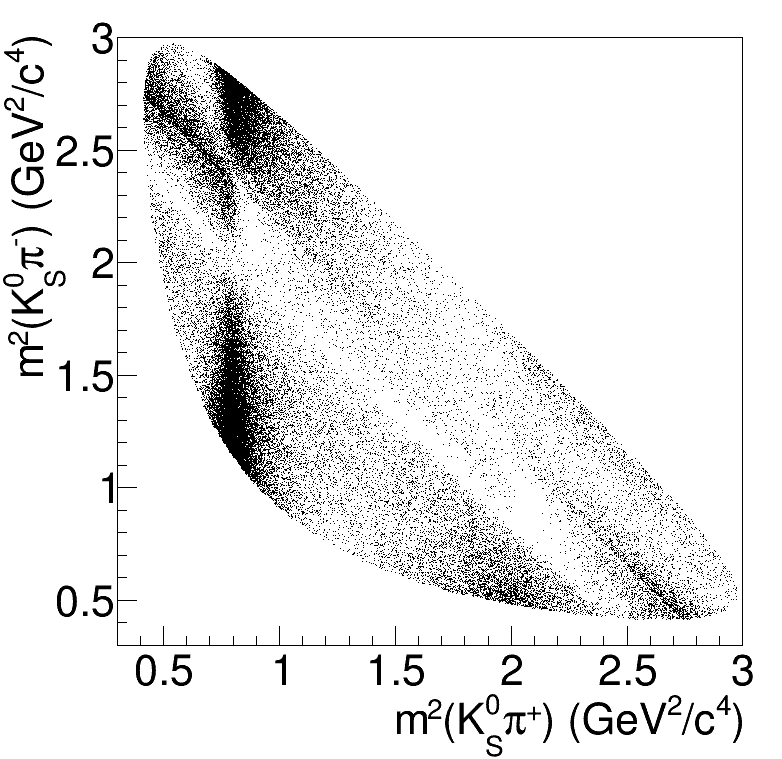
\includegraphics[width=0.45\textwidth]{dp_mc.png}
 \caption{Диаграмма Далица для распада \dbkpp.}
 \label{fig:kspp_dalitz}
\end{figure}

В случае распада \dkpp, параметры \rd и \deld (уравнение~\eqref{eq:rd_deltad}) являются функциями переменных Далица:
\begin{equation}
\begin{split}
 &\rd\dvar e^{i\deld\dvar} = \frac{\adbar\dvar}{\ad\dvar},\\
 & e^{i\deld\dvar} \equiv C\dvar + iS\dvar.
\end{split}
\end{equation}
Плотность распределения Далица для $D$-мезонов из распадов \bdk можно записать в виде
\begin{equation}\label{eq:dalitz_pdf_bdk}
\begin{split}
 \mcp_{B^+} &= \mcpdbar + \rb^2\mcpd    + 2\sqrt{\mcpd\mcpdbar}\left(x_+C + y_+S\right),\\
 \mcp_{B^-} &= \mcpd    + \rb^2\mcpdbar + 2\sqrt{\mcpd\mcpdbar}\left(x_-C - y_-S\right),
\end{split}
\end{equation}
где $\mcpd\equiv|\ad|^2$, $\mcpdbar\equiv|\adbar|^2$ и
\begin{equation}\label{eq:xy}
 x_{\pm} + iy_{\pm} \equiv \rb e^{i\left(\delb\pm\gphi\right)}.
\end{equation}
Зная функции \mcpd, $C$ и~$S$, можно измерить параметр~\gphi.  Обсуждение способов получения информации о функциях~$C$ и~$S$ приведено в пункте~\ref{sec:dalitz}.  

Чувствительность к параметрам~$x_{\pm}$ и~$y_{\pm}$ зависит от устройства функций $C$, $S$, \mcpd и~\mcpdbar (смотрите уравнение~\eqref{eq:dalitz_pdf_bdk}).  Для определения величины параметра~\gphi необходимо измерить все четыре параметра $x_{\pm}$ и $y_{\pm}$.  Необходимым условием для получения чувствительности ко всем этим параметрам является изменение разности фаз \deld (как функции переменных Далица) в широком диапазоне.  Наблюдения показывают, что распад \dnkpp обеспечивает достаточную чувствительность, а значительная вариация разности фаз~\deld достигается благодаря интерференции резонансных переходов $\dn\to\ks\rho$, $\dn\to\ks f_0$ и $\dn\to K^{*-}\pi^+$ (смотрите рисунок~\ref{fig:kspp_dalitz}).  

\paragraph{\boldmath Измерение угла \pphi с использованием осцилляций нейтральных $B$-мезонов.} Второй пример касается эффекта осцилляций нейтральных $B$-мезонов, рассмотренного в пункте~\ref{sec:mixing}.  Пусть в некоторое состояние $f_B$ могут распадаться нейтральные $B$-мезоны обоих ароматов.  Обозначим соответствующие амплитуды:
\begin{equation}
 \af \equiv \mca(\bn\to f_B),\quad \afbar \equiv \mca(\bnbar\to f_B).
\end{equation}
Если в начальный момент родился $B^0$-мезон, то амплитуда его перехода в состояние $f_B$ зависит от времени (в собственной системе отсчета) в соответствии с уравнением~\eqref{eq:flavor_states_evolution}:
\begin{equation}
 \ab(t) = e^{-imt-\Gamma t/2}\left[\af\cos\dmthalf + i\frac{q}{p}\afbar\sin\dmthalf\right].
\end{equation}
Соответствующая времязависимая плотность вероятности:
\begin{equation}\label{eq:time-dep-pb}
 \mcp_B(t) \propto e^{-\Gamma t}\left[1 + C_f\cos{\dmt} - S_f\sin{\dmt}\right],
\end{equation}
где 
\begin{equation}\label{eq:lamf}
 C_f = \frac{1-\lamfmsq}{1+\lamfmsq},\quad
 S_f = \frac{2\,\imag\,\lamf}{1+\lamfmsq},\quad
 \lamf=\frac{q}{p}\frac{\afbar}{\af}.
\end{equation}
\cpconj-асимметрия, определенная в~\eqref{eq:acp}, в рассматриваемом случае выражается через плотность вероятности~\eqref{eq:time-dep-pb} и является функцией времени~\cite{CarterSanda,BigiSanda}:
\begin{equation}\label{eq:time-dependent-acp}
 \acp\left(t\right) \equiv \frac{\mcpbar_B(t) - \mcp_B(t)}{\mcpbar_B(t) + \mcp_B(t)} = 
 S_f\sin{\dmt} - C_f\cos{\dmt}.
\end{equation}

При рассмотрении \cpconj-собственных конечных состояний $B$-мезонов и \cpconj-четностью $\eta_f$, амплитуда перехода в которые инвариантна относительно \cpconj-преобразования (например, $J/\psi\ks$), 
\begin{equation}\label{eq:qpbeta}
 \lamf = \eta_f e^{-2i\pphi},
\end{equation}
где угол \pphi определен в~\eqref{eq:ut_angles}, и асимметрия~\eqref{eq:time-dependent-acp} принимает вид
\begin{equation}\label{eq:time-dependent-acp-jpsi}
 \mca^{(J/\psi\ks)}_\cpconj\left(t\right) = -\sindbeta\sin{\dmt}.
\end{equation}

Описанный подход позволяет с высокой точностью измерить значение \sindbeta в распадах \bjpsiks.  Теоретическая неопределенность метода остается далеко за пределами чувствительности современных экспериментов.  В соответствии с общим принципом, чувствительность к \cpconj-нарушающему параметру обеспечена интерференцией двух процессов: $\bn\to f$ и $\bn\to\bnbar\to f$ (рисунок~\ref{fig:mixint}).

\begin{figure}[htb]
  \centering
  \includegraphics[width=0.4\textwidth]{mixing_interference}
  \caption{Схема интерференции процессов $\bn\to f$ и $\bn\to\bnbar\to f$.}
  \label{fig:mixint}
\end{figure}

Одной из проблем измерения параметра $2\pphi$ во времязависимом анализе \cpconj-собственных распадов $B$-мезонов является дискретная неопределенность $2\pphi\to\pi-2\pphi$.  Существует несколько способов разрешить эту неопределенность~\cite{Charles1998375,PhysRevD.56.7259,PhysRevD.61.116012}.  Наиболее привлекательный с экспериментальной точки зрения подход был рассмотрен в работе~\cite{bondar_gershon_krokovny}.  В этой работе предложено использовать распады \bdh, \dbkpp, где $h^0$ обозначает легкий нейтральный мезон (\pin, $\eta^{(\prime)}$ и $\omega$), и зависящую от времени в этом случае плотность распределения Далица для $D$-мезона из распадов \bdh:
\begin{equation}\label{eq:beta-dalitz-model-dep}
 \mcp_{q_B}\left(t\right) \propto e^{-\frac{t}{\btau}} \left[1 + q_B \left( \mca\dvar\cos{\dmt} + \mcs\dvar\sin{\dmt} \right)\right],
\end{equation}
где $q_B = 1$ ($q_B = -1$) соответствует \bn (\bnbar) при $t=0$ и
\begin{equation}
  \mca = \frac{\mcpd - \mcpdbar}{\mcpd + \mcpdbar},\quad
  \mcs = \frac{-2\eta_{h^0}(-1)^l\sqrt{\mcpd\mcpdbar}\sin{\left(\deld-2\pphi\right)}}{\mcpd + \mcpdbar},
\end{equation}
где $\eta_{h^0}$ --- \cpconj-четность $h^0$-мезона и $l$ --- орбитальный момент системы $Dh^0$.\footnote{Для распадов \bdstarh, \dbstdbpi, \dbkpp в функции \mcs возникает дополнительный множитель $-1$~\cite{bondar_gershon}.}  Значительное изменение разности фаз \deld в фазовом пространстве распада \dnkpp обеспечивает чувствительность к параметру $2\pphi$, значение которого может быть определено при известных функциях \mcpd, \mcpdbar и \deld.

% разработка алгоритма проверки и создание программ для измерения коэффициента усиления и линейности электронных модулей модернизированного калориметра Belle
% Bondar Gershon PRD 70, 091503(R)

\paragraph{\boldmath Классификация \cpconj-нарушающих распадов нейтральных $B$-мезонов.} \cpconj-нарушающие феномены в распадах нейтральных $B$-мезонов принято разделять на три группы:
\begin{enumerate}
 \item \emph{Прямое} нарушение \cpconj-симметрии. Реализуется при условии
 \begin{equation}
  \left|\frac{\afbar}{\af}\right|\neq 1.
 \end{equation}
 \item Нарушение \cpconj-симметрии \emph{в осцилляциях} нейтральных мезонов.  Реализуется при условии
 \begin{equation}
  \left|\frac{q}{p}\right|\neq 1.
 \end{equation}
 \item Нарушение \cpconj-симметрии \emph{в интерференции между осцилляциями и распадом}.  Реализуется при условии
 \begin{equation}
  \arg{\lamf}\neq 0.
 \end{equation}
\end{enumerate}
Приведенный пример нарушения \cpconj-симметрии в распадах \bjpsiks относится к \cpconj-нарушению в интерференции между осцилляциями и распадом.  %  В дальнейшем мы будем использовать эту терминологию.

%\clearpage
\section{Времязависимые измерения на асимметричной B-фабрике}\label{sec:dt_measurements}
Для изучения времязависимой \cpconj-асимметрии~\eqref{eq:time-dependent-acp} необходимо определять начальный аромат нейтрального $B$-мезона и измерять время между его рождением и распадом.  Эти требования приводят к большим экспериментальным сложностям, поскольку время жизни нейтральных $B$-мезонов примерно равно $1.5\ps$, а для определения аромата необходимо использовать информацию о частицах, рожденных вместе с $B$-мезоном.

Асимметричные ускорители встречных \ep-пучков высокой светимости, работающие вблизи резонанса~\ups ($B$-фабрики), были предложены для того, чтобы выполнение измерений такого рода было возможно.  Пара нейтральных $B$-мезонов, рожденных в процессе $\ep\to\ups\to\bn\bnbar$, находится в когерентном состоянии.  В соответствии с отрицательной \cconj-четностью \ups-резонанса, состояние пары $B$-мезонов антисимметрично относительно их перестановки.  Совместная плотность вероятности их распада во времена $t_1$ и $t_2$ (в собственных системах отсчета) может быть записана следующим образом~\cite{BaBarBook}:
\begin{equation}\label{eq:raw_coh_ampl}
 p(t_1,t_2) = p(\bn,t_1)p(\bnbar,t_2) - p(\bn,t_2)p(\bnbar,t_1),
\end{equation}
где $p(\bn, t_i)$ ($p(\bnbar, t_i)$) обозначает плотность вероятности того, что $B$ мезон, распавшийся в момент времени $t_i$, находится в состоянии с ароматом \bn (\bnbar). Плотности вероятности $p(\bn,t_i)$ и $p(\bnbar,t_i)$ определяются соотношением~\eqref{eq:flavor_states_evolution}.  

Пусть один из $B$-мезонов (\emph{помечающий}) распадается в состояние с определенным ароматом.  Тогда, благодаря антисимметричности состояния, в момент распада помечающего $B$-мезона, аромат второго (\emph{сигнального}) $B$-мезона определен и противоположен.

Рассмотрим плотность вероятности~\eqref{eq:raw_coh_ampl}, как функцию переменных $\dt\equiv (t_1 - t_2)$ и $(t_1+t_2)$. Проинтегрировав по переменной $(t_1+t_2)$, получим плотность вероятности распада сигнального $B$-мезона, как функцию переменной \dt
\begin{equation}\label{eq:time-dep-pb-tag}
 \mcp_B(\dt) \propto \bexp\left[1 + q_B\left(C_f\cos{\dmdt}-S_f\sin{\dmdt}\right)\right],
\end{equation}
где $q_B=1$ ($q_B=-1$) соответствует распаду сигнального $B$-мезона, как~\bn~(\bnbar).

Сумма масс двух $B$-мезонов близка к массе резонанса \ups, поэтому в системе \ups $B$-мезоны имеют небольшой импульс (примерно $300\mevc$) и характерный отлет около $30\mum$, измерить который с достаточной точностью не удается.  Для решения этой проблемы, энергии электронного и позитронного пучков делают разными, так что в лабораторной системе отсчета $B$-мезоны имеют достаточный для измерения отлета импульс и летят в направлении электронного пучка (в положительном направлении оси $z$, смотрите рисунок~\ref{fig:asym_collider}).  Используя малость импульса $B$-мезонов в системе отсчета \ups, можно получить кинематическое приближение
\begin{equation}\label{eq:kine-appr}
 \dt \approx \frac{\dz}{\cbgups},
\end{equation}
где \dz обозначает расстояние между вершинами распада $B$-мезонов в лабораторной системе отсчета, $\beta$ и $\gamma$ --- Лоренц-факторы резонанса \ups.  Таким образом, для получения разности времен распадов $B$-мезонов достаточно измерить координаты $z$ вершин их распадов.  Для $\bgups=0.425$ характерный отлет $B$-мезонов составляет примерно $200\mum$, поэтому для измерения координат вершин распадов необходим детектор с хорошей трековой системой, способной определять положение треков заряженных частиц с точностью лучше $100\mum$.

\begin{figure}[htb]
 \centering
  \includegraphics[width=0.7\textwidth]{collision_v2}
  \caption{Схема процесса $\ep\to\ups\to\bbbar$ на асимметричной $B$-фабрике.  \brec и \basc обозначают соответственно  сигнальный и помечающий $B$-мезоны.}
\label{fig:asym_collider}
\end{figure}

Анализ продуктов распада помечающего $B$-мезона позволяет получать информацию о его аромате (например, используя знак заряда лептона с большим импульсом или знак заряда $K$-мезона), необходимую для измерения \cpconj-асимметрии.  Таким образом, асимметричная $B$-фабрика позволяет выполнять измерения времязависимых \cpconj-асимметрий~\eqref{eq:time-dependent-acp}.

\section{Экспериментальный статус изучения CP-нарушения в распадах B-мезонов}\label{sec:angles}
В этом разделе представлен обзор основных экспериментальных результатов по изучению нарушения \cpconj-симметрии в распадах $B$-мезонов.

\subsection{CP-нарушение в древесных переходах}\label{sec:cpv_tree}
\paragraph{\boldmath Измерение \sindbeta в переходах \btoccs. } Кварковый процесс \btoccs происходит за счет древесного $b\to c$ перехода (рисунок~\ref{fig:btoccq_tree}) и петлевых $b\to s$ переходов (рисунок~\ref{fig:btoccq_loop}).  Амплитуду этого процесса можно представить в виде~\cite{bfacphys}
\begin{equation}\label{eq:amp_bccs}
 \mca_{\btoccs} = \vcb\vcsst\left(T + P^c - P^t\right) + \vub\vusst\left(P^u - P^t\right),
\end{equation}
где $T$ обозначает амплитуду древесного перехода, а $P^q$ --- амплитуду петлевого перехода с промежуточным кварком $q\in\{u, c, t\}$ (без соответствующих \ckm-множителей).  Вклад второго слагаемого со слабой фазой $V_{ub}$ в соотношении~\eqref{eq:amp_bccs} не приводит к значительным эффектам прямого \cpconj-нарушения, поскольку $|\vub\vusst/\vcb\vcsst|\sim\mco(\lambda^2)\sim 0.02$.  Доминирующая часть амплитуды~\eqref{eq:amp_bccs} пропорциональна $\vcb\vcsst$ и не содержит \cpconj-нарушающей фазы. 

\begin{figure}[htb]
\begin{minipage}[b]{0.5\textwidth}
 \centering
 \includegraphics[width=0.8\textwidth]{bccq_tree}
 \subcaption{}
 \label{fig:btoccq_tree}
\end{minipage}
\begin{minipage}[b]{0.5\textwidth}
 \centering
 \includegraphics[width=0.8\textwidth]{bccq_loop}
 \subcaption{}
 \label{fig:btoccq_loop}
\end{minipage}
 \caption{а) Древесный и б) петлевой вклады в переход \btoccq.}
 \label{fig:btoccq}
\end{figure}

Процесс \btoccs отвечает за распад $B^0$-мезона в \cpconj-собственное конечное состояние $\jpsi\ks$ с \cpconj-четностью $\eta_{\cpconj} = -1$ (мы пренебрегаем \cpconj-нарушением в системе нейтральных $K$-мезонов).  Благодаря тому, что \cpconj-нарушающая часть амплитуды распада \bjpsiks подавлена, этот распад позволяет изучать \cpconj-нарушение в интерференции между осцилляциями и распадом, как уже отмечалось.  При этом,
\begin{equation}\label{eq:acp_bccs}
 C_f(\bjpsiks) = 0,\quad S_f(\bjpsiks) = -\eta_\cpconj\sindbeta.
\end{equation}
Изучение времязависимой \cpconj-асимметрии в распадах \bjpsiks позволяет выполнять прецизионные измерения параметра \sindbeta (рисунок~\ref{fig:sindbeta_bccs}).  Самые точные на данный момент измерения выполнены в экспериментах \belle~\cite{belle_sinbeta}, \babar~\cite{babar_sinbeta} и \lhcb~\cite{lhcb_sinbeta}.  Комбинация всех существующих результатов измерений (включая использование конечных состояний $\jpsi K_L^0$, $\psiss\ks$, $\chi_{c1}\ks$ и некоторых других) дает~\cite{hfag} 
\begin{equation}\label{eq:sindbeta_bccs}
 \sindbeta^{(\btoccs)} = 0.691 \pm 0.017.
\end{equation}
Параметр \sindbeta является в настоящее время наиболее точно измеренным \cpconj-нарушающим параметром.

\begin{figure}[htb]
\begin{minipage}[b]{0.5\textwidth}
 \centering
 \includegraphics[width=\textwidth]{btoccsS_CP}
 \subcaption{}
 \label{fig:sindbeta_bccs}
\end{minipage}
\begin{minipage}[b]{0.5\textwidth}
 \centering
 \includegraphics[width=\textwidth]{phi1_rhoBar_etaBar}
 \subcaption{}
 \label{fig:beta_bccs}
\end{minipage}
 \caption{а) Результаты измерения \sindbeta в переходах \btoccs в различных экспериментах и б) ограничение на значение параметра \pphi, следующее из этих результатов~\cite{hfag}.}
 \label{fig:sinbeta}
\end{figure}

При известной величине \sindbeta, значение параметра \pphi может быть определено с точностью до двух дискретных неопределенностей
\begin{equation}
 \pphi \to \pi + \pphi,\quad \pphi \to \frac{\pi}{2} - \pphi.
\end{equation}
Первая из них не может быть разрешена любым измерением тригонометрических функций $2\pphi$, вторая же неопределенность может быть разрешена с помощью измерения параметра \cosdbeta.  При выборе области определения $\pphi\in[0\grad,180\grad)$, результат~\eqref{eq:sindbeta_bccs} соответствует решениям $(21.0\pm0.7)\grad$ и $(68.1\pm0.7)\grad$ (рисунок~\ref{fig:beta_bccs}).  

\paragraph{\boldmath Измерение \sindbeta в переходах \btocud. } Кварковый переход \btocud происходит благодаря единственной древесной амплитуде (рисунок~\ref{fig:btocudF}) и отвечает за распады нейтральных $B$-мезонов в такие конечные состояния, как $\dstarn h^0$ и $\dstarn\pi^+\pi^-$, где $h^0$ обозначает легкий мезон, состоящий из легких кварков: \pin, \etap и $\omega$.

\begin{figure}[htb]
\begin{minipage}[b]{0.5\textwidth}
 \centering
  \includegraphics[width=0.8\textwidth]{bcud}
 \subcaption{}
 \label{fig:btocudF}
\end{minipage}
\begin{minipage}[b]{0.5\textwidth}
 \centering
  \includegraphics[width=0.8\textwidth]{bucd}
 \subcaption{}
 \label{fig:btocudS}
\end{minipage}
 \caption{Кварковые переходы а) \btocud и б) \btoucd.}
 \label{fig:btocud}
\end{figure}

Рассматривая такие конечные состояния, как $D\pi^0$, где $D$-мезон распадается в \cpconj-собственное состояние, можно изучать времязависимую \cpconj-асимметрию и измерять \sindbeta аналогично случаю \btoccs переходов (смотрите уравнение~\eqref{eq:acp_bccs}).  Недавно группы \belle и \babar выполнили совместный анализ данных, используя набор из \cpconj-четных и \cpconj-нечетных конечных состояний, и получили следующее значение~\cite{markus_bdh}:
\begin{equation}\label{eq:sindbeta_bcud}
 \sindbeta^{(\btocud)} = 0.66 \pm 0.10\stat \pm 0.06\syst.
\end{equation}
Точность этого измерения значительно уступает точности измерения \sindbeta в переходах \btoccs~\eqref{eq:sindbeta_bccs}.  Тем не менее, этот результат важен с точки зрения ограничения возможных вкладов новой физики (НФ).  Кроме того, благодаря отсутствию петлевых вкладов, поправки к наблюдаемой величине нарушения \cpconj-симметрии в переходах \btocud меньше, чем соответствующие поправки в переходах \btoccs.  Основная поправка обусловлена кварковым переходом \btoucd (рисунок~\ref{fig:btocudS}), в результате которого происходят распады \bdnh.  Однако, амплитуда перехода \btoucd мала относительно амплитуды перехода \btocud, поскольку $|\vud\vcdst/\vcb\vudst|\approx 0.02$.  Кроме того, при достижении достаточной экспериментальной точности, вклад амплитуды \btoucd может быть учтен.

\paragraph{\boldmath Измерение \gphi в интерференции переходов \btocus и \btoucs.} В разделе~\ref{sec:cpv-phenom} обсуждалось прямое \cpconj-нарушение в распадах \bdk, возникающее благодаря интерференции процессов с переходами \btocus и \btoucs.  Изучение \cpconj-асимметрии в таких распадах позволяет получать информацию об угле \gphi~\ut.

Измерение \cpconj-асимметрии при реконструкции нейтральных $D$-мезонов в \cpconj-собственных конечных состояний (\glw-подход, уравнение~\eqref{eq:acp_glw}) выполнено с помощью анализа данных экспериментов CDF~\cite{cdf_glw}, \babar~\cite{babar_glw}, \belle и \lhcb~\cite{lhcb_glw_ads}.  Комбинация этих результатов дает значение
\begin{equation}
 \mca_{\cpconj+}^{(\glw)} =  0.125 \pm 0.017
\end{equation}
для конечных состояний с $\eta_\cpconj=1$ ($K^+K^-$, $\pi^+\pi^-$) и значение
\begin{equation}
 \mca_{\cpconj-}^{(\glw)} = -0.108 \pm 0.047
\end{equation}
для конечных состояний с $\eta_\cpconj=-1$ ($\ks\pin$, $\ks\omega$ и $\ks\varphi$).  На рисунке~\ref{fig:acp_glw} показаны результаты основных измерений $\mca_{\cpconj}^{(\glw)}$, включая результаты, полученные при анализе распадов $B^{\pm}\to D^{*}K^{\pm}$ и $B^{\pm}\to DK^{*\pm}$.

\begin{figure}[htb]
\begin{minipage}[b]{0.5\textwidth}
 \centering
  \includegraphics[width=0.99\textwidth]{A_cp}
 \subcaption{}
 \label{fig:acp_glw}
\end{minipage}
\begin{minipage}[b]{0.5\textwidth}
 \centering
  \includegraphics[width=0.99\textwidth]{A_ADS}
 \subcaption{}
 \label{fig:acp_ads}
\end{minipage}
 \caption{Результаты измерений а) $\mca_{\cpconj}^{(\glw)}$ (уравнение~\eqref{eq:acp_glw}) и б) $\mca_{\cpconj}^{(\ads)}$ (уравнение~\eqref{eq:acp_ads}) в распадах $B^{\pm} \to D^{(*)}_{\cpconj} K^{(*)\pm}$~\cite{hfag}.}
 \label{fig:acp_bdk}
\end{figure}

Измерение \cpconj-асимметрии при реконструкции нейтральных $D$-мезонов в состояниях с определенным ароматом (\ads-подход, уравнение~\eqref{eq:acp_ads}) выполнено в экспериментах CDF~\cite{cdf_ads}, \babar~\cite{babar_ads}, \belle~\cite{belle_ads} и \lhcb~\cite{lhcb_glw_ads}.  Наиболее точные результаты получены при реконструкции $D$-мезона в конечном состоянии $K^-\pi^+$.  Комбинация этих измерений дает
\begin{equation}
 \mca^{(\ads)}_{K\pi} = -0.41 \pm 0.06.
\end{equation}
На рисунке~\ref{fig:acp_ads} показаны результаты основных измерений $\mca^{(\ads)}$, включая результаты, полученные при реконструкции нейтральных $D$-мезонов в конечных состояниях $K^-\pi^+\pin$ и $K^-2\pi^+\pi^-$.

Использование распадов нейтральных $D$-мезонов в многочастичные \cpconj-самосопряженные состояния (например, \kspp, $\kspp\pin$ и $K^+K^-\pi^+\pi^-$) обеспечивает дополнительную чувствительность к параметру~\gphi~\cite{bondar,GGSZ}.  Конечное состояние \kspp позволяет проводить наиболее точные измерения, объединяя сильные стороны \glw- и \ads-подходов.  Основной вклад в распад \dnkpp вносят резонансы $\rho$, $f_0$ (приводя с \cpconj-собственном конечном состояниям $\ks\rho$ и $\ks f_0$) и $K^{*-}$ (приводя к конечному состоянию $K^{*-}\pi^+$ с определенным ароматом).  Интерференция этих резонансов увеличивает чувствительность к параметру \gphi и позволяет разрешить дискретные неопределенности, возникающие при извлечении величины этого параметра в \glw- и \ads-подходах.  

Как отмечалось ранее, для измерения \gphi в распадах \bdk, \dkpp необходимо иметь информацию об амплитуде распада $D$-мезона, включая разность фаз амплитуд распада \dn- и \dnbar-мезонов.  Распад \dnkpp представляет собой распад псевдоскалярной частицы в три псевдоскалярые частицы.  Это означает, что амплитуда распада является функцией в двумерном фазовом пространстве.  Информация об амплитуде может быть получена с помощью построения модели амплитуды трехчастичного распада, либо модельно-независимо.  В последнем случае фазовое пространство разделяется на области; для каждой области измеряется средние значения модуля амплитуды, синуса и косинуса комплексной фазы.  Подробнее эти вопросы обсуждаются в разделе~\ref{sec:dalitz}.

Результаты измерения \cpconj-нарушения в распадах \bdk, \dkpp принято выражать в декартовых параметрах $x_{\pm}$ и $y_{\pm}$ (уравнение~\eqref{eq:xy}).  Модельно-зависимые измерения этих параметров выполнены в экспериментах \babar~\cite{babar_gamma_dalitz_model}, \belle~\cite{belle_gamma_dalitz_model} и \lhcb~\cite{lhcb_gamma_dalitz_model} (рисунок~\ref{fig:bdk_unbinned_dalitz}).  Модельно-независимые измерения выполнены в экспериментах \belle~\cite{belle_gamma_binned_dalitz} и \lhcb~\cite{lhcb_gamma_binned_dalitz} (рисунок~\ref{fig:bdk_binned_dalitz}).

\begin{figure}[htb]
\begin{minipage}[b]{0.5\textwidth}
 \centering
  \includegraphics[width=0.99\textwidth]{D_DalitzKxvsy}
 \subcaption{}
 \label{fig:bdk_unbinned_dalitz}
\end{minipage}
\begin{minipage}[b]{0.5\textwidth}
 \centering
  \includegraphics[width=0.99\textwidth]{D_DalitzKmodIndxvsy}
 \subcaption{}
 \label{fig:bdk_binned_dalitz}
\end{minipage}
 \caption{Результаты измерений параметров $x_{\pm}$ и $y_{\pm}$, определенных в уравнении~\eqref{eq:xy}, в распадах \bdk, \dkpp с помощью а) модельно-зависимого и б) модельно-независимого анализа диаграмм Далица~\cite{hfag}.}
 \label{fig:bdk_dalitz}
\end{figure}

Группы \babar, \belle и \lhcb представили ограничения на величину параметра~\gphi, основываясь на комбинации всех полученных результатов:
\begin{equation}
 \begin{aligned}
  \gphi &= (69^{+17}_{-16})\grad     && (\babar~\text{\cite{babar_gamma}}), \\
  \gphi &= (68^{+15}_{-14})\grad     && (\belle~\text{\cite{belle_gamma}}), \\
  \gphi &= (70.9^{+7.1}_{-8.5})\grad && (\lhcb~\text{\cite{lhcb_gamma}}). \\
 \end{aligned}
\end{equation}
Комбинация этих результатов позволяет уменьшить неопределенность значения~\gphi приблизительно до~$6\grad$.

%\clearpage
% \subsection{CP-нарушение в петлевых переходах}\label{sec:cpv_loop}
% \begin{figure}[htb]
% \begin{minipage}[b]{0.32\textwidth}
%  \centering
%   \includegraphics[width=0.9\textwidth]{bsss}
%  \subcaption{}
%  \label{fig:bsss}
% \end{minipage}
% \begin{minipage}[b]{0.32\textwidth}
%  \centering
%   \includegraphics[width=0.9\textwidth]{bsll}
%  \subcaption{}
%  \label{fig:bsll}
% \end{minipage}
% \begin{minipage}[b]{0.32\textwidth}
%  \centering
%   \includegraphics[width=0.9\textwidth]{bsgamma}
%  \subcaption{}
%  \label{fig:bsgamma}
% \end{minipage}
%  \caption{Примеры петлевых переходов.}
%  \label{fig:loops}
% \end{figure}
% Распады, идущие в главном приближении посредством петлевых переходов, интересны с точки зрения проверки СМ, поскольку в петлях могут проявляться вклады НФ.  Примерами таких переходов являются радиационные и полулептонные переходы $b\to \{s,d\}\{\gamma,l^+l^-,\nu\overline{\nu}\}$, а также кварковые переходы \btosss, \btodds и \btossd (рисунок~\ref{fig:loops}).  
% 
% Интерпретация \cpconj-нарушающих феноменов в петлевых переходах осложняется тем, что необходимо учитывать вклады трех переходов с разными промежуточными кварками и разными слабыми фазами.  Эффекты адронизации также могут влиять на величину наблюдаемых \cpconj-нарушающих параметров.
% 
% \paragraph{\boldmath Поиск \cpconj-нарушения в адронных конечных состояниях. } Аналогично уравнению~\eqref{eq:amp_bccs}, амплитуду перехода \btosss можно представить в виде
% \begin{equation}\label{eq:amp_bsss}
%  \mca_{\btosss} = (P_c - P_u)\vcb\vcsst + (P_t - P_u)\vtb\vtsst.
% \end{equation}
% Относительная слабая фаза между двумя слагаемыми в уравнении~\eqref{eq:amp_bsss} мала и обозначается через
% \begin{equation}
%  \pphi_s\equiv\arg{\left(-\frac{\vts\vtbst}{\vcs\vcbst}\right)}.
% \end{equation}
% Поиск \cpconj-нарушения в распадах, обусловленных этим переходом ($B^+\to \varphi K^+$, $B^+\to\etap K^+$), является важным инструментом для проверки СМ.  Поиски \cpconj-нарушения в этих модах не выявили отклонений от СМ~\cite{babar_btokkk,lhcb_btokkk,belle_btoetapk,babar_btoetap}.  Комбинации измерений \cpconj-асимметрии (смотрите уравнение~\eqref{eq:acp}) согласуются с нулем: 
% \begin{equation}
%  \mca_\cpconj(B^+\to \varphi K^+) = 0.016\pm0.013,\quad \mca_\cpconj(B^+\to\etap K^+) = 0.004\pm0.011.
% \end{equation}
% 
% Относительная слабая фаза между петлевыми вкладами в переходе \btodds также равна $\pphi_s$, поэтому \cpconj-нарушающие эффекты в распадах $B^+\to \ks\pi^+$ ожидаются малыми, что согласуется с наблюдениями~\cite{belle_btohh,babar_btokk,lhcb_btokk}.
% 
% Б\emph{о}льшие \cpconj-нарушающие эффекты можно ожидать в переходах \btossd, поскольку относительная фаза петлевых амплитуд равна \pphi.  Распады, соответствующие этому кварковому переходу ($B^+\to \etap\pi^+$, $B^+\to\ks K^+$), однако, имеют небольшие вероятности, поэтому существующие наблюдения сильно ограничены статистически~\cite{lhcb_btokkk,belle_btoetapk,belle_btohh,babar_btokk,lhcb_btokk}.
% 
% \paragraph{\boldmath Измерение \sindbetaeff. } Переходы \btosss можно использовать для изучения времязависимой \cpconj-асимметрии (смотрите раздел~\ref{sec:cpv-phenom} и пункт~\ref{sec:cpv_tree}).  Параметр $S_f$ при этом выражают через \pphieff --- эффективный параметр \pphi:
% \begin{equation}
%  S_f^{(\btosss)} = -\eta_f\sindbetaeff.
% \end{equation}
% Величина \pphieff может отличаться от величины параметра \pphi, измеряемого в переходах \btoccs, из-за поправок, возникающих за счет петлевых вкладов.
% 
% \begin{figure}[htb]
% \begin{minipage}[b]{0.5\textwidth}
%  \centering
%   \includegraphics[width=0.99\textwidth]{sPengS_CP_woKsPi0Pi0}
%  \subcaption{}
%  \label{fig:bsssS}
% \end{minipage}
% \begin{minipage}[b]{0.5\textwidth}
%  \centering
%   \includegraphics[width=0.99\textwidth]{sPengC_CP_woKsPi0Pi0}
%  \subcaption{}
%  \label{fig:bsssC}
% \end{minipage}
%  \caption{Результаты измерения а) \sindbetaeff и б) коэффициента $C$ (смотрите уравнение~\eqref{eq:time-dependent-acp}) в кварковых переходах \btosss~\cite{hfag}.}
%  \label{fig:betaeff}
% \end{figure}
% 
% На рисунке~\ref{fig:bsssS} показаны результаты измерений параметра \sindbetaeff в распадах нейтральных $B$-мезонов, идущих  благодаря переходам \btosss.  На рисунке~\ref{fig:bsssC} приведены соответствующие результаты измерений коэффициента $C_f$, отвечающего за прямое нарушение \cpconj-симметрии.  Точность всех этих результатов ограничена статистической неопределенностью; наиболее точные измерения выполнены в распадах $\bn\to\etap K^0$~\cite{babar_betaeff,belle_betaeff} и $B^0\to$ $\varphi K^0$~\cite{babar_btopipi,belle_betaeff2}.  Проведенные измерения не выявили значимых отклонений от ожиданий СМ.  Комбинация измерений в переходах \btoqqs приводит к значению
% \begin{equation}
%  \sindbetaeff = 0.655 \pm 0.032,
% \end{equation}
% согласующемуся со значением \sindbeta, измеренному в переходах \btoccs.
% 
% \paragraph{\boldmath Поиск \cpconj-нарушения в переходах $b\to q\gamma$ и $b\to ql^+l^-$. } Переходы $b\to q\gamma$ и $b\to ql^+l^-$ позволяют выполнить множество измерений, дающих информацию о моделях физики за пределами СМ~\cite{tim}.  Неопределенности предсказаний СМ для этих переходов, связанные со взаимодействием адронов, обычно меньше, чем для переходов, рассмотренных выше, поскольку некоторые частицы конечного состояния не взаимодействуют сильным образом.
% 
% Комбинация измерений \cpconj-асимметрии в инклюзивных переходах $b\to s$ дает результат~\cite{hfag,babar_btoxsgamma,babar_btoxsll}
% \begin{equation}
%  \acp(B\to X_s\gamma) = 0.015 \pm 0.020,\quad \acp(B\to X_s l^+l^-) = 0.04\pm0.11.
% \end{equation}
% Эти величины получены посредством комбинирования результатов для различных эксклюзивных мод.  
% 
% Более точные измерения \acp выполнены при изучении эксклюзивных распадов~\cite{hfag,babar_bsgamma,lhcb_bsgamma,lhcb_btokstmumu}
% \begin{equation}
%  \begin{split}
%   \acp(B^0\to K^{*0}\gamma)     &= -0.002 \pm 0.015, \\
%   \acp(B^0\to K^{*0}\mu^+\mu^-) &= -0.035 \pm 0.024 \pm 0.003,\\
%   \acp(B^+\to K^{+}\mu^+\mu^-) &= \phantom{-}0.012 \pm 0.017 \pm 0.001.
%  \end{split}
% \end{equation}
% В работе~\cite{lhcb_btokstmumu} \cpconj-асимметрия измерена для различных значений квадрата инвариантной массы системы $\mu^+\mu^-$ в распадах $B^0\to K^{*0}\mu^+\mu^-$ и $B^+\to K^{+}\mu^+\mu^-$ (рисунок~\ref{fig:btosll}).  Полученные результаты не выявили значимого \cpconj-нарушения.  В работе~\cite{lhcb_btokstmumu_angular} проведен полный угловой анализ распада $B^0\to K^{*0}\mu^+\mu^-$.  Результат этого анализа показал отклонение от гипотезы соблюдения \cpconj-симметрии на уровне $3.4$ стандартных отклонений.
% 
% \begin{figure}[htb]
% \begin{minipage}[b]{0.5\textwidth}
%  \centering
%   \includegraphics[width=0.99\textwidth]{acp_btokpmumu}
%  \subcaption{}
%  \label{fig:acp_btokpmumu}
% \end{minipage}
% \begin{minipage}[b]{0.5\textwidth}
%  \centering
%   \includegraphics[width=0.99\textwidth]{acp_btokstmumu}
%  \subcaption{}
%  \label{fig:acp_btokstmumu}
% \end{minipage}
%  \caption{\acp для различных значений $q^2 \equiv m^2(\mu^+\mu^-)$, измеренная группой LHCb в распадах а) $B^+\to K^+\mu^+\mu^-$ и б) $B^0\to K^{*0}\mu^+\mu^-$~\cite{lhcb_btokstmumu}.}
%  \label{fig:btosll}
% \end{figure}
% 
% Согласно СМ, испущенный в переходе $b\to q\gamma$ фотон почти полностью поляризован.  Эта особенность уменьшает наблюдаемое \cpconj-нарушение в интерференции между осцилляциями и распадом, поскольку фотоны в переходах $\bnbar\to\overline{K}^{*0}\gamma\to\ks\pin\gamma$ и $\bn\to {K}^{*0}\gamma\to\ks\pin\gamma$ поляризованы преимущественно в левую и правую стороны, соответственно, а значит интерференция этих конечных состояний подавлена.  Величина $S_f$ (уравнение~\eqref{eq:time-dependent-acp}) в этом случае содержит дополнительный множитель $\sin{2\Phi}$, где $\tan{\Phi}$ равен отношению амплитуд с подавленной и разрешенной поляризациями~\cite{gamma_polar_theory1,gamma_polar_theory2}.  Анализ времязависимой \cpconj-асимметрии в распадах нейтральных $B$-мезонов через переход $b\to s\gamma$ позволяет измерить поляризацию фотона, поскольку
% \begin{equation}
%  S^{(b\to s\gamma)} = -\eta_\cpconj\sin{2\Phi}\sindbetaeff.
% \end{equation}
% Измерения, выполненные для распадов $\bn\to\ks\pin\gamma$~\cite{belle_photon_polar,babar_photon_polar} и $\bn\to\ks\rho^0\gamma$~\cite{belle_photon_polar2,babar_photon_polar2}, не выявили значимого \cpconj-нарушения, что согласуется с ожидаемой величиной поляризации фотона.

%\clearpage
\subsection{CP-нарушение в интерференции древесных и петлевых переходов}\label{sec:cpv_tree_and_loop}
Некоторые адронные распады $B$-мезонов имеют сопоставимые вклады от древесных и петлевых амплитуд.  К ним относятся распады, обусловленные кварковыми переходами \btouud, \btouus, и, во многих случаях, \btodds и \btoddd (рисунок~\ref{fig:buud}).  Интерференция между древесными и петлевыми вкладами может приводить к прямому \cpconj-нарушению.  Интерпретация величины наблюдаемого \cpconj-нарушения в терминах фундаментальных параметров в этих случаях проблематична из-за неопределенностей, связанных со взаимодействием адронов.  Для уменьшения этих неопределенностей часто привлекают соображения, основанные на приблизительной симметрии легких кварков.

\begin{figure}[htb]
\begin{minipage}[b]{0.5\textwidth}
 \centering
  \includegraphics[width=0.8\textwidth]{buud_tree}
 \subcaption{}
 \label{fig:buud_tree}
\end{minipage}
\begin{minipage}[b]{0.5\textwidth}
 \centering
  \includegraphics[width=0.8\textwidth]{buud_loop}
 \subcaption{}
 \label{fig:buud_loop}
\end{minipage}
 \caption{а) Древесный и б) петлевой вклады в переход \btouud.}
 \label{fig:buud}
\end{figure}

\paragraph{\boldmath Прямое \cpconj-нарушение в переходах \btouuq. } Прямое \cpconj-нарушение в распадах $B^0\to K^+\pi^+$ надежно установлено несколькими группами~\cite{lhcb_btokpi_cpv,babar_btopipi,belle_btohh,cdf_btohh_cpv}.  Комбинация всех измерений приводит к величине~\cite{hfag}
\begin{equation}
 \acp\left(\bn\to K^+\pi^-\right) = -0.082\pm0.006.
\end{equation}
Гораздо более неожиданный результат был получен для разности
\begin{equation}
 \Delta\acp\left(B\to K\pi\right) = \acp\left(\bn \to K^+\pi^-\right) - \acp\left(B^+ \to K^+\pin\right).
\end{equation}
Измеренное значение $\acp\left(B^+ \to K^+\pi^0\right) = 0.040\pm0.021$~\cite{belle_btohh,babar_btohh} приводит к
\begin{equation}
 \Delta\acp\left(B\to K\pi\right) = -0.122 \pm 0.022.
\end{equation}
Причина отличия этой величины от нуля не ясна, поскольку распады $\bn \to K^+\pi^-$ и $B^+ \to K^+\pin$ отличаются только спектаторным кварком первого поколения.  Интересным развитием этих результатов было бы измерение \cpconj-асимметрии в распадах $B\to K^*\pi$ и $B\to K\rho$ с векторными мезонами в конечном состоянии.  

% \begin{figure}[htb]
% \begin{minipage}[b]{0.5\textwidth}
%  \centering
%   \includegraphics[width=0.8\textwidth]{lhcb_cpv_ppp}
%  \subcaption{}
%  \label{fig:lhcb_cpv_ppp}
% \end{minipage}
% \begin{minipage}[b]{0.5\textwidth}
%  \centering
%   \includegraphics[width=0.8\textwidth]{lhcb_cpv_ppk}
%  \subcaption{}
%  \label{fig:lhcb_cpv_ppk}
% \end{minipage}
% \\
% \begin{minipage}[b]{0.5\textwidth}
%  \centering
%   \includegraphics[width=0.8\textwidth]{lhcb_cpv_kkk}
%  \subcaption{}
%  \label{fig:lhcb_cpv_kkk}
% \end{minipage}
% \begin{minipage}[b]{0.5\textwidth}
%  \centering
%   \includegraphics[width=0.8\textwidth]{lhcb_cpv_kkp}
%  \subcaption{}
%  \label{fig:lhcb_cpv_kkp}
% \end{minipage}
%  \caption{Распределения по количеству распадов $B^+$- и $B^-$-мезонов для различных значений двухчастичных инвариантных масс для конечных состояний а) $\pi^+\pi^-\pi^{\pm}$, б) $\pi^+\pi^-K^{\pm}$, в) $K^+K^-K^{\pm}$ и г) $K^+K^-\pi^{\pm}$~\cite{lhcb_btohhh_cpv}.} 
%  \label{fig:lhcb_cpv_btohhh}
% \end{figure}

%Группа \lhcb выполнила поиск \cpconj-нарушения в трехчастичных распадах $B^{\pm}\to\pi^+\pi^-\pi^{\pm},\,\pi^+\pi^-K^{\pm},\,K^+K^-K^{\pm}$ и $K^+K^-\pi^{\pm}$ с помощью модельно-независимой процедуры, сравнивая распределения событий в различных кинематических областях (рисунок~\ref{fig:lhcb_cpv_btohhh}), и обнаружила значимые \cpconj-нарушающие эффекты в некоторых кинематических областях~\cite{lhcb_btohhh_cpv}.

\paragraph{\boldmath Определение величины \aphi. } Времязависимая \cpconj-асимметрия (смотрите уравнение~\eqref{eq:time-dependent-acp}) в распадах $\bn\to\pi^+\pi^-$ была изучена в экспериментах \belle~\cite{belle_btopipi}, \babar~\cite{babar_btopipi} и \lhcb~\cite{lhcb_btopipi}.  Комбинация результатов этих измерений дает~\cite{hfag}
\begin{equation}\label{eq:CSpipi}
 S_{\pi^+\pi^-} = -0.66 \pm 0.06,\quad
 C_{\pi^+\pi^-} = -0.31 \pm 0.05,
\end{equation}
и свидетельствует о наблюдении и прямого \cpconj-нарушения и \cpconj-нарушения в интерференции между осцилляциями и распадом.  Прямое \cpconj-нарушение указывает на значительный вклад петлевых переходов в распад $\bn\to\pi^+\pi^-$ и осложняет интерпретацию величины $S_{\pi^+\pi^-}$ в терминах параметров \ckm-матрицы.  

В работе~\cite{alpha_isospin} показано, что информацию о параметре \aphi можно извлечь, используя изоспиновую симметрию в распадах $B^+\to\pi^+\pi^0$, $\bn\to\pi^+\pi^-$ и $\bn\to\pi^0\pi^0$.  Можно получить соотношение
\begin{equation}
 S_{\pi^+\pi^-} = \sqrt{1-C_{\pi^+\pi^-}^2}\sin\left(2\aphi - 2\Delta\alpha\right),
\end{equation}
где параметр $2\Delta\alpha$ должен быть определен из изоспинового анализа.  Значение параметра \aphi в этом подходе может быть определено с точностью до восьмизначной дискретной неопределенности.  Точность определения параметра \aphi в распадах $B\to\pi\pi$ ограничена точностью измерения вероятности распада $\bn\to\pin\pin$ и соответствующей \cpconj-асимметрии~\cite{hfag,babar_btopipi,belle_pit_alpha}
\begin{equation}
 \br\left(\bn\to\pin\pin\right) = (1.17\pm0.13)\times 10^{-6},\quad \acp\left(\bn\to\pin\pin\right) = 0.43\pm0.27.
\end{equation}

Подобный анализ может быть выполнен для распадов $B\to\rho\rho$.  Анализ этих состояний усложняется ввиду различных возможных поляризаций двух векторных мезонов, а также из-за достаточно большой ширины $\rho$-мезона.  Установлено, однако, что в этих распадах доминирует продольная поляризация~\cite{babar_btorhoprho,belle_btorhoprho}.  Другим преимуществом использования пары $\rho$-мезонов является удобство экспериментального изучения состояния $\rho^0\rho^0$, поскольку в конечном состоянии регистрируются только четыре заряженные частицы.  Комбинация измерений времязависимой \cpconj-асимметрии в распадах $\bn\to\rho^+\rho^-$ приводит к значениям~\cite{hfag,babar_btorhoprho,belle_btorhoprho}
\begin{equation}
 S_{\rho^+\rho^-} = -0.14 \pm 0.13,\quad
 C_{\rho^+\rho^-} = -0.00 \pm 0.09.
\end{equation}
Малость параметра $C_{\rho^+\rho^-}$ указывает на менее значимый вклад петлевых переходов, чем в распаде $\bn\to\pi^+\pi^-$.  Этот вывод подтверждается и анализом изоспиновых соотношений.

Альтернативный способ выделения петлевых вкладов предложен в работах~\cite{btorhopi_theory1,btorhopi_theory2}.  Выполняя анализ динамики трехчастичного распада $\bn\to\pi^+\pi^-\pin$ можно выделить вклад петлевых переходов и определить значение параметра \aphi без неопределенностей. Ограничения на величину параметра \aphi, полученные с помощью этого подхода, в настоящий момент уступают измерениям в распадах $B\to\pi\pi$ и $B\to\rho\rho$~\cite{belle_rhopi,belle_rhopi_prd,babar_rhopi}.  На рисунке~\ref{fig:alpha} показаны ограничения на значение параметра \aphi, полученные из анализе распадов $B\to\pi\pi$, $B\to\rho\pi$ и $B\to\rho\rho$.  Комбинация этих ограничений приводит к значению~\cite{ckmfitter}
\begin{equation}
 \aphi = (87.6^{+3.5}_{-3.3})\grad.
\end{equation}

\begin{figure}[H]
 \centering
  \includegraphics[width=0.51\textwidth]{B2UUAll_alpha}
 \caption{Ограничения на значение параметра \aphi из анализа распадов $B\to\pi\pi$, $B\to\rho\pi$ и $B\to\rho\rho$~\cite{ckmfitter}.}
 \label{fig:alpha}
\end{figure}

%\clearpage
\subsection{Комбинация измерений параметров \ckm-матрицы}
Изучение \cpconj-нарушения в распадах $B$-мезонов позволяет измерить каждый из трех углов \ut.  Длины сторон \ut также могут быть измерены~\cite{pdg}.  Получившаяся переопределенная система ограничений, объединяющая различные экспериментальные результаты, позволяет выполнять прецизионную проверку соотношений треугольника для \ut, а значит и проверку \km-механизма.  Любое противоречие может свидетельствовать о проявлении эффектов НФ.

%Количественная оценка согласия наблюдений со СМ может быть получена, например, с помощью изъятия прямых измерений некоторого параметра и определения значения этого параметра, используя остальные ограничения.  Результаты прямых измерений должны быть в согласии с полученным значением в случае справедливости СМ; значимое расхождение можно интерпретировать как проявление эффектов НФ.

Две группы занимаются систематическим анализом всех доступных экспериментальных данных и их интерпретаций с учетом теоретических результатов~\cite{ckmfitter,utfit}.  На рисунке~\ref{fig:ckmfitter} показаны усредненные экспериментальные ограничения на параметры \ut, полученные одной из этих групп.  Анализ показывает, что, при текущей точности измерения параметров \ut, составляющей в среднем $5\%$-$10\%$, значимых нарушений СМ не выявлено.

\begin{figure}[htb]
 \centering
  \includegraphics[width=0.9\textwidth]{rhoeta_large}
 \caption{Комбинация измерений параметров \ckm-матрицы~\cite{ckmfitter}.}
 \label{fig:ckmfitter}
\end{figure}

Таким образом, необходимо дальнейшее повышение точности измерений.  Оценки потенциальных возможностей реализуемых в настоящее время экспериментов (\lhcb и \belleii) показывают, что в ближайшие $5$-$10$ лет возможно достижение точности $1\%$-$3\%$ в измерении основных параметров~\ut~\cite{Gershon:2016fda}.


             % Глава 1
\chapter{Модельно-независимое получение параметров с использованием многочастичных распадов} \label{chapt2}
В этой главе описан модельно-независимый подход к анализу многочастичных распадов (раздел~\ref{sec:dalitz}) и предложены программы исследований для симметричной Чарм-Тау-фабрики (раздел~\ref{sec:charm-tau-phenom}) и асимметричной $B$-фабрики,  а также для эксперимента \lhcb (раздел~\ref{sec:b-factory-phenom}), основанные на этом подходе.  

В пункте~\ref{sec:charm_mixing_measurement_at_ctau} описан впервые предложенный в работе автора диссертации~\cite{mixing} метод модельно-независимого измерения параметров смешивания $D$-мезонов в когерентных распадах \ddbar-пар.  В пункте~\ref{sec:time-dependent-charm-mixing} описан впервые предложенный в той же работе метод модельно-независимого измерения параметров смешивания $D$-мезонов во времязависимом анализе распадов \dkpp, который в последствии был использован для анализа данных группой \lhcb~\cite{lhcb_dkspp_mixing}.  

В пункте~\ref{sec:gamma-and-charm-mixing} рассмотрено влияние осцилляций $D$-мезонов на наблюдаемое значение параметра \gphi при модельно-независимом измерении в распадах \bdk, \dkpp и описана модификация процедуры измерения \gphi, при которой осцилляции $D$-мезонов смещают наблюдаемое значение не больше чем на $0.2\grad$, впервые предложенная в работе автора~\cite{mixing}.  
В пункте~\ref{sec:gamma-and-dcpv-in-charm} рассмотрено влияние нарушение \cpconj-симметрии в распадах \dnkpp на наблюдаемое значение параметра~\gphi при модельно-независимом измерении в распадах \bdk, \dkpp и описана модификация процедуры измерения, не предполагающая сохранение \cpconj-симметрии в распадах~\dnkpp, впервые преложенная в работе автора~\cite{bdpv_cpv}.  

В пункте~\ref{sec:model-independent-beta} описан метод модельно-независимого измерения параметра \pphi во времязависимом анализе распадов \bdsth, \dbkpp, впервые предложенный в работе автора~\cite{belle_beta_binned_dalitz}.  Первая реализация этого метода, выполненная с данными эксперимента \belle, описана в главе~\ref{sec:bdsth}.

\section{Модельно-независимый анализ трехчастичных распадов} \label{sec:dalitz}
Рассмотрение многочастичных распадов зачастую позволяет преодолеть ограничения феноменологических подходов, основанных на анализе двухчастичных распадов $B$- и $D$-мезонов.  Так, анализ трехчастичного распада $\bn\to\pi^+\pi^-\pin$ позволяет разрешить четырехкратную дискретную неопределенность при измерении параметра \aphi (пункт~\ref{sec:cpv_tree_and_loop});  $D$-мезоны из распадов \bdk, реконструированные в конечном состоянии \kspp, позволяют получить параметр \gphi (раздел~\ref{sec:cpv-phenom});  времязависимый анализ распадов \bdh, \dbkpp позволяет измерить \cosdbeta и разрешить двузначную дискретную неопределенность при измерении параметра~$2\pphi$ (раздел~\ref{sec:cpv-phenom}).  

С другой стороны, использование многочастичных распадов приводит к сложностям, связанным с ограниченным знанием динамики распада.  Амплитуда многочастичного распада является (комплексной) функцией, определенной в фазовом пространстве конечного состояния.  В отличие от модуля, комплексная фаза амплитуды многочастичного распада не может быть измерена непосредственно.  Чаще всего информацию о комплексной фазе амплитуды многочастичного распада получают исходя из модельных предположений.  
Такой подход нельзя считать удовлетворительным, поскольку он приводит к неустранимой и сложно оцениваемой неопределенности, связанной как со значением параметров модели, так и с обоснованностью применения той или иной модели.  В экспериментах с большой статистикой эти неопределенности могут стать доминирующим фактором, определяющим точность измерений.

В работе~\cite{GGSZ} была предложена идея модельно-независимого анализа распадов \dnkpp для измерения параметра \gphi в распадах \bdk.  Для измерения параметра \gphi нет необходимости знать величину \deld (уравнение~\eqref{eq:rd_deltad}) в каждой точке фазового пространства.  Достаточным является знание среднего значения $\sin\deld$ и $\cos\deld$ для нескольких областей фазового пространства.  А именно, введем параметры
\begin{equation}\label{eq:ki}
 \ki = \frac{\int\ddlzarea\left|\ad\right|^2 \ddlz}
            {\int\limits_{\mcd}\left|\ad\right|^2 \ddlz},\quad
 \kbi = \frac{\int\ddlzarea\left|\adbar\right|^2 \ddlz}
            {\int\limits_{\mcd}\left|\adbar\right|^2 \ddlz},
\end{equation}
и
\begin{equation}\label{eq:csi}
  \zi \equiv \ci + i\si = 
            \frac{\int\ddlzarea
            \left|\ad\right|\left|\adbar\right|
            e^{i\deld}\,\ddlz}
            {\int\ddlzarea\left|\ad\right|^2 \ddlz 
             \int\ddlzarea\left|\adbar\right|^2 \ddlz}
            ,
\end{equation}
где индекс $i$ обозначает номер области фазового пространства, $\mcd$ --- полное фазовое пространство и $\mcd_i$ --- область фазового пространства, соответствующую номеру~$i$.  Для параметров \ki и \kbi выполняются нормировочные условия
\begin{equation}
 \sum\limits_i \ki = 1,\quad \sum\limits_i \kbi = 1.
\end{equation}

Предполагая отсутствие \cpconj-нарушения в распадах $D$-мезонов, т.е. используя соотношение $\ad\dvar\equiv\adbar\dvarinv$, можно оптимизировать способ разбиения диаграммы Далица распада \dnkpp: выбрать $2\mcn$ области симметрично относительно перестановки $\mpsq\leftrightarrow\mmsq$.  Номера областей $i$ при этом принимают значения от $-\mcn$ до $\mcn$, исключая $0$, такие, что инверсия знаков номеров областей $i\to -i$ соответствует перестановке $\mpsq\leftrightarrow\mmsq$. При таких договоренностях выполняются соотношения
\begin{equation}\label{eq:cp-conserv-relations}
 \zi \equiv Z^*_{-i}\quad (C_i\equiv C_{-i},\quad S_i\equiv -S_{-i}),\quad \kbi \equiv \kmi.
\end{equation}

В работах~\cite{Bondar2006,Bondar2008} были изучены вопросы о том, как выбрать значение \mcn и из каких соображений выбирать форму областей.  Поясним основные выводы, полученные в этих работах, на примере измерения параметра \gphi в распадах \bdk.  Проинтегрируем уравнение~\eqref{eq:dalitz_pdf_bdk} по области $i$ и выразим результат через введенные параметры:
\begin{equation}\label{eq:dalitz_pdf_bdk_binned}
 N_i^{\pm} \propto \kmpi + \rb^2\kpmi + 2\sqrt{\ki\kmi}\left(x_{\pm}C_i+y_{\pm}S_i\right).
\end{equation}
Если неизвестные параметры \ki, \ci и \si получить из независимых измерений (способ измерения этих параметров обсуждается в пункте~\ref{sec:cs_measurement}), то из соотношений~\eqref{eq:dalitz_pdf_bdk_binned} можно получить интересующие параметры~$x_{\pm}$ и~$y_{\pm}$.

Усреднение по области фазового пространства, возникающее в результате интегрирования, приводит к уменьшению статистической чувствительности к измеряемым параметрам (в рассматриваемом случае, к параметрам $x_{\pm}$ и $y_{\pm}$).  В предельном случае большого количества областей статистическая чувствительность приближается к случаю без разбиения.  С этой точки зрения следует стремиться к увеличению количества областей.  
С другой стороны, каждая пара симметричных областей соответствует четырем неизвестным параметрам \ki, \kmi, \ci и \si; увеличение количества неизвестных параметров приводит к уменьшению статистической чувствительности к измеряемым параметрам.  В качестве эмпирического оптимального значения в настоящее время используют~$\mcn=8$.

Форма областей должна быть выбрана так, чтобы максимизировать статистическую чувствительность к измеряемым параметрам.  Хорошее приближение к оптимальному способу разбиения (смотрите уравнение~\eqref{eq:dalitz_pdf_bdk_binned}) дает критерий
\begin{equation}\label{eq:uniph}
 \frac{2\pi\left(i-\frac{1}{2}\right)}{\mcn} < \deld\dvar < \frac{2\pi\left(i+\frac{1}{2}\right)}{\mcn}\quad
 \left(\textrm{для}\ \mpsq>\mmsq\ \textrm{и}\ i>0\right).
\end{equation}
Разбиение, соответствующее этому критерию, называют \emph{равномерным по фазе}.  Критерий~\eqref{eq:uniph} может быть использован только на основе модельных соображений, поскольку функция $\deld\dvar$ неизвестна.  Важно отметить, что такое использование модели амплитуды распада не приводит к систематической ошибке измерения.  При использовании модели, плохо описывающей амплитуду распада, разбиение фазового пространства приведет, как показано в работе~\cite{Bondar2008}, только к неоптимальной статистической чувствительности к измеряемым параметрам.  
В работе~\cite{Bondar2008} также показано, что модельно-независимый подход с восемью парами областей и равномерным по фазе разбиением приводит к увеличению статистической неопределенности по сравнению с модельно-зависимым подходом примерно на $10\%$--$20\%$ (в предположении, что модель верно описывает амплитуду распада).

На рисунке~\ref{fig:binned_dalitz} показаны равномерные по фазе разбиения диаграммы Далица распада \dnkpp, полученные с помощью моделей амплитуды распада из работ~\cite{belle_gamma_dalitz_model,babar_gamma_dalitz_model}.
\begin{figure}[htb]
\begin{minipage}[b]{0.5\textwidth}
 \centering
  \includegraphics[width=0.9\textwidth]{babar_eqdel_bins}
 \subcaption{}
 \label{fig:bd_babar_eqph}
\end{minipage}
\begin{minipage}[b]{0.5\textwidth}
 \centering
  \includegraphics[width=0.9\textwidth]{belle_eqdel_bins}
 \subcaption{}
 \label{fig:bd_belle_eqph}
\end{minipage}
% \begin{minipage}[b]{0.5\textwidth}
%  \centering
%   \includegraphics[width=0.9\textwidth]{babar_opt_bins}
%  \subcaption{}
%  \label{fig:bd_babar_opt}
% \end{minipage}
% \begin{minipage}[b]{0.5\textwidth}
%  \centering
%   \includegraphics[width=0.9\textwidth]{babar_mod_bins}
%  \subcaption{}
%  \label{fig:bd_babar_mod}
% \end{minipage}
 \caption{Равномерные по фазе разбиения диаграммы Далица распада \dnkpp для моделей распада из работ а)~\cite{babar_gamma_dalitz_model} и б)~\cite{belle_gamma_dalitz_model}.}
 \label{fig:binned_dalitz}
\end{figure}

Описанный формализм может быть использован для анализа любого трехчастичного распада бесспиновой частицы на три бесспиновые частицы (например, \bdpp), в том числе для не самосопряженных распадов (например, $D^0\to K^-\pi^+\pi^0$)~\cite{mixing}.

\section{Симметричный коллайдер, работающий вблизи порога рождения пар D-мезонов} \label{sec:charm-tau-phenom}
В этом разделе рассмотрены феноменологические подходы, использующие модельно-независимый анализ трехчастичных распадов $D$-мезонов, которые могут быть использованы для анализа данных, полученных в эксперименте на Чарм-Тау-фабрике --- симметричном коллайдере с высокой светимостью, работающем вблизи порога рождения $\dn\dnbar{}^{(*)}$-пар;  показано, что подобная экспериментальная установка хорошо подходит для измерения параметров \ki, \ci и \si, а также для измерения параметров смешивания $D$-мезонов~\cite{mixing}.

\subsection{Измерение параметров \ci и \si}\label{sec:cs_measurement}
Когерентное состояние пары нейтральных $D$-мезонов, рожденных в процессе $\ep\to\ppsi\to\dn\dnbar$, аналогично состоянию пары  нейтральных $B$-мезонов, рассмотренному в пункте~\ref{sec:dt_measurements}, поскольку квантовые числа резонанса \ppsi совпадают с квантовыми числами резонанса \ups.  Предположим, что оба рожденных в таком процессе $D$-мезона перешли в конечное состояние~\kspp.  Рассмотрим интегральную по времени плотность вероятности такого процесса и возьмем необходимые для модельно-независимого подхода интегралы.  Получим:
\begin{equation}\label{eq:m_raw_asym}
 \begin{split}
  M^{\cconj-}_{ij} & \propto  \ki\kmj+ \kmi\kj - 2\sqrt{\ki\kmi\kj\kmj}\lbr\ci\cj+\si\sj\rbr\\
         &-\kj\sqrt{\ki\kmi}\lbr y_D\ci-x_D\si\rbr - \kmj\sqrt{\ki\kmi}\lbr y_D\ci+x_D\si\rbr\\
         &+\ki\sqrt{\kj\kmj}\lbr y_D\cj-x_D\sj\rbr + \kmi\sqrt{\kj\kmj}\lbr y_D\cj+x_D\sj\rbr\\
         &+\oxdydsq,
\end{split}
\end{equation}
где $i$ ($j$) обозначает номер области на диаграмме Далица распавшегося первым (вторым) $D$-мезона, $M^{\cconj-}_{ij}$ --- ожидаемую долю событий, попавших в пару областей с индексами $i$ и $j$.  В этом выражении эффект осцилляций учтен с точностью до первого порядка по параметрам смешивания включительно.  Поскольку рассматривается симметричный коллайдер, работающий вблизи порога рождения \ddbar-пар, то отлет $D$-мезонов мал и не может быть измерен, а выражение~\eqref{eq:m_raw_asym} следует усреднить по очередности распада:
\begin{equation}\label{eq:m_asym}
\begin{split}
 \left<M^{\cconj-}_{ij}\right> & \equiv \frac{1}{2}\lbr M^{\cconj-}_{ij} + M^{\cconj-}_{ji}\rbr \\
                               & \propto \ki\kmj+ \kmi\kj - 2\sqrt{\ki\kmi\kj\kmj}\lbr\ci\cj+\si\sj\rbr \\
                               & +\oxdydsq.
\end{split}
\end{equation}

Для описания случая, когда один из $D$-мезонов переходит в конечное состояние \kspp, а второй --- в состояние с определенной \cpconj-четностью $\eta_D$, в уравнении~\eqref{eq:m_asym} следует сделать формальные замены $\kj = \kmj = 1/2$, $\sj=0$ и $\cj=\eta_D$:
\begin{equation}\label{eq:m_cp_asym}
 \left<M^{\cconj-}_{i,\eta_D}\right> \propto \ki + \kmi - 2\eta_D\sqrt{\ki\kmi}C_i + \oxdydsq.
\end{equation}
В этом случае теряется чувствительность к параметрам \si.  Заметим, что мы рассматриваем параметры \ci и \si, как независимые параметры, поскольку для любой области конечного размера комбинация $\ci^2+\si^2$ не равна $1$.

Случай, когда один из $D$-мезонов переходит в состояние с определенным ароматом (например, посредством полулептонного распада $\dn\to K^-l^+\nu_l$), а второй --- в \kspp, описывается формальной заменой $\kj = 0$, $\kmj = 1$ в уравнении~\eqref{eq:m_asym}:
\begin{equation}\label{eq:m_flv_asym}
 \left<M^{\cconj-}_{i}\right> \propto \ki + \oxdydsq.
\end{equation}
Этот процесс позволяет измерить параметры \ki.

Наконец, при распаде одного $D$-мезона в адронное состояние $f_D$, такое как $K^-\pi^+$, $K^-\pi^+\pin$ и $K^-2\pi^+\pi^-$, а второго --- в состояние \kspp, необходимы формальные подстановки $\kj = \rd^2$, $\kmj = 1$, $\ci = \cos\deld$, $\si = \sin\deld$:
\begin{equation}\label{eq:m_kpi_asym}
\begin{split}
 \left<M^{\cconj-}_{i,f_D}\right> & \propto \ki + \rd^2\kmi -2\rd\sqrt{\ki\kmi}\lbr\ci\cos\deld + \si\sin\deld\rbr\\
                                  & + \oxdydsq.
\end{split}
\end{equation}

Учитывая соотношения $\left<M^{\cconj-}_{ij}\right>\equiv \left<M^{\cconj-}_{ji}\right>\equiv \left<M^{\cconj-}_{-i-j}\right>$, получаем, что соотношение~\eqref{eq:m_asym} обеспечивает $\mcn^2$ ограничений, которые позволяют определить значения $2\mcn$ неизвестных параметров \ci и \si при $\mcn\geq 2$.  Включение в анализ процессов с \cpconj-собственными распадами $D$-мезонов позволит улучшить точность измерения параметров \ci (смотрите уравнение~\eqref{eq:m_cp_asym}), а также делает систему ограничений разрешимой при $\mcn\geq 1$.  Влияние осцилляций $D$-мезонов при этом сильно подавлено и в любых мыслимых измерениях может не учитываться.  Первое измерение параметров \ci и \si было выполнено в эксперименте CLEO~\cite{CLEO_phases}.  
Измеренные значения параметров \ci и \si и соответствующие значения, полученные на основе модели амплитуды распада \dnkpp, приведены на рисунке~\ref{fig:cleo_phases}.  В настоящее время известны также предварительные результаты измерения параметров \ci и \si в эксперименте \besiii, представленные на конференции ICHEP 2016.

\begin{figure}[H]
 \centering
  \includegraphics[width=0.7\textwidth]{cleo_phases}
 \caption{Измеренные (черные круги с ошибками) и полученные из модели распада (синие звездочки) значения  параметров \ci и \si для распада \dnkpp~\cite{CLEO_phases}. (a) соответствует равномерному по фазе разбиению для модели из работы~\cite{babar_gamma_dalitz_model}, (b) соответствует разбиению, оптимизированному для измерения параметра \gphi в распадах \bdk, (c) соответствует разбиению, оптимизированному для измерения параметра \gphi в распадах \bdk с учетом фона, характерного для эксперимента LHCb, (d) соответствует равномерному по фазе разбиению для модели из работы~\cite{belle_gamma_dalitz_model}.}
 \label{fig:cleo_phases}
\end{figure}

Аналогичное рассмотрение можно выполнить, не предполагая сохранения \cpconj-симметрии в распаде \dnkpp (т.е. выполнения соотношений~\eqref{eq:cp-conserv-relations}).  Совместный анализ переходов \ddbar-пар в конечные состояния $(\kspp)_D(\kspp)_D$ и $(\kspp)_D(f_{\cpconj})_D$ в этом случае позволяет разрешить систему ограничений при $\mcn\geq 2$.  Необходимый для такого рассмотрения формализм приведен в приложении~\ref{app:full_formalism}.

%\clearpage
\subsection{Измерение параметров смешивания D-мезонов}\label{sec:charm_mixing_measurement_at_ctau}
Сокращение параметров смешивания в выражении~\eqref{eq:m_asym} произошло благодаря антисимметричности когерентного состояния нейтральных $D$-мезонов и является удачным с точки зрения измерения параметров \ci и \si.  Измерение параметров смешивания, однако, представляет отдельный интерес.  Чтобы получить чувствительность к параметрам смешивания, необходимо собрать симметричное когерентное состояние пары нейтральных $D$-мезонов.  

Оба состояния (симметричное и антисимметричное) оказываются доступными при рассмотрении процесса $\ep\to\pppsi\to\dn\dbar{}^{*0}$.  Сечение инклюзивного перехода $\ep\to\ccbar$ при энергии пучков вблизи резонанса \pppsi определяется в основном этим процессом и сравнимо с сечением вблизи резонанса \ppsi (рисунок~\ref{fig:cleo_crossection}).

\begin{figure}[htb]
 \centering
  \includegraphics[width=0.5\textwidth]{cleo_crossection_my}
 \caption{Сечения процессов $\ep\to D_{(s)}^{(*)}D_{(s)}^{(*)}(\pi)$, измеренные группой CLEO, для различных энергий~\cite{cleo_charm_crossection}.}
 \label{fig:cleo_crossection}
\end{figure}

\cconj-четность пары $D$-мезонов определяет мода распада $\dstn$-мезона: при распаде $\dstn\to\dn\gamma$ пара $D$-мезонов переходит в симметричное состояние с $\cconj=+1$, а при распаде $\dstn\to\dn\pin$ --- в антисимметричное состояние с $\cconj=-1$.  Второй случай был рассмотрен в пункте~\ref{sec:cs_measurement}.  Рассмотрим здесь первый случай и начнем с перехода обоих $D$-мезонов в конечное состояние \kspp.  Доля событий, попавших в пару областей с номерами $(i,j)$, задается выражением
\begin{equation}\label{eq:m_sym}
\begin{split}
  \left<M^{\cconj+}_{ij}\right> 
  & \propto \ki\kmj+\kmi\kj + 2\sqrt{\ki\kmi\kj\kmj}\lbr\ci\cj+\si\sj\rbr \\
  & + 2\kj\sqrt{\ki\kmi}\lbr y_D\ci-x_D\si\rbr + 2\kmj\sqrt{\ki\kmi}\lbr y_D\ci+x_D\si\rbr \\
  & + 2\ki\sqrt{\kj\kmj}\lbr y_D\cj-x_D\sj\rbr + 2\kmi\sqrt{\kj\kmj}\lbr y_D\cj+x_D\sj\rbr \\
  & + \oxdydsq.
\end{split}
\end{equation}
Заметим, что линейный по параметрам смешивания вклад удваивается при усреднении по очередности распада.  Выпишем выражения, соответствующие симметричному когерентному состоянию пары нейтральных $D$-мезонов, для тех же случаев, что были рассмотрены в пункте~\ref{sec:cs_measurement}:
\begin{itemize}
 \item Один из $D$-мезонов распадается в состояние с определенной \cpconj-четностью $\eta_D$:
 \begin{equation}\label{eq:m_cp_sym}
  \begin{split}
   \left<M^{\cconj+}_{i,\eta_D}\right> 
  & \propto \lbr\ki+\kmi\rbr\lbr1 + 2\eta_D y_D\rbr + 2\ci\sqrt{\ki\kmi}\lbr\eta_D + 2y_D\rbr \\
  & + \oxdydsq.
  \end{split}
 \end{equation}
 \item Один из $D$-мезонов распадается в состояние с определенным ароматом:
 \begin{equation}\label{eq:m_flv_sym}
  \left<M^{\cconj+}_{i}\right> 
  \propto \ki + 2\sqrt{\ki\kmi}\lbr y_D\ci+x_D\si\rbr + \oxdydsq.
 \end{equation}
 \item Один из $D$-мезонов распадается в адронное состояние ($f_D = K^-\pi^+$ и другие):
 \begin{equation}\label{eq:m_kpi_sym}
\begin{split}
  \left<M^{\cconj+}_{i,f_D}\right> 
  & \propto \ki+\kmi\rd^2 + 2\rd\sqrt{\ki\kmi}\lbr\ci\cos\deld+\si\sin\deld\rbr \\
  & + 2\sqrt{\ki\kmi}\lbr y_D\ci+x_D\si\rbr + \oxdydsq.
\end{split}
\end{equation}
\end{itemize}

Процесс $\pppsi\to D^{\pm}D^{*\mp}$, \dstpdpip, \dnkpp позволяет получить нейтральный $D$-мезон в некогерентном состоянии.  Используя уравнения~\eqref{eq:flavor_states_evolution} и~\eqref{eq:kap_sig_d}, можно получить интегральную по времени вероятность обнаружить событие в области диаграммы Далица с индексом $i$:
\begin{equation}\label{eq:kprime}
 \ki^{\prime} = \ki + \sqrt{\ki\kmi}\lbr y_D\ci + x_D\si\rbr + \oxdydsq.
\end{equation}
Способ получения параметров \ki, \ci и \si обсуждался в пункте~\ref{sec:cs_measurement}.  При известных значения этих параметров соотношения~\eqref{eq:m_cp_sym}, \eqref{eq:m_flv_sym} и \eqref{eq:kprime} позволяют получить параметры смешивания $x_D$ и $y_D$.

\paragraph{Обобщение на другие многочастичные распады $D$-мезонов. } Параметры смешивания могут быть измерены с использованием таких трех- и четырехчастичных конечных состояний $D$-мезона, как \kppn и $K^-2\pi^+\pi^-$.  Для разрешенного $\dn\to\kppn$ и подавленного $\dn\to K^+\pi^-\pin$ распадов можно определить параметры \ki, \ci и \si аналогично~\eqref{eq:ki} и~\eqref{eq:csi}.  Относительная величина интерференционного слагаемого при использовании этих процессов может быть гораздо большей, чем при использовании распадов \dkpp.  Например, если один из пары $D$-мезонов, находящихся в когерентном состоянии с $\cconj=+1$, распадается полулептонно, как \dn-мезон, а второй --- в конечное состояние \kppn (состояние с \emph{неверным знаком}), то мы приходим к случаю, описываемому уравнением~\eqref{eq:m_flv_sym}, причем первое слагаемое имеет величину порядка $r_{\kppn} \sim 0.06\times 0.06$, а второе --- $\sqrt{r_{\kppn}}(x_D,y_D)\sim 0.06\times 0.01$.

Динамика разрешенного распада $\dn\to\kppn$ была изучена в работе~\cite{CLEO_kpipi0}, а подавленного $\dnbar\to\kppn$ --- в работе~\cite{babar_ws_kpipi0}.  На основе этих результатов мы получили равномерное по фазе разбиение диаграмм Далица для этих распадов (рисунок~\ref{fig:kpipin_binning}) и значения параметров \ki, \ci и \si, которые используются в описанной ниже оценке точности измерения параметров смешивания.

\begin{figure}[htb]
 \centering
  \includegraphics[angle=90,width=0.45\textwidth]{Kpipi0Binning2}
 \caption{Равномерное по фазе разбиение диаграммы Далица распадов $D\to\kppn$, полученное с помощью моделей амплитуд распадов из работ~\cite{CLEO_kpipi0,babar_ws_kpipi0}.}
 \label{fig:kpipin_binning}
\end{figure}

\paragraph{Количественная оценка точности измерения параметров смешивания на Чарм-Тау-фабрике. }
Одна из возможных схем измерения параметров смешивания на Чарм-Тау-фабрике, работающей вблизи резонанса \pppsi, состоит в использовании
\begin{enumerate}
 \item многочастичных распадов $D$-мезонов, рождающихся в когерентном состоянии с определенным ароматом и $\cconj=-1$ (уравнение~\eqref{eq:m_flv_asym});
 \item распадов пары $D$-мезонов, рождающихся в когерентном состоянии с $\cconj=-1$, в одно и то же многочастичное состояние (уравнение~\eqref{eq:m_asym});
 \item многочастичных распадов $D$, рождающихся в некогерентном состоянии с определенным ароматом (уравнение~\eqref{eq:kprime});
 \item многочастичных распадов $D$, рождающихся в когерентном состоянии с определенным ароматом и $\cconj=+1$ (уравнение~\eqref{eq:m_flv_sym}).
\end{enumerate}
Первый тип распадов позволяет измерить параметры \ki, второй --- параметры \ci и \si, третий и четвертый типы чувствительны к параметрам смешивания.

В таблице~\ref{tab:EvNum_Step} приведена оценка количества событий перечисленных типов для конечных состояний \kspp и \kppn, соответствующая году работы Чарм-Тау-фабрики со светимостью $10^{35}\lumi$.  Проекты таких установок обсуждаются~\cite{Levichev2008}.  

\begin{table}
\begin{center}
\caption{Оценка количества зарегистрированных распадов $D$ в конечные состояния \kspp и \kppn, соответствующая году работы Чарм-Тау-фабрики со светимостью $10^{35}\lumi$, работающей вблизи резонанса \pppsi.  Эффективность регистрации событий оценена на основе результатов группы CLEO~\cite{CLEO_phases}.  Значения для конечного состояния \kppn включают разрешенные и подавленные переходы.}
\label{tab:EvNum_Step}
\begin{tabular}{ccc}\hline\hline
\multirow{2}{*}{Тип процесса} & \multicolumn{2}{c}{Количество событий ($10^6$)} \\ %\cline{2-3}
& \kspp & \kppn \\ \hline
Некогерентные с определенным ароматом         & $6$   & $30$  \\
Когерентные $\cconj-$ с определенным ароматом & $2.1$ & $10.5$\\
Когерентные $\cconj+$ с определенным ароматом & $1.4$ & $ 7$  \\
Когерентные $\cconj-$                         & $0.6$ & $13$  \\
\hline\hline
\end{tabular}
\end{center}
\end{table}

Используя полученные оценки размера выборок, мы выполнили серию численных экспериментов методом Монте-Карло (описание процедуры приведено в приложении~\ref{app:toy-mc}) для оценки статистической неопределенности при измерении параметров смешивания по описанной схеме.   При проведении численных экспериментов использованы модели амплитуд распадов \dnkpp из работы~\cite{belle_gamma_dalitz_model}, распадов $\dn\to \kppn$ из работы~\cite{CLEO_kpipi0} и распадов $\dnbar\to\kppn$ из работы~\cite{babar_ws_kpipi0}.  Результаты оценок представлены в таблицах~\ref{tab:Mix_Error} и~\ref{tab:Mix_Error_Kpipi0}.  Кроме параметров смешивания $x_D$ и $y_D$, в таблицах приведены оценки статистической неопределенности для параметров $\alpha_{\cpconj}$ и $r_{\cpconj}$, описывающих \cpconj-нарушение в смешивании $D$-мезонов:
\begin{equation}
 r_{\cpconj} e^{i\alpha_{\cpconj}}\equiv \frac{p}{q},
\end{equation}
где $p$ и $q$ определены в уравнении~\eqref{eq:basis_transformation}.  Для наглядности, мы не учитывали возможное нарушение \cpconj-симметрии в осцилляциях $D$-мезонов при описании формализма.  Необходимое расширение формализма приведено в работах~\cite{mixing,xing} и в приложении~\ref{app:full_formalism}.  Полученные оценки показывают, что в эксперименте на Чарм-Тау-фабрике параметры смешивания $D$-мезонов могут быть измерены с точностью лучше $10^{-3}$.  Существующие, модельно-зависимые, измерения параметров смешивания на $B$-фабриках~\cite{peng_mixing,babar_dkspp_mixing} имеют статистическую неопределенность около $2\times 10^{-3}$.

\begin{table}
\begin{center}
\caption{Результат численных экспериментов: статистическая неопределенность при модельно-независимом измерении параметров смешивания и \cpconj-нарушения в смешивании $D$-мезонов с использованием переходов $D$-мезонов в конечное состояние \dkpp.  Результат соответствует году работы Чарм-Тау-фабрики со светимостью $10^{35}\lumi$, работающей вблизи резонанса \pppsi.  Для выполнения численных экспериментов использована модель амплитуды распада \dnkpp из работы~\cite{belle_gamma_dalitz_model}.}
\label{tab:Mix_Error}
\begin{tabular}{lccc}\hline\hline
\multirow{2}{*}{Параметр} & \multicolumn{3}{c}{Статистическая неопределенность} \\ %\cline{2-4}
&Когерентные события&Некогерентные события&Все события\\ \hline
$x_D$ ($10^{-4}$)  			& $12.5$ & $18.4$ & $11.8$ \\
$y_D$ ($10^{-4}$)  			& $ 8.7$ & $12.9$ & $8.5$  \\
$r_{\cpconj}$ ($10^{-2}$)     		& $ 5.4$ & $ 5.2$ & $3.8$  \\
$\alpha_{\cpconj}$ (град.) 		& $ 3.5$ & $ 3.5$ & $2.5$  \\ 
\hline\hline
\end{tabular}
\end{center}
\end{table}

\begin{table}
\begin{center}
\caption{Результат численных экспериментов: статистическая неопределенность при модельно-независимом измерении параметров смешивания и \cpconj-нарушения в смешивании $D$-мезонов с использованием переходов $D$-мезонов в конечное состояние \kppn.  Результат соответствует году работы Чарм-Тау-фабрики со светимостью $10^{35}\lumi$, работающей вблизи резонанса \pppsi.  Для выполнения численных экспериментов использованы модели амплитуд распадов $\dn\to\kppn$ из работы~\cite{CLEO_kpipi0} и распадов $\dnbar\to\kppn$ из работы~\cite{babar_ws_kpipi0}, а также значение $\deld^{K\pi\pin}=227\grad$ средней разности фаз между амплитудами распадов $\dn\to\kppn$ и $\dnbar\to\kppn$, из работы~\cite{CLEO_kpipi0}.}
\label{tab:Mix_Error_Kpipi0}
\begin{tabular}{lccc}\hline\hline
\multirow{2}{*}{Параметр} & \multicolumn{3}{c}{Статистическая неопределенность} \\% \cline{2-4}
&Когерентные события&Некогерентные события&Все события\\ \hline
$x_D$ ($10^{-4}$)  		& $6.2$ & $8.7$ & $6.0$ \\
$y_D$ ($10^{-4}$)  		& $6.1$ & $8.9$ & $6.1$ \\
$r_{\cpconj}$ ($10^{-2}$)     	& $2.6$ & $2.2$ & $1.7$ \\
$\alpha_{\cpconj}$ (град.) 	& $2.4$ & $2.4$ & $1.7$  \\ 
\hline\hline
\end{tabular}
\end{center}
\end{table}

\paragraph{Обсуждение метода. } При развитии формализма мы предполагали отсутствие прямого \cpconj-нарушения в распадах $D$-мезонов.  Возможное прямое \cpconj-нарушение может быть включено в формализм посредством удвоения количества параметров \ki, \ci и \si: в этом случае необходимо рассматривать два набора параметров для каждого аромата $D$ (смотрите пункт~\ref{sec:gamma-and-dcpv-in-charm}).  Количество ограничений (уравнений) при этом остается неизменным, а система уравнений остается разрешимой при достаточно большом количестве областей на диаграмме Далица.  Такой, обобщенный, формализм позволяет различать прямое \cpconj-нарушение в распадах $D$-мезонов и \cpconj-нарушение в осцилляциях.

\cpconj-нарушение в системе нейтральных $K$-мезонов может имитировать \cpconj-нарушение в системе нейтральных $D$-мезонов, если используется конечное состояние \kspp или другое, содержащее \ks-мезон.  \cpconj-нарушающие слагаемые в амплитуде распада $D$-мезона порядка $\epsilon\lambda^2$, где $\epsilon\approx 2.2\times 10^{-3}$~\cite{pdg} --- величина \cpconj-нарушения в смешивании $K$-мезонов и $\lambda^2\approx0.04$ (уравнение~\eqref{eq:wolf_param_values}) описывает относительную разницу между амплитудами распадов \dnkpp и $\dn\to K_L^0\pi^+\pi^-$.  Величина наблюдаемого \cpconj-нарушения составит порядка $r_{\cpconj}\sim \epsilon\lambda^2/(x_D+y_D)^2\sim 0.01$.  Зная структуру амплитуды распада $\dn\to K_L^0\pi^+\pi^-$ (такого рода анализ также может быть выполнен на Чарм-Тау-фабрике), в измерения можно ввести поправку, компенсирующую описанный эффект.

Существенным свойством описанного подхода является возможность получения всей необходимой информации в одном эксперименте, в измерениях со схожей кинематикой.  Это позволяет рассчитывать на значительное сокращение систематических эффектов, связанных с эффективностью регистрации частиц.  Кроме того, для получения значений всех параметров необходимы измерения только относительных величин --- долей событий в областях диаграммы Далица, что также позволяет ожидать избавления от некоторых систематические неопределенностей, связанных с эффективностью реконструкции событий.

Оптимальной энергией пучков симметричной Чарм-Тау-фабрики для реализации представленной программы измерений является $\sqrt{s}=4.01\gev$.  Это значение находится под порогом рождения пар $D^*\dbar{}^{*}$, распады которых могут являться существенным источником фона для распадов пар $D\dbar{}^{*}$, а сечение процесса $\ep\to D\dbar{}^{*}$ при этой энергии все еще достаточно велико (смотрите рисунок~\ref{fig:cleo_crossection}).

\section{Асимметричный коллайдер, работающий вблизи порога рождения пар B-мезонов} \label{sec:b-factory-phenom}
В этом разделе рассмотрена феноменология модельно-независимых измерений с использованием многочастичных распадов на асимметричном ускорителе с высокой светимостью, работающем вблизи энергии резонанса \ups ($B$-фабрике)~\cite{mixing,bdpv_cpv}.  Описанные методы измерений также могут быть использованы в эксперименте LHCb.

\subsection{Измерение параметров смешивания D-мезонов во времязависимом анализе}\label{sec:time-dependent-charm-mixing} \label{sec:charm_mixing_measurement_at_bfac}
Временная эволюция нейтральных $D$-мезонов обсуждалась в разделе~\ref{sec:mixing}.  Уравнения~\eqref{eq:flavor_states_evolution} и~\eqref{eq:kap_sig_d} позволяют получить времязависимую плотность вероятности распада \dn-мезона.  Рассматривая переход в конечное состояние \kspp и интегрируя по области диаграммы Далица с индексом $i$, получим
\begin{equation}\label{eq:kprime-time}
 \ki^{\prime}\lbr t\rbr \propto \dexp\left[ \ki+\sqrt{\ki\kmi}\lbr y_D\ci+x_D\si\rbr\Gamma t+ \oxdydtsq \right].
\end{equation}
Уравнение~\ref{eq:kprime-time} может быть использовано для модельно-независимого измерения параметров смешивания $D$-мезонов.  В приложении~\ref{app:full_formalism} приведен более общий формализм, учитывающий возможное нарушения \cpconj-симметрии в осцилляциях $D$-мезонов.  Расширенный формализм позволяет выполнять модельно-независимые измерения параметров \cpconj-нарушения в осцилляциях $D$-мезонов совместно с параметрами смешивания.  

Данный метод впервые описан в работе~\cite{mixing} и впоследствии впервые реализован группой \lhcb в работе~\cite{lhcb_dkspp_mixing}, в которой представлен анализ $178\times 10^3$ распадов \dstpdpip, \dnkpp.  Существуют планы по проведению аналогичного анализа с данными экспериментов Belle и BaBar, которые набрали около $10^6$ распадов \dstpdpip, \dnkpp.  Описанный метод вероятно будет востребован при проведении измерений с большей статистикой с данными эксперимента \belleii.

\subsection{Влияние осцилляций D-мезонов на модельно-независимое измерение параметра \gphi}\label{sec:gamma-and-charm-mixing}
В пункте~\ref{sec:dalitz} обсуждалось модельно-независимое измерение параметра \gphi в распадах \bdk, \dkpp (уравнение~\eqref{eq:dalitz_pdf_bdk_binned}).  В перспективе прецизионного модельно-независимого измерения параметра \gphi в экспериментах \belleii и \lhcb важным вопросом является возможное влияние осцилляций $D$-мезонов на наблюдаемую величину \gphi.  Выражение~\eqref{eq:dalitz_pdf_bdk_binned} с учетом осцилляций $D$-мезонов принимает вид
\begin{equation}\label{eq:n_mix}
  \begin{split}
   N^{\pm\prime}_i 
    & \propto \kpmi + \rb^2\kmpi + 2\sqrt{\ki\kmi}\lbr x_{\pm}\ci+y_{\pm}\si\rbr \\
    & +\sqrt{\ki\kmi}\lbr y_D\ci+x_D\si\rbr + \rb^2\sqrt{\ki\kmi}\lbr y_D\ci-x_D\si\rbr\\
    & + \kpmi\lbr x_{\pm}y_D-y_{\pm}x_D\rbr + \kmpi\lbr x_{\pm}y_D+y_{\pm}x_D\rbr+\oxdydsq. 
  \end{split}
\end{equation}

Значения параметров \ki, \ci и \si, измеренные на Чарм-Тау-фабрике с использованием процесса $\ep\to\ppsi\to\dn\dnbar$ не подвержены влиянию осцилляций $D$-мезонов с точностью до поправок второго порядка по параметрам смешивания (пункт~\ref{sec:cs_measurement}).  Если использовать измеренные таким образом значения \ki, \ci и \si для извлечения параметра~\gphi и не учитывать эффект осцилляций $D$-мезонов, то систематический сдвиг за счет осцилляций будет линейным по параметрам смешивания.

Другим возможным выбором является использование значений параметров \ki, измеренных в некогерентных распадах \dstpdpip, \dnkpp (уравнение~\eqref{eq:kprime}), и поэтому искаженных осцилляциями $D$-мезонов в первом порядке по параметрам смешивания.  Для анализа этого случая уравнение~\eqref{eq:n_mix} удобно переписать в виде~\cite{mixing}
\begin{equation}\label{eq:n_mix_k_mix}
  N^{\pm\prime}_i = 
    \kpmipr + \rb^2\kmpipr + 2\sqrt{\kipr\kmipr}\lbr x_{\pm}\cipr+y_{\pm} \sipr\rbr+\oxdydsq
  \,, 
\end{equation}
где \kipr определены в уравнении~\eqref{eq:kprime},
\begin{equation}
\begin{split}
  \cipr = \ci & + \kppkpovkpkp \lbr 1-\ci^2\rbr y_D
               + \kpmkpovkpkp \ci\si x_D, \\
  \sipr = \si & - \kpmkpovkpkp \lbr 1-\ci^2\rbr x_D
               - \kppkpovkpkp \ci\si y_D.
\end{split}
\end{equation}
Параметры \cipr и \sipr отличаются от параметров \ci и \si линейными по параметрам смешивания поправками, а уравнение~\eqref{eq:n_mix_k_mix} имеет тот же вид, что уравнение~\eqref{eq:dalitz_pdf_bdk_binned}.  Линейный по параметрам смешивания вклад в уравнении~\eqref{eq:n_mix_k_mix} дополнительно подавлен фактором порядка \rb по сравнению с соответствующим вкладом в уравнении~\eqref{eq:n_mix}.  Это позволяет ожидать, что смещение наблюдаемого значения \gphi в случае получения параметров \ki в некогерентных распадах будет значительно меньше соответствующего смещения в случае получения параметров \ki в когерентных распадах.

Заметим, что несмещенное значение \gphi (с точностью до поправок второго порядка по параметрам смешивания) можно получить, если значения параметров \ki определять в некогерентных распадах, а значения параметров \cipr и \sipr определять вместе со значениями параметров $x_B$ и $y_B$ из соотношений~\eqref{eq:n_mix_k_mix}.  В этом случае, однако, статистическая чувствительность к параметрам $x_B$ и $y_B$ значительно уменьшается.  

Количественная оценка влияния осцилляций $D$-мезонов на наблюдаемое значение параметра \gphi была выполнена с помощью численных экспериментов Монте-Карло.  При этом значения параметров \ki, \ci и \si вычислялись с помощью модели распада \dnkpp из работы~\cite{belle_gamma_dalitz_model} и рассматривались три схемы измерения:
\begin{enumerate}
 \item Использование значений параметров \ki, \ci и \si, измеренных в когерентных распадах $D$-мезонов.
 \item Использование значений параметров \ci и \si, измеренных в когерентных распадах $D$-мезонов, а значения параметров \ki --- в некогерентных распадах (\kipr).
 \item Использование значений параметров \ki, \ci и \si, измеренных в когерентных распадах $D$-мезонов и применение линейной поправки согласно уравнению~\eqref{eq:n_mix} (считая параметры смешивания известными).
\end{enumerate}
Величина поправки к наблюдаемой величине параметра \gphi за счет осцилляций $D$-мезонов зависит от величины $\alpha_D=\arctan(y_D/x_D)$, отношения $\sqrt{x_D^2+y_D^2}/r_B$ и значений параметров \delb и \gphi.  Мы выбрали значение $\sqrt{x_D^2+y_D^2}/r_B=0.1$ (поправка линейна по этому параметру) и выполнили сканирование по остальным параметрам.  Результаты приведены в таблице~\ref{tab:Gamma_bias} и показывают, что использование значений параметров \ki, полученных из некогерентных распадов $D$-мезонов, позволяет уменьшить влияние осцилляций $D$-мезонов до пренебрежимого на практике значения.
\begin{table}[H]
\begin{center}
\caption{Результаты численных экспериментов: смещения наблюдаемого значения параметра \gphi при модельно-независимом измерении в распадах \bdk, \dkpp, возникающие из-за осцилляций $D$-мезонов.  Приведены максимальные смещения \gphi, полученные при сканировании по параметрам $\alpha_{D}=\arctan(y_D/x_D)$, $\delta_B$ и \gphi, а также значения параметров, при которых эти смещения были получены.  Смещения пропорциональны величине $\sqrt{x_D^2+y_D^2}/r_B$, приведенные значения соответствуют значению $0.1$.}
\label{tab:Gamma_bias}
\begin{tabular}{lcccc}
\hline\hline 
Схема измерения        &$\Delta\gphi_{\textrm{max}}$&$\alpha_{D,\textrm{max}}$&$\delta_{B,
\rm max}$&$\gamma_{B, \textrm{max}}$\\ 
\hline 
1. Использование \ki   &$ 2.9 \grad$ &$184\grad$ &$85\grad$ &$87\grad$\\ 
2. Использование \kipr &$-0.2 \grad$ &$ 97\grad$ &$ 2\grad$ &$90\grad$\\ 
3. Линейная поправка   &$ 0.07\grad$ &$324\grad$ &$72\grad$ &$73\grad$\\ 
\hline\hline 
\end{tabular}
\end{center}
\end{table}

\subsection{Влияние прямого CP-нарушения в распадах D-мезонов на модельно-независимое измерение параметра \gphi}\label{sec:gamma-and-dcpv-in-charm}
Прецизионные измерения параметра \gphi в экспериментах \lhcb и \belleii могут выявить отклонения от \km-механизма.  В этом случае важно будет понимать природу этого отклонения: проявление ли это эффектов НФ в распадах $B$-мезонов или $D$-мезонов?  В этом пункте описывается оценка возможного систематического смещения наблюдаемой величины параметра \gphi из-за прямого \cpconj-нарушения в распадах \dkpp с учетом существующих экспериментальных ограничений на его величину.  Также показывается, что модельно-независимый подход может быть применен и в случае существования прямого \cpconj-нарушения в распадах $D$-мезонов, позволяя получать несмещенные измерения при незначительном уменьшении статистической чувствительности метода~\cite{bdpv_cpv}.

Допуская \cpconj-нарушение в распаде \dkpp, нельзя предполагать выполнение соотношения $\ad\dvar\equiv\adbar\dvarinv$.  Тогда, вообще говоря,
\begin{equation}
 \kbi\neq \kmi,\quad
 \ci\neq C_{-i},\quad
 \si\neq -S_{-i}.
\end{equation}
Симметричность разбиения диаграммы Далица в этом случае теряет практическую ценность, а количество независимых параметров \ki, \kbi, \ci и \si удваивается.    

Запишем выражения для ожидаемых долей чисел событий в областях диаграммы Далица для процессов, используемых при модельно-независимом измерении параметра \gphi, не предполагая сохранение \cpconj-симметрии в распаде \dnkpp.  Уравнение~\eqref{eq:m_cp_asym} перейдет в
\begin{equation}\label{eq:m_cp_asym_dcpv}
 \left<M^{\cconj-}_{i,\eta_D}\right> \propto \ki + \kbi - 2\eta_D\sqrt{\ki\kbi}C_i
\end{equation}
(мы пренебрегли осцилляциями $D$-мезонов), уравнение~\eqref{eq:m_asym} --- в
\begin{equation}\label{eq:m_asym_dcpv}
 \left<M^{\cconj-}_{ij}\right> \propto \ki\kbj+ \kbi\kj - 2\sqrt{\ki\kbi\kj\kbj}\lbr\ci\cj+\si\sj\rbr
\end{equation}
и уравнение~\eqref{eq:dalitz_pdf_bdk_binned} запишем в явном виде для обоих ароматов $D$-мезонов:
\begin{equation}\label{eq:dalitz_pdf_bdk_binned_dcpv}
\begin{split}
 N_i^{+} & \propto \kbi+ \rb^2\ki  + 2\sqrt{\kbi\ki}\left(x_{+}\ci+y_{+}\si\right), \\
 N_i^{-} & \propto \ki + \rb^2\kbi + 2\sqrt{\ki\kbi}\left(x_{-}\ci+y_{-}\si\right),
\end{split}
\end{equation}
Соотношения~\eqref{eq:m_cp_asym_dcpv},~\eqref{eq:m_asym_dcpv} и~\eqref{eq:dalitz_pdf_bdk_binned_dcpv} обеспечивают $2\mcn^2 + 6\mcn$ ограничений для $4\mcn+4$ свободных параметров.  Система ограничений остается разрешимой при $\mcn\geq 2$, позволяя получать параметр \gphi без требования сохранения \cpconj-симметрии в распадах $D$-мезонов.  

В случае нарушения \cpconj-симметрии в распадах $D$-мезонов в \cpconj-собственные состояния ($K^+K^-$, $\pi^+\pi^-$, $K_S^0\pi^0$ и другие), выражение~\eqref{eq:m_cp_asym_dcpv} перестает быть верным.  Если исключить его из системы ограничений, то возникает две неопределенности.  Первая неопределенность --- дискретная: одновременное изменение знака параметров $x_{\pm}$ и \ci не изменяет оставшиеся уравнения.  (Заметим, что дискретная неопределенность при одновременном изменении знака параметров $y_{\pm}$ и \si присуща методу и 
в случае предположения сохранения \cpconj-симметрии в распадах $D$-мезонов.  Эта неопределенность разрешается с помощью слабого модельного предположения, использующего описание амплитуды распада \dnkpp с помощью суммы функций Брейта-Вигнера.)  Вторая неопределенность состоит в возможности поворота на произвольный угол фазовых параметров
\begin{equation}
\begin{split}
 \widetilde{C}_i &= \ci\cos\theta - \si\sin\theta,\\
 \widetilde{S}_i &= \si\cos\theta + \ci\sin\theta
\end{split}
\end{equation}
при одновременном смещении параметра \gphi на величину $\theta$.  Переходы $D$-мезонов в \cpconj-собственные состояния, таким образом, необходимы при выполнении измерений, допускающих \cpconj-нарушение в распадах $D$-мезонов.  Возможная \cpconj-нарушающая фаза в таких распадах будет транслироваться в неопределенность величины \gphi.  

Более общее утверждение состоит в том, что величина \gphi, определенная в процессах \bdk и $\ppsi\to\ddbar$, может быть смещенной из-за общей \cpconj-нарушающей фазы в распадах $D$-мезонов.  Это смещение можно контролировать с помощью процессов, приводящих к когерентному состоянию $D$-мезонов с относительной \cpconj-нарушающей фазой, отличной от \gphi, например,~\bdpi~\cite{bdpv_cpv}.

\paragraph{\boldmath Количественная оценка смещения наблюдаемого значения параметра \gphi из-за прямого \cpconj-нарушения в распадах \dnkpp. }  Экспериментальные ограничения на величину \cpconj-нарушения в распадах \dkpp были получены группами CLEO~\cite{cleo_kspp_cpv} и CDF~\cite{cdf_kspp_cpv}.  В обоих исследованиях амплитуда распада \dnkpp описывалась суммой квазидвухчастичных амплитуд с промежуточными резонансами и допускалось \cpconj-нарушение в любом слагаемом из этой суммы:
\begin{equation}
\begin{split}
 \ad    &= a_0e^{i\delta_0}+\sum\limits_j A_j^+\mcm_j, \\
 \adbar &= a_0e^{i\delta_0}+\sum\limits_j A_j^-\mcmbar_j,
\end{split}
\end{equation}
где $a_0$ и $\delta_0$ обозначают, соответственно, амплитуду и фазу нерезонансного вклада (предполагаемого не нарушающим \cpconj-симметрию), $\mcm_j$ и $\mcmbar_j$ --- квази-двухчастичные матричные элементы, обычно описываемые функцией Брейта-Вигнера, и $A_j^{\pm}$ --- комплексные коэффициенты.  В случае \cpconj-нарушения, $A_j^+\neq A_j^-$.  Следуя работам~\cite{cleo_kspp_cpv,cdf_kspp_cpv}, будем использовать следующие обозначения:
\begin{equation}\label{eq:dcpv_params}
 A_{j}^{\pm} = a_je^{i\delta_j\pm\varphi_j}\lbr 1 \pm \frac{b_j}{a_j}\rbr,
\end{equation}
где $a_j$ и $\delta_j$ обозначают, соответственно, средние значение амплитуды и фазы, а $b_j/a_j$ и $\varphi_j$ --- малые \cpconj-нарушающие параметры.

Оценка смещения наблюдаемого значения параметра \gphi выполнена с помощью проведения численных экспериментов методом Монте-Карло.  Использована модель амплитуды распада \dnkpp из работы~\cite{belle_gamma_dalitz_model}, коэффициенты которой были модифицированы согласно выражению~\eqref{eq:dcpv_params}.  Нарушение \cpconj-симметрии величины $10\%$ ($b_j/a_j=0.1$ и $\varphi_j=0.1\,\textrm{рад}$) вносилось по очереди в описание матричного элемента каждого резонанса в модели.  
Для каждого варианта внесения \cpconj-нарушения было сгенерировано большое количество событий, согласно уравнениям~\eqref{eq:m_cp_asym_dcpv},~\eqref{eq:m_asym_dcpv} и~\eqref{eq:dalitz_pdf_bdk_binned_dcpv} и параметрами $\gphi = 70\grad$, $\rb=0.1$, $\deld = 130\grad$.  Полученные таким образом события затем использовались для определения значения параметра \gphi методом максимального правдоподобия (при этом \cpconj-нарушение в распадах $D$-мезона не учитывалось).  Полученные результаты приведены на рисунке~\ref{fig:gamma_dcpv}.

\begin{figure}[htb]
 \centering
  \includegraphics[width=0.6\textwidth]{bias_nocpv}
 \caption{Результаты численных экспериментов: смещение величины параметра \gphi, полученное в предположении отсутствия \cpconj-нарушения в распадах $D$-мезонов.  Заполненный квадрат соответствует событиям, сгенерированным без \cpconj-нарушения, заполненные круги --- событиям, сгенерированным с $b_j/a_j=0.1$ (уравнение~\eqref{eq:dcpv_params}), незаполненные круги --- событиям, сгенерированным с $\varphi_j=0.1\,\textrm{рад}$~\cite{bdpv_cpv}.}
 \label{fig:gamma_dcpv}
\end{figure}

Используя полученные смещения и предполагая линейную зависимость от \cpconj-нарушающих параметров, смещения были пересчитаны согласно измерениям, приведенным в работе~\cite{cdf_kspp_cpv}.  Оценка суммарного смещения получена взятием квадратного корня из суммы квадратов всех смещений: $\delta\gphi = (-2.65\pm3.17)\grad$.  Результат согласуется с нулем (поскольку \cpconj-нарушение не было обнаружено в измерениях), поэтому полученная оценка $\lessapprox3\grad$ ограничена статистической неопределенностью измерения \cpconj-нарушения в распадах \dkpp.

Полученный результат показывает необходимость выполнения более точного изучения возможного \cpconj-нарушения в распадах \dkpp, поскольку ожидается, что в экспериментах \belleii и \lhcb значение параметра \gphi будет измерено с точностью лучше $3\grad$.

\paragraph{\boldmath Статистическая чувствительность метода при допущении \cpconj-нарушения в распаде \dnkpp. }  Как показано выше, система ограничений, используемых для измерения параметра \gphi, остается разрешимой в случае допущения \cpconj-нарушения в распаде \dnkpp.  С помощью численных экспериментов, проведенных методом Монте-Карло, оценено изменение статистической чувствительности к параметру \gphi по сравнению со случаем, когда \cpconj-нарушение в распада \dnkpp не допускается.  
Для численных экспериментов было сгенерировано по $10^6$ событий \dkpp с известным ароматом $D$-мезона для каждого аромата; $1.2\times 10^5$ событий когерентных распадов $\ppsi\to\ddbar$; $1.2\times 10^5$ событий $D_{\cpconj}\to\kspp$; $6\times 10^4$ распадов \bdk, \dkpp для каждого из двух заряженных $B$-мезонов.  Размер выборки распадов $B$-мезонов соответствует ожидаемому размеру экспериментальных выборок в экспериментах \belleii и \lhcb (после модернизации).  Отношение размеров выборок распадов $B$-мезонов и \ppsi-резонанса взято тем же, что в уже опубликованных анализах; необходимая статистика требуемых событий моет быть получена в эксперименте \besiii~\cite{besiii} и на будущих Чарм-Тау-фабриках.

Описанный набор событий был использован для определения величины параметра \gphi методом максимального правдоподобия с помощью двух процедур, одна из которых предполагает сохранение \cpconj-симметрии в распадах \dkpp, а другая не предполагает.  Аналогичный численный эксперимент был выполнен для выборок событий в четыре раза большего и меньшего размера.  Во всех случаях статистическая неопределенность метода, не предполагающего сохранение \cpconj-симметрии, превосходит неопределенность метода, предполагающего сохранение \cpconj-симметрии, менее, чем на $10\%$ (таблица~\ref{tab:gamma_stat}).

\begin{table}[H]
  \caption{Результаты численных экспериментов: точность модельно-независимого определения параметра \gphi в распадах \bdk, \dkpp в предположении сохранения \cpconj-симметрии в распадах \dnkpp и без этого предположения.  Параметр $k$ обозначает масштабный фактор для  размера выборки.  В последнем столбце приведено отношение полученных неопределенностей.}
  \label{tab:gamma_stat}
  \begin{center}
  \begin{tabular}{lccc}
  \hline\hline
  \multirow{2}{*}{$k$} & \multicolumn{2}{c}{$\sigma(\gphi)$ (град.)} & \multirow{2}{*}{Отношение} \\
     &  предполагая \cpconj & не предполагая \cpconj &  \\ \hline
  $1/4$  & $2.932\pm 0.081$ & $3.021\pm 0.084$ & $1.030\pm 0.040$ \\
  $1$    & $1.525\pm 0.042$ & $1.612\pm 0.049$ & $1.057\pm 0.043$ \\
  $4$    & $0.713\pm 0.019$ & $0.775\pm 0.019$ & $1.088\pm 0.039$ \\
  \hline\hline
  \end{tabular}
  \end{center}
\end{table}

\subsection{Модельно-независимое измерение параметра \pphi во времязависимом анализе}\label{sec:model-independent-beta}
В разделе~\ref{sec:cpv-phenom} обсуждалось измерение параметра \pphi во времязависимом анализе диаграмм Далица с использованием распадов \bdh, \dbkpp.  Рассмотренные в разделе~\ref{sec:dt_measurements} особенности времязависимых измерений на $B$-фабриках и введенный в этой главе формализм модельно-независимого анализа диаграмм Далица позволяют представить уравнение~\eqref{eq:beta-dalitz-model-dep} в форме
\begin{equation}\label{eq:master-formula}
 \begin{split}
  \mcp_i\lbr \dt\rbr &\propto \bexp\left[ 1 + q_B\frac{\ki-\kmi}{\ki+\kmi}\cos\dmdt\right.\\
  &\left.+2q_B\eta_{h^0}(-1)^l\frac{\sqrt{\ki\kmi}}{\ki+\kmi}\sin\dmdt\left(\si\cosdbeta+\ci\sindbeta\right)\right].
 \end{split}
 \end{equation} 
Как уже обсуждалось, параметры \ki могут быть измерены в выборке распадов \dnkpp, для которых известен начальный аромат $D$-мезона, а параметры \ci и \si --- в когерентных распадах $\ppsi\to\ddbar$.  Реализация такого измерения в эксперименте LHCb затруднительна из-за нейтрального $\pi$-мезона в конечном состоянии, а реализация такого измерения с данными эксперимента Belle описана в главе~\ref{sec:bdsth} и работе~\cite{belle_beta_binned_dalitz}.  

Естественным развитием описанного метода является включение в анализ распада \bdbpp.  Относительная вероятность этого распада $\br\lbr \bdbpp\rbr  = \lbr 8.4\pm0.9\rbr \times 10^{-4}$~\cite{pdg} больше относительной вероятности распада \bdpi (равной $(2.63\pm0.24)\times 10^{-4}$~\cite{pdg}), а конечное состояние не содержит нейтральных частиц, что позволяет изучать этот процесс в эксперименте~\lhcb.  

Измерение параметра \cosdbeta в распадах \bdbpp с последующим распадом $D$-мезона в \cpconj-собственное состояние обсуждалось в работе~\cite{gershon_bdpp}.  В этой работе была упомянута возможность использования распадов \dnkpp и сделано справедливое замечание о серьезных технических трудностях при реализации модельно-зависимого подхода.  Мы рассмотрим модельно-независимую модификацию этого метода.  

Амплитуду перехода \bdbpp, $\dnbar\to f_D$ можно записать в виде
\begin{equation}
 \abdbpp = \ab\bvar\adbar,
\end{equation}
где $\adbar$ обозначает амплитуду перехода \dnbar-мезона в конечное состояние $f_D$, а $\mu^2_{\pm}\equiv m^2\lbr D\pi^{\pm}\rbr$ --- переменные Далица для распада \bdbpp.  Предполагая отсутствие прямого \cpconj-нарушения в распаде \bdbpp, запишем амплитуду процесса \bbdpp, $\dnbar\to f_D$
\begin{equation}
 \abbdpp = \abbar\bvar\ad\equiv\ab\bvarinv\ad.
\end{equation}
Введем параметры модельно-независимого анализа для распада \bdbpp (аналогично параметрам~\eqref{eq:ki} и~\eqref{eq:csi}): $k_j$, $\overline{k}_j$, $c_j$ и $s_j$, где индекс $j$ обозначает номер области диаграммы Далица распада \bdbpp.  Будем также предполагать симметричное разбиение на $2\mck$ областей, обеспечивающее выполнение соотношений
\begin{equation}
 c_j = c_{-j},\quad s_j = -s_{-j},\quad \overline{k}_j = k_{-j}.
\end{equation}
Запишем во введенных обозначениях выражения для коэффициентов $C_f$ и $S_f$ (смотрите уравнение~\eqref{eq:time-dep-pb-tag}) для области с индексом $j$ и различных типов распадов $D$-мезона:
\begin{itemize}
 \item $D$-мезон переходит в состояние с определенным ароматом:
 \begin{equation}\label{eq:flv_pdf}
 C^{\mathrm{flv}}_j = 1,\quad S^{\mathrm{flv}}_j = 0.
\end{equation}
 \item $D$-мезон переходит в состояние с определенной \cpconj-четностью~$\eta_D$:
 \begin{equation}\label{eq:cp_pdf}
 C^{\cpconj}_j = \frac{k_j-k_{-j}}{k_j+k_{-j}},\quad S^{\cpconj}_j = 2\eta_D\frac{\sqrt{k_{j}k_{-j}}}{k_j+k_{-j}}\left(s_j\cosdbeta-c_j\sindbeta\right).
\end{equation}
\item $D$-мезон переходит в конечное состояние \kspp и область с индексом~$i$:
\begin{equation}\label{eq:dd_pdf}
\begin{split}
 C^{\mathrm{DD}}_{ij} & = \frac{\ki k_j-\kmi k_{-j}}{\ki k_j+\kmi k_{-j}},\\
 S^{\mathrm{DD}}_{ij} & = 2\frac{\sqrt{\ki\kmi k_{j}k_{-j}}}{\ki k_j+\kmi k_{-j}} \\
             & \times \left[\left(\ci s_j-\si c_j\right)\cosdbeta-\left(\ci c_j+\si s_j\right)\sindbeta\right].
\end{split}
\end{equation}
\end{itemize}
Параметры $k_j$ могут быть измерены в интегральном по времени анализе распадов \bdbpp с последующим распадом $D$-мезона в состояние с определенным ароматом.  Оставшиеся $2\mck+1$ неизвестные параметры (\pphi, $c_j$ и $s_j$) могут быть определены в распадах \bdbpp, с последующим распадом $D$-мезона в \cpconj-собственные конечные состояния и состояние \kspp. (Способы измерения параметров \ki, \ci и \si обсуждались в пункте~\ref{sec:cs_measurement}; эти параметры не включены во множество неизвестных параметров.)  

Процессы \bdbpp с последующим распадом $D$-мезона в \cpconj-собственное состояние обеспечивают $2\mck$ ограничений и не позволяют разрешить систему без дополнительной информации.  Процесс \bdbpp, \dbkpp позволяют получить дополнительно $\mck\times\mcn$ ограничений и разрешить систему при любых \mck и \mcn.  Формально, процесс \bdbpp, \dbkpp позволяет разрешить систему без дополнительной информации при $\mcn>2$.  В этом случае, однако, статистическая чувствительность к параметру \pphi, как будет показано ниже, значительно уменьшается.

Существенным аспектом описываемого подходя является невозможность рассмотрения параметров \sindbeta и \cosdbeta в качестве формально независимых параметров (как делается во многих измерениях, чувствительных к обоим параметрам).  Действительно, преобразование
\begin{equation}\label{eq:ambiguity}
\begin{split}
 c_j\to \xi c_j,&\quad s_j\to \xi s_j,\\
 \sindbeta\to\frac{\sindbeta}{\xi},&\quad\cosdbeta\to\frac{\cosdbeta}{\xi}
\end{split}
\end{equation}
для $\xi\neq 0$ не меняет выражения~\eqref{eq:cp_pdf} и~\eqref{eq:dd_pdf} и приводит к непрерывной неопределенности в том случае, если параметры \sindbeta и \cosdbeta формально считаются независимыми.

\paragraph{\boldmath Симметризация областей диаграммы Далица распада~\bdbpp. } Количество неизвестных параметров в описываемой схеме измерения можно уменьшить с помощью симметризации областей, на которые разделена диаграмма Далица распада \bdbpp.  Если рассматривать области с индексами $j$ и $-j$ совместно (получив всего \mck областей), то выражение~\eqref{eq:cp_pdf} можно записать в виде
\begin{equation}\label{eq:cp_dil_pdf}
 C^{\cpconj}_{|j|} = 0,\quad
 S^{\cpconj}_{|j|} = d_j\sindbeta,
\end{equation}
а выражение~\eqref{eq:dd_pdf} --- в виде
\begin{equation}\label{eq:dd_dil_pdf}
 C^{\mathrm{DD}}_{i|j|} = \frac{\ki-\kmi}{\ki+\kmi},\quad
 S^{\mathrm{DD}}_{i|j|} =-2d_j\frac{\sqrt{\ki\kmi}}{\ki+\kmi}\lbr\si\cosdbeta+\ci\sindbeta\rbr,
\end{equation}
где введен \emph{фактор ослабления}
\begin{equation}\label{eq:dil_factor}
 d_{j} = 2\frac{\sqrt{k_jk_{-j}}}{k_j+k_{-j}}c_j.
\end{equation}

При такой модификации остается $\mck+1$ неизвестный параметр и $\mck\times(1 + \mcn/2)$ ограничений, неопределенность вида~\eqref{eq:ambiguity} сохраняется, и чувствительность к параметру \pphi в некоторой степени подавлена, поскольку в выражении~\eqref{eq:cp_dil_pdf} сократилось слагаемое с \cosdbeta. 

\paragraph{Количественная оценка статистической неопределенности. } Количественная оценка чувствительности описанных методов к параметру \pphi выполнена посредством серии численных экспериментов методом Монте-Карло.  Использованы значения параметров \ki, \ci и \si, измеренные в работе~\cite{CLEO_phases} для равномерного по фазе разбиения, выполненного с помощью модели распада из работы~\cite{belle_gamma_dalitz_model}.  
Неопределенность в значениях параметров $k_j$ заведомо не является доминирующим фактором, ограничивающим точность измерения параметра \pphi, и не учитывалась при выполнении оценки.  

В таблице~\ref{tab:yield} приведены оценки размера выборок событий \bdbpp и \bdsth с последующими переходами $D$-мезона в \cpconj-собственные состояния и состояние \kspp, сделанные на основе опубликованных результатов группы \belle~\cite{belle_beta_binned_dalitz,markus_bdh}.  Оценка размера выборок для эксперимента \belleii получена посредством масштабирования размера выборок, соответствующих эксперименту \belle, с коэффициентом~$40$.

\begin{table}[H]
\centering
 \caption{Оценки размера выборок событий для экспериментов \belle и \belleii, выполненные на основе работ~\cite{belle_beta_binned_dalitz,markus_bdh}.}
\label{tab:yield}
\begin{tabular}{lcc}
 \hline\hline
 \multirow{2}{*}{Тип событий} & \multicolumn{2}{c}{Размер выборки} \\
                                 & \belle         & \belleii \\ \hline
 \bdbpp, $\dnbar\to f_{\cpconj}$ & $1.0\cdot10^3$ & $40 \cdot10^3$\\
 \bdbpp, \dbkpp                  & $1.3\cdot10^3$ & $52 \cdot10^3$\\
 \bdsth, $\dnbar\to f_{\cpconj}$ & $0.8\cdot10^3$ & $32 \cdot10^3$\\ % & --- & --- & --- \\
 \bdsth, \dbkpp                  & $1.0\cdot10^3$ & $40 \cdot10^3$\\ % & --- & --- & --- \\
 \hline\hline
 \end{tabular}
\end{table}

Модели амплитуды распада \bdbpp опубликованы в работах~\belle~\cite{kuzmin_model} и~\lhcb~\cite{lhcb_bdpp}.  Для оценки величин параметров~$k_j$,~$c_j$ и~$s_j$ использована упрощенная модель, составленная на основе результата~\cite{kuzmin_model}.  Полученное с помощью этой модели равномерное по фазе разбиение диаграммы Далица распада \bdbpp показано на рисунке~\ref{fig:bdbpp-bins}.  На рисунке~\ref{fig:csj} показаны полученные с помощью численного интегрирования модели значения параметров~$c_j$ и~$s_j$.  

\begin{figure}[htb]
\begin{minipage}[b]{0.5\textwidth}
 \centering
  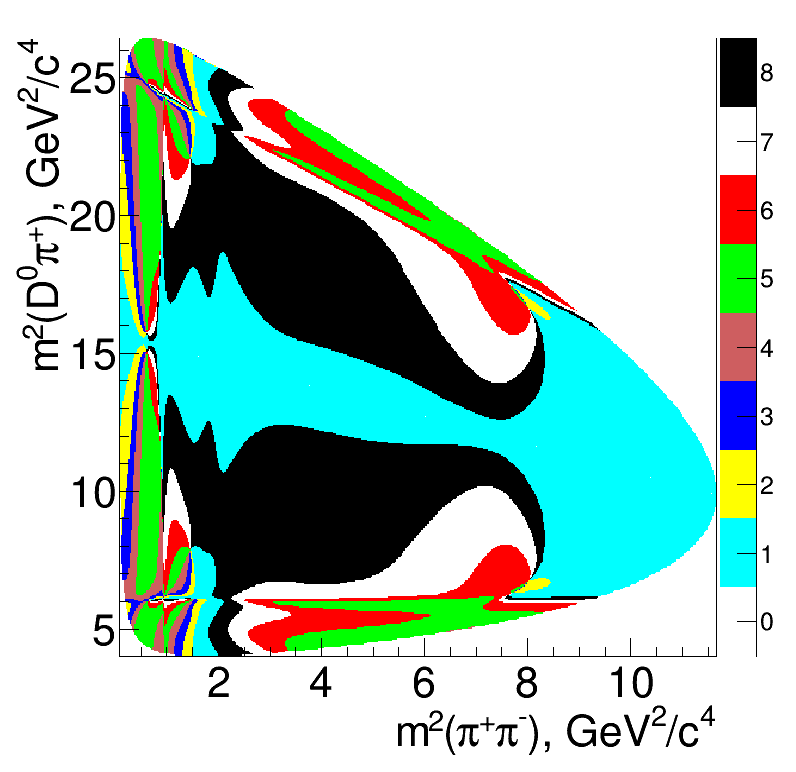
\includegraphics[width=0.8\textwidth]{d0pipi_binning2_rotated}
 \subcaption{}
 \label{fig:bdbpp-bins}
\end{minipage}
\begin{minipage}[b]{0.5\textwidth}
 \centering
  \includegraphics[width=0.8\textwidth]{CS_bdpp_v4}
 \subcaption{}
 \label{fig:csj}
\end{minipage}
 \caption{а) Равномерное по фазе разбиение диаграммы Далица распада \bdbpp, полученное на основе упрощенной версии модели, опубликованной в работе~\cite{kuzmin_model}, и б) значения параметров $c_j$ и $s_j$, полученные с помощью этой модели, (синие круги).  Красные квадраты показывают пример измерения и ожидаемую точность при измерении параметров $c_j$ и $s_j$ в эксперименте \belleii.}
 \label{fig:bdbpp}
\end{figure}

Полученные значения параметров $k_j$, $c_j$ и $s_j$ использованы для генерирования событий в соответствии с оценками из таблицы~\ref{tab:yield}.  Сгенерированные события использовались для определения величин параметров \pphi, $c_j$ и $s_j$ методом максимального правдоподобия.  Полученные значения статистической неопределенности для параметра \pphi приведены в таблице~\ref{tab:precision}.  На рисунке~\ref{fig:csj} показан результат определения величины параметров $c_j$ и $s_j$, соответствующий размеру выборки, ожидаемому в эксперименте \belleii.

\begin{table}[H]
 \centering
 \caption{Результаты численных экспериментов: статистическая неопределенность при модельно-независимом измерении параметра \pphi в распадах \bdbpp и \bdsth с последующими переходами $D$-мезона в \cpconj-собственные состояния и состояние \kspp.  Результаты были получены для значения параметра $\pphi=23\grad$.}
 \label{tab:precision}
\begin{tabular}{lcc}
 \hline\hline
 \multirow{2}{*}{Тип событий}& \multicolumn{2}{c}{$\delta\pphi$ (град.)} \\
                          & \belle          & \belleii \\% & LHCb (RI) & LHCb (RII) & LHCb (Upg)\\
 \hline
 \bdbpp                   & $ 7.6\grad$ & $1.2\grad$\\ % & $8.2\grad$ & $7.7\grad$ & $1.9\grad$ \\
 \bdbpp (симм. области)   & $10\grad$   & $1.5\grad$\\ % & $16\grad$  & $10\grad$ & $2.7\grad$ \\
 \bdsth                   & $ 4.4\grad$ & $0.7\grad$\\ % & --- & --- & --- \\
 \hline\hline
 \end{tabular}
\end{table}

Полученные результаты позволяют сделать несколько выводов.  Точность модельно-независимого измерения параметра \pphi в распадах \bdbpp примерно в~$1.5$ раз хуже, чем в распадах~\bdsth.  Симметризация областей на диаграмме Далица распада \bdbpp приводит к значительному уменьшению статистической чувствительности метода; эта модификация может быть выбрана только из соображений сложных фоновых условий в конкретном измерении.  
Можно ожидать, что данные эксперимента \belleii позволят выполнить модельно-независимое измерение параметра \pphi в переходах \btocud с точностью лучше~$1\grad$.  Этот результат будет служить важным инструментом для проверки механизма \km и ограничения вкладов НФ.

\section{Разбиение фазового пространства в пределе большой статистики}\label{sec:big-data}
Завершая обсуждение модельно-независимого подхода к анализу многочастичных распадов, кратко рассмотрим вопрос об оптимизации разбиения фазового пространства в условиях большого количества экспериментальных данных.  В работах~\cite{Bondar2008,CLEO_phases} рассматривался вопрос об оптимизации формы областей при заданном их количестве $2\mcn$.  Процедуры оптимизации, предложенные в этих работах, основаны на использовании модели распада и дают желаемый результат только при условии адекватности модели.

Более прямолинейный путь приближения к предельной статистической чувствительности метода состоит в увеличении количества областей, на которые разбивается фазовое пространство распада \dnkpp.  При этом, количество областей разумно увеличивать только до тех пор, пока размер области больше или порядка экспериментального разрешения для переменных Далица (которое для $B$-фабрик близко к $2\times 10^{-3}\gev^{2}/c^{4}$).  Этот предел приблизительно соответствует $4\times 10^5$ областям.  Учитывая, что на Супер-Чарм-Тау-фабрике со светимостью $10^{35}\lumi$ число событий с распадом обоих $D$-мезонов в \kspp может достигать $10^6$ событий, число областей фазового пространства может достигать нескольких тысяч.

При $\mcn\gtrsim 100$ могут возникнуть сложности вычислительного характера, поскольку при измерении параметров \ci и \si необходимо решать систему из $\mcn^2$ нелинейных уравнений относительно $2\mcn$ неизвестных (смотрите пункт~\ref{sec:cs_measurement}).  Одна из возможных процедур, свободная от сложностей такого рода, состоит в измерении параметров \ci и \si в два этапа.  На первом этапе реализуется описанная в пункте~\ref{sec:cs_measurement} процедура для небольшого $\mcn_0$, например, равного $8$.  Затем, при анализе когерентных  распадов $\ep\to(\kspp)_D(\kspp)_D$, для одной из диаграмм Далица используется $\mcn_0$, а для другой --- большое \mcn.  При такой процедуре система уравнений разбивается на $\mcn$ независимых систем, каждая из которых содержит $4\mcn_0$ уравнений ($2\mcn_0$ уравнений для каждой пары симметричных областей мелкого разбиения и двух неизвестных параметров~\ci и~\si).

При наличии Супер-Чарм-Тау-фабрики, вероятно, статистическая точность определения параметра \gphi будет определяться числом событий \bdk, \dkpp в экспериментах \belleii и \lhcb (можно ожидать порядка $10^5$ событий).  Максимальное число областей фазового пространства распада \dnkpp при этом может достигать нескольких тысяч, а экспериментальное разрешение для переменных Далица еще не будет ограничивающим фактором.

Можно ожидать, что при разбиении фазового пространства на $10^3$ и более областей, форма каждой области уже не будет иметь существенного значения, а статистическая точность метода будет близка к точности модельно-зависимого измерения.
%Помимо этого, остается открытым вопрос о существовании правила разбиения фазового пространства, которое в общем случае приводило бы к лучшей статистической чувствительности, чем правило~\eqref{eq:uniph}.  


             % Глава 2
\chapter{Эксперимент Belle} \label{sec:belle-exp}
\section{Ускоритель KEKB} \label{sec:kekb}
Ускоритель \kekb --- это асимметричный \ep-коллайдер с энергией в \cms $\sqrt{s}=10.58\gev$, соответствующей массе резонанса~\ups, разработанный для рождения большого количества \bbbar-пар.  Ускоритель введен в эксплуатацию в 1998 году и состоит из двух накопительных колец периметром примерно $3~\textrm{км}$, находящихся в $11\textrm{м}$ под землей (рисунок~\ref{fig:KEKB}).  Электроны и позитроны ускоряются до энергий $8\gev$ и $3.5\gev$, соответственно.  Пучки электронов и позитронов циркулируют в соответствующих накопительных кольцах и пересекаются в единственном месте взаимодействия под углом $11~\textrm{мрад}$.
\begin{figure}[htb]
 \centering
  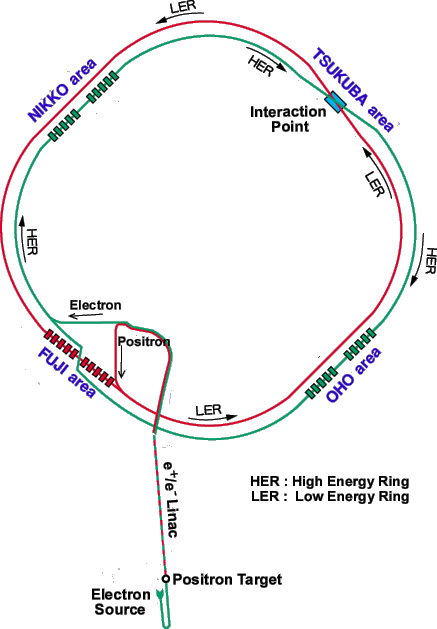
\includegraphics[width=0.5\textwidth]{KEKB}
  \caption{Ускоритель \kekb.}
\label{fig:KEKB}
\end{figure}

Разность энергий пучков ускорителя \kekb соответствует Лоренц-фактору $\bg_{\ups}=0.425$ в лабораторной системе отсчета.  Начальный импульс $B$-мезонов приводит к доступному для измерения пространственному разделению вершин распада двух рожденных $B$-мезонов, равному примерно $200\mum$. При симметричном рождении пространственное разделение составляло бы примерно $30\mum$.

Ускоритель \kekb разрабатывался для достижения светимости $\mcl=1.0\times 10^{34}\lumi$, соответствующей рождению десяти \bbbar-пар в секунду.  В течение работы, ускоритель был существенно модернизирован.  В частности, оснащен технологией crab cavities, увеличивающий светимость за счет поворота пучков в вблизи области взаимодействия.  Эти усилия позволили превзойти многие заложенные при проектировании параметры, достичь рекордной светимости $\mcl=2.1\times 10^{34}\lumi$.

Детектор \belle набрал интеграл светимости $711\ifb$, соответствующий $772\times10^6$ \bbbar-парам, рожденным на ускорителе \kekb, работающем вблизи резонанса \ups.  Кроме того, ускоритель \kekb работал при других энергиях.  В частности, детектор Belle набрал интеграл светимости $121\ifb$ на резонансе $\Upsilon(5S)$, что позволяет проводить измерения в системе $B_s$-мезонов, а также изучать спектроскопию $b\overline{b}$-состояний.  Полный интеграл светимости, набранный детектором Belle на ускорителе \kekb превышает~$1~\textrm{абн}^{-1}$ (рисунок~\ref{fig:KEKB-lum}).

\begin{figure}[htb]
 \centering
  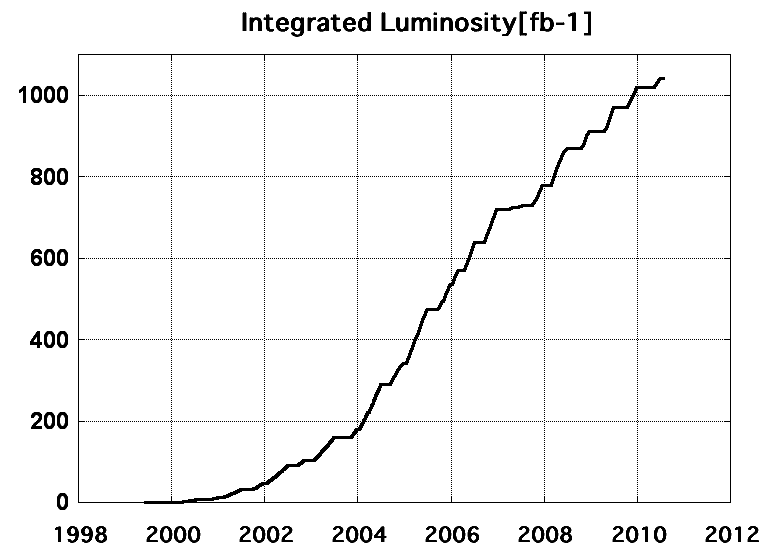
\includegraphics[width=0.5\textwidth]{KEKB-luminosity-bw.png}
  \caption{Интеграл светимости, набранный детектором \belle на ускорителе \kekb.}
\label{fig:KEKB-lum}
\end{figure}

Детальное описание ускорителя \kekb приведено в работах~\cite{KEKB1,KEKB2}.

\clearpage
\section{Детектор Belle}\label{sec:belle}
Детектор $\belle$ --- это универсальный детектор, охватывающий близкий к $4\pi$ телесный угол вокруг области взаимодействия пучков.  Детектор оптимизирован для выполнения времязависимых  измерений и работе с асимметричным \ep-коллайдером \kekb.  Схема детектора приведена на рисунке~\ref{fig:Belle}.  

\begin{figure}[htb]
 \centering
  \includegraphics[width=\textwidth]{BelleDetector}
  \caption{Детектор \belle.}
\label{fig:Belle}
\end{figure}

Детектор \belle оборудован сверхпроводящим магнитом, создающим магнитное поле $1.5~\textrm{Тл}$, и несколькими подсистемами для регистрации и идентификации заряженных и нейтральных частиц.  Треки заряженных частиц реконструируются на основе измерений кремниевого вершинного детектора (\svd) и центральной дрейфовой камеры (\cdc).  Электромагнитные ливни регистрируются кристаллами \csit электромагнитного калориметра (\ecl).  Кристаллы \textrm{BGO} переднего калориметра малых углов закрывают трубу ускорителя, уменьшая фон для \cdc, и используются в качестве монитора светимости.  Мюоны и $K_L^0$-мезоны регистрируются счетчиками, помещенными в железное ярмо, замыкающее магнитный поток.  Помимо измерения потери энергии в \cdc, идентификация частиц производится с помощью измерений аэрогелевых пороговых черенковских счетчиков и времяпролетных счетчиков, расположенных за пределами \cdc.



Расположение и принципы работы некоторых подсистем детектора \belle кратко описаны в следующих пунктах.  Описания следуют техническим публикациям, ссылки на которые приведены, и в которых может быть найдена более полная информация.  Для анализа данных с детектора \belle, описанного в главе~\ref{sec:bdsth}, важны: трековая система, электромагнитный калориметр и системы идентификации частиц.

%\subsection{Труба ускорителя}\label{sec:beam-pipe}
\subsection{Кремниевый вершинный детектор}\label{sec:svd}
Основной целью эксперимента \belle является наблюдение времязависимого нарушения \cpconj-нарушения в распадах нейтральных $B$-мезонов.  Для таких анализов необходимо прецизионное измерение расстояния между вершинами распадов двух $B$-мезонов, рожденных при распаде резонанса \ups.  В разделе~\ref{sec:kekb} обсуждалось, что характерное расстояние между вершинами составляет примерно $200\mum$.  Необходимо, таким образом, чтобы кремниевый вершинный детектор (\svd) обладал высоким пространственным разрешением и был способен определить $z$-координату трека с точностью около $100\mum$.

\svd является ближайшим к области взаимодействия пучков детектором.  Он расположен вблизи бериллиевой трубы ускорителя.  Этот детектор должен быть устойчив к большим дозам облучения, обусловленным пучковым фоном.  \svd разделен на слои различных радиусов вокруг трубы ускорителя.  В каждом слое установлены пластины двусторонних кремниевых полосковых детекторов (\dssd).  \dssd содержат обедненные $pn$-переходы.  Проходя сквозь обедненные $pn$-переходы, заряженные частицы создают электрон-дырочные пары вдоль своей траектории.  Электроны и дырки дрейфуют, соответственно, к $n$- и $p$-полоскам на поверхности \dssd.  $n$-полоски расположены перпендикулярно, а $p$-полоски расположены вдоль оси пучков.  Таким образом обеспечивается измерение координат траектории вдоль направлений $r\varphi$ и $z$, соответственно.

Два разных вершинных детектора работали в эксперименте \belle.  Первоначальный \svd, который мы будем называть $\svd1$, работал с $1999$ по $2003$ годы.  Детектор $\svd1$ имеет цилиндрическую структуру и состоит из трех слоев с радиусами $30\mm$, $45.5\mm$ и $60.5\mm$.  Он охватывает диапазон полярных углов от $23\grad$ до $139\grad$, что соответствует $86\%$ полного телесного угла.  $\svd1$ состоит из $102$ \dssd.  Каждый \dssd имеет $1280$ чувствительных полосок и по $640$ считывающих каналов на противоположных сторонах.  Пространственный период полосок составляет $42\mum$ в направлении $z$ и $25\mum$ в направлении $\varphi$.  Площадь активной зоны \dssd составляет приблизительно $55\times 33\mm^{2}$.

\svd был модернизирован в $2003$ году.  Модернизированную версию \svd мы будем называть $\svd2$.  $\svd2$ расположен ближе к трубе ускорителя и покрывает больший диапазон полярных углов $\theta$.  Расположение частей $\svd2$ показано на рисунке~\ref{fig:svd}.  Он состоит из четырех слоев радиусами $20\mm$, $43.5\mm$, $70\mm$ и $88\mm$ и покрывает диапазон полярных углов от $17\grad$ до $150\grad$, что соответствует $93\%$ полного телесного угла.  $\svd2$ состоит из $246$ \dssd.  Используются два типа \dssd с пространственным периодом полосок от $50\mum$ до $75\mum$.  Площадь активно зоны \dssd в первых трех слоях составляет $28.4\times 79.6\mm^{2}$, а в четвертом слое --- $34.9\times 76.4\mm^{2}$.

% \begin{figure}[H]
%  \centering
%  \begin{minipage}{0.49\textwidth}
%  \centering
%  \vspace{0.9 cm}
%   \includegraphics[width=0.7\textwidth]{svd1}
%   \subcaption{}
%   \label{fig:svd1}
%  \end{minipage}
%  \begin{minipage}{0.49\textwidth}
%   \centering
%   \includegraphics[width=0.9\textwidth]{svd2}
%   \subcaption{}
%   \label{fig:svd2}
%  \end{minipage}
%   \\
%   \begin{minipage}{0.8\textwidth}
%   \includegraphics[width=\textwidth]{svd_front_v2}
%   \subcaption{}
%   \label{fig:svd2-front}
%  \end{minipage}
%   \caption{Расположение чувствительных полосок а) $\svd1$ и б) $\svd2$ и в) схема расположения $\svd2$.}
% \label{fig:svd}
% \end{figure}

Количественной характеристикой работы \svd является разрешение при измерении прицельного параметра трека.  Прицельным параметром заряженного трека называется наименьшее расстояние до точки взаимодействия пучков.  Разрешение при измерении прицельного параметра может отличаться для \rphi- и $z$-направлений, а также может зависеть от импульса и полярного угла $\theta$ частицы.  Разрешение в \rphi- и $z$-направлениях может быть описано следующими функциями:
\begin{equation}
\begin{split}
 &\sigma^{1}_{\rphi} = 19.2\mum \oplus \frac{54.0\mum}{p\beta\sin^{3/2}\theta},\quad
  \sigma^{1}_{z}     = 42.2\mum \oplus \frac{44.3\mum}{p\beta\sin^{5/2}\theta},\\
 &\sigma^{2}_{\rphi} = 21.9\mum \oplus \frac{35.5\mum}{p\beta\sin^{3/2}\theta},\quad
  \sigma^{2}_{z}     = 27.8\mum \oplus \frac{31.9\mum}{p\beta\sin^{5/2}\theta}, 
\end{split}
\end{equation}
где символ $\oplus$ обозначает квадратичное сложение, индексы $1$ и $2$ соответствуют $\svd1$ и $\svd2$ и импульс $p$ выражен в\gevc (смотрите рисунок~\ref{fig:svd-resolution}).  Детальное описание \svd приведено в работах~\cite{svd1,svd2}.

\begin{figure}[H]
 \centering
 \begin{minipage}{0.39\textwidth} 
 \begin{subfigure}{\linewidth}
 \centering
  \includegraphics[width=0.7\textwidth]{svd1}
  \subcaption{}
  \label{fig:svd1}
 \end{subfigure}\\ \vspace{0.1 cm}
 
 \begin{subfigure}{\linewidth}
  \centering
  \includegraphics[width=0.9\textwidth]{svd2}
  \subcaption{}
  \label{fig:svd2}
 \end{subfigure}
% \vspace{0.9 cm}
 \end{minipage}
 \begin{minipage}{0.59\textwidth}
  \includegraphics[width=\textwidth]{svd-resolution-16bit}
  \subcaption{}
  \label{fig:svd-resolution}
 \end{minipage}
  \\
  \begin{minipage}{0.8\textwidth}
  \includegraphics[width=\textwidth]{svd_front_v2}
  \subcaption{}
  \label{fig:svd2-front}
 \end{minipage}
  \caption{Схемы расположения чувствительных полосок а)~$\svd1$ и б)~$\svd2$; в)~разрешение по прицельному параметру трека в зависимости от импульса частицы; г)~схема расположения $\svd2$.}
\label{fig:svd}
\end{figure}

% [78] Y. Ushiroda. “Belle Silicon Vertex Detectors”. Nuclear Instruments and Methods A, 511
% (1–2):6–10, 2003. Proceedings of the 11th International Workshop on Vertex Detectors.
% [79] Z. Natkaniec, H. Aihara, Y. Asano et al. “Status of the Belle Silicon Vertex Detector”.
% Nuclear Instruments and Methods A, 560(1):1–4, 2006.
% [80] M. Fujikawa. “Measurement of Branching Fraction and Time-dependent CP Asymme-
% try Parameters in B0 → K0 π0 Decays”. PhD thesis, Nara Women’s University, 2009.

%\subsection{Калориметр малых углов}\label{sec:efc}

\subsection{Центральная дрейфовая камера}\label{sec:cdc}
Центральная дрейфовая камера (\cdc) разработана для реконструкции треков заряженных частиц.  \cdc расположена внутри магнитного поля $1.5~\textrm{Тл}$, создаваемого сверхпроводящим магнитом, что позволяет определять импульс заряженных частиц, используя кривизну восстановленных треков.  Кроме того, \cdc используется для измерения энергетических потерь заряженных частиц ($\dd E/\dd x$), которые используется для идентификации частиц.  Информация от \cdc также используется в системе триггера.

\cdc~--- это цилиндрическая проволочная дрейфовая камера, состоящая из $50$ слоев анодных проволочек и трех слоев катодных полосок.  Длина \cdc составляет $2404\mm$, внутренний и внешний радиусы равны $83\mm$ и $888\mm$.  Расположение \cdc показано на рисунке~\ref{fig:cdc}.  Чтобы учесть асимметрию энергий пучков, \cdc асимметрична в направлении $z$ и покрывает диапазон полярных углов от $17\grad$ до $150\grad$, что соответствует $92\%$ полного телесного угла.  \cdc состоит из $8400$ дрейфовых ячеек, организованных в $6$ аксиальных и $5$ стерео слоев.  Каждый стерео слой содержит от $3$ до $6$ радиальных слоев с одинаковым количеством дрейфовых ячеек в азимутальном направлении.  Дрейфовые ячейки состоят из $8$ проволочек с отрицательным потенциалом, обеспечивающих электрическое поле вокруг проволочки с положительным потенциалом.  Структура ячейки и расположение проволочек показаны на рисунке~\ref{fig:cdc-cell}

\cdc наполнен газовой смесью, состоящей на $50\%$ из гелия и на $50\%$ из этана.  Смесь из газов с небольшой атомной массой $Z$ минимизирует влияние множественного кулоновского рассеяния, особенно для частиц с небольшим импульсом, и уменьшает фон от синхротронного излучения благодаря малости сечения фотоэффекта.  Кроме того, этановая компонента обеспечивает хорошее разрешение по \dedx.

Проходя через дрейфовые ячейки, заряженные частицы ионизируют газ вдоль своей траектории.  Образовавшиеся ионы и свободные электроны дрейфуют, соответственно, к катодным и анодным проволочкам.  В сильном электрическом поле анодных проволочек происходит усиление электрического сигнала, регистрируемого чувствительными проволочками.  Проволочки в аксиальных слоях позволяют измерить поперечный импульс \pt, в то время как стерео слои, установленные с малым углом, дают дополнительную информацию для измерения продольной компоненты импульса \pl.  Детальное описания алгоритма восстановления трека и определения импульса приведено в работе~\cite{cdc}.

\begin{figure}[h]
 \centering
  \includegraphics[angle=270,width=\textwidth]{cdcfig_01}\\
  \caption{Схема расположения центральной дрейфовой камеры детектора \belle~\cite{BelleNIM}.}
\label{fig:cdc}
\end{figure}

\begin{figure}[H]
 \centering
\includegraphics[width=0.35\textwidth]{cdcfig_02}\hfill
\includegraphics[width=0.5\textwidth]{cdcfig_03}
  \caption{Схема расположения проволочек в центральной дрейфовой камере детектора \belle~\cite{BelleNIM}.}
\label{fig:cdc-cell}
\end{figure}

Разрешение по поперечному импульсу в \cdc описывается функцией
\begin{equation}
 \left.\frac{\sigma_{\pt}}{\pt}\right|_{\cdc} = \left(0.28\pt\oplus\frac{0.35}{\beta}\right)\%,
\end{equation}
где $\pt$ обозначает величину поперечного импульса трека в\gevc и $\beta$ обозначает скорость частицы в единицах скорости света.  При комбинировании информации с \cdc и \svd, разрешение по \pt улучшается:
\begin{equation}
 \left.\frac{\sigma_{\pt}}{\pt}\right|_{\cdc+\svd} = \left(0.19\pt\oplus\frac{0.30}{\beta}\right)\%.
\end{equation}

Амплитуды сигналов сработавших проволочек используются для измерения потери энергии (\dedx) заряженной частицы в \cdc.  Величина потерь \dedx подчиняется формуле Блоха и зависит от скорости частицы.  Скорость при данном импульсе зависит от массы частицы и, значит, измерение \dedx может быть использовано для идентификации заряженных частиц.  Измеренные значения \dedx подчиняются распределению Ландау с широкими хвостами, поэтому для оценки наиболее вероятного измеренного значения \dedx применяется метод усеченного среднего, позволяющий минимизировать вклад больших флуктуаций.  Зависимость \dedx от импульса частицы приведена на рисунке~\ref{fig:dedx}.

Детальное описание \cdc содержится в работах~\cite{BelleNIM,cdc}.

\begin{figure}[H]
 \centering
 \includegraphics[width=0.8\textwidth]{cdcfig_dEdx}\\
  \caption{Зависимость ионизационных потерь от импульса частиц.  Точками показаны экспериментальные данные, линиями --- ожидаемые энергетические потери для различных типов частиц~\cite{BelleNIM}.}
\label{fig:dedx}
\end{figure}

%[cdc1] [81] Belle Tracking Group. “Charged Particle Tracking at Belle”. Belle Note #327, 2000.
%[cdc2] [82] H. Hirano, M. Akatsu, Y. Fujita et al. “A High-resolution Cylindrical Drift Chamber for the KEK B-Factory”. Nuclear Instruments and Methods A, 455(2):294–304, 2000.

\subsection{Аэрогелевые черенковские счетчики}
Аэрогелевый черенковский счетчик (\acc) --- это детектор для идентификации частиц, в данном случае для разделения заряженных $\pi$- и $K$-мезонов.  Он обладает разделительной способностью в диапазоне импульсов заряженных частиц от $1\gevc$ до $4\gevc$, расширяя диапазон, в котором применима идентификация по $\dd E/\dd x$ и по информации от времяпролетных счетчиков.

Заряженные частицы, пролетающие сквозь среду со скоростью, превышающей скорость распространения света в этой среде, излучают свет, называемый черенковским излучением.  Условие, при котором возникает черенковское излучение, зависит от показателя преломления среды следующим образом:
\begin{equation}
 n>\frac{1}{\beta}=\sqrt{1+\left(\frac{m}{p}\right)^2},
\end{equation}
где $\beta$ --- скорость частицы и $n$ --- показатель преломления среды.  Материал среды в \acc выбран таким, чтобы $\pi$-мезоны с импульсом больше $1\gevc$ производили черенковское излучение, но чтобы скорость более тяжелых заряженных $K$-мезонов с тем же импульсом была под порогом генерации черенковского излучения.  \acc работает только как пороговый счетчик, не измеряя черенковский угол, зависящий от скорости частицы,  и который также может быть использован для идентификации частиц.

\acc разделен на цилиндрическую и торцевую части, которые покрывают полярный угол от $17\grad$ до $127\grad$.  Цилиндрическая часть детектора состоит из $960$ счетчиков, сгруппированных в $60$ ячеек в $\varphi$-направлении.  Торцевая часть детектора состоит из $228$ счетчиков, сгруппированных в $5$ концентрических слоя.  Счетчики направлены в место встречи пучков.  Расположение счетчиков показано на рисунке~\ref{fig:acc}.  Каждый счетчик состоит из слоя кварцевого аэрогеля, расположенного в алюминиевом корпусе размером $12\times12\times12\cm^{3}$.  Коэффициент преломления кварцевого аэрогеля находится в диапазоне от $1.010$ до $1.030$ и зависит от полярного угла.  Черенковский свет регистрируется сеточными фотоумножителями, закрепленными в алюминиевых корпусах.

Используя только сигналы с \acc, можно идентифицировать заряженные $K$-мезоны с импульсами до $4\gevc$ с эффективностью больше $80\%$ при соответствующей ошибочной $\pi$-мезонной идентификацией меньше $10\%$.

Детальное описание \acc содержится в работах~\cite{BelleNIM,acc}.

\begin{figure}[H]
 \centering
 \includegraphics[width=\textwidth]{ACC_det_clean}\\
  \caption{Расположение аэрогелевых черенковских и времяпролетных счетчиков детектора \belle~\cite{BelleNIM}.}
\label{fig:acc}
\end{figure}

%[acc] [83] T. Iijima, I. Adachi, R. Enomoto et al. “Aerogel Cherenkov Counter for the Belle De-
%tector”. Nuclear Instruments and Methods A, 453(1):321–325, 2000.

\subsection{Времяпролетные счетчики}
Система времяпролетных счетчиков (\tof) измеряет время, за которое частица прошла расстояние от места встречи до \tof.  Сопоставляя результаты измерения с измеренным импульсом, можно получить полезную для идентификации частицы информацию, в частности, для разделения заряженных $\pi$- и $K$-мезонов.  \tof обладают достаточной разрешающей способностью для заряженных частиц с импульсом меньше $1.2\gevc$.  Таким образом, система \tof является комплиментарной к системе \acc.  Кроме  того, система \tof генерирует быстрые временные сигналы для триггерной системы.

\begin{figure}[htb]
 \centering
 \includegraphics[width=\textwidth]{toffig1}\\
  \caption{Расположение времяпролетных счетчиков детектора \belle~\cite{BelleNIM}.}
\label{fig:tof}
\end{figure}

\tof состоят из пластиковых сцинтилляционных пластин, присоединенных к сеточным фотоумножителям и расположенных в цилиндрической части детектора (рисунок~\ref{fig:tof}).  Радиальное расстояние до места встречи составляет $1.2~\textrm{м}$.  \tof покрывают полярный угол в диапазоне от $34\grad$ до $120\grad$ и обладают временным разрешением около $100\ps$.

Масса частицы соотносится с измеренным временем пролета $T$ следующим образом:
\begin{equation}
 m = \frac{p}{c}\sqrt{\left(\frac{cT}{L}\right)^2-1},
\end{equation}
где $p$ обозначает импульс частицы, измеренный в \cdc и \svd и $L$ обозначает расстояние, которое частица прошла по спиральной траектории от места встречи до \tof.  Распределение по массе, полученное с помощью измерений в системе \tof с использованием импульса, измеренного в \cdc, для адронных событий, показано на рисунке~\ref{fig:tof-id}.

\begin{figure}[htb]
 \centering
 \includegraphics[width=0.6\textwidth]{toffig12}\\
  \caption{Распределение масс частиц, полученное с помощью измерения времени пролета~\cite{BelleNIM}.  Гистограмма показывает результаты моделирования, точками обозначены экспериментальные результаты.}
\label{fig:tof-id}
\end{figure}

Детальное описание \tof содержится в работах~\cite{BelleNIM,tof}.

%[tof] [84] H. Kichimi, Y. Yoshimura, T. Browder et al. “The Belle TOF System”. Nuclear Instru-
%ments and Methods A, 453(1):315–320, 2000.

\subsection{Электромагнитный калориметр}
Электромагнитный калориметр (\ecl) измеряет энергию и координату электромагнитных ливней, порожденных фотонами и электронами.  Электромагнитные ливни развиваются в результате каскадного рождения \ep-пар и испускания фотонов в поле ядра атома.  \ecl должен обеспечивать высокое энергетическое разрешение в широком динамическом диапазоне от $20\mevcsq$ до $8\gevcsq$.  Это требование обусловлено необходимостью регистрации низкоэнергетичных фотонов, например, из распадов \pin- и $\eta$-мезонов, и высокоэнергетичных фотонов из распадов $B$-мезонов, таких как $\bn\to K^{*0}\gamma$.  Кроме того, \ecl используется для измерения светимости и калибровок с использованием событий Баба-рассеяния ($\ep\to\ep$) и процессов $\ep\to\gamma\gamma$.

\ecl состоит из сегментированного набора счетчиков, собранного из $8376$ сцинтилляционных кристаллов йодида цезия, активированных талием (\csit).  Считывание сигнала с каждого кристалла производится с помощью двух PIN-фотодиодов.   В цилиндрической части \ecl расположены $6624$ кристалла.  В передней и задней торцевых частях расположены, соответственно, $1152$ и $960$ кристаллов.  \ecl покрывает полярный угол в диапазоне от $12\grad$ до $155\grad$.  Кристаллы расположены под небольшим наклоном, от $1.3\grad$ до $4.0\grad$ в $\varphi$- и $\theta$-направлениях для предотвращения пролета фотонов в пространстве между кристаллами.  Расположение кристаллов \ecl показано на рисунке~\ref{fig:ecl}.

\begin{figure}[htb]
 \centering
 \includegraphics[angle=-90,width=\textwidth]{csi_overall_conf}\\
  \caption{Схема электромагнитного калориметра детектора \belle~\cite{BelleNIM}.}
\label{fig:ecl}
\end{figure}

Кристаллы \csit, расположенные в цилиндрической части, имеют переднюю и заднюю поверхность, соответственно, $5.5\cm\times 5.5\cm$ и $6.5\cm\times 6.5\cm$, и длину $30\cm$, соответствующую $16.2$ радиационным длинам.  Кристаллы в торцевых частях имеют передние и задние поверхности с размерами сторон от $4.5\cm$ до $8.2\cm$.  Размеры кристаллов выбраны таким образом, чтобы приблизительно $80\%$ энергии фотона, попавшего в центр передней поверхности кристалла, высадилась в этом кристалле.

Энергетическое разрешение \ecl описывается функцией
\begin{equation}
 \frac{\sigma_E}{E}=\left(1.34\oplus\frac{0.066}{E}\oplus\frac{0.81}{E^{1/4}} \right)\%,
\end{equation}
где энергия $E$ выражена в\gev.  Энергетическое разрешение ограничено шумом электроники, дающим вклад в первое слагаемое, и флуктуациями утечек ливней, дающими второе и третье слагаемые.

\begin{figure}[htb]
 \centering
 \begin{minipage}[b]{0.45\textwidth}
 \centering
  \includegraphics[width=0.99\textwidth]{pi0}
 \subcaption{}
 \label{fig:ecl-pi0}
\end{minipage}
\begin{minipage}[b]{0.45\textwidth}
 \centering
  \includegraphics[width=0.99\textwidth]{eta}
 \subcaption{}
 \label{fig:ecl-eta}
\end{minipage}
  \caption{Двухфотонные спектры в вблизи масс а)~\pin-мезона и б)~$\eta$-мезона~\cite{BelleNIM}.  Гистограммы показывают результаты моделирования, точками обозначены экспериментальные результаты.}
\label{fig:ecl-resolution}
\end{figure}

На рисунке~\ref{fig:ecl-resolution} показаны экспериментальные двухфотонные массовые спектры в области масс \pin- и $\eta$-мезонов, полученные с помощью адронных событий.  Массовое разрешение для \pin- и $\eta$-мезонов составляет приблизительно $5\mevcsq$ и $12\mevcsq$, соответственно.

Кроме измерения энергии, \ecl дает информацию для идентификации электронов.  Заряженные $K$- и $\pi$-мезоны можно отличить от электронов по форме ливня, описанной отношением энерговыделений $E_9/E_{25}$, измеренных в матрицах кристаллов $3\times3$ и $5\times5$, соответственно, и отношением энерговыделения к импульсу $E/p$, которое близко к единице для электронов и мало для остальных частиц.

Детальное описание \ecl содержится в работах~\cite{BelleNIM,ecl}.

%[85] K. Miyabayashi. “Belle Electromagnetic Calorimeter”. Nuclear Instruments and Me-
%thods A, 494(1):298–302, 2002.

\subsection{Сверхпроводящий магнит}\label{sec:magnet}
Сверхпроводящий магнит создает магнитное поле величиной $1.5~\textrm{Тл}$ в цилиндрическом объеме диаметром $3.4~\textrm{м}$ и длиной $4.4~\textrm{м}$.  Он охватывает все компоненты детектора, кроме мюонной системы, которая расположена за магнитом в ярме детектора \belle.  Железное ярмо также служит для замыкания магнитного потока.

\begin{figure}[htb]
 \centering
 \includegraphics[width=0.8\textwidth]{coil}
  \caption{Схема сверхпроводящего магнита детектора \belle~\cite{BelleNIM}.}
\label{fig:magnet}
\end{figure}

Сверхпроводящая катушка состоит из ниобий-титан-медного (\textrm{NbTi/Cu}) кабеля, стабилизированного алюминием и охлаждаемого жидким гелием.  Проводник имеет сечение $3\mm\times 33\mm$.  Катушка рассчитана на номинальный ток $4400~\textrm{А}$ и запасенную энергию $35\mdz$.  Вид сверхпроводящего магнита и сечение катушки показаны на рисунке~\ref{fig:magnet}.

Детальное описание сверхпроводящего магнита содержится в работе~\cite{BelleNIM}.

%\subsection{Детектор мюонов и $K_L^0$-мезонов}

%\clearpage
\section{Триггер и система сбора данных}
Сбор и хранение данных, набираемых детектором \belle, контролируются триггерной системой.  Используя быстрые сигналы от разных частей детектора, триггерная система принимает решение о том, интересно ли событие с точки зрения физики (в этом случае событие обрабатывается системой сбора данных (\daq) и записывается для последующего анализа) или его следует пропустить.  В качестве примера интересных для анализа событий можно привести следующие:
\begin{itemize}
 \item Адронные распады \ups или адронные события из \qqbar-континуума;
 \item События, содержащие пары $\mu$- и $\tau$-лептонов;
 \item События Баба-рассеяния или двухфотонные процессы.
\end{itemize}
Примеры событий, которые при нормальной работе пропускаются:
\begin{itemize}
 \item Фоновые события, связанные с пучками частиц, например, обусловленные синхротронным излучением или взаимодействием пучка с остаточным газом в трубе ускорителя;
 \item Фоновые события, порожденные космическими лучами.
\end{itemize}

В таблице~\ref{tab:rates} приведены сечения и частоты физических процессов при светимости $\mcl=1.0\times 10^{34}\lumi$.  Суммарная частота физических процессов составляет приблизительно $100\gz$ при этой светимости.  Частота пучкового фона составляет порядка $120\gz$ и зависит от состояния ускорителя, приводя к полной частоте около $220\gz$.  При светимости ускорителя \kekb, равной $\mcl=2\times 10^{34}\lumi$, частота физических и фоновых процессов возрастает до $200\gz$ и $600\gz$, соответственно.  Триггерная система способна обработать события, поступающие с частотой до $1200\gz$ и допускает срабатывание триггера с частотой до $500\gz$.

\begin{table}[htb]
%\begin{small}
  \caption{Сечения и частоты для различных процессов \ep-ускорителя \kekb, работающего вблизи \ups-резонанса со светимостью $\mcl=1.0\times 10^{34}\lumi$.  Символом $*$ отмечены значения, которые на триггерном уровне масштабируются с коэффициентом $100$.}
 \label{tab:rates}
 \begin{tabular}
  { @{\hspace{0.3cm}}l@{\hspace{0.3cm}}  @{\hspace{0.3cm}}c@{\hspace{0.3cm}} @{\hspace{0.3cm}}c@{\hspace{0.3cm}} }
  \hline\hline
 Процесс  &  Сечение (\textrm{нбн})  & Частота (\textrm{Гц}) \\ \hline
  $\ups\to\bbbar$                                 & $1.2$ & $12$ \\
  $\ep\to\qqbar$ ($q\in\{u,d,s,c\}$) континуум    & $2.8$ & $28$ \\
  $\ep\to l^+l^-$ ($l\in\{\mu,\tau\}$) континуум  & $1.6$ & $16$ \\
  Баба-рассеяние ($\theta_{\lab}>17\grad$)        & $44$  & $4.4^{*}$ \\
  $\ep\to\gamma\gamma$ ($\theta_{\lab}>17\grad$)  & $2.4$ & $0.24^{*}$ \\
  Процессы $2\gamma$ ($\theta_{\lab}>17\grad$, $\pt\geq0.1\gevc$) & $\approx15$ & $\approx35$ \\ 
 %\hline
  Всего & $\approx67$ & $\approx96$\\
\hline\hline
 \end{tabular}
% \end{small}
\end{table}

%Схема триггерной системы детектора Belle приведена на рисунке~\ref{fig:trigger}.  
Триггерная система детектора \belle подразделяется на три части: аппаратный триггер первого уровня, программный триггер реального времени третьего уровня и программный триггер четвертого уровня.

\begin{figure}[htb]
 \centering
% \includegraphics[width=0.8\textwidth]{triggerL1}
  \includegraphics[width=0.8\textwidth]{trig_gscheme_2003}
  \caption{Схема работы аппаратного триггера детектора \belle.}
\label{fig:triggerL1}
\end{figure}

Схема триггерной системы первого уровня приведена на рисунке~\ref{fig:triggerL1}. Эта система состоит из триггерных систем всех подсистем детектора и центральной триггерной системы, называемой Глобальной Логикой Решений (\gdl).  Триггерные системы поддетекторов можно разделить на две группы: триггеры, основанные на регистрации треков, и триггеры, основанные на измерении энергии.  

Триггеры первой группы передают:
\begin{enumerate}
 \item Сигналы сработавших проволочек в \cdc в \rphi- и $z$-направлениях;
 \item Сигналы из \tof, включающая временные измерения и информацию о количестве заряженных частиц в событии и их расположении в пространстве;
 \item Сигналы от мюонной системы о $\mu$-кандидатах.
\end{enumerate}
Триггеры второй группы передают:
\begin{enumerate}
 \item Сигналы из \ecl, соответствующие разным типам адронных событий, основанные на измерении энерговыделения в кристаллах и анализа кластеров;
 \item Специальные сигналы из \ecl и \efc для двухфотонных событий и Баба-рассеяния.
\end{enumerate}
\gdl производит параллельную обработку сигналов с подсистем детектора за $1.85\mus$ и выдает триггерное решение через $2.2\mus$ после взаимодействия пучков.  \gdl имеет четыре триггерных признака для адронных событий:
\begin{enumerate}
 \item Двухтрековый триггер;
 \item Трехтрековый триггер;
 \item Триггер по изолированному кластеру;
 \item Триггер по полному энерговыделению.
\end{enumerate}
Комбинируя эти признаки, \gdl достигает эффективность, превышающую $99\%$ для адронных событий.

\daq собирает информацию со всех подсистем детектора для событий, прошедших аппаратный триггер.  Схема работы \daq приведена на рисунке~\ref{fig:daq}.  Характерный размер адронного события составляет приблизительно~$30~\textrm{кБ}$, что соответствует передаче данных со скоростью~$15~\textrm{МБ/с}$.

\begin{figure}[htb]
 \centering
% \includegraphics[width=0.8\textwidth]{daq-over-bw}daq-overview
  \includegraphics[width=0.8\textwidth]{daq-overview}
  \caption{Схема системы сбора данных детектора \belle~\cite{BelleNIM}.}
\label{fig:daq}
\end{figure}

Программный триггер реального времени использует алгоритмы быстрой реконструкции треков.  Для отбраковки фоновых событий, например, обусловленных пучковым фоном, требуется, чтобы событие содержало треки с продольным прицельным параметром относительно точки взаимодействия $|dz|$ меньше~$5\cm$.  Это требование позволяет уменьшить поток данных на два порядка, сохранив эффективность отбора адронных событий больше $99\%$.

Программный триггер обрабатывает набранные данные и отбраковывает часть из них, накладывая набор минимальных критериев отбора, таких как ограничение прицельного параметра и установление порога энерговыделения.  На этом этапе полностью реконструированные события сохраняются в формате, пригодном для физического анализа.  Определяются, например, импульсы реконструированных заряженных треков, список фотонов из реконструированных кластеров \ecl и информация об идентификации частиц.

Детальное описание триггерной системы и системы сбора данных детектора Belle приведено в работах~\cite{trig,daq1,daq2}.

% [87] Y. Ushiroda, A. Mohapatra, H. Sakamoto et al. “Development of the Central Trigger
% System for the Belle Detector at the KEK B-Factory”. Nuclear Instruments and Methods
% A, 438(2):460–471, 1999.
% [88] S. Y. Suzuki, M. Yamauchi, M. Nakao et al. “The Belle DAQ System”. Nuclear Instru-
% ments and Methods A, 453(1):440–444, 2000.
% [89] S. Y. Suzuki, R. Itoh, H.-W. Kim et al. “Belle DAQ System Upgrade at 2001”. Nuclear
% Instruments and Methods A, 494(1):535–540, 2002.

%\section{Модернизация калориметра детектора Belle} \label{sect3_2}


\section{Модернизация электромагнитного калориметра}\label{sec:ecl-upgrade}
В рамках подготовки эксперимента \belleii~\cite{belleIItdr} на Супер-$B$-фабрике \textrm{SuperKEKB}~\cite{superkekb} ведутся работы по модернизации электромагнитного калориметра детектора Belle.  На начальной стадии, электромагнитный калориметр детектора \belleii будет состоять из $8736$ кристаллов \csit, использовавшихся в эксперименте Belle.  При проектной светимости ускорителя \textrm{SuperKEKB} $8\times 10^{35}\lumi$, фоновая загрузка кристаллов калориметра кардинально увеличится по сравнению с фоновой загрузкой при работе в эксперименте Belle.  Для работы в таких условиях необходимо уменьшить время формирования сигнала и модифицировать считывающую электронику.  

Поставленная задача была решена группой, отвечающей за подготовку калориметра \belleii.  Основным элементом модернизированной системы считывающей электроники \ecl является модуль формирования и оцифровки сигналов (\sdsp).  Каждый \sdsp считывает сигнал с предуселителей $16$-ти кристаллов \csit.  Поступивший в \sdsp сигнал преобразуется с помощью двух фильтров Бесселя и затем оцифровывается с помощью $18$-ти битного аналого-цифрового преобразователя прямого преобразования с тактовой частотой $2~\textrm{~МГц}$ (рисунок~\ref{fig:sdsp}).  Оцифрованный сигнал обрабатывается с помощью аппаратного алгоритма, реализованного в программируемой пользователем вентильной матрице~\cite{fpga1,fpga2}.  % (\fpga).    
Алгоритм возвращает информацию об амплитуде сигнала и времени его прихода относительно триггерного такта и передает ее в систему сбора данных.  Временная информация, которая не была доступна в эксперименте Belle, позволит более эффективно подавлять фоновые срабатывания.  \sdsp также генерирует быстрый аналоговый сигнал для триггерный системы посредством суммирования сигналов со всех $16$-ти входных каналов.  Сигналы складываются с откалиброванными коэффициентами ослабления, обеспечивающими приблизительно одинаковый энергетический порог для каждого канала калориметра.

\begin{figure}[htb]
 \centering
  \includegraphics[width=0.6\textwidth]{sdsp}
  \caption{Схема \sdsp электромагнитного калориметра~\belleii.}
\label{fig:sdsp}
\end{figure}

Для работы калориметра необходимы $576$ \sdsp.  После изготовления модулей необходимо проверить их работоспособность и измерить характеристики.  Для решения этой задачи был создан измерительный стенд, схема которого приведена на рисунке~\ref{fig:testbench}.  

\begin{figure}[H]
 \centering
  \includegraphics[width=0.7\textwidth]{testbench_scheme}
  \caption{Схема стенда для проверки параметров \sdsp~\cite{testbench}.}
\label{fig:testbench}
\end{figure}

Стенд включает \sdsp, модуль оцифровки быстрого сигнала от \sdsp и коллекторный модуль, принимающий данные об амплитуде и времени сигналов от \sdsp, собранные в стойке VME (VERSAModule Eurocard).  \sdsp может получать входной сигнал либо от $16$-ти предусилителей, установленных на кристаллы \csit, либо калибровочный сигнал, выдаваемый коллекторным модулем.  Оцифрованный сигнал с каждого входного канала \sdsp, оцифрованный быстрый сигнал и данные об амплитуде и времени прихода сигналов передаются в персональный компьютер.

Автором диссертации подготовлено программное обеспечение (ПО) для выполнения автоматической проверки \sdsp на описанном стенде.  Подготовленное ПО использует библиотеки для считывания информации с коллекторного модуля и модуля оцифровки быстрого сигнала, а также для подачи калибровочного сигнала на вход \sdsp.  ПО позволяет в автоматическом режиме выполнять набор и анализ данных, определяя различные характеристики модуля~\cite{testbench}.  

Простой пользовательский интерфейс (рисунок~\ref{fig:testbench-interface}) позволяет использовать ПО, будучи неосведомленным о деталях реализации алгоритмов проверки и взаимодействия с модулями электроники.  Параллельное выполнение набора данных и анализа уже набранных данных (многопоточность) позволило достичь времени выполнения проверки одного \sdsp, приблизительно равного $25$ минутам.  Эта величина определяется в основном временем, необходимым для набора необходимых данных.  Результаты проверки каждого \sdsp и набранные при проверке данные автоматически сохраняются в структурированном виде на носитель информации, что позволяет получать в дальнейшем полную информацию о конкретной проверке и выполнять анализ выполненных проверок.

Автором диссертации реализован один из алгоритмов проверки \sdsp: проверка \emph{линейности} зависимости восстановленной в \sdsp величины амплитуды ($A^{\mathrm{fit}}$) от амплитуды входного сигнала, сформированного коллекторным модулем ($A^{\mathrm{gen}}$), в динамическом диапазоне $5\times10^4$.  В ходе проверки для каждого считывающего канала определяются значения коэффициентов $b$ и $k$, при которых зависимость $A^{\mathrm{fit}} = kA^{\mathrm{gen}} + b$ наилучшим образом описывает полученные данные, а также максимальное относительное отклонение
\begin{equation}
 d = \max\left[\frac{A^{\mathrm{fit}} - \lbr kA^{\mathrm{gen}} + b \rbr}{A^{\mathrm{fit}}}\right].
\end{equation}
На рисунке~\ref{fig:testbench-linearity} приведены распределения по параметрам $k$ и $d$ для $348$ проверенных \sdsp.

\begin{figure}[H]
 \centering
 \begin{minipage}[b]{0.49\textwidth}
 \centering
  \includegraphics[width=\textwidth]{testbench_main_window_short_v2}
  \subcaption{}
  \label{fig:testbench-main-menu}
 \end{minipage}
 \begin{minipage}[b]{0.49\textwidth}
 \centering
  \includegraphics[width=\textwidth]{testbench_collector_and_tests_v2}
  \subcaption{}
  \label{fig:testbench-test-info}
 \end{minipage}
  \caption{Пользовательский интерфейс ПО для тестирования \sdsp: а)~основное меню и б)~пример вывода информации при выполнении автоматической проверки \sdsp.}
\label{fig:testbench-interface}
\end{figure}

\begin{figure}[htb]
 \centering
 \begin{minipage}[b]{0.49\textwidth}
 \centering
  \includegraphics[width=\textwidth]{slope}
  \subcaption{}
  \label{fig:slope}
 \end{minipage}
 \begin{minipage}[b]{0.49\textwidth}
 \centering
  \includegraphics[width=\textwidth]{max_deviation}
  \subcaption{}
  \label{fig:max_deviation}
 \end{minipage}
  \caption{Результаты проверки линейности $348$~\sdsp: а) коэффициент пропорциональности между амплитудой калибровочного сигнала и амплитудой, определенной аппаратным алгоритмом \sdsp и б) максимальное относительное отклонение от линейной зависимости между входной и восстановленной амплитудами.  Гистограммы с наклонной красной и вертикальной синей штриховками соответствуют двум наборам \sdsp, произведенным в разное время.  Незаполненные гистограммы показывают суммарные распределения~\cite{testbench}.}
\label{fig:testbench-linearity}
\end{figure}

Собранная информация о параметрах используемых \sdsp будет использована при выполнении калибровок калориметра.
             % Глава 3
\chapter{\boldmath Измерение параметра \pphi в распадах \bdsth, \dbkpp в эксперименте Belle} \label{sec:bdsth}
В этой главе описано выполненное впервые модельно-независимое измерение угла Треугольника Унитарности \pphi в распадах \bdsth, \dbkpp, $h^0\in\{\pin, \eta, \etap, \omega\}$.  Метод, используемый для измерения, описан в пункте~\ref{sec:model-independent-beta} (и впервые предложен в работе автора диссертации~\cite{belle_beta_binned_dalitz}).  Для измерения использован полный интеграл светимости $711\ifb$, набранный детектором \belle вблизи резонанса \ups, соответствующий $771$ миллионам $\ups\to\bbbar$-событий.  

Для изучения фоновых процессов и выбора критериев отбора событий использованы два набора событий, полученные методом моделирования Монте-Карло: \emph{общий} и \emph{сигнальный}.  Частицы конечного состояния в обоих наборах сгенерированы с помощью пакетов \verb@EvtGen@~\cite{evtgen} и \verb@PYTHIA@~\cite{pythia}.  Излучение мягких фотонов заряженными частицами конечного состояния моделировалось с помощью пакета \verb@PHOTOS@~\cite{photos1,photos2}.  С помощью пакета \verb@GEANT4@~\cite{geant} выполнено моделирование прохождения частицами конечного состояния детектора \belle.  События моделирования сохраняются в том же формате, что экспериментальные события, содержат информацию генераторного уровня и обрабатываются аналогично экспериментальным событиям.

События общего набора моделирования сгенерированы с тем, чтобы как можно лучше воспроизвести процессы при \ep-соударениях вблизи резонанса \ups и включают большинство известных процессов вида $\ep\to\ups\to\bbbar\to X$ и $\ep\to\qqbar\to X$, $q\in\{u,d,s,c\}$.  Количество событий общего набора превосходит количество событий набранных данных приблизительно в $6$ раз.  

Для каждого события сигнального набора сгенерирован процесс $\ep\to\ups\to\bbbar$, в котором один из $B$-мезонов распадается в одно из реконструируемых конечных состояний, в то время как другой $B$-мезон распадается согласно таблице распадов, используемой для создания общего набора.

Процедура анализа событий состоит из нескольких основных этапов.  На первом этапе происходит отбор кандидатов событий \bdsth с помощью различных кинематических параметров, классификация фоновых кандидатов и применение различных алгоритмов для отбрасывания фоновых кандидатов при минимальной потере верно реконструированных (сигнальных) кандидатов, как описано в разделе~\ref{sec:event}).

На втором этапе, описанном в разделе~\ref{sec:dembc}, для каждого реконструируемого распада определяется доля сигнальных кандидатов посредством анализа двумерного распределения параметров \de и \mbc, определенных в пункте~\ref{sec:selections}.  Для выполнения такого анализа, форма сигнального и фонового распределений \de-\mbc изучаются с помощью моделирования и параметризуются соответственно функциями $p\subsig(\de,\mbc)$ и $p\subbkg(\de,\mbc)$.  Эти функции используются для определения вероятности $f_{\mathrm{sig}}^j$ того, что кандидат $j$ является сигнальным (формула~\eqref{eq:fsig_event-dependent}).  Полученные для каждого кандидата вероятности $f_{\mathrm{sig}}^j$ используются для построения функции правдоподобия при измерении угла \pphi, как описано в разделе~\ref{sec:time_likelihood}.

В главе~$2$ было показано, что для модельно-независимого получения угла \pphi необходимо выполнить разбиение фазового пространства распада \dnkpp на области.  В представленном измерении используется равномерное по фазе разбиение, основанное на модели распада из работы~\cite{belle_gamma_dalitz_model}.  Используются значения параметров \ci и \si, измеренные для этого разбиения в эксперименте CLEO~\cite{CLEO_phases}, в то время как параметры \ki мы получаем с помощью распадов \bpdpi, \dbkpp, как описано в разделе~\ref{sec:ki-meas}.

Заключительный этап анализа состоит получении параметра \pphi из распределений \dt для отобранных кандидатов методом максимального правдоподобия (раздел~\ref{sec:time_likelihood}).  Распределение по \dt для фоновых кандидатов предварительно изучается с помощью моделирования, а затем уточняется с помощью экспериментальных событий в кинематической области, не содержащей сигнальных событий.  Корректность описания фонового распределения \dt и функции разрешения по \dt для сигнальных событий проверяется посредством выполнения вспомогательного измерения времени жизни \bn-мезона в распадах \bdsth, \dbkpp. 

%\clearpage
\section{Реконструкция и отбор событий}\label{sec:event}
Для физического анализа отобраны кандидаты шести процессов \bdsth со следующими относительными вероятностями~\cite{pdg}:
\begin{equation}\label{eq:signal-modes}
 \begin{split}
  \br\left(\bdpi  \right)  &= (2.63\pm0.24)\times 10^{-4},\\
  \br\left(\bdeta \right)  &= (2.36\pm0.12)\times 10^{-4},\\
  \br\left(\bdetap\right)  &= (1.38\pm0.26)\times 10^{-4},\\
  \br\left(\bdomega\right) &= (2.53\pm0.26)\times 10^{-4},\\
  \br\left(\bdstpi\right)  &= (2.2 \pm0.6 )\times 10^{-4},\\
  \br\left(\bdsteta\right) &= (2.3 \pm0.6 )\times 10^{-4}.
 \end{split}
\end{equation}
\dn-мезон реконструируется в конечном состоянии \kspp, \kstopipi.  Вероятность перехода \dn-мезона в это конечное состояние равна~\cite{pdg}
\begin{equation}
\begin{split}
 \br(\dnkpp)\times&\br(\kstopipi) = \\
 &(2.89\pm0.08)\% \times (69.20\pm0.05)\% \approx 2\%.
\end{split}
\end{equation}

Легкие нейтральные мезоны \pin, $\eta$, \etap и $\omega$ реконструированы с распадах~\cite{pdg}
\begin{equation}\label{eq:h0-modes}
\begin{split}
 \br\left(\pigg\right)      &= (98.823 \pm 0.034)\%,\\
 \br\left(\etagg\right)     &= (39.41  \pm 0.20)\%,\\
 \br\left(\etappp\right)    &= (22.92  \pm 0.28)\%,\\
 \br\left(\omegappp\right)  &= (89.2   \pm 0.7)\%,\\
 \br\left(\etapetapp\right) &= (42.9   \pm 0.7)\%.\\
\end{split}
\end{equation}
\dst-мезоны реконструированы в конечном состоянии $\dn\pin$,  вероятность перехода в которое равна $(61.9\pm2.9)\%$~\cite{pdg}.

\subsection{Критерии отбора} \label{sec:selections}
Реконструкция заряженных $\pi$-мезонов выполнена с помощью треков, восстановленных в трековой системе детектора.  Для улучшения пространственного разрешения отбираются только треки, оставившие не менее $1$ сигнала в плоскости $r\varphi$ и не менее $2$ сигналов в плоскости $rz$ \svd.  Прицельные параметры треков относительно места взаимодействия пучков в продольном ($z$) и поперечном ($\rho$) проекциях ограничены значениями $5$~см и $2$~см, соответственно.  Поперечный импульс $p_t$ треков должен быть больше $50\mevc$ и $100\mevc$ для $\pi$-мезонов из распада \dnkpp и \hppp, соответственно, где \hn обозначает $\eta$- и $\omega$-мезоны.  Эти требования не накладывались на $\pi$-мезоны из распада \ks-мезона.

Кандидаты \ks-мезонов реконструированы в конечном состоянии $\pi^+\pi^-$.  Отбор процессов \kstopipi выполняется с помощью двух искусственных нейронных сетей.  %~\cite{phd_nakano}.  
Величина инвариантной массы \ks-кандидатов ограничена интервалом $(488.5\mevcsq,~506.5\mevcsq)$, соответствующим трем стандартным отклонениям от центрального значения.

Перечисленные ниже интервалы, ограничивающие значения инвариантных масс и других кинематических параметров, были найдены с помощью итераций с использованием событий моделирования.  Процедура выбора интервалов предполагает поочередное определение границ интервала для каждого параметра, при которых соотношение $S/\sqrt{S+B}$ принимает максимальное значение, где $S$ --- количество верно реконструированных (\emph{сигнальных}) событий и $B$ --- количество неверно реконструированных (\emph{фоновых}) событий, оставшихся после ограничения значений всех параметров соответствующими диапазонами.  Поскольку изменение диапазона для одного параметра вообще говоря влияет на выбор диапазонов для остальных параметров, процедура была выполнена в несколько итераций, до тех пор, пока границы диапазонов не перестали значительно изменяться.  %Полученные диапазоны показаны на рисунках~\ref{fig:signal_mass_ranges} и~\ref{fig:signal_dmass_ranges}.

Нейтральные $D$-мезоны реконструированы из комбинаций \ks-мезонов и треков двух противоположно заряженных частиц.  Инвариантная масса $D$-кандидатов должна быть в интервале $\left(1851.6\mevcsq, 1878.3\mevcsq\right)$ (рисунок~\ref{fig:m_d0_cut}).  

\begin{figure}[htb]
\centering
\begin{minipage}[b]{0.32\textwidth}
 \centering
  \includegraphics[width=0.99\textwidth]{m_d0_cut}
 \subcaption{}
 \label{fig:m_d0_cut}
\end{minipage}
\begin{minipage}[b]{0.32\textwidth}
 \centering
  \includegraphics[width=0.99\textwidth]{m_pi0_cut}
 \subcaption{}
 \label{fig:m_pi0_cut}
\end{minipage}
\begin{minipage}[b]{0.32\textwidth}
 \centering
  \includegraphics[width=0.99\textwidth]{m_etagg_cut}
 \subcaption{}
 \label{fig:m_etagg_cut}
\end{minipage}
\\
\begin{minipage}[b]{0.32\textwidth}
 \centering
  \includegraphics[width=0.99\textwidth]{m_etappp_cut}
 \subcaption{}
 \label{fig:m_etappp_cut}
\end{minipage}
\begin{minipage}[b]{0.32\textwidth}
 \centering
  \includegraphics[width=0.99\textwidth]{m_omega_cut}
 \subcaption{}
 \label{fig:m_omega_cut}
\end{minipage}
 \caption{События сигнального моделирования: распределения по инвариантной массе а) \dn, б) \pin, в) \etagg, г) \etappp и д) $\omega$ кандидатов.  Черные точки с ошибками показывают полученные значения, синие линии показывают аппроксимацию распределений, вертикальные красные линии показывают границы диапазонов, используемых при отборе событий для физического анализа.}
 \label{fig:signal_mass_ranges}
\end{figure}

Кандидаты \pin-мезонов реконструированы из пары фотонов с энергией не менее $40\mev$ каждый.  Инвариантная масса \pin-кандидатов должна быть внутри интервала $\left(115.7\mevcsq, 153.7\mevcsq\right)$ (рисунок~\ref{fig:m_pi0_cut}).

Кандидаты \etagg реконструированы из пары фотонов с энергией не менее $80\mev$. Инвариантная масса \etagg-кандидатов должна быть внутри интервала $\left(530.0\mevcsq, 573.7\mevcsq\right)$ (рисунок~\ref{fig:m_etagg_cut}).

Распады \hppp, где $\hn=\eta$ или $\omega$, реконструированы с использованием \pin-кандидатов с энергией не менее $200\mev$.  Инвариантная масса \etappp-кандидатов должна быть внутри интервала $\left(537.6\mevcsq, 557.4\mevcsq\right)$ (рисунок~\ref{fig:m_etappp_cut}), инвариантная масса $\omega$-кандидатов должна быть внутри интервала $\left(760.4\mevcsq, 803.9\mevcsq\right)$ (рисунок~\ref{fig:m_omega_cut}).  Косинус угла спиральности \thhel для $\omega$-кандидатов должен быть больше $0.2$.  Углом спиральности называют угол между направлением импульса \bn-мезона и нормалью к плоскости распада $\omega$-мезона в системе отсчета $\omega$-мезона.

При реконструкции распадов \etapetapp используются $\eta$-мезоны, реконструированные в конечном состоянии $\gamma\gamma$.  Разность масс $\Delta m_{\eta}$ \etap-кандидата и $\eta$-кандидата должна быть внутри интервала $\left(401.7\mevcsq, 417.7\mevcsq\right)$ (рисунок~\ref{fig:dm_etap_cut}).

\begin{figure}[htb]
\begin{minipage}[b]{0.32\textwidth}
 \centering
  \includegraphics[width=0.99\textwidth]{dm_etap_cut}
 \subcaption{}
 \label{fig:dm_etap_cut}
\end{minipage}
\begin{minipage}[b]{0.32\textwidth}
 \centering
  \includegraphics[width=0.99\textwidth]{dm_dst_pi_cut}
 \subcaption{}
 \label{fig:dm_dst_pi_cut}
\end{minipage}
\begin{minipage}[b]{0.32\textwidth}
 \centering
  \includegraphics[width=0.99\textwidth]{dm_dst_eta_cut}
 \subcaption{}
 \label{fig:dm_dst_eta_cut}
\end{minipage}
 \caption{События сигнального моделирования: распределения по разности инвариантных масс а) \etap и $\eta$ для распада $\etap\to\eta\pi^+\pi^-$, б) \dstn и \dn для распада \dstdpi и в) \dstn и \dn для распада $\dstn\to\dn\eta$.  Черные точки с ошибками показывают полученные значения, синие линии показывают аппроксимацию распределений, вертикальные красные линии показывают границы диапазонов, используемых при отборе событий для физического анализа.}
 \label{fig:signal_dmass_ranges}
\end{figure}

При реконструкции распадов $\dst\to\dn h^0$, $h^0\in\{\pin,[\gamma\gamma]_{\eta}\}$ требовалось, чтобы разность масс \dst- и \dn-кандидатов находилась в пределах диапазона $\lbr 140.2\mevcsq, 144.2\mevcsq\rbr$ (рисунки~\ref{fig:dm_dst_pi_cut} и~\ref{fig:dm_dst_eta_cut}).

Отбор \bn- и $B^{\pm}$-кандидатов выполняется с помощью двух кинематических параметров: $\de=E_B^{\cms}-E_{\mathrm{beam}}^{\cms}$ --- разности между энергией $B$-кандидата и энергией пучка в системе центра масс (\cms) и $\mbc = \sqrt{\left(E^{\cms}_{\mathrm{beam}}\right)^2-\left(p^{\cms}_{B}\right)^2}$ --- массы $B$-кандидата, посчитанной с использованием известной энергии $E^{\cms}_{\mathrm{beam}}$ пучка в \cms.  При первичном отборе $B$-кандидатов накладываются требования $-0.15\gev<\de<0.10\gev$ и $\mbc>5.2\gevcsq$.

\subsection{Выбор из нескольких кандидатов}
Некоторые события содержат несколько $B$-кандидатов, реконструированных в одном и том же конечном состоянии.  
Для дальнейшего анализа выбирается только один из них, дающий наименьшую величину параметра
\begin{equation}\label{eq:mult}
 \zeta =  \left(\frac{\dm_{\dn}}{\sigma_{m(\dn)}}\right)^2 + \left(\frac{\dm_{\hn}}{\sigma_{m(\hn)}}\right)^2 + \left(\frac{\Delta (\dm)}{\sigma_{\dm}}\right)^2,
\end{equation}
где $\dm_{\dn}$, $\dm_{\hn}$ и $\Delta(\dm)$ --- отклонения от среднего значения массы \dn-кандидата, массы \hn-кандидата и разности масс \dst- и \dn-кандидатов, соответственно,  $\sigma_i$ --- среднеквадратичные отклонения соответствующих распределений.  Если в цепочке распада нет \dstn-мезона, то третье слагаемое равно нулю.

Ожидаемое количество кандидатов в одном событии для каждой сигнальной моды и вероятность выбора сигнального кандидата изучалось с помощью моделирования (смотрите таблицу~\ref{tab:multiple_test}).  Параметр $M$, характеризующий множественность кандидатов какого-либо сигнального процесса, определен следующим образом:
\begin{equation}\label{eq:multpl}
 M = \frac{1}{N}\sum\limits_{i=0}^{N}w_i,
\end{equation}
где суммирование производится по всем событиям в выборке.  Вес $w_i$ равен нулю, если событие не содержит сигнальный кандидат,  равен $1$, если событие содержит только сигнальный кандидат и $1+n_B$, где $n_B$ --- количество фоновых кандидатов в событии.

\begin{table}[htb]
\begin{small}
  \caption{Характеристики процедуры выбора из нескольких кандидатов.  Множественность $M$ определена в уравнении \eqref{eq:multpl}.}
 \label{tab:multiple_test}
 \begin{tabular}
  { @{\hspace{0.3cm}}l@{\hspace{0.3cm}}  @{\hspace{0.3cm}}c@{\hspace{0.3cm}} @{\hspace{0.3cm}}c@{\hspace{0.3cm}} @{\hspace{0.3cm}}c@{\hspace{0.3cm}} @{\hspace{0.3cm}}c@{\hspace{0.3cm}} @{\hspace{0.3cm}}c@{\hspace{0.3cm}} @{\hspace{0.3cm}}c@{\hspace{0.3cm}} @{\hspace{0.3cm}}c@{\hspace{0.3cm}} }
  \hline\hline
 Параметр    &  \dpi  & \detagg & \detappp & \domega & \detap & \todstpi & \todsteta\\ \hline
 Множественность        & $1.03$ & $1.09$  & $1.06$   & $1.09$  & $1.08$ & $1.08$   & $1.12$ \\% \hline
 Верные решения ($\%$)  & $95.2$ & $65.1$  & $69.6$   & $66.7$  & $67.3$ & $73.8$   & $71.6$ \\% \hline
 Потеря сигнала  ($\%$) & $0.95$ & $2.78$  & $1.40$   & $2.41$  & $2.36$ & $1.72$   & $2.76$ \\
\hline\hline
 \end{tabular}
 \end{small}
\end{table}

\subsection{Определение аромата B-мезона}\label{sec:tagging}
Определение аромата помечающего \basc-мезона выполняется с помощью инклюзивного анализа частиц, не связанных с цепочкой распада сигнального $B$-мезона~\cite{flvtag}.  Информация об аромате представлена двумя параметрами: зарядом $q=\pm 1$ и чистотой $r$.  Параметр $r\in[0,1]$ определяется для каждого события и монотонно связан с вероятностью верного определения аромата: значение $r=0$ соответствует отсутствию информации об аромате, а значение $r=1$ соответствует точному определению аромата.

Значения параметра $r$ разделены на семь интервалов.  В событиях, соответствующих первому интервалу $[0,0.1)$, информация об аромате не используется.  Для остальных шести интервалов процедура определения аромата изучалась с помощью полулептонных распадов и адронных распадов с кварковым переходом $b\to c$~\cite{flvtag1,flvtag2,flvtag3}.  Для каждого интервала определена средняя вероятность неверного определения аромата $w_l$, $l\in\{1, 2,\dots, 6\}$, и их разность для распадов \bn- и \bnbar-мезонов $\Delta w_l$ (таблица~\ref{tab:wrong_tag}).

\begin{table}[htb]
\begin{small}
  \caption{Вероятность $w$ неверного определения аромата \basc и разность этих вероятностей для распадов \bn- и \bnbar-мезонов в шести диапазонах параметра $r$. Приведены значения для двух модификаций \svd.}
 \label{tab:wrong_tag}
 \begin{tabular}
  { @{\hspace{0.2cm}}l@{\hspace{0.2cm}}  @{\hspace{0.2cm}}c@{\hspace{0.2cm}} @{\hspace{0.2cm}}c@{\hspace{0.2cm}} @{\hspace{0.2cm}}c@{\hspace{0.2cm}} @{\hspace{0.2cm}}c@{\hspace{0.2cm}} @{\hspace{0.2cm}}c@{\hspace{0.2cm}} @{\hspace{0.2cm}}c@{\hspace{0.2cm}} }
  \hline\hline
  \multirow{2}{*}{Параметр} & \multicolumn{6}{c}{Диапазон $r$} \\
          & $[0.1,0.25)$ & $[0.25,0.5)$& $[0.5,0.625)$ & $[0.625,0.75)$ & $[0.75,0.875)$ & $[0.875,1)$\\ \hline
 $w$ $\svd1$ ($\%$)    & $41.9^{+0.7}_{-0.6}$ & $33.0^{+0.7}_{-0.6}$  & $23.4^{+0.7}_{-0.8}$   & $17.1^{+0.7}_{-0.6}$  & $10.0^{+0.7}_{-0.9}$ & $2.3^{+0.4}_{-0.5}$  \\% \hline
 $\Delta w$ $\svd1$ ($\%$) & $5.7\pm0.9$ & $1.3\pm0.9$  & $-1.5\pm1.0$   & $-0.1\pm0.9$  & $0.9\pm0.9$  & $0.5\pm0.6$ \\ \hline
 $w$ $\svd2$ ($\%$)    & $41.9\pm0.4$ & $31.9\pm0.3$  & $22.3^{+0.4}_{-0.3}$   & $16.3^{+0.3}_{-0.4}$  & $10.4^{+0.3}_{-0.4}$ & $2.5^{+0.2}_{-0.3}$  \\% \hline
 $\Delta w$ $\svd2$ ($\%$) & $-0.9\pm0.4$ & $1.0\pm0.4$  & $-1.1\pm0.4$   & $-1.9^{+0.4}_{-0.5}$  & $0.2\pm0.4$  & $-0.4\pm0.2$ \\% \hline
\hline\hline
 \end{tabular}
 \end{small}
\end{table}

Величина
\begin{equation*}\label{eq:effeff}
  \epseff = \sum\limits_{l=1}^6 f_l\left(1-2w_l\right)^2\approx 0.30,
\end{equation*}
где $f_l$ --- доля событий в $l$-м диапазоне, показывает эффективное уменьшение статистики из-за ошибок определения аромата \basc.

Для того, чтобы показать, что процедура отбора событий, используемая в данном анализе, не приводит к изменению приведенных значений $w_l$, была выполнена проверка.  Рисунок~\ref{fig:tag_test} показывает сравнение значений $w_l$, полученных с помощью большого количества событий сигнального моделирования процессов \bdsth с ожидаемыми значениями.  Значения согласуются в пределах статистической неопределенности.

 \begin{figure}[htb]
 \begin{minipage}[b]{0.5\textwidth}
  \centering
  \includegraphics[width=0.8\textwidth]{TagTest_w_svd1}
  \subcaption{}
 \end{minipage}
 \begin{minipage}[b]{0.5\textwidth}
  \centering
  \includegraphics[width=0.8\textwidth]{TagTest_w_svd2}
  \subcaption{}
 \end{minipage}
  \caption{Вероятность $w$ неверного определения аромата $B$-мезона в шести диапазонах значений параметра $r$ для а) $\svd1$ и б) $\svd2$. Синие круги показывают значения, полученные с помощью большого набора событий сигнального моделирования, красные квадраты показывают ожидаемые значения.}
  \label{fig:tag_test}
 \end{figure}

\subsection{Кинематическая реконструкция распадов частиц}\label{sec:kinerec}
Координаты вершин распадов $B$-мезонов определены с помощью алгоритма кинематической реконструкции, использующего треки заряженных частиц конечного состояния и информацию о расположении области взаимодействия пучков (смотрите работу~\cite{Avery} и приложение~\ref{app:kine-rec}).  Результатом работы алгоритма являются: координата $z$ вершины, оценка точности определения $\sigma_z$ этой координаты и величина $\chi^2_{\mathrm{vtx}}$, характеризующая величину сдвига траекторий заряженных частиц, необходимого для удовлетворения условию их пересечения.

Процессы \bdstarpi и \bdstaretagg не содержат заряженных частиц, вылетающих из первичной вершины распада $B$-мезона.  Координата первичной вершины для этих процессов определялась с помощью проецирования траектории $D$-мезона на область взаимодействия пучков.  Траектория $D$-мезона получена с помощью применения алгоритма кинематической реконструкции к распаду \dkpp, $\ks\to\pi^+\pi^-$.

При распаде сигнального $B$-мезона в другие рассматриваемые конечные состояния, из первичной вершины вылетают два заряженных $\pi$-мезона, рожденные в распадах $\eta$-, $\omega$ или \etap-мезонов.  Координата вершины распада $B$-мезона находится из условия пересечения треков этих $\pi$-мезонов и траектории $D$-мезона с учетом  информации о месте взаимодействия пучков.

Координата вершины \basc-мезона определяется схожим образом.  Для реконструкции этой вершины используются все треки, не задействованные в реконструкции цепочки распада сигнального $B$-мезона.

Для вершин, реконструированных с помощью нескольких треков, требуется, чтобы оценка точности определения координаты $\sigma_z$ была меньше~$0.2\mm$, а отношение величины $\chi^2_{\mathrm{vtx}}$ к количеству степеней свободы должно быть меньше~$50$.  Для вершин, реконструированных проецированием единственного трека (или траектории $D$-мезона) на область взаимодействия пучков, требуется $\sigma_z<0.5\mm$, величина $\chi^2_{\mathrm{vtx}}$ не ограничена.

Для улучшения энергетического разрешения \pin- и $\eta$-кандидатов, процедура кинематической реконструкции с требованием на инвариантную массу \pin- или $\eta$-кандидата применена к распадам $\pin\to\gamma\gamma$ и \etagg.  Аналогичная процедура, с требованием на значения инвариантных масс \dn- и \ks-кандидатов, применена к распадам \dnkpp, $\ks\to\pi^+\pi^-$.  Применение этой процедуры позволяет значительно улучшить точность определения переменных Далица распада \dnkpp (рисунок~\ref{fig:dpres}).  Кинематическая реконструкция распада \dnkpp с требованием на инвариантные массы выполняется \emph{независимо} от процедуры восстановления вершины распада $D$-мезона.  В противном случае, вершина распада $D$-мезона определяется со значительным систематическим смещением~\cite{Avery}.

\begin{figure}[htb]
 \begin{minipage}[b]{0.5\textwidth}
  \centering
  \includegraphics[width=0.9\textwidth]{dmp_raw}
  \subcaption{}
 \end{minipage}
%  \begin{minipage}[b]{0.5\textwidth}
%   \centering
%   \includegraphics[width=0.8\textwidth]{dmm_raw}
%   \subcaption{}
%  \end{minipage}
% \\
 \begin{minipage}[b]{0.5\textwidth}
  \centering
  \includegraphics[width=0.9\textwidth]{dmp_fit}
  \subcaption{}
 \end{minipage}
%  \begin{minipage}[b]{0.5\textwidth}
%   \centering
%   \includegraphics[width=0.8\textwidth]{dmm_fit}
%   \subcaption{}
%  \end{minipage}
  \caption{Распределения по ошибке измерения переменных Далица а) до и б) после применения кинематической реконструкции с требованием на значения инвариантных масс \ks- и \dn-кандидатов.}
  \label{fig:dpres}
 \end{figure}

\subsection{Классификация фоновых событий}
Мы выделяем три типа фоновых событий, различающиеся временными и кинематическими характеристиками:
\begin{enumerate}
 \item комбинаторный фон из процессов нерезонансного рождения легких кварков $\ep\to\qqbar$, $q\in\{u, d, s, c\}$.  Мы будем кратко называть эту компоненту фоном из \emph{континуума};
 \item комбинаторный фон из распадов \bbbar-пар;
 \item фон от не полностью реконструированных распадов $B$-мезонов, таких как \bpdstarrho и \bpdstarpi.%, в которых  не реконструирован заряженный $\pi$-мезон из распада $\rho^+$- или \dstp-мезона.
\end{enumerate}
%В третью фоновую компоненту дают вклад процессы \bpdstarrho и \bpdstph, в которых не реконструирован заряженный $\pi$-мезон из распада $\rho^+$- или \dstp-мезона.

Изучены также события, в которых один из сигнальных распадов~\eqref{eq:signal-modes} ошибочно реконструирован как кандидат другого сигнального распада (например, к частицам конечного состояния распада \bdpi присоединился комбинаторный \pin, и получившейся кандидат прошел критерии отбора для событий \bdstpi).  Доля таких событий не превосходит~$1\%$, что позволяет не учитывать специально их влияние при текущей точности измерения.  Более того, в большинстве случаев описанное перепутывание не приводит к ошибкам измерений, поскольку координата вершины распада сигнального $B$-мезона определяется верно (только с использованием верно реконструированного $D$-мезона), и плотность вероятности обоих распадов описывается одним и тем же выражением согласно уравнению~\eqref{eq:master-formula} (смотрите также сноску на странице~$24$).

\subsection{Подавление фона от легких кварков}
Сечение процесса $\ep\to\ups\to\bbbar$ при работе коллайдера вблизи резонанса \ups близко к $1\nb$.  Сечение нерезонансного процесса рождения пар легких кварков $\ep\to\qqbar$, $q\in\{u, d, s, c\}$ при той же энергии коллайдера примерно в три раза больше.  Легкие адроны, рожденные при адронизации легких кварков, могут сложиться при реконструкции в ложный $B$-кандидат.  Такие события составляют существенную долю фоновых событий для рассматриваемых в данной работе процессов.
 
Фоновые $B$-кандидаты из \qqbar-событий во многих случаях можно идентифицировать, используя кинематические характеристики.  Импульс легкого кварка в \cms близок к $5\gevc$, в то время как импульс $B$-мезона близок к $0.3\gevc$.  При рождении пары легких кварков (в \cms) события представляют собой две противоположно направленные адронные струи (рисунок~\ref{fig:cone}).  \bbbar-событие в \cms выглядит как изотропный распад двух $B$-мезонов (рисунок~\ref{fig:sphere}).

\begin{figure}[H]
 \begin{minipage}[b]{0.4\textwidth}
  \centering
  \includegraphics[width=0.6\textwidth]{cone}
  \subcaption{}
  \label{fig:cone}
 \end{minipage}
 \begin{minipage}[b]{0.6\textwidth}
  \centering
  \includegraphics[width=0.7\textwidth]{sphere}
  \vspace{1cm}
  \subcaption{}
  \label{fig:sphere}
 \end{minipage}
  \caption{Схематичное изображение формы событий в \cms при рождении а) пары легких кварков и б) пары $B$-мезонов на \ep-коллайдере, работающем вблизи резонанса \ups.}
  \label{fig:events_shape}
 \end{figure}

 Для выделения струйных событий используют понятие \emph{траста}~\cite{thrust}.  \emph{Ось} траста $\mathbf{T}$ определяет направление, вдоль которого сумма продольных компонент импульсов частиц максимальна.  \emph{Величина} траста $T$ определяется следующим образом:
 \begin{equation*}\label{eq:thrust}
  T = \max\limits_{\mathbf{T}}\frac{\sum\limits_i|\mathbf{p}_i\mathbf{T}|}{\sum\limits_i|\mathbf{p}_i|}.
 \end{equation*}
Для разделения \qqbar- и \bbbar-событий направление траста вычисляется отдельно для конечных частиц реконструированного \brec-мезона (\thrrec) и для остальных зарегистрированных в событии частиц (\thrasc).  Угол между \thrrec и \thrasc называют \emph{углом траста} $\theta_{\textrm{thr}}$.  Распределение по $|\cos\theta_{\textrm{thr}}|$ имеет максимум вблизи $1$ для \qqbar-событий и близко к равномерному для \bbbar-событий.

Одним из способов более полного описания кинематики события является рассмотрение моментов Фокса-Вольфрама~\cite{BARNHAM1979300,foxwolfram}
\begin{equation*}
 H_k = \sum\limits_{i,j}\frac{|\mathbf{p}_i||\mathbf{p}_j|P_k(\cos\theta_{il})}{E^2_{\textrm{vis}}},\quad k=0, 1,\dots,
\end{equation*}
где $P_k$ обозначает $k$-й полином Лежандра, $\theta_{ij}$ обозначает угол между импульсами частиц $i$ и $j$, $E_{\textrm{vis}}$ обозначает сумму измеренной в событии энергии и суммирование идет по всем частицам в событии.  Величины $R_k = H_k/H_0$ называют нормированными моментами Фокса-Вольфрама.  Нормированные моменты Фокса-Вольфрама позволяют дополнительно разделять \qqbar- и \bbbar-события.  Для двуструйных событий величина $R_k$ принимает значения близкие к $1$ ($0$) для четных (нечетных) $k$, в то время как изотропные события принимают другие значения.

В работе~\cite{sfwm} были определены \emph{модифицированные} моменты Фокса-Вольфрама.  Вместо суммирования по всем частицам в событии, было предложено различать частицы из конечного состояния \brec и все остальные частицы.  Пусть первому набору частиц соответствует индекс $s$, а второму --- индекс $o$.  Тогда можно рассматривать три набора моментов: $R_k^{so}$, $R_k^{oo}$ и $R_k^{ss}$.  Моменты $R_k^{ss}$, $R_1^{so}$ и $R_3^{so}$ исключаются из рассмотрения из-за значительной корреляции с параметрами \de и \mbc.  Остальные моменты $R_k^{ij}$ с помощью стандартной для эксперимента Belle процедуры скомбинированы в один параметр $\mcl_{\textrm{sfwm}}$, учитывающий линейные корреляции между переменными.

Направление импульса \brec для \bbbar-событий подчиняется распределению, соответствующему распаду векторного мезона на два псевдоскалярных мезона:
\begin{equation*}
 \mcp_{\bbbar}\left(\cos\theta^{\cms}_B\right)=\frac{3}{8}\left(1-\cos^2\theta^{\cms}_B\right),
\end{equation*}
где $\theta^{\cms}_B$ --- полярный угол вылета \brec в \cms. Для \qqbar-событий это распределение --- однородное.  

Для процессов \bdetap и \bdsth отбираются события с $|\cos\ththr|<0.8$ и $|\cos\theta^{\cms}_B|>0.2$.  Дальнейшее подавление \qqbar-событий выполняется с помощью отбора по параметру $\mcl_{\textrm{sfwm}}$, при котором  максимальное значение принимает отношение $S/\sqrt{S+B}$, где $S$ --- количество сигнальных событий, а $B$ --- количество фоновых событий, оставшихся после применения данного критерия.  Пороговое значение $\mcl_{\textrm{sfwm}}$ выбирается с помощью событий общего моделирования, независимо для каждого процесса.

Подавление \qqbar-событий для других четырех процессов осуществляется с помощью алгоритма AdaBoost~\cite{adaboost}, реализованного в пакете TMVA~\cite{tmva}.  В качестве входных параметров алгоритма используются:
\begin{enumerate}
 \item $|\cos\ththr|$;
 \item $|\cos\theta^{\cms}_B|$;
 \item $\mcl_{\textrm{sfwm}}$;
 \item $\ln(\chi_D^2/\ndf)$ --- логарифм величины $\chi^2$, возвращаемой процедурой кинематической реконструкции распада \dkpp, при которой масса $D$-кандидата была ограничена известным значением;
 \item Величина траста для частиц конечного состояния \brec;
 \item $\ln(E_{\gamma}^{\textrm min})$, где $E_{\gamma}^{\textrm min}$ --- минимальная энергия фотона из распада $\pin\to\gamma\gamma$ или \etagg;
 \item Только для \bdetagg: $\ln(\chi_{\eta}^2/\ndf)$ --- логарифм величины $\chi^2$, возвращаемой процедурой кинематической реконструкции распада \etagg, при которой масса $\eta$-кандидата была ограничена известным значением;
 \item Только для \bdetappp и \bdomega: величина импульса \pin;
 \item Только для \bdomega: косинус угла спиральности $\omega$-кандидата.
\end{enumerate}
На рисунке~\ref{fig:tmva_vars} показаны распределения параметров, используемых алгоритмом AdaBoost, для процесса \bdpi.  Распределения по классификационному параметру, возвращаемому алгоритмом AdaBoost для сигнальных и \qqbar-событий, показаны на рисунке~\ref{fig:tmva_output}.

\begin{figure}[htb]
   \centering
  \includegraphics[width=\textwidth]{bdt_input_pi0}
  \caption{Распределения параметров, используемых для создания классификатора, различающего события фона из континуума и сигнальные события распадов \bdpi.  Сигнальные распределения (синие сплошные гистограммы) получены с помощью сигнального моделирования.  Распределения, соответствующие \qqbar-событиям (красные заштрихованные гистограммы), получены с помощью общего моделирования.}
  \label{fig:tmva_vars}
\end{figure}

\begin{figure}[htb]
 \begin{minipage}[b]{0.5\textwidth}
  \centering
  \includegraphics[width=\textwidth]{bdt-m1}
  \subcaption{}
  \label{fig:tmva_output_pi0}
 \end{minipage}
 \begin{minipage}[b]{0.5\textwidth}
  \centering
  \includegraphics[width=0.99\textwidth]{bdt-m2}
  \subcaption{}
  \label{fig:tmva_output_etagg}
 \end{minipage}
 \\
 \begin{minipage}[b]{0.5\textwidth}
  \centering
  \includegraphics[width=0.99\textwidth]{bdt-m3}
  \subcaption{}
  \label{fig:tmva_output_petappp}
 \end{minipage}
 \begin{minipage}[b]{0.5\textwidth}
  \centering
  \includegraphics[width=0.97\textwidth]{bdt-m4}
  \subcaption{}
  \label{fig:tmva_output_omega}
  \vspace{2 mm}
 \end{minipage}
  \caption{Распределения по классификационному параметру, возвращаемому алгоритмом AdaBoost, для а) распадов \bdpi, б) \bdetagg, в) \bdetappp и г) \bdomega.  Синие сплошные гистограммы соответствуют сигнальным событиям сигнального моделирования, красные заштрихованные гистограммы соответствуют \qqbar-событиям из полного моделирования.  Вертикальные фиолетовые линии показывают пороговые значения, используемые для подавления фона от \qqbar-континуума.}
  \label{fig:tmva_output}
 \end{figure}

\clearpage
В таблице~\ref{tab:continuum_test} приведены результаты выбора пороговых значений для подавления \qqbar-событий.  Для большинства процессов доля прошедших сигнальных событий превышает~$70\%$, а доля отброшенных сигнальных событий превышает~$90\%$.
\begin{table}[htb]
\caption{Доля прошедших сигнальных событий $\varepsilon\subsig$, доля отброшенных \qqbar-событий $1-\varepsilon\subbkg$ и величина $S/\sqrt{S+B}$ при выбранном пороге подавления \qqbar-событий для каждого сигнального процесса.  Результаты получены с помощью событий моделирования.}
 \label{tab:continuum_test}
 \begin{tabular}
  { @{\hspace{0.4cm}}l@{\hspace{0.4cm}}  @{\hspace{0.4cm}}c@{\hspace{0.4cm}} @{\hspace{0.4cm}}c@{\hspace{0.4cm}}  @{\hspace{0.4cm}}c@{\hspace{0.4cm}} @{\hspace{0.4cm}}c@{\hspace{0.4cm}} @{\hspace{0.4cm}}c@{\hspace{0.4cm}} @{\hspace{0.4cm}}c@{\hspace{0.4cm}}  @{\hspace{0.4cm}}c@{\hspace{0.4cm}}} \hline\hline
 Параметр                    & $\pi^0$ & \etasubgg & \etasubppp & $\omega$ & $\eta^{\prime}$ & $D^{\star0}\pi^0$ & $D^{\star0}\eta$ \\ \hline
 %$S_{init}$                   & $635$   & $156$  & $57$    & $337$   & $28$   & $82$   & $31$   \\ \hline
 %$B_{init}$                   & $5118$  & $685$  & $195$   & $2065$  & $91$   & $239$  & $38$   \\ \hline
 %BDT (LH) cut                 & $0.27$  & $0.15$ & $0.18$  & $0.18$  & $0.56$ & $0.60$ & $0.68$ \\ \hline
 $\varepsilon_{sig}$ ($\%$)   & $67.0$  & $83.3$ & $80.3$  & $79.5$  & $72.6$ & $78.4$ & $86.5$ \\ %\hline
 $1-\varepsilon_{bkg}$ ($\%$) & $97.6$  & $91.9$ & $93.1$  & $96.7$  & $92.9$ & $91.1$ & $89.0$ \\ %\hline
 %$f_{sig}$ ($\%$)             & $77.5$  & $70.0$ & $77.2$  & $79.5$  & $72.6$ & $75.2$ & $86.3$ \\ \hline
 $S/\sqrt{S+B}$                        & $18.2$  & $9.5$  & $5.95$  & $14.6$  & $3.92$ & $6.95$ & $4.81$ \\ \hline
 \hline
 \end{tabular}
 \end{table}

\section{Изучение \de-\mbc распределений}\label{sec:dembc}
Доля сигнальных событий среди отобранных кандидатов определяется методом максимального правдоподобия из двумерного \de-\mbc распределения.  Форма сигнальных и фоновых \de-\mbc распределений изучалась с помощью моделирования.  

Была также рассмотрена возможность определения доли сигнальных событий посредством анализа одномерного \de распределения в узкой области параметра \mbc.  Преимущество такой процедуры состоит в технической простоте реализации и отсутствии необходимости учета корреляций между распределениями параметров \de и \mbc.  Статистическая неопределенность, получаемая в этом случае для доли сигнальных событий, превосходит соответствующую неопределенность, получаемую при анализе двумерных распределений, приблизительно в полтора раза.  Исходя из этого было принято решение использовать анализ двумерных распределений.
 
\subsection{Определение количества сигнальных событий}
Плотность вероятности двумерного \de-\mbc распределения для отобранных кандидатов описывается функцией вида
 \begin{equation}\label{eq:de-mbc-full-pdf}
 p\left(\de,\mbc\right) = f\subsig p\subsig+f\subcnt p\subcnt+f\subcmb p\subcmb+f\subpeak p\subpeak,\quad \sum\limits_i f_i=1,
\end{equation}
где $p\subsig$, $p\subcnt$, $p\subcmb$ и $p\subpeak$ обозначают плотности вероятности соответственно для сигнала, фона из \qqbar-континуума, комбинаторного фона от распадов $B$-мезонов и фона от не полностью реконструированных распадов $B$-мезонов.  Коэффициенты $f_i$, $i\in\{\sig, \cnt, \cmb, \peak\}$ обозначают доли соответствующих компонент среди отобранных кандидатов.  Явный вид функций приведен в приложении~\ref{sec:param}.  

Большинство параметров функции~\eqref{eq:de-mbc-full-pdf} определены с помощью событий сигнального и общего моделирования.  Чтобы минимизировать систематические ошибки, связанные с неточностью моделирования, некоторые параметры определялись из данных:
\begin{itemize}
 \item Доли $f_i$, $i\in\{\sig, \cnt, \cmb, \peak\}$, различных компонент.  Доля событий от не полностью реконструированных распадов $B$-мезонов мала для всех процессов, кроме \bdpi и \bdstpi, и не может быть определена из данных.  Для этих процессов отношение $f\subpeak/f\subcmb$ зафиксировано из событий моделирования;
 \item Коэффициенты полинома Чебышева $\cheb(\de)$ из уравнения~\eqref{eq:de-mbc-cont},  описывающие форму \de распределения комбинаторного фона от \qqbar-событий;
 \item Параметр $\de_0$ из уравнения~\eqref{eq:kuzmin-fcn}, который контролирует сдвиг вдоль оси \de плотности вероятности, описывающей события из не полностью реконструированных распадов $B$-мезонов;
 \item Координаты пика сигнального распределения на плоскости \de-\mbc.
\end{itemize}
Значения перечисленных параметров определяются методом максимального правдоподобия.

Для каждого процесса на плоскости \de-\mbc определена эллиптическая сигнальная область.  События, попавшие в эту область, используются для измерения параметра \pphi.  Количество сигнальных событий, попавших в сигнальную область, вычисляется следующим образом:
\begin{equation*}
 S = \ntot\fsig\int\limits_{\mcd\subsig}\psig(\de,\mbc)d\de\,d\mbc\equiv\ntot\fsig\isig\equiv\nsig\isig,
\end{equation*}
где $\ntot$ --- количество событий в выборке, $\nsig$ --- количество сигнальных событий в выборке, и интегрирование производится по сигнальной области $\mcd\subsig$.

% Неопределенность $\sigma_S$ в величине $S$ вычисляется следующим образом:
% \begin{equation*}
%  (\sigma_S)^2 = \left(\ntot\isig\sigma_{\fsig}\right)^2 + \nsig\isig(1-\isig),
% \end{equation*}
% где $\sigma_{\fsig}$ --- неопределенность в доле сигнальных событий \fsig.

Для проверки процедуры определения количества сигнальных событий $S$ использовались события полного моделирования, которые не были задействованы в определении параметров плотности вероятности~\eqref{eq:de-mbc-full-pdf}.  Количество событий полного моделирования, использованных для этой проверки, превосходит количество набранных в эксперименте событий примерно в два раза.  Восстановленное количество сигнальных событий согласуется с известным значением в пределах статистической неопределенности для всех процессов (смотрите таблицу~\ref{tab:purity_test}).

\begin{table}[htb]
 \caption{Результат проверки процедуры определения количества сигнальных событий в выборке, выполненной с помощью событий общего моделирования.  Количество обработанных событий превосходит количество набранных данных в два раза.  Приведены истинные значения количества сигнальных событий $S_{\textrm{true}}$ и разности $S_{\textrm{fit}}-S_{\textrm{true}}$, где $S_{\textrm{fit}}$ --- количество сигнальных событий, полученных методом максимального правдоподобия. }
 \label{tab:purity_test}
 \begin{tabular}
  { @{\hspace{0.2cm}}l@{\hspace{0.2cm}}  @{\hspace{0.2cm}}c@{\hspace{0.2cm}} @{\hspace{0.2cm}}c@{\hspace{0.2cm}}  @{\hspace{0.2cm}}c@{\hspace{0.2cm}} @{\hspace{0.2cm}}c@{\hspace{0.2cm}} @{\hspace{0.2cm}}c@{\hspace{0.2cm}} @{\hspace{0.2cm}}c@{\hspace{0.2cm}} @{\hspace{0.2cm}}c@{\hspace{0.2cm}}} \hline\hline
 Параметр                             &  \pin     & \etasubgg & \etasubppp & $\omega$   &$\eta\prime$& $D^{*0}\pi^0$ & $D^{*0}\eta$ \\ \hline
 $S_{\textrm{true}}$                  & $818$     & $248$     & $80$       & $492$      & $33$     & $154$     & $59$     \\ %\hline
 $S_{\textrm{fit}}-S_{\textrm{true}}$ & $5\pm35$  & $-9\pm21$ & $-10\pm10$ & $-25\pm34$ & $11\pm8$ & $15\pm20$ & $1\pm10$ \\ \hline
\hline
 \end{tabular}
 \end{table}

Те же события полного моделирования используются для проведения другой проверки.  После отбора событий из полученной выборки удаляются сигнальные события и выполняется анализ \de-\mbc распределений.  Количества сигнальных событий, полученные в этой процедуре, показаны в таблице~\ref{tab:purity_zero_test}.  Все величины согласуются с нулем.
 
\begin{table}[htb]
 \caption{Результат проверки процедуры определения количества сигнальных событий в выборке, выполненной с помощью событий общего моделирования.  Количество обработанных событий превосходит количество набранных данных в два раза.  Перед анализом \de-\mbc распределений из выборки были удалены сигнальных события.  Приведены полученные значения количества сигнальных событий $S_{\textrm{fit}}$ для каждого процесса. }
 \label{tab:purity_zero_test}
 \begin{tabular}
  { @{\hspace{0.2cm}}l@{\hspace{0.2cm}} @{\hspace{0.2cm}}c@{\hspace{0.2cm}} @{\hspace{0.2cm}}c@{\hspace{0.2cm}}  @{\hspace{0.2cm}}c@{\hspace{0.2cm}} @{\hspace{0.2cm}}c@{\hspace{0.2cm}} @{\hspace{0.2cm}}c@{\hspace{0.2cm}} @{\hspace{0.2cm}}c@{\hspace{0.2cm}} @{\hspace{0.2cm}}c@{\hspace{0.2cm}}} \hline\hline
 Параметр & \pin &\etasubgg  & \etasubppp & $\omega$  & $\eta\prime$ & $D^{*0}\pi^0$ & $D^{*0}\eta$ \\ \hline
 $S_{\textrm{fit}}$ &$-7\pm13$& $-10\pm9$ & $-6 \pm 3$ & $11\pm10$ & $11 \pm 5$   & $14 \pm 13$   & $5 \pm 4$    \\ \hline
\hline
 \end{tabular}
 \end{table}

Информация, полученная при анализе распределений \de-\mbc, может быть использована для вычисления вероятности $f\subsig^j$ того, что некоторый кандидат~$j$, попавший в область диаграммы Далица с индексом~$i_j$ и аромат которого определен как~$q_B^j$, является сигнальным.  Для получения вероятности~$f\subsig^j$ сначала необходимо получить ожидаемое количество сигнальных событий в области~$i_j$:
\begin{equation}
 S_j = Sn_{i_j,q^j_B},
\end{equation}
где $n_{i_j,q^j_B}$ обозначает ожидаемую долю сигнальных событий, соответствующую области $i_j$ и аромату $q_B^j$, которая может быть получена интегрированием уравнения~\eqref{eq:master-formula} по времени:
\begin{equation}\label{eq:nsig-prediction-with-tag}
   n_{i,q_B} =\frac{\ki + \kmi}{2} + \frac{q_B}{1+(\btau\dmb)^2}\cdot\frac{\ki - \kmi}{2}.
\end{equation}
Искомая вероятность $f\subsig^j$ получается с помощью полученного значения $S_j$ и отношения плотностей вероятности $p\subsig\lbr\de,\mbc\rbr$ и $p\lbr\de,\mbc\rbr$ (смотрите уравнение~\eqref{eq:de-mbc-full-pdf}):
\begin{equation}\label{eq:fsig_event-dependent}
  \fsig^j = \frac{S_j\psig(\de^j,\mbc^j)}{(S_j + B_j)p(\de^j,\mbc^j)},
\end{equation}
где $(S_j + B_j)$ обозначает полное количество событий, попавших в область диаграммы Далица $i_j$ и сигнальную область на плоскости \de-\mbc.  Вероятность $\fsig^j$ используется при построении функции правдоподобия~\eqref{eq:lh} для определения значения угла \pphi.
%В процедуре измерения параметра \pphi используется доля сигнальных событий $\fsig^{i}$, определенная для каждого ($i$-го) события:
 
%где $\ntot^j$ --- количество событий из сигнальной области, попавшие в $j$-ю область диаграммы Далица, а $\nsig^j$ --- соответствующее число сигнальных событий.  Доля сигнальных событий, попавших
  


На рисунках~\ref{fig:de_mbc_main} и \ref{fig:de_mbc_others} показаны \de и \mbc распределения для отобранных событий каждого из семи рассматриваемых процессов.  

\begin{figure}[H]
\begin{minipage}[b]{0.5\textwidth}
  \centering
  \includegraphics[width=0.7\textwidth]{de_data_m1_h0m10_v3}
  \subcaption{\bdpi: \de}
\end{minipage}
\begin{minipage}[b]{0.5\textwidth}
  \centering
  \includegraphics[width=0.7\textwidth]{mbc_data_m1_h0m10_v3}
  \subcaption{\bdpi: \mbc}
\end{minipage}
 \\
\begin{minipage}[b]{0.5\textwidth}
  \centering
  \includegraphics[width=0.7\textwidth]{de_data_m3_h0m20_v3}
  \subcaption{\bdomega: \de}
 \end{minipage}
 \begin{minipage}[b]{0.5\textwidth}
  \centering
  \includegraphics[width=0.7\textwidth]{mbc_data_m3_h0m20_v3}
  \subcaption{\bdomega: \mbc}
 \end{minipage}
  \caption{а), в) Распределения \de в сигнальных областях \mbc и б), г) распределения \mbc в сигнальных областях \de для процессов \bdpi и \bdomega.  Черные круги с ошибками показывают данные, непрерывные синие линии показывают аппроксимацию, пунктирные синие линии показывают аппроксимацию сигнальной компоненты, пунктирные черные линии показывают аппроксимацию фона от \qqbar-событий, пунктирные коричневые линии показывают аппроксимацию фона от неплотностью реконструированных распадов $B$ и штрих-пунктирные линии показывают аппроксимацию комбинаторного фона от \bbbar-событий. Вертикальные красные линии показывают границы сигнальных областей.  В нижней части рисунков показаны отклонение аппроксимации от данных, нормированное на статистическую ошибку.}
  \label{fig:de_mbc_main}
 \end{figure}

 \begin{figure}[H]
\begin{minipage}[b]{0.195\textwidth}
  \centering
  \includegraphics[width=\textwidth]{de_data_m2_h0m10_v4}
  \subcaption{\detagg}
\end{minipage}
\begin{minipage}[b]{0.195\textwidth}
  \centering
  \includegraphics[width=\textwidth]{de_data_m2_h0m20_v4}
  \subcaption{\detappp}
\end{minipage}
\begin{minipage}[b]{0.195\textwidth}
  \centering
  \includegraphics[width=\textwidth]{de_data_m5_h0m10_v4}
  \subcaption{\detap}
\end{minipage}
\begin{minipage}[b]{0.195\textwidth}
  \centering
  \includegraphics[width=\textwidth]{de_data_m10_h0m10_v4}
  \subcaption{\dstpi}
\end{minipage}
\begin{minipage}[b]{0.195\textwidth}
  \centering
  \includegraphics[width=\textwidth]{de_data_m20_h0m10_v4}
  \subcaption{\dsteta}
\end{minipage}
 \\
\begin{minipage}[b]{0.19\textwidth}
  \centering
  \includegraphics[width=\textwidth]{mbc_data_m2_h0m10_v4}
  \subcaption{\detagg}
\end{minipage}
\begin{minipage}[b]{0.205\textwidth}
  \centering
  \includegraphics[width=0.95\textwidth]{mbc_data_m2_h0m20_v4}
  \subcaption{\detappp}
\end{minipage}
\begin{minipage}[b]{0.19\textwidth}
  \centering
  \includegraphics[width=\textwidth]{mbc_data_m5_h0m10_v4}
  \subcaption{\detap}
\end{minipage}
\begin{minipage}[b]{0.195\textwidth}
  \centering
  \includegraphics[width=\textwidth]{mbc_data_m10_h0m10_v4}
  \subcaption{\dstpi}
\end{minipage}
\begin{minipage}[b]{0.195\textwidth}
  \centering
  \includegraphics[width=\textwidth]{mbc_data_m20_h0m10_v4}
  \subcaption{\dsteta}
\end{minipage}
  \caption{а)--д) Распределения \de в сигнальных областях \mbc и е)--к) распределения \mbc в сигнальных областях \de для процессов \bdeta, \bdetap, \bdstpi и \bdsteta.  Черные круги с ошибками показывают данные, непрерывные синие линии показывают аппроксимацию, пунктирные синие линии показывают аппроксимацию сигнальной компоненты, пунктирные черные линии показывают аппроксимацию фона от \qqbar-событий, пунктирные коричневые линии показывают аппроксимацию фона от неплотностью реконструированных распадов $B$ и штрих-пунктирные линии показывают аппроксимацию комбинаторного фона от \bbbar-событий.  Вертикальные красные линии показывают границы сигнальных областей.}
  \label{fig:de_mbc_others}
 \end{figure}

% \clearpage
В таблице~\ref{tab:data_de_mbc} приведены результаты анализа двумерных \de-\mbc распределений.  Все рассматриваемые процессы дают в сумме около $10^3$ сигнальных событий для выполнения измерения параметра \pphi.  Средняя доля сигнальных событий составляет около $60\%$.
 \begin{table}[htb]
 \centering
\caption{Результат анализа \de-\mbc распределений для кандидатов \bdsth. Показаны восстановленное количество сигнальных событий $S$ в сигнальной области и доля этих событий \fsig для каждого процесса.}
\label{tab:data_de_mbc}
\begin{tabular}
  { @{\hspace{0.5cm}}l@{\hspace{0.5cm}} @{\hspace{0.5cm}}c@{\hspace{0.5cm}} @{\hspace{0.5cm}}c@{\hspace{0.5cm}} }
 \hline\hline
 Процесс     & $S$     & \fsig (\%) \\
 \hline
 \bdpi       & $464 \pm26$   & $72.1\pm4.1$ \\
 \bdetagg    & $ 99 \pm14$   & $50.5\pm7.0$ \\
 \bdetappp   & $51.3\pm8.8$  & $66  \pm11$  \\
 \bdomega    & $182 \pm18$   & $58.4\pm5.7$ \\
 \bdetap     & $28.2\pm6.4$  & $70  \pm16$  \\
 \bdstpi     & $103 \pm17$   & $44.1\pm7.4$ \\
 \bdsteta    & $36.1\pm7.6$  & $64  \pm13$  \\ \hline
 Всего       & $962\pm41$    & $61  \pm2.6$ \\
 \hline\hline
 \end{tabular}
\end{table}

%\clearpage
\section{Измерение параметров \ki}\label{sec:ki-meas}% в распадах \bpdpi, \dbkpp}
В этом разделе описано измерение параметров \ki в распадах \bpdpi, \dbkpp.  Относительная вероятность распада \bpdpi равна $(4.81\pm0.15)\times 10^{-3}$~\cite{pdg} и на порядок превосходит относительные вероятности процессов \bdsth.  Отсутствие нейтральных частиц в конечном состоянии и небольшая множественность позволяют получить выборку событий с небольшой долей фона.  Знак заряда $\pi$-мезона из распада заряженного $B$-мезона однозначно определяет аромат нейтрального $D$-мезона.  

Процесс \bpdpi кинематически схож с процессами \bdsth,  поэтому мы считаем эффективность регистрации (как функцию переменных Далица) и прочие экспериментальные эффекты для этих процессов схожими.  Исходя из этого, для измерения параметра \pphi в распадах \bdsth мы используем значения параметров \ki, измеренные в распадах \bpdpi, \emph{без поправки на эффективность регистрации}, предполагая, что поправки для этих распадов близки.

Процедура отбора событий \bpdpi максимально приближена к процедуре отбора событий \bdsth.  Для подавления фона от процесса \bpdk накладывается требование на идентификацию заряженного $\pi$-мезона
\begin{equation*}
 \mcl(\pi,K) = \frac{\mcl(\pi)}{\mcl(\pi)+\mcl(K)}>0.2,
\end{equation*}
где $\mcl(x)$ ($x\in\{\pi, K\}$) обозначает вероятность принадлежности частицы типу $x$.  Это требование позволяет отбросить около $70\%$ событий \bpdk, сохранив при этом около $98\%$ событий \bpdpi.  Параметр \mbc ограничен диапазоном $(5.272\gevcsq,~5.287\gevcsq)$.  

Количество сигнальных событий в выборке определяется с помощью анализа распределения \de в диапазоне $(-0.10\gev, 0.15\gev)$ (рисунок~\ref{fig:bpdpi_de}).  Распределение \de описывается суммой трех плотностей вероятности:
\begin{equation*}
 p(\de) = \fsig\psig(\de) + f_{DK}p_{DK}(\de) + \fcmb\pcmb(\de),\quad \sum\limits_i f_i = 1.
\end{equation*}

Функция $\psig = f_GG(\de) + f_l G^{(l)}_{\textrm{CB}}(\de) + f_r G^{(r)}_{\textrm{CB}}(\de)$ описывает форму распределения для сигнальных событий. Значения параметров функций $G^{({r,l})}_{\textrm{CB}}$, описывающих левый и правый хвосты распределения, а также долей $f_i$, $i = G, l, r$, зафиксированы из событий сигнального моделирования.  Параметры, описывающие ширину и положение пика, определяются из данных.

Функция $p_{DK}(\de) = G(\de)$ описывает фон от \bpdk событий, в которых заряженный $K$-мезона идентифицирован, как заряженный $\pi$-мезон. Параметры этой функции определены с помощью событий общего моделирования.

Функция $\pcmb(\de) = \cheb(\de)$ описывает комбинаторный фон.  Параметры этой функции определяются из данных.
\begin{figure}[H]
 \centering
  \includegraphics[width=0.7\textwidth]{de_bpdpi}
  \caption{Распределение \de для \bpdpi кандидатов.  Черные круги с ошибками показывают данные, непрерывная синяя линия показывает аппроксимацию этого распределения, пунктирная синяя линия показывает аппроксимацию сигнальной компоненты, пунктирная черная линия показывает аппроксимацию фона от событий \bpdk, пунктирная коричневая показывает аппроксимацию комбинаторного фона.  Вертикальные красные линии показывают границы сигнальной области.  В нижней части показаны отклонение аппроксимации от данных, нормированное на статистическую ошибку.  }
\label{fig:bpdpi_de}
\end{figure}

Результаты анализа распределения \de представлены в таблице~\ref{tab:bpdpi_de_fit}.  
\begin{table}[H]
\caption{Результат анализа распределения по \de для \bpdpi кандидатов.  Приведенные значения параметров соответствуют сигнальному диапазону параметра \de.}
\centering
\label{tab:bpdpi_de_fit}
\begin{tabular}
 {@{\hspace{0.5cm}}l@{\hspace{0.5cm}}  @{\hspace{0.5cm}}c@{\hspace{0.5cm}}}
\hline \hline
 {Параметр}               & {Значение} \\ \hline
  Количество событий \bpdpi    & $(1.375 \pm 0.014)\times 10^{4}$ \\
  Количество событий \bpdk    & $18.7   \pm 9.8$                 \\
  Количество событий комбинаторного фона & $1295   \pm  79$                 \\
  Доля событий \bpdpi ($\%$)   & $91.3   \pm 0.9$                 \\
  \hline \hline
\end{tabular}
\end{table}

Для измерения параметров \ki выбраны события из сигнальной области $\de\in [-0.03\gev,0.04\gev]$.  В этом диапазоне находится около $1.4\times 10^4$ сигнальных событий, а доля фоновых событий составляет около $10\%$.  На рисунке~\ref{fig:bp_dp_sig} показано распределение Далица для сигнальной области.   
\begin{figure}[H]
\begin{minipage}[b]{0.5\textwidth}
  \centering
  \includegraphics[width=\textwidth]{bp_dp_sig2}
  \subcaption{}
  \label{fig:bp_dp_sig}
 \end{minipage}
 \begin{minipage}[b]{0.5\textwidth}
  \centering
  \includegraphics[width=\textwidth]{bp_dp_bkg2}
  \subcaption{}
  \label{fig:bp_dp_bkg}
 \end{minipage}
  \caption{Диаграммы Далица распада \dnkpp для $D$-мезонов, реконструированных в распадах \bpdpi для а) сигнальной и б) фоновой \de-\mbc областей.}
\label{fig:bpdpi_dp}
\end{figure}


Для измерения параметра \ki необходимо определить относительную вероятность попадания события в $i$-ю область диаграммы Далица:
\begin{equation*}
 K_i = \frac{N_i-B_i}{S},
\end{equation*}
где $N_i$ --- количество событий в $i$-й области диаграммы Далица, $B_i$ --- количество фоновых событий в этой области и $S$ --- полное количество сигнальных событий.

Для оценки распределения фоновых событий используется распределение Далица в фоновой области (рисунок~\ref{fig:bp_dp_bkg}), определенной как объединение двух областей:
\begin{equation}\label{eq:sideband}
\begin{split}
 &\mbc\in(5.23\gevcsq, 5.26\gevcsq)\ \cap\ \de\ \in\ (-0.15\gev, 0.30\gev),\\
 &\mbc\in(5.26\gevcsq, 5.29\gevcsq)\ \cap\ \de\ \in\ (\phantom{-}0.12\gev, 0.30\gev).
\end{split}
\end{equation}
Из-за малости доли фоновых событий, отличие фоновых распределений в сигнальной и фоновых областях не учитывалось.

Результат измерения параметров \ki приведен в таблице~\ref{tab:Kmeasured}.  Эти значения используются для измерения параметра~\pphi.

\begin{table}[htb]
\centering
 \caption{Величины параметров \ki, измеренные в распадах \bpdpi, \dbkpp.  Поправка на эффективность регистрации не выполнялась.}
 \label{tab:Kmeasured}
 \begin{tabular}
  { @{\hspace{0.7cm}}c@{\hspace{0.7cm}} @{\hspace{0.7cm}}r@{\hspace{0.7cm}} @{\hspace{0.7cm}}r@{\hspace{0.7cm}}}
  \hline\hline
   $i$ & \multicolumn{1}{c}{\ki (\%)} & \multicolumn{1}{c}{\kmi (\%)}\\ \hline
   $1$ & $17.42\pm0.32$ & $7.81\pm0.25$ \\% \hline
   $2$ & $ 7.51\pm0.22$ & $1.29\pm0.10$ \\% \hline
   $3$ & $10.24\pm0.26$ & $2.58\pm0.14$ \\% \hline
   $4$ & $ 2.85\pm0.14$ & $1.16\pm0.10$ \\% \hline
   $5$ & $ 9.45\pm0.25$ & $4.25\pm0.17$ \\% \hline
   $6$ & $ 7.31\pm0.22$ & $1.73\pm0.11$ \\% \hline
   $7$ & $10.48\pm0.26$ & $1.18\pm0.10$ \\% \hline
   $8$ & $12.46\pm0.28$ & $2.38\pm0.14$ \\ \hline
  \hline
 \end{tabular}
\end{table}

\section{Изучение распределения \dt}\label{sec:time_likelihood}
Параметр \pphi измеряется с помощью метода максимального правдоподобия, используя распределение по параметру \dt (разности времен распада сигнального и помечающего $B$-мезонов).  Функция правдоподобия определена следующим образом:
\begin{equation}\label{eq:lh}
 \mcl(\pphi) = \prod\limits_{j=1}^{N}\left[\fsigj\psig(\dtj,\pphi)+(1-\fsigj)\pbkg(\dtj)\right],
\end{equation}
где суммирование ведется по всем событиям в выборке, \psig обозначает плотность вероятности для сигнальных событий, \pbkg обозначает плотность вероятности для фоновых событий, \fsigj определена в уравнении~\eqref{eq:fsig_event-dependent} и обозначает вероятность того, что $j$-е событие является сигнальным.

\subsection{Параметризация фонового распределения \dt}
При описании распределений \dt необходимо учитывать, что пространственное разрешение при реконструкции вершин распадов в значительной степени зависит от \svd и отличается для данных, набранных с первой и второй версиями этого детектора ($\svd1$ и $\svd2$).  Распределения по \dt для фоновых событий описываются независимо для этих двух случаев.

Пространственное разрешение также существенно отличается для вершин, реконструированных посредством проецирования траектории единственного трека на область взаимодействия пусков и вершин, реконструированных с использованием нескольких треков.  Распределение по \dt для фоновых событий описывается независимо для вершин \brec, восстановленных с помощью одного трека (\emph{однотрековые вершины}), и вершин, восстановленных из нескольких треков (\emph{многотрековые вершины}).

С помощью событий общего моделирования установлено, что распределения фоновых событий по \dt в сигнальной и фоновой \de-\mbc областях существенно отличаются.  Поэтому подход, при котором фоновое распределение \dt определяется по событиям из фоновой области, а затем применяется для описания фона в сигнальной области, в базовом виде в данном случае применять не следует.

Однако, распределения \dt для фоновых \qqbar-событий и \bbbar-событий по отдельности почти не зависят от \de и \mbc.  Различие фоновых распределений \dt в сигнальной и фоновой областях возникает из-за изменения соотношения \qqbar- и \bbbar-компонент.  Принимая это наблюдение во внимание, фоновые распределения \dt описаны функцией 
\begin{equation}
 \pbkg\lbr \dt \rbr = \fqqj\pbkg^{(\qqbar)} + \lbr 1-\fqqj \rbr \pbkg^{(\bbbar)},
\end{equation}
где $\pbkg^{(\qqbar)}$ обозначает плотность вероятности для \qqbar-событий, $\pbkg^{(\bbbar)}$ обозначает плотность вероятности для \bbbar-событий и \fqqj обозначает долю \qqbar-событий в фоне, определенную аналогично~\eqref{eq:fsig_event-dependent}.

Оба распределения $\pbkg^{(x)}$, $x = \qqbar, \bbbar$ имеют вид
\begin{equation}
 \pbkg^{(x)}\lbr \dt_j\rbr = \int\limits_{-\infty}^{\infty} \lbr f^{(x)}_{\delta}\delta(\dt^{\prime})+\lbr 1-f^{(x)}_{\delta}\rbr 2\tbkg^{(x)} e^{-\frac{|\dt^{\prime}|}{\tbkg^{(x)}}}\rbr G^{(x)}_2\lbr\dt_j-\dt^{\prime}\rbr d\dt^{\prime},
\end{equation}
где $\delta$ обозначает дельта-функцию Дирака и $G_2$ обозначает сумму двух нормальных распределений с общим центральным значением:
\begin{equation}
 G^{(x)}_2\lbr \dt_j \rbr = f\subpeak^{(x)} G\subpeak\lbr\dt_j,\dt^{(x)}_0,s\subpeak^{(x)}\sigma_j\rbr+\lbr1-f\subpeak^{(x)} \rbr G\subtail\lbr\dt_j,\dt^{(x)}_0,s\subtail^{(x)}\sigma_j\rbr.
\end{equation}
Параметр $\sigma_j = \sqrt{\sigma_{\rec,j}^2+\sigma_{\asc,j}^2}$ определяется для каждого события из процедуры восстановления вершин распадов \brec и \basc.  Параметры функции \pbkg для каждого класса событий определяются с использованием событий общего моделирования.

При обработке экспериментальных данных в \pbkg вносятся поправочные параметры $\nu_1$ и $\nu_2$:
\begin{equation}\label{eq:dt_bkg_corrections}
 s^{(x)}_{\{{\tail},{\peak}\}} \to \nu_1 s^{(x)}_{\{{\tail},{\peak}\}},\quad
 \dt_0^{(x)} \to \dt_0^{(x)} + \nu_2.
\end{equation}
Значения параметров $\nu_1$ определяются с помощью анализа \dt распределений в фоновой области.  Эти значения определяются независимо для $\svd1$ и $\svd2$ и используются для всех сигнальных процессов:
\begin{equation}\label{eq:dt_bkg_scale_shift}
\begin{split}
 &\svd1:\quad \nu_1 = 1.20 \pm 0.06,\quad \nu_2 =          - 0.03 \pm 0.06 \ps,\\
 &\svd2:\quad \nu_1 = 1.25 \pm 0.03,\quad \nu_2 = \phantom{-}0.01 \pm 0.02 \ps.
\end{split}
\end{equation}

% \begin{figure}[htb]
%  \centering
%   \includegraphics[width=0.7\textwidth]{sidebandlin_m0}
%   \caption{Распределение \dt в фоновой области для процессов \bdsth.  Черные точки с ошибками показывают данные, непрерывная синяя линия показывает аппроксимацию. В нижней части показаны отклонение аппроксимации от данных, нормированное на статистическую ошибку.}
% \label{fig:dt_sideband}
% \end{figure}

На рисунке~\ref{fig:dt_sideband} показано аппроксимированное с помощью описанной процедуры распределение \dt в фоновой области для процессов~\bdsth.

\begin{figure}[htb]
 \centering
 \begin{minipage}[b]{0.45\textwidth}
  \includegraphics[width=\textwidth]{sidebandlin_m0}
  \subcaption{}
  \label{fig:dt_sideband}
 \end{minipage}
 \begin{minipage}[b]{0.45\textwidth}
  \includegraphics[width=0.92\textwidth]{lifetime_m0}
  \subcaption{}
  \label{fig:dt_lifetime}
 \end{minipage}
  \caption{Распределение \dt в а) фоновой и б) сигнальной областях для процессов \bdsth.  Черные точки с ошибками показывают данные, непрерывные синие линии показывают аппроксимацию, пунктирная синяя линяя показывает аппроксимацию сигнальной компоненты, пунктирная красная линия показывает аппроксимацию фоновой компоненты. В нижней части рисунков показано отклонение аппроксимации от данных, нормированное на статистическую ошибку.  Для наглядности, показаны только события в интервале~$[-10\ps, 10\ps]$, хотя анализ выполнен в интервале~$[-70\ps, 70\ps]$.}
\label{fig:dt_bdh}
\end{figure}

\subsection{Параметризация временного разрешения}\label{sec:time-resolution}
Функция $\psig(\dt)$, описывающая плотность вероятности распределения \dt для сигнальных событий, имеет следующий вид:
\begin{equation}\label{eq:psig_dt_cpv}
 \psig(\dt) = \int\limits_{-\infty}^{\infty}\mcp\subsig(\dtp)\mcr(\dt-\dtp)d\dtp,
\end{equation}
где $\mcp\subsig$ определена в уравнении~\eqref{eq:master-formula} и \mcr обозначает функцию разрешения.

Релятивистский фактор $\bgups=0.425$ рожденного в коллайдере KEKB \ups-резонанса определяет характерный отлет $B$-мезона $\beta c\btau\approx 180\mum$.  Величина этого отлета близка к характерной величине пространственного разрешения при реконструкции вершин распадов $B$-мезонов.  Поэтому понимание факторов, влияющих на пространственное разрешение и точное описание разрешения $\mcr(\dt)$ являются необходимыми условиями для выполнения времязависимых измерений с детектором Belle.  Функция $\mcr(\dt)$ учитывает:
\begin{itemize}
 \item Детекторное разрешение, которое определяется ошибками измерения импульсов и координат частиц в подсистемах детектора;
 \item Ошибки из-за вторичных вершин в цепочке распада \brec;
 \item Искажение распределения \dt из-за использования кинематического приближения~\eqref{eq:kine-appr}.% $\dt = \Delta z/(c\beta\gamma)$.
\end{itemize}
Явный вид функции разрешения $\mcr\lbr\dt\rbr$ приведен в приложении~\ref{app:time-resolution}.

\subsection{Измерение времени жизни $B$-мезона}
Время жизни нейтральных $B$-мезонов \btau измерено в распадах \bdsth (таблица~\ref{tab:data_lifetime}).  Полученные для разных групп событий значения \btau согласуются с известным значением $\btau^{\textrm{(PDG)}} = (1.519 \pm 0.005)\ps$~\cite{pdg}.  Основной целью данного измерения является проверка корректности описания фонового распределения \dt и временного разрешения для сигнальных событий. Сигнальное распределение описывается функцией
\begin{equation}\label{eq:psig_dt_lifetime}
 \psig^{\textrm{(notag)}}(\dtj) = \frac{1}{2\btau}\int\limits_{-\infty}^{\infty}\bexpp\mcr(\dtj-\dtp)d\dtp,
\end{equation}
которая получена из функции~\eqref{eq:psig_dt_cpv} усреднением по аромату $B$-кандидата $q_B$ и суммированием по всем областям диаграммы Далица.

\begin{table}[H]
\centering
\caption{Результаты измерения времени жизни нейтральных $B$-мезонов в процессах \bdsth.  Приведена только статистическая ошибка.  Асимметричные доверительные интервалы получены с помощью пакета~\textrm{Minos}~\cite{minos}.}
\label{tab:data_lifetime}
\begin{tabular}
{ @{\hspace{0.5cm}}l@{\hspace{0.5cm}} @{\hspace{0.5cm}}c@{\hspace{0.5cm}} } \hline\hline
Группа событий                            & \btau (\textrm{пс})\\ \hline 
\bdpi                                    & $1.537^{+0.120}_{-0.112}$ \\
\bdetagg                                 & $1.301^{+0.293}_{-0.260}$ \\
\bdetappp                                & $1.160^{+0.329}_{-0.269}$ \\
\bdomega                                 & $1.483^{+0.175}_{-0.160}$ \\
\bdetap                                  & $1.226^{+0.365}_{-0.294}$ \\
\bdstpi                                  & $1.156^{+0.233}_{-0.213}$ \\
\bdsteta                                 & $1.925^{+0.491}_{-0.401}$ \\\hline
Процессы с однотрековой вершиной \brec   & $1.516^{+0.099}_{-0.094}$ \\
Процессы с многотрековой вершиной \brec  & $1.408^{+0.141}_{-0.131}$ \\\hline
%All modes, w/  tag lepton                & $1.763^{+0.213}_{-0.188}$ \\
%All modes, w/o tag lepton                & $1.390^{+0.087}_{-0.084}$ \\\hline
Все процессы, $\svd1$                    & $1.502^{+0.231}_{-0.196}$ \\
Все процессы, $\svd2$                    & $1.480^{+0.088}_{-0.084}$ \\\hline
Все процессы                             & $1.483^{+0.081}_{-0.078}$ \\\hline
\hline
 \end{tabular}
\end{table}

% \begin{figure}[htb]
%  \centering
%   \includegraphics[width=0.7\textwidth]{lifetime_m0}
%   \caption{Распределение \dt в сигнальной области для процессов \bdsth.  Черные точки с ошибками показывают данные, непрерывная синяя линия показывает аппроксимацию, пунктирная синяя линяя показывает аппроксимацию сигнальной компоненты, пунктирная красная линия показывает аппроксимацию фоновой компоненты. В нижней части показано отклонение аппроксимации от данных, нормированное на статистическую ошибку.  Для наглядности, показаны только события в интервале $[-10\ps, 10\ps]$, хотя анализ выполнен в интервале $[-70\ps, 70\ps]$.}
% \label{fig:dt_lifetime}
% \end{figure}

Доля сигнальной компоненты \fsig для каждого события определяется из анализа \de-\mbc распределения.  Время жизни является единственным свободным параметром, значение которого определяется методом максимального правдоподобия при анализе распределения \dt в интервале $[-70\ps, 70\ps]$.  Распределение \dt для всех \bdsth событий из сигнальной области показано на рисунке~\ref{fig:dt_lifetime}.

%В таблице~\ref{tab:data_lifetime} приведены значения времени жизни \btau, измеренные с помощью различных групп событий.  
%Все значения согласуются с известным значением $\btau^{\textrm{(PDG)}} = (1.519 \pm 0.005)\ps$~\cite{pdg}.

%\begin{equation}
% \btau_{\textrm{PDG}} = (1.519 \pm 0.05)\ps.
%\end{equation}

%В качестве проверки корректности описания фонового \dt-распределения и временного разрешения для сигнальных событий, было измерено 

%\clearpage
\subsection{Измерение \cpconj-нарушающих параметров}\label{sec:cpv_results}
\cpconj-нарушающие параметры \sindbeta и \cosdbeta, рассматриваемые как независимые и неограниченные величины, получены методом максимального правдоподобия из распределений \dt.  Функция правдоподобия определена в уравнении~\eqref{eq:lh}.  Полученные значения для различных групп событий приведены в таблице~\ref{tab:data_cpv}.  Коэффициент корреляции между параметрами \sindbeta и \cosdbeta составляет примерно $-3\%$, поэтому точность измерения параметра \cosdbeta нельзя улучшить, зафиксировав значение параметра \sindbeta.  Малость коэффициента корреляции связана со значением параметров \ki, \ci и \si в различных областях диаграммы Далица: области, обладающие высокой чувствительностью к \sindbeta, почти не дают вклад в измерение \cosdbeta и наоборот.  Таблица~\ref{tab:data_cpv} (последний столбец) содержит также результаты измерений, в которых \sindbeta и \cosdbeta рассматривались как функции угла \pphi.  

На рисунке~\ref{fig:dp-bdh} приведены полученные распределения Далица распада \dkpp для процессов~\bdsth и~$\bnbar\to D^{*0}h^0$.

\begin{figure}[H]
\begin{minipage}[b]{0.5\textwidth}
  \centering
  \includegraphics[width=0.74\textwidth]{dp_bdh_b0}
  \subcaption{\bdsth}
\end{minipage}
\hfill
\begin{minipage}[b]{0.5\textwidth}
  \centering
  \includegraphics[width=0.74\textwidth]{dp_bdh_b0b}
  \subcaption{\bbdsth}
\end{minipage}
\caption{Распределения Далица распадов \dkpp для $D$-мезонов, рожденных в процессах а) \bdsth и б) $\bnbar\to D^{*0}h^0$.  Показаны события, для которых вероятность ошибки определения аромата \basc меньше $23\%$.}
\label{fig:dp-bdh}
\end{figure}

\begin{table}[htb]
\caption{Результаты измерения \cpconj-нарушающих параметров в процессах \bdsth.  Представлены результаты двух версий процедуры измерения. В первой версии параметры \sindbeta и \cosdbeta измерялись, как независимые параметры.  По второй версии измерялось значение угла \pphi. Приведена только статистическая ошибка.  Асимметричные доверительные интервалы получены с помощью пакета~Minos~\cite{minos}.}
\label{tab:data_cpv}
\begin{tabular}
{ @{\hspace{0.4cm}}l@{\hspace{0.4cm}} @{\hspace{0.4cm}}r@{\hspace{0.4cm}} @{\hspace{0.4cm}}r@{\hspace{0.4cm}} @{\hspace{0.4cm}}r@{\hspace{0.4cm}} } \hline\hline
Группа событий                & \sindbeta & \cosdbeta & \pphi (град) \\ \hline
\bdpi                         & $ 0.610^{+0.348}_{-0.367}$ & $0.879^{+0.463}_{-0.524}$ & $17.9^{+11.6}_{-10.7}$\\
%\bdetagg                      & $1.858^{+1.147}_{-1.223}$ & $0.9916^{+0.6744}_{-0.7522}$ \\
%\bdetappp                     & $2.855^{+1.253}_{-1.412}$ & $3.651^{+1.349}_{-2.189}$ \\
\bdomega                      & $-0.124^{+0.580}_{-0.558}$ & $1.276^{+0.615}_{-0.691}$ & $-2.6^{+15.5}_{-15.1}$ \\
%\bdetap                       & $0.4177^{+1.185}_{-1.525}$ & $-0.5965^{+3.163}_{-2.82}$ \\
%\btodstpi                     & $0.2118^{+0.9616}_{-0.9689}$ & $0.4105^{+1.178}_{-1.157}$ \\
%\btodsteta                    & $-2.086^{+1.287}_{-1.231}$ & $-0.4218^{+1.549}_{-1.084}$ \\\hline
Остальные процессы            & $ 0.443^{+0.486}_{-0.512}$ & $0.893^{+0.493}_{-0.546}$ & $13.2^{+15.0}_{-14.9}$ \\ \hline
Однотрековые вершины \brec    & $ 0.470^{+0.306}_{-0.317}$ & $0.807^{+0.377}_{-0.404}$ & $14.7^{+ 9.8}_{- 9.5}$ \\
Многотрековые вершины \brec   & $ 0.266^{+0.491}_{-0.499}$ & $1.417^{+0.556}_{-0.615}$ & $ 6.2^{+13.2}_{-12.6}$  \\\hline
%All modes, w/  tag lepton     & $ 0.773^{+0.362}_{-0.387}$ & $0.869^{+0.418}_{-0.472}$ & $ 21.6^{+11.9}_{-11.1}$ \\
%All modes, w/o tag lepton     & $ 0.114^{+0.365}_{-0.371}$ & $1.058^{+0.461}_{-0.477}$ & $ 3.1\pm10.5$  \\\hline
Все процессы, $\svd1$         & $ 0.167^{+0.653}_{-0.673}$ & $0.781^{+0.711}_{-0.750}$ & $ 5.6^{+22.1}_{-21.7}$ \\
Все процессы, $\svd2$         & $ 0.461^{+0.285}_{-0.291}$ & $1.032^{+0.346}_{-0.373}$ & $12.6^{+8.4}_{-8.2}$ \\\hline
Все процессы                  & $ 0.412^{+0.263}_{-0.267}$ & $0.973^{+0.309}_{-0.329}$ & $11.7^{+7.8}_{-7.7}$ \\\hline
\hline
 \end{tabular}
\end{table}

Обсуждение полученных результатов приведено в пункте~\ref{sec:cpv_discussion}.%, а сейчас переходим к обсуждению систематических неопределенностей измерения.

%\clearpage
\section{Оценка систематической неопределенности}\label{sec:systematics}
В этом разделе описаны источники систематических неопределенностей, присущие описываемому измерению \cpconj-нарушающих параметров.  Оценка систематических смещений \cpconj-нарушающих параметров $\delta\sindbeta$, $\delta\cosdbeta$ и $\delta\pphi$ выполнена несколькими способами, в зависимости от источника неопределенности.  

Влияние конечного импульсного разрешения и эффективности регистрации событий исследовано с помощью событий сигнального моделирования; неопределенность, связанная с описанием временного разрешения, оценена посредством варьирования параметров функции разрешения; влияние остальных источников неопределенности оценено с помощью введения дополнительных свободных параметров в функцию правдоподобия.

При введении дополнительных параметров \vecp, функция правдоподобия \mcl модифицируется следующим образом:
\begin{equation}\label{eq:nuislh}
 -2\log{\mcl_{\textrm{n}}} = -2\log{\mcl}+\sum\limits_{i,j}\left(p_i-p_i^{0}\right)\mck_{ij}\left(p_j-p_j^{0}\right),
\end{equation}
где $\vecp^0$ --- вектор центральных значений параметров \vecp, \mck --- обратная матрица ковариаций параметров \vecp (матрица \emph{концентраций}) и суммирование ведется по всем дополнительным параметрам.  Таким образом, предполагается, вектор параметров \vecp является набором случайных величин, подчиняющихся многомерному нормальному распределению.

Доверительные интервалы для полученных значений \cpconj-нарушающих параметров определены с помощью \emph{теста отношения правдоподобия}.  Отношение правдоподобия $\lambda$ для параметра $\xi$ определено следующим образом:
\begin{equation}\label{eq:confidence_intervals}
 \lambda(\xi)=\frac{\mcl(\xi,\hat{\hat{\vecp}})}{\mcl(\hat{\xi},\hat{\vecp})},
\end{equation}
где $\hat{\xi}$ --- значение параметра $\xi$, минимизирующее функцию правдоподобия, $\hat{\vecp}$ --- соответствующие значения параметров \vecp, $\hat{\hat{\vecp}}$ --- значения параметров \vecp, минимизирующие функцию правдоподобия для текущего значения $\xi$.  Границы доверительного диапазона $[\xi_{nl},\xi_{nr}]$, соответствующего $n$ стандартным отклонениям, определяются условием
\begin{equation}
 n^{2} = -2\log\lambda(\xi_{nl}) = -2\log\lambda(\xi_{nr}).
\end{equation}
Полученные таким образом доверительные интервалы соответствуют полной неопределенности измерения.  Систематическая неопределенность $\sigma^{\nuis}_{\pm}$ формально определяется как $\sigma^{\nuis}_{\pm} = \sqrt{\sigma_{\pm} - \sigma^{0}_{\pm}}$, где $\xi_{1r} = \hat{\xi} + \sigma_+$, $\xi_{1l} = \hat{\xi} - \sigma_-$, а $\sigma^{0}_{\pm}$ --- соответствующие положительные и отрицательные неопределенности, полученные при фиксированных параметрах \vecp.

Дополнительные параметры, которые использовались для оценки систематической неопределенности, описаны ниже.  Процедура измерения \cpconj-нарушающих параметров выполняется с использованием всего набора дополнительных параметров, поэтому систематическая неопределенность оценивается одновременно для нескольких источников.  Такая процедура позволяет учесть корреляции между различными источниками неопределенности.

\paragraph{Импульсное разрешение. }%\label{sec:syst-dp}
В разделе~\ref{sec:kinerec} обсуждалось, что кинематическая реконструкция с требованием на инвариантные массы \ks- и \dn-кандидатов позволяет значительно улучшить точность измерения параметров Далица.  После выполнения этой процедуры все же остаются события, для которых номер области диаграммы Далица определен неверно, что может привести к ошибке измерения параметров \cpconj-нарушения.

Этот эффект изучен с помощью событий сигнального моделирования.  На рисунке~\ref{fig:dp_confusion} приведены матрицы соответствия истинных и реконструированных номеров областей диаграммы Далица.  Благодаря применению кинематической реконструкции номер области верно восстанавливается для $\approx95\%$ событий.  

\begin{figure}[htb]
 \begin{minipage}[b]{0.45\textwidth}
  \centering
  \includegraphics[width=0.8\textwidth]{dbin_raw}
  \subcaption{}
 \end{minipage}
 \begin{minipage}[b]{0.49\textwidth}
 \hfill
  \centering
  \includegraphics[width=0.74\textwidth]{dbin_fit}
  \subcaption{}
 \end{minipage}
  \caption{Матрицы соответствия истинных и реконструированных номеров областей диаграммы Далица а) до и б) после применения алгоритма кинематической реконструкции с требованием на значения инвариантных масс \dn- и \ks-кандидатов.   Приведены значения (в \%), полученные с помощью событий сигнального моделирования процесса \bdpi.  Номер~$0$ реконструированной области означает, что событие лежит за пределами кинематически разрешенной области.}
  \label{fig:dp_confusion}
\end{figure}

Процедура определения \cpconj-нарушающих параметров была выполнена для событий сигнального моделирования с использованием восстановленных номеров областей.  Затем, для этих же событий была выполнена та же процедура, но с использованием истинных значений номеров областей.  Разности полученных значений \cpconj-нарушающих параметров
\begin{equation}
 \delta(\sindbeta) \approx 0.3\times10^{-2},\quad
 \delta(\cosdbeta) \approx 0.7\times10^{-2},\quad
 \delta(\pphi)     \approx 0.1\grad
\end{equation}
используются в качестве оценки систематической неопределенности, обусловленной импульсным разрешением.

\paragraph{Эффективность регистрации событий. }%\label{sec:syst-eff}
Зависимость эффективности регистрации событий от переменных Далица $\varepsilon(\mpsq,\mmsq)$, вообще говоря, может привести к смещению наблюдаемых значений параметров \ki, \ci и \si.  Для учета эффективности регистрации, в интегралах~\eqref{eq:ki} и \eqref{eq:csi} необходимо сделать замену
\begin{equation}
 \ddlz\to \varepsilon(\mpsq,\mmsq)\ddlz.
\end{equation}  

Если эффективность регистрации событий приводит к симметричным относительно отражения $\mpsq\leftrightarrow\mmsq$ преобразованиям вида
\begin{equation}
  K_i\to\alpha_i K_i,\quad K_{-i}\to\alpha_i K_{-i}\quad (\alpha_i>0),
\end{equation}
то смещения измеряемых параметров (смотрите уравнение~\eqref{eq:master-formula}) не возникает вовсе.  Этот факт позволяет ожидать подавления влияния эффективности регистрации событий.

Кроме того, поскольку значения параметров \ki измеряются в распадах \bpdpi, \dbkpp с кинематикой близкой к распадам \bdsth, \dbkpp, то можно ожидать существенное сокращение возможных поправок.

Наконец, возможное смещение параметров \ci и \si заведомо много меньше статистическая неопределенности для этих параметров, полученной в работе~\cite{CLEO_phases}.

Количественная оценка влияния эффективности регистрации событий на наблюдаемое значение параметра \pphi выполнено с помощью большой выборки событий сигнального моделирования.  После выполнения полной процедуры реконструкции для этих событий были взяты значения \dt генераторного уровня (истинные значения).  С помощью этих значений (и значений параметров \ki, \ci и \si, соответствующих модели распада, с помощью которой были сгенерированы события) были определены \cpconj-нарушающие параметры.  Полученные отклонения
\begin{equation}\label{eq:gen_offsets}
 \delta(\sindbeta) = (-5.5 \pm 4.3)\cdot 10^{-3},\quad\delta(\cosdbeta) = (-8.1 \pm 6.2)\cdot 10^{-3}
\end{equation}
от значений, использованных при генерации событий, согласуются с нулем.

\paragraph{Временное разрешение. }%\label{sec:syst-dt}
Неопределенность, связанная с описанием временного разрешения, оценивается с помощью варьирования параметров функции разрешения на величину стандартного отклонения в положительную и отрицательную стороны $\pm\sigma_{\pm}$.  Значения параметров, определенные с помощью событий моделирования, варьировались на два стандартных отклонения.  Параметры варьируются по одному, для каждого значения выполняется процедура определения \cpconj-нарушающих параметров.  Наибольшее отклонение полученного значения \cpconj-нарушающего параметра берется в качестве оценки неопределенности.  

Корень из суммы квадратов значений неопределенностей, полученных для каждого параметра функции разрешения, берется в качестве неопределенности, связанной с функцией временного разрешения: $\delta\sindbeta = 0.030$, $\delta\cosdbeta=0.066$ и $\delta\pphi = 0.1\grad$.

\paragraph{\boldmath Определение аромата $B$-мезона. }%\label{sec:syst-tag}
Неопределенность, связанная с процедурой определения аромата $B$-мезона, оценивается посредством добавления двух дополнительных параметров --- для событий $\svd1$ и $\svd2$.  Каждый параметр вносит общий сдвиг в вероятность неверного определения аромата для всех диапазонов параметра~$q$.

\paragraph{\boldmath Анализ распределений \de-\mbc. }%\label{sec:syst-dembc}
Для определения \cpconj-нарушающих параметров необходимо знать количество сигнальных событий в каждой области диаграммы Далица.  Количество сигнальных событий для всей выборки определяется с помощью анализа \de-\mbc распределения.  Количества сигнальных событий в каждой области диаграммы Далица (отдельно для \bn и \bnbar) определяются с помощью уравнения~\eqref{eq:nsig-prediction-with-tag}.  Это $2\times 16=32$ значения для каждого сигнального процесса.

Параметризация фонового распределения \dt использует долю фоновых \qqbar-событий, определенную с помощью анализа распределения \de-\mbc.  Для семи сигнальных процессов всего получается $33\times 7=231$ параметр.  Все эти параметры используются в качестве дополнительных параметров.  Получены следующие неопределенности, связанные с этими параметрами: $\delta\sindbeta = {}^{+0.038}_{-0.025}$, $\delta\cosdbeta={}^{+0.049}_{-0.026}$ и $\delta\pphi = 0.5\grad$.

\paragraph{\boldmath Параметризация фонового распределения \dt. }%\label{sec:syst-dtbkg}
Параметры, определенные в уравнении \eqref{eq:dt_bkg_corrections}, используются в качестве дополнительных параметров, соответствующих неопределенности, обусловленной описанием фонового распределения \dt. 

\paragraph{\boldmath Параметры \ki, \ci и \si. }%\label{sec:syst-kcs}
Параметры \ki, \ci и \si используются в качестве дополнительных параметров.  Для параметров \ci и \si используется матрица ковариаций, приведенная в дополнительных материалах к работе~\cite{CLEO_phases}.

Неопределенность в значениях параметров \ci и \si составляет доминирующий вклад в систематическую неопределенность измерения \cpconj-нарушающих параметров.

\paragraph{\boldmath Параметры \btau и \dmb. }%\label{sec:syst-taudm}
Время жизни нейтральных $B$-мезонов \btau и разность масс \dmb используются в качестве дополнительных параметров.  

В таблице~\ref{tab:systematics_cpv} приведены полученные оценки систематической неопределенности для каждого из описанных источников.

\begin{table}[H]
\caption{Систематические неопределенности измерения \cpconj-нарушающих параметров в распадах \bdsth.  Неопределенность $\sigma_{\textrm{nuis}}$ получена с помощью дополнительных параметров и соответствует источникам $4$--$10$.  Полная неопределенность $\sigma\subsyst$ определена, как $\sqrt{\sigma_1^2+\sigma_2^2+\sigma_3^2+\sigma_{\nuis}^2}$.  Величины $\sigma_4$--$\sigma_{10}$ приведены для иллюстрации.}
\centering
\label{tab:systematics_cpv}
\begin{tabular}
{ @{\hspace{0.2cm}}l@{\hspace{0.4cm}} @{\hspace{0.4cm}}c@{\hspace{0.4cm}} @{\hspace{0.4cm}}c@{\hspace{0.4cm}} @{\hspace{0.4cm}}c@{\hspace{0.2cm}} } \hline\hline
 Источник           & $\delta_{\sindbeta}$\,($\%$) & $\delta_{\cosdbeta}$\,($\%$) & $\delta_{\pphi}$\,(град)\\ \hline
1. Разрешение параметров Далица  & $0.3$           & $0.7$             & $0.1$ \\%MC
2. Эффективность регистрации     & $0.6$           & $0.8$             & $0.2$ \\%MC
3. Временное разрешение          & $3.8$           & $6.7$             & $1.2$ \\ %Standard
4. Определение аромата           & $0.1$           & $0.1$             & $<0.1$ \\
5. \dmb                          & $0.1$           & $0.1$             & $<0.1$ \\
6. \btau                         & $0.1$           & $0.1$             & $<0.1$ \\
7. Анализ распределений \mbc-\de & $3.4$           & $1.9$             & $0.8$ \\
8. Фоновое распределение \dt     & $3.6$           & $3.1$             & $0.7$ \\
9. \ki                           & $3.2$           & $2.0$             & $0.7$ \\
10. \ci и \si                    & $7.6$           & ${}^{+20}_{-13}$  & $1.1$ \\ \hline
$\sigma_{\nuis}$                 & $7.6$           & ${}^{+20}_{-13}$  & $1.6$ \\
Полная неопределенность $\sigma\subsyst$ & $8.5$           & ${}^{+21}_{-15}$  & $2.1$ \\
Стат. ошибка (для сравнения)     & $27$            & $33$              & $7.8$ \\ \hline
\hline
 \end{tabular}
\end{table}

\section{Обсуждение полученных результатов}\label{sec:cpv_discussion}
На рисунке~\ref{fig:lambda} показаны отношения правдоподобия, определенные в уравнении~\eqref{eq:confidence_intervals}, как функции \cpconj-нарушающих параметров. Результаты измерения, с учетом систематической неопределенности, следующие:
 \begin{equation}\label{eq:final_results}
 \begin{split}
  \sindbeta &= 0.43     \pm 0.27\stat    \pm 0.08    \syst,\\
  \cosdbeta &= 1.06     \pm 0.33\stat^{+0.21}_{-0.15}\syst,\\
  \pphi     &= 11.7\grad\pm 7.8\grad\stat\pm 2.1\grad\syst.
 \end{split}
 \end{equation}

Величина $\sindbeta=0.691\pm0.017$, измеренная в кварковых переходах \btoccs, определяет абсолютное значение \cosdbeta, которому соответствуют два значения угла $\pphi\in[0\grad; 180\grad)$.  Представленное в данной работе измерение исключает отрицательное значение \cosdbeta, соответствующее $\pphi = 68.1\grad$, на уровне $5.1$ стандартных отклонений и находится в согласии с положительным значением \cosdbeta, соответствующим значению $\pphi = 21.9\grad$ на уровне $1.3$ стандартных отклонений.  Таким образом, представленное измерение разрешает неопределенность в значении угла \pphi, присущую измерению параметра \sindbeta в переходах \btoccs.

\begin{figure}[htb]
 \begin{minipage}[b]{0.32\textwidth}
  \centering
  \includegraphics[width=\textwidth]{sin_minos_errors_v4}
  \subcaption{}
 \end{minipage}
 \begin{minipage}[b]{0.32\textwidth}
  \centering
  \includegraphics[width=\textwidth]{cos_minos_errors_v4}
  \subcaption{}
 \end{minipage}
 \begin{minipage}[b]{0.32\textwidth}
  \centering
  \includegraphics[width=\textwidth]{phi1_minos_errors_v4}
  \subcaption{}
 \end{minipage}
  \caption{Минус двойные логарифмы отношений вероятностей~$\lambda$~\eqref{eq:confidence_intervals} для а)~\sindbeta, б)~\cosdbeta и в)~\pphi. Черные квадраты (синие круги) показывают значения без учета (с учетом) систематических неопределенностей.  Черные пунктирные и синие непрерывные линии показывают аппроксимацию полученных значений.  Вертикальные красные линии показывают значения, соответствующие $\sindbeta=0.691$.  }
  \label{fig:lambda}
\end{figure}

Доминирующие систематические неопределенности могут быть уменьшены в измерениях с большей статистикой с данными эксперимента \belleii.  Действительно, неопределенности, обусловленные параметрами \ki, параметризацией временного разрешения и анализом распределений \de-\mbc, определяются размером выборки данных.  Параметры \ci и \si могут быть измерены более точно в эксперименте \besiii.

             % Глава 4
\chapter*{Заключение}						% Заголовок
\addcontentsline{toc}{chapter}{Заключение}	% Добавляем его в оглавление

%% Согласно ГОСТ Р 7.0.11-2011:
%% 5.3.3 В заключении диссертации излагают итоги выполненного исследования, рекомендации, перспективы дальнейшей разработки темы.
%% 9.2.3 В заключении автореферата диссертации излагают итоги данного исследования, рекомендации и перспективы дальнейшей разработки темы.
%% Поэтому имеет смысл сделать эту часть общей и загрузить из одного файла в автореферат и в диссертацию:

Основные результаты работы заключаются в следующем:
%% Согласно ГОСТ Р 7.0.11-2011:
%% 5.3.3 В заключении диссертации излагают итоги выполненного исследования, рекомендации, перспективы дальнейшей разработки темы.
%% 9.2.3 В заключении автореферата диссертации излагают итоги данного исследования, рекомендации и перспективы дальнейшей разработки темы.
\begin{enumerate}
  \item Изучено влияние осцилляций нейтральных $D$-мезонов на наблюдаемую величину параметра \gphi в модельно-независимом измерении в распадах \bdk, \dkpp и предложена процедура, при которой осцилляции $D$-мезонов смещают наблюдаемую величину не более, чем на~$0.2\grad$.
  \item Показано, что в предположении сохранения \cpconj-симметрии в распадах \dnkpp и при существующих экспериментальных ограничениях на величину этого нарушения, смещение наблюдаемой величины \gphi при модельно-независимом измерении в распадах \bdk, \dkpp, не превосходит $3\grad$.
  \item Показано, что модельно-независимое получение параметра \gphi в распадах \bdk, \dkpp возможно без предположения сохранения \cpconj-симметрии в распадах \dnkpp; при этом не наблюдается существенного снижения статистической чувствительности.
  \item Предложен метод модельно-независимого измерения параметров смешивания и \cpconj-нарушения в смешивании нейтральных $D$-мезонов в процессе $\ep\to \ddbar{}^{*}$ без измерения времени распада~$D$.
  \item Предложен метод модельно-независимого получения параметров смешивания и \cpconj-нарушения в смешивании нейтральных $D$-мезонов в процессе \dstpdpip, \dnkpp с измерением времени распада~$D$.
  \item Предложен метод модельно-независимого измерения \cpconj-нарушающей фазы \pphi в распадах \bdsth, \dbkpp; данный метод позволяет разрешить неопределенность, присущую измерению $2\pphi$ в переходах~\btoccs.
  \item Впервые выполнено модельно-независимое измерение фазы \pphi в распадах \bdsth, \dbkpp и получен результат $\pphi = 11.7\grad\pm7.8\grad\pm2.1\grad$, позволяющий разрешить неопределенность значения $2\pphi$ на уровне достоверности, превышающем $5$ стандартных отклонений.
  \item Подготовлен алгоритм для автоматического измерения характеристик модуля усилителя-формирователя калориметра \belleii, который был использован для проверки характеристик всех изготовленных модулей.
\end{enumerate}
% \begin{enumerate}
%   \item На основе анализа \ldots
%   \item Численные исследования показали, что \ldots
%   \item Математическое моделирование показало \ldots
%   \item Для выполнения поставленных задач был создан \ldots
% \end{enumerate}


Предложенные в данной работе модельно-независимые методы измерений могут быть использованы при выполнении прецизионных измерений в экспериментах \babar, \belle, \textrm{CLEO}, \besiii, \belleii, \lhcb, а также в экспериментах на Чарм-Тау-фабриках.  

Практическая реализуемость предложенных подходов показана в нескольких экспериментальных работах: в работе~\cite{belle_gamma_binned_dalitz} группой \belle впервые описано модельно-независимое измерение параметра~\gphi в распадах \bdk, \dkpp; группа \lhcb впервые выполнила модельно-независимое измерение параметров осцилляций $D$-мезонов в распадах \dstpdpip, \dnkpp~\cite{lhcb_dkspp_mixing}, используя предложенный в данной работе метод; в работе автора диссертации~\cite{belle_beta_binned_dalitz} описано первое модельно-независимое измерения параметра~\pphi в распадах \bdsth, \dbkpp.

Модельно-независимый анализ многочастичных распадов позволяет избавиться от трудно оцениваемой модельной неопределенности и получить вместо этого хорошо контролируемую неопределенность статистического характера, связанную с ограниченным знанием фазовых параметров \ci и \si.  Модельно-независимый подход открывает путь к выполнению прецизионных измерений с использованием многочастичных распадов в экспериментах \belleii, \lhcb и на Супер-Чарм-Тау-фабрике.

\vspace{3 cm}

В заключение я бы хотел выразить благодарность своему научному руководителю А.Е.~Бондарю за помощь в выборе задач для исследования, а также за обсуждения физических вопросов, в ходе которых сформировалось ясное стратегическое видение решения поставленных задач.  Я многому научился у своего первого научного руководителя А.О.~Полуэктова; без общения с ним выполнение представленной работы было бы невозможным.  Также хочу поблагодарить своих коллег: С.И.~Эйдельмана, А.С.~Кузьмина, П.П.~Кроковного, А.Ю.~Гармаша, А.Н.~Винокурову, В.~Савинова, M.~R\"{o}hrken и K.~Miyabayashi за ценные советы при обсуждении различных аспектов представленной работы.  Благодарю всех коллег, внесших вклад в создание и работу детектора~\belle и коллайдера~\kekb.
%  \item научному руководителю ;
%  \item первому научному руководителю А.О.~Полуэктову;
%  \item С.И.~Эйдельману, А.С.~Кузьмину, П.П.~Кроковному, А.Ю.~Гармашу, А.Н.~Винокуровой.        % Заключение
% \chapter*{Список сокращений и условных обозначений}             % Заголовок
\addcontentsline{toc}{chapter}{Список сокращений и условных обозначений}  % Добавляем его в оглавление

\textbf{КЭН} - Кандидат экономических наук

\textbf{РАН} - Российская академия наук

\textbf{РИТЭГ} - Радиоизотопный термоэлектрический генератор

\textbf{PDF} - Portable Document Format
         % Список сокращений и условных обозначений
% \chapter*{Словарь терминов}             % Заголовок
\addcontentsline{toc}{chapter}{Словарь терминов}  % Добавляем его в оглавление

\textbf{TeX} - Cистема компьютерной вёрстки, разработанная американским профессором информатики Дональдом Кнутом

\textbf{Панграмма} - Короткий текст, использующий все или почти все буквы алфавита
       % Словарь терминов
\clearpage                                  % В том числе гарантирует, что список литературы в оглавлении будет с правильным номером страницы
\phantomsection
\addcontentsline{toc}{chapter}{\bibname}	% Добавляем список литературы в оглавление
%\hypersetup{ urlcolor=black }               % Ссылки делаем чёрными
%\providecommand*{\BibDash}{}                % В стилях ugost2008 отключаем использование тире как разделителя 
\urlstyle{rm}                               % ссылки URL обычным шрифтом
\insertbibliofull                          % Подключаем Bib-базы
\urlstyle{tt}                               % возвращаем установки шрифта ссылок URL
%\hypersetup{ urlcolor={urlcolor} }          % Восстанавливаем цвет ссылок

        % Список литературы
%\clearpage
\phantomsection
\addcontentsline{toc}{chapter}{\listfigurename}
\listoffigures									% Список изображений


%%% Список таблиц %%%
% (ГОСТ Р 7.0.11-2011, 5.3.10)
\clearpage
\phantomsection
\addcontentsline{toc}{chapter}{\listtablename}
\listoftables									% Список таблиц
\newpage             % Списки таблиц и изображений (иллюстративный материал)
\appendix
%% Правка оформления ссылок на приложения:
%http://tex.stackexchange.com/questions/56839/chaptername-is-used-even-for-appendix-chapters-in-toc
%http://tex.stackexchange.com/questions/59349/table-of-contents-with-chapter-and-appendix
%% требует двойной компиляции
\addtocontents{toc}{\def\protect\cftchappresnum{\appendixname{} }%
\setlength{\cftchapnumwidth}{\widthof{\cftchapfont\appendixname~Ш\cftchapaftersnum}}%
}
%% Оформление заголовков приложений ближе к ГОСТ:
\sectionformat{\chapter}[display]{% Параметры заголовков разделов в тексте
    label=\chaptertitlename\ \thechapter,% (ГОСТ Р 2.105, 4.3.6)
    labelsep=20pt,
}
\renewcommand\thechapter{\Asbuk{chapter}} % Чтобы приложения русскими буквами нумеровались
   % Предварительные настройки для правильного подключения Приложений
\chapter{Формализм с учетом CP-нарушения в смешивании D-мезонов} \label{app:full_formalism}
Обозначим амплитуду перехода \dn (\dnbar) в конечное состояние $f$ через \ad\ (\adbar).  В случае распада в три бесспиновые частицы, амплитуда \dn зависит от двух кинематических параметров.  Мы будем использовать переменные Далица \mosq и \mtsq.  Плотность распределения Далица для распада \dn в отсутствие осцилляций $D$-мезонов равна
\begin{equation}
 \mcp\motsq = \left |\ad\motsq\right |^2.
\end{equation}
Учет осцилляции $D$-мезонов изменяет это выражение следующим образом:
\begin{equation}\label{eq:pd}
  \mcp^{\prime}\mottsq = 
    \left |\kappd\ad + i\frac{q}{p}\sigmd \adbar\right |^2, 
\end{equation}
где $t$ обозначает время между рождением и распадом.  Зависимость \ad\ и \adbar\ от переменных Далица в уравнении~\eqref{eq:pd} опущена.  Временная зависимость задается выражением
\begin{equation}\label{eq:kapsig}
   \kappd + i\sigmd = e^{\frac{\gamdt}{2}(-1+x_D-iy_D)}. 
\end{equation}
Проинтегрировав выражение~\eqref{eq:kapsig} по времени, получим
\begin{equation}
 \mcp^{\prime}\motsq=a_0\mcp + a_1r^{2}_{\cpconj}\mcpbar +
                r_{\cpconj}\sqrt{\mcp\mcpbar}\left (C^+a_2+S^+a_3\right ),
\end{equation}
где
\begin{equation}
 r_{\cpconj}e^{i\alpha_{\cpconj}}=\frac{q}{p},\quad C^{\pm} + iS^{\pm} = e^{i\lbr\deld\pm\alpha_{\cpconj}\rbr},
\end{equation}
$\deld=\lbr\delta_D\motsq-\overline{\delta}_D\motsq\rbr$ --- разность сильных фаз между амплитудами распадов $D^0\to f$ и $\dnbar\to f$ и
\begin{equation}
  \begin{split}
   a_0&=\frac{1}{2}\left (\frac{1}{1-y_D^2}+\frac{1}{1+x_D^2}\right )
      =1+\frac{1}{2}\left (-x_D^2+y_D^2\right )+\mco\lbr x_D+y_D\rbr^3,\\
   a_1&=\frac{1}{2}\left (\frac{1}{1-y_D^2}-\frac{1}{1+x_D^2}\right )
      =\frac{1}{2}\left (x_D^2+y_D^2\right )+\mco\lbr x_D+y_D\rbr^3,\\
   a_2&=\frac{y_D}{1-y_D^2}=y_D+\mco\lbr x_D+y_D\rbr^3,\\
   a_3&=\frac{x_D}{1+x_D^2}=x_D+\mco\lbr x_D+y_D\rbr^3.
  \end{split}
 \end{equation}
Соответствующие выражения для распадов \dnbar могут быть получены посредством подстановок
$p\leftrightarrow q$ и $\mcp \leftrightarrow \mcpbar$:
\begin{equation}
 \mcpbar^{\prime}\motsq=a_0\mcpbar + a_1r^{-2}_{\cpconj}\mcp +
                r^{-1}_{\cpconj}\sqrt{\mcp\mcpbar}\lbr C^-a_2+S^-a_3\rbr.
\end{equation}

Рассмотрим теперь распад пары $\dn\dnbar$, находящейся в когерентном состоянии с $\cconj=-1$ или $\cconj=+1$.  В предположении, что частица с индексом $1$ распадается первой, плотность распределения Далица с учетом осцилляций $D$-мезонов задается выражением
\begin{equation}
 \begin{split}
  \mcp_{\mathrm{corr}}^{\cconj}&\lbr\lbr\mosq\rbr_1,\lbr\mtsq\rbr_1,\lbr\mosq\rbr_2,\lbr\mtsq\rbr_2\rbr \\
   & = b^\cconj_0\left [\mcp_1\mcpbar_2+\mcpbar_1\mcp_2 
     + 2 \cconj \sqrt{\mcp_1\mcpbar_1\mcp_2\mcpbar_2}\lbr C_1C_2+S_1S_2\rbr\right ]     \\
   & + b^\cconj_1\left [\rcp^{-2}\mcp_1\mcp_2+\rcp^2\mcpbar_1\mcpbar_2 
     + 2\cconj\sqrt{\mcp_1\mcpbar_1\mcp_2\mcpbar_2}\lbr C^+_1C^+_2-S^+_1S^+_2\rbr\right ]\\
   & + b^\cconj_2\left [\sqrt{\mcp_2\mcpbar_2}C^+_2\lbr\rcp\mcpbar_1+\rcp^{-1}\mcp_1\rbr
     + \cconj\sqrt{\mcp_1\mcpbar_1}C^+_1\lbr\rcp\mcpbar_2+\rcp^{-1}\mcp_2\rbr\right ]   \\
   & + b^\cconj_3\left[\sqrt{\mcp_2\mcpbar_2}S^+_2\lbr\rcp\mcpbar_1-\rcp^{-1}\mcp_1\rbr
     + \cconj\sqrt{\mcp_1\mcpbar_1}S^+_1\lbr\rcp\mcpbar_2-\rcp^{-1}\mcp_2\rbr\right ],
  \end{split}
\end{equation}
где
\begin{equation}
 \begin{split}
  b_0^\cconj&=\frac{1}{2}\left [\frac{1+\cconj y_D^2}{\lbr 1-y_D^2\rbr^2}+\frac{1-\cconj x_D^2}{\lbr 1+x_D^2\rbr^2}\right ]
  \approx a_0+\frac{\cconj+1}{2}\lbr -x_D^2+y_D^2\rbr,\\
  b_1^\cconj&=\frac{1}{2}\left [\frac{1+\cconj y_D^2}{\lbr 1-y_D^2\rbr^2}-\frac{1-\cconj x_D^2}{\lbr 1+x_D^2\rbr^2}\right ]
  \approx \lbr\cconj+2\rbr a_1,\\
  b_2^\cconj&=\frac{\lbr 1+\cconj\rbr y_D}{\lbr 1-y_D^2\rbr^2}\approx\lbr 1+\cconj\rbr a_2,\\
  b_3^\cconj&=\frac{\lbr 1+\cconj\rbr x_D}{\lbr 1+x_D^2\rbr^2}\approx\lbr 1+\cconj\rbr a_3,
 \end{split}
\end{equation}
и $\cconj=\pm 1$ для симметричного и антисимметричного случаев.  Заметим, что интерференционные члены сокращаются в случае  $\cconj=-1$ и удваиваются (по сравнению со случаем некогерентного распада) в случае $\cconj=+1$.

Выражение для плотности распределения Далица распада \dkpp, если $D$-мезон рожден в процессе \bdk, с учетом осцилляций $D$-мезонов:
\begin{equation}\label{eq:pBMixCP}
  \begin{split}
   \mcp^{\prime}_{B^{\pm}}\lbr\mpmsq,\mmpsq\rbr&=
     a_0\left [\mcp+r_B^2\mcpbar+2\sqrt{\mcp\mcpbar}\lbr x_BC+y_BS\rbr\right ]\\
   &+a_1\left [\rcp^{\pm 2}\mcpbar+r\rcp^{\mp 2}r_B^2\mcp + 
     2\sqrt{\mcp\mcpbar}\lbr x_{B^{\pm}}^{\pm}C^{\pm}-
                             y_{B^{\pm}}^{\pm}S^{\pm}\rbr\right ]\\
   &+a_2\left [x_{B^{\pm}}^{\pm}\lbr \rcp^{\pm 1}\mcpbar+\rcp^{\mp 1}\mcp\rbr+
     \sqrt{\mcp\mcpbar}\lbr \rcp^{\pm 1}+
                            \rcp^{\mp 1}r_B^2\rbr C^{\pm}\right ]\\
   &+a_3\left [y_{B^{\pm}}^{\pm}\lbr \rcp^{\pm 1}\mcpbar-\rcp^{\mp 1}\mcp\rbr+
     \sqrt{\mcp\mcpbar}\lbr \rcp^{\pm 1}-
                            \rcp^{\mp 1}r_B^2\rbr S^{\pm}\right ],
  \end{split}
 \end{equation}
где $x_B^{\pm}=r_B\cos{\lbr \delta_B\pm\gphi\pm\alcp\rbr}$, 
    $y_B^{\pm}=r_B\sin{\lbr \delta_B\pm\gphi\pm\alcp\rbr}$.

\chapter{Процедура проведения численных экспериментов методом Монте-Карло} \label{app:toy-mc}
В главе~\ref{chapt2} описаны результаты численных экспериментов, полученные с помощью описанной в этом приложении процедуры. 

При времяинтегрированных измерениях, наблюдаемой величиной является количество событий $N_i$, попавших в область фазового пространства с индексом $i$ (будем считать, что индекс $i$ учитывает все дискретные параметры, в том числе, например, аромат).  Для нахождения значений физических параметров используется метод максимального правдоподобия с функцией правдоподобия~\mcl:
\begin{equation}
 -2\ln\mcl = -2\sum\limits_i{\ln P\lbr N_i, \left< N_i\right> \rbr},
\end{equation}
где $P\lbr N_i, \left< N_i\right> \rbr$ обозначает функцию распределения Пуассона для $N_i$ наблюдаемых событий при ожидаемой величине $\left< N_i\right>$.  Если целью численного эксперимента является оценка статистической неопределенности, то значения $N_i$ являются случайными величинами, подчиняющимися распределению Пуассона для ожидаемых значений $\left< N_i\right>$.  Среднеквадратичное отклонение найденных значений физических величин при многократном повторении численного эксперимента используется для оценки статистической неопределенности.

В случае изучения систематических смещений во времяинтегрированных измерениях, величины $N_i$ вычисляются с помощью точных формул и фиксируются (что соответствует случаю бесконечной статистики).  Величины $\left< N_i\right>$, используемые при определении значений физических параметров, вычисляются с помощью упрощенных моделей (например, не учитывающих осцилляции $D$-мезонов).  Полученные отличие восстановленных значений физических параметров от используемых при вычислении величин $N_i$, используются в качестве оценки систематического смещения.

При времязависимых измерениях, мы имеем дело с плотностями вероятности $p_i(t)$ и набором из $N$ событий, причем событие $j\in\left[ 1, N\right]$ представляет собой пару $\lbr t_j, i_j \rbr$.  Функция правдоподобия в этом случае имеет вид
\begin{equation}
 \mcl = \prod\limits_{j=1}^{N}p_{i_j}\lbr t_j\rbr.
\end{equation}
Пары $\lbr t_j, i_j \rbr$ всегда генерируются с использованием точных формул.  Для оценки статистической неопределенности, значения физических параметров определяются с использованием точных выражения для плотностей вероятности $p_i(t)$.  В случае оценки систематического смещения, плотности вероятности, используемые при определении значений физических параметров, записываются с помощью упрощенной модели, аналогично случаю времяинтегрированных измерений.  Заметим, что в случае времязависимых измерений нет возможности полностью исключить статистическую неопределенность при изучении систематического смещения.

\chapter{Кинематическая реконструкция вершин распадов} \label{app:kine-rec}
Алгоритм кинематической реконструкции распадов, упомянутый в пункте~\ref{sec:kinerec}, реализован с помощью метода наименьших квадратов.  Кинематические ограничения (например, требование на инвариантную массу частиц или требование привязки к области места встречи пучков) учитываются с помощью множителей Лагранжа.

Предполагая, что кинематические ограничения заданы в виде $r$ уравнений в форме $\Hbf\lbr\albf,\vbf\rbr=0$, функцию $\chi^2$, которую минимизирует искомая вершина распада, в общем виде можно записать в следующем виде~\cite{Avery}:
\begin{equation}
 \chi^2 = \lbr \albf - \albf_0 \rbr^T\Vbf_{\albf_0}^{-1}\lbr \albf - \albf_0 \rbr 
        + \lbr  \vbf -  \vbf_0 \rbr^T\Vbf_{ \vbf_0}^{-1}\lbr  \vbf -  \vbf_0 \rbr 
        + \lambda^T\Hbf \lbr \albf, \vbf \rbr,
\end{equation}
где $\albf = \lbr \albf_1, \albf_2, \dots, \albf_n \rbr$ обозначает вектор параметров $n$ треков и $\vbf = \lbr v_1,v_2,v_3 \rbr$ обозначает координату искомой точки пересечения всех треков,  $\albf_0$ и $\vbf_0$ соответствуют начальным значениям, $\Vbf_{\albf_0}$ и $\Vbf_{\vbf_0}$ --- матрицы ковариаций.

Уравнения $\Hbf\lbr\albf,\vbf\rbr=0$, вообще говоря, нелинейны.  Чтобы решения задачи в общем случае, эти уравнения линеаризуют, раскладывая в ряд вблизи текущих значений $\albf_A$ и $\vbf_A$:
\begin{equation}
\begin{split}
 0 & = \Hbf\lbr\albf_A,\vbf_A\rbr 
   + \left.\frac{\partial\Hbf\lbr\albf,\vbf\rbr}{\partial\albf}\right|_{\albf_A,\vbf_A}\lbr \albf - \albf_A \rbr
   + \left.\frac{\partial\Hbf\lbr\albf,\vbf\rbr}{\partial \vbf}\right|_{\albf_A,\vbf_A}\lbr  \vbf -  \vbf_A \rbr\\
   & = \mathbf{d} + \mathbf{D}\delta\albf + \mathbf{E}\delta\vbf.
\end{split}
\end{equation}

При таком разложении функция $\chi^2$ принимает вид
\begin{equation}\label{eq:chisq-kine-fit}
 \chi^2 = \lbr \albf - \albf_0 \rbr^T\Vbf_{\albf_0}^{-1}\lbr \albf - \albf_0 \rbr 
        + \lbr  \vbf -  \vbf_0 \rbr^T\Vbf_{ \vbf_0}^{-1}\lbr  \vbf -  \vbf_0 \rbr 
        + \lambda^T\lbr \mathbf{d} + \mathbf{D}\delta\albf + \mathbf{E}\delta\vbf\rbr.
\end{equation}
Минимум выражения~\eqref{eq:chisq-kine-fit} находится методом последовательных приближений.  Детальное описание процедуры кинематической реконструкции и рассмотрение различных кинематических ограничений приведено в работе~\cite{Avery}.

%\subsection{Параметризация \de-\mbc распределений}\label{sec:param}
\chapter{Параметризация \de-\mbc распределений}\label{sec:param}
\paragraph{Сигнальные распределения.}

\de-\mbc распределения для верно реконструированных событий процессов \bdstarpi, \bdstaretagg и \bdetap описываются функцией вида
\begin{equation}\label{eq:de_mbc_sig_gg}
 p\subsig^{\gamma\gamma}(\de,\mbc) = p_{\mathrm{sig}1}^{\gamma\gamma}(\de)p_{\mathrm{sig}2}^{\gamma\gamma}(\mbc,\de),
\end{equation}
Функция $p_{\mathrm{sig}1}^{\gamma\gamma}(\de)$ имеет вид
\begin{equation}\label{eq:de_sig_pdf_gg}
\begin{split}
 p_{\mathrm{sig}1}^{\gamma\gamma}(\de) = (1-f_l-f_r)G(\de^0,\sigma)+&f_l\cbfcn(\de^0_l,\sigma_l,n_l,\alpha_l)+\\
 &f_r\cbfcn(\de^0_r,\sigma_r,n_r,\alpha_r),
\end{split}
\end{equation}
где $G$ обозначает функцию Гаусса, а \cbfcn обозначает модифицированную функцию Гаусса,  которая впервые была  использована в эксперименте \textrm{Crystall Ball}~\cite{crystallball}:
\begin{equation}\label{eq:CB}
 \cbfcn\left(x;x_0,\alpha,n,\sigma\right) = h_{\textrm{CB}}\left\{
 \begin{array}{ll}
  e^{-\frac{\left(x-x_0\right)^2}{2\sigma^2}},&  x-x_0>-\sigma\alpha \\
  \frac{\left(\frac{n}{|\alpha|}\right)^{-n}e^{-\frac{|\alpha|^2}{2}}}{\left(\frac{n}{|\alpha|}-|\alpha|-\frac{x-x_0}{\sigma}\right)^{-n}},& x-x_0\leq-\sigma\alpha
 \end{array}
 \right.,
\end{equation}
где нормировочная константа
\begin{equation}\label{eq:CB_norm}
 h_{\textrm{CB}} = \frac{1}{\sigma\left[\frac{n}{|\alpha|}\frac{1}{n-1}e^{-\frac{|\alpha|^2}{2}}+\sqrt{\frac{\pi}{2}}\left(1+\textrm{erf}\left(\frac{|\alpha|}{\sqrt{2}}\right)\right)\right]}
\end{equation}
и $\textrm{erf}(x)$ --- интеграл вероятности нормального распределения (функция ошибок).  Функция $p_{\mathrm{sig}2}^{\gamma\gamma}(\mbc,\de)$ имеет вид
\begin{equation}\label{eq:mbc_sig_pdf_gg}
 p_{\mathrm{sig}2}^{\gamma\gamma}(\mbc,\de) = \nskfcn\left(\mbc;\mbc^0\debk,\sigma\debk,\alpha\right),
\end{equation}
где \nskfcn обозначает модифицированную функцию Гаусса, впервые опубликованную в работе~\cite{NskPDF}:
\begin{equation}\label{eq:NskPDF}
 \nskfcn(x;x_0,\sigma,\alpha) = h_{\textrm{Nsk}}e^{-\frac{1}{2\sigma_0^2}\ln^2\left(1-\frac{\alpha\left(x-x_0\right)}{\sigma}\right)-\frac{\sigma_0^2}{2}},
\end{equation}
где $h_{\textrm{Nsk}}$ --- нормировочная константа,
\begin{equation}\label{eq:NskParams}
 \sigma_0 = \frac{2}{\eta} \sinh^{-1}\left(\frac{\alpha\eta}{2}\right),\quad
 \eta = 2\sqrt{\ln{4}}\approx 2.36.
\end{equation}
Параметры $\mbc^0\debk$ и $\sigma\debk$, введенные в уравнении \eqref{eq:mbc_sig_pdf_gg}, являются полиномиальными функциями параметра \de:
\begin{equation}\label{eq:de_mbc_sig_gg_corr}
\begin{split}
 \mbc^0\debk &= c^{(0)}_{\mbc^0} + c^{(1)}_{\mbc^0}\de + c^{(2)}_{\mbc^0}\de^2,\\
 \sigma\debk &= c^{(0)}_{\sigma} + c^{(1)}_{\sigma^0}\de + c^{(2)}_{\sigma^0}\de^2.
\end{split}
\end{equation}
Такая параметризация позволяет учесть корреляцию \de- и \mbc-распределений.  

Значения параметров $c^{(i)}_{\{\mbc^0,\sigma\}}$ определяются из событий сигнального моделирования с помощью следующей процедуры: для \mbc распределений в узких диапазонах параметра \de определялись оптимальные значения параметров $\mbc^0$ и $\sigma$; полученные зависимости аппроксимировались полиномами второго порядка (рисунок~\ref{fig:sig_corr1}).

\begin{figure}[H]
 \centering
  \includegraphics[width=0.8\textwidth]{sig_corr1}\\
  \caption{Значения параметров $\mbc^0$ (слева) и $\sigma$ (справа) (уравнение \eqref{eq:mbc_sig_pdf_gg}) для различных значений параметра~\de, полученные из \mbc-распределений сигнального моделирования распадов \bdpi.}
  \label{fig:sig_corr1}
\end{figure}

\de-\mbc распределения для верно реконструированных событий процессов \bdetappp и \bdomega описываются функцией
\begin{equation}\label{eq:de_mbc_ppp_pdf}
 p\subsig^{\pi\pi\pi^0}\left(\de,\mbc\right) = (1-f\subtail^{\textrm{sig}})p\subpeak^{\pi\pi\pi^0}\left(\de,\mbc\right) + f\subtail^{\textrm{sig}} p\subtail^{\pi\pi\pi^0}\left(\de,\mbc\right).
\end{equation}
Функция $p^{\pi\pi\pi^0}\subpeak$ имеет тот же вид, что приведен в уравнении \eqref{eq:de_mbc_sig_gg}, однако зависимость параметра $\mbc^{0,{\peak}}$ от \de описывается иначе:
\begin{equation}
 \mbc^{0,\peak}(\de) = \mu_0 + \mu_1\erf\left(\frac{\de-\varepsilon_0}{\xi}\right),
\end{equation}
где \erf\ --- функция ошибок, значения параметров $\mu_0$, $\mu_1$, $\varepsilon_0$ и $\xi$ определяются с помощью событий сигнального моделирования с использованием процедуры, аналогичной описанной выше (рисунок~\ref{fig:sig_corr2}). 

\begin{figure}[htb]
 \centering
  \includegraphics[width=0.8\textwidth]{peak_corr}\\
  \caption{Значения параметров $\mbc^0$ (слева) и $\sigma$ (справа) функции $p\subpeak^{\pi\pi\pi^0}$  (уравнение \eqref{eq:de_mbc_ppp_pdf}) для различных значений параметра~\de, полученные из \mbc-распределений сигнального моделирования распадов \bdomega.}
  \label{fig:sig_corr2}
\end{figure}

Функция $p\subtail^{\pi\pi\pi^0}$ описывает события, в которых один из фотонов конечного состояния не связан с распадом \brec (комбинаторный фотон).  Наличие одного комбинаторного фотона не влияет на определение вершин распадов, а значит не влияет на измеряемые параметры \cpconj-нарушения.  Функция $p\subtail^{\pi\pi\pi^0}$ имеет следующий вид:
\begin{equation}\label{eq:de_mbc_sig_ppp_tail}
 p\subtail^{\pi\pi\pi^0}(\de,\mbc) = p_{\mathrm{tail}1}^{\pi\pi\pi^0}(\de)p_{\mathrm{tail}2}^{\pi\pi\pi^0}(\mbc,\de),
\end{equation}
где
\begin{equation}\label{eq:de_sig_pdf_ppp_tail}
 p_{\mathrm{tail}1}^{\pi\pi\pi^0}(\de) = (1-f^{\tail}_l)G(\de^{0,\tail},\sigma^{\tail})+f^{\tail}_lG_{\textrm{CB}}(\de^{0,\tail}_l,\sigma^{\tail}_l,n^{\tail}_l,\alpha^{\tail}_l),
\end{equation}
и $n^{\tail}_{l} = 2$.  Функция $p_{\mathrm{tail}2}^{\pi\pi\pi^0}(\mbc,\de)$ имеет тот же вид, что функция, определенная в уравнении~\eqref{eq:mbc_sig_pdf_gg}.  Корреляция между распределениями \de и \mbc описывается аналогично форме, определенной в уравнении~\eqref{eq:de_mbc_sig_gg_corr}.

\paragraph{\boldmath Комбинаторный фон от \qqbar-событий.}
 \de-\mbc распределения фоновых событий из \qqbar-событий описывается функцией
\begin{equation}\label{eq:de-mbc-cont}
 p_{\textrm{cnt}}(\de,\mbc) = \cheb(\de)\times\argus(\mbc),
\end{equation}
где \cheb обозначает полином Чебышева первого рода второго порядка и \argus обозначает функцию, опубликованную группой ARGUS в работе~\cite{arguspdf}
\begin{equation}
 \argus(\mbc;\alpha,E_{\textrm{beam}}^*) = \mbc\sqrt{1-\left(\frac{\mbc}{E_{\textrm{beam}}^*}\right)^2}e^{-\alpha\left(1-\left(\frac{\mbc}{E_{\textrm{beam}}^*}\right)^2\right)}.
\end{equation}

\paragraph{\boldmath Комбинаторный фон от \bbbar-событий.}

\de-\mbc распределения комбинаторного фона из \bbbar-событий, для всех сигнальных процессов, кроме \bdstpi, описываются функцией
\begin{equation}\label{eq:de-mbc-BB}
 p\subcmb(\de,\mbc) = p_{\expr}(\de)\times\argus(\mbc),
\end{equation}
где $p_{\expr}$ обозначает плотность экспоненциального распределения
\begin{equation}\label{eq:exp}
  p_{\expr}(\de) = \frac{1}{\lambda}e^{\frac{\de_0-\de}{\lambda}}.
\end{equation}

\begin{figure}[htb]
% \begin{minipage}[b]{0.32\textwidth}
%   \centering
%   \includegraphics[width=\textwidth]{d0rho_bkg_de}
%   \subcaption{}
%  \end{minipage}
%  \begin{minipage}[b]{0.32\textwidth}
%   \centering
%   \includegraphics[width=\textwidth]{d0rho_bkg_mbc}
%   \subcaption{}
%  \end{minipage}
%  \begin{minipage}[b]{0.32\textwidth}
%   \centering
%   \includegraphics[width=\textwidth]{d0rho_bkg_2d_v3}
%   \subcaption{}
%  \end{minipage}
\centering
\begin{minipage}[b]{0.45\textwidth}
  \centering
  \includegraphics[width=\textwidth]{d0rho_bkg_de}
  \subcaption{}
 \end{minipage}
 \begin{minipage}[b]{0.45\textwidth}
  \centering
  \includegraphics[width=\textwidth]{d0rho_bkg_mbc}
  \subcaption{}
 \end{minipage}
 \\
 \begin{minipage}[b]{0.45\textwidth}
  \centering
  \includegraphics[width=\textwidth]{d0rho_bkg_2d_v3}
  \subcaption{}
 \end{minipage}
  \caption{События общего моделирования: а) распределение \de в сигнальной области параметра \mbc, б) распределение \mbc в сигнальной области \de и в) двумерное \de-\mbc распределение для событий \bpdrho, реконструированных как \bdstpi.  Форма распределения описана с помощью инструмента \textrm{RooNDKeys}~\cite{roofit}.}
\label{fig:d0rho}
\end{figure}

Значительная доля фона для процесса \bdstpi обусловлена процессом \bpdrho.  Вместо заряженного $\pi$-мезона из распада $\rho^+$-мезона может быть выбран случайный нейтральный $\pi$-мезон, необходимый для формирования \dstn-кандидата.  Распределения \de и \mbc для таких событий приведены на рисунке~\ref{fig:d0rho}.  Форма этого распределения отличается от формы распределений других компонент фона.  Кроме того, распределения \de и \mbc для этих событий имеют значительную корреляцию.  Эта компонента ($p_{D\rho}(\de,\mbc)$) описывается отдельно, непараметрически, с помощью инструмента \textrm{RooNDKeys}~\cite{roofit}. Таким образом, \de-\mbc распределение комбинаторного фона из \bbbar-событий для процесса \bdstpi описывается функцией
\begin{equation}
 p_{\textrm{cmb}}^{\bdstpi}(\de,\mbc) = (1-f_{D\rho})p_{\textrm{cmb}}(\de,\mbc)+ f_{D\rho}p_{D\rho}(\de,\mbc),
\end{equation}
где $f_{D\rho}$ --- доля комбинаторного фона из \bbbar-событий, обусловленная процессом \bpdrho.

\paragraph{\boldmath Фон от не полностью реконструированных распадов $B$-мезонов.}

Процесс \bmdrho, при потере заряженного $\pi$-мезона из распада $\rho^-$, может быть реконструирован как \bdpi.  Аналогично, процесс \bmdstrho может быть реконструирован как \bdstpi.  В обоих случаях энергия реконструированного $B$-кандидата будет меньше верного значения.  Фон от таких событий приводит к структуре в распределении \de в диапазоне $[-0.3\gev,-0.1\gev]$ с резким спадом в диапазоне $[-0.15\gev,-0.10\gev]$.  События \bmdstph, реконструированные как \bdh, приводят к схожему \de-\mbc распределению, однако их доля невелика.  С учетом данных особенностей, распределение \de для \bpdstarrho событий можно параметризовать функцией
\begin{equation}\label{eq:kuzmin-fcn}
   p\subpeak(\de) \propto 1+\zeta_{\mathrm{l}}\left(\de-\de_0\right)+s\ln\left(1+b e^{{\frac{\left(\zeta_{\textrm{r}}-\zeta_{\mathrm{l}}\right)\left(\de-\de_0\right)}{s}}}\right),
\end{equation}
которая определена в интервале $[-0.15\gev, 0.30\gev]$ и описывает две прямые линии, гладко соединенные вблизи точки $\de_0$.

В распределении \mbc такие события дают широкий пик около массы $B$-мезона.  Для процессов \bdstarpi, \bdstaretagg и \bdetap фоновое распределение \mbc от процессов \bpdstarrho описывается функцией
\begin{equation}\label{eq:mbc_peak_pdf_gg}
 p\subpeak^{\gamma\gamma}(\de,\mbc) = \nskfcn\left(\mbc^0(\de),\sigma(\de),\alpha\right),
\end{equation}
где параметры $\mbc^0$ и $\sigma$ являются линейными функциями \de.  В случае процессов \bdetappp и \bdomega, соответствующие \mbc распределения не имеют значительной корреляции с \de распределениями и параметризованы функцией
\begin{equation}\label{eq:mbc_peak_pdf_ppp}
 p\subpeak^{\pi\pi\pi^0}(\mbc) = (1-f_G)\argus(\mbc)+f_G G(\mbc).
\end{equation}

%Процессы \bmdstarrho и \bmdstph, реконструированные как кандидаты \bdsth, составляют значительную долю фона.  При этом, заряженный $\pi$-мезон из распада 




\chapter{Параметризация временного разрешения в эксперименте Belle} \label{app:time-resolution}
Введенная в уравнении~\eqref{eq:psig_dt_cpv} (пункт~\ref{sec:time-resolution}) функция $\mcr\lbr\dt\rbr$, описывающая временное разрешение для верно реконструированных событий, имеет вид
\begin{equation}
 \begin{split}
 \mcr\lbr\dt\rbr & = \iiint\limits_{-\infty}^{\phantom{--}+\infty}
     \mcr_{\det}^{\rec}\lbr\dt    -\dt\prm\rbr
     \mcr_{\det}^{\asc}\lbr\dt\prm-\dt\pprm\rbr \\
     & \times \mcr_{\np}\lbr\dt\pprm-\dt\ppprm\rbr
              \mcr_{\kin}\lbr\dt\ppprm\rbr
     \dd\dt\prm \dd\dt\pprm \dd\dt\ppprm.
 \end{split}
\end{equation}
Функции $\mcr_{\det}^{\rec}$ и $\mcr_{\det}^{\asc}$ описывают детекторное разрешение при измерении вершин сигнального и помечающего $B$-мезонов, соответственно.  Функция $\mcr_{\np}$ описывает смещение при определении вершины помечающего $B$-мезона, возникающее из-за использования заряженных частиц из распадов долгоживущих частиц, таких как \ks- или $D$-мезоны.  Функция $\mcr_{\kin}$ описывает искажение распределения \dt, возникающее в результате использования приближения о том, что $B$-мезоны покоятся в \cms.

\paragraph{Детекторное разрешение. } Детекторное разрешение для вершин, реконструированных с использованием \emph{двух и более треков}, параметризовано следующим образом:
\begin{equation}\label{eq:rdet-mult}
 \mcr_{\det}^{\rmq,\mathrm{mult}}\lbr \delta z_{\rmq} \rbr = 
  G\lbr \delta z_{\rmq}; \lbr s_{\rmq}^0 + s_{\rmq}^1h \rbr \sigma_{z_{\rmq}} \rbr
 ,\quad \rmq \in \{\rec,\asc\}.
\end{equation}
Здесь $\delta z_{\rmq} = z_{\rmq}^{\fit} - z_{\rmq}^{\gen}$ обозначает ошибку при реконструкции вершины распада $B$-мезона; $G$ обозначает функцию Гаусса; $\sigma_{z_{\rmq}}$ обозначает оценку неопределенности определения вершины распада, которую возвращает алгоритм кинематической реконструкции; $h$ обозначает величину $\chi^2$, возвращаемую алгоритм кинематической реконструкции, из которой изъято слагаемое, отвечающее за привязку к области взаимодействия пучков; $s_{\rmq}^0$ и $s_{\rmq}^1$ --- коэффициенты.  Заметим, что параметры $\sigma_{z_{\rmq}}$ и $h$ определяются независимо для каждого события на основе результата алгоритма алгоритма кинематической реконструкции.  Если вместо величины $h$ использовать полное значение $\chi^2$, то возникает нежелательная корреляция между $\chi^2$ и измеренным значением \dt.  
При определении функций $\mcr_{\det}^{\rmq,\mathrm{mult}}$ согласно выражению~\eqref{eq:rdet-mult}, коэффициенты $s_{\rmq}^0$ и $s_{\rmq}^1$ не зависят от конечного состояния и могут быть определены с помощью экспериментальных данных.

Характерное пространственное разрешение при определении координаты многотрековой вершины сигнального $B$-мезона составляет приблизительно $70\mum$.  Для помечающего $B$-мезона (без учета влияния треков из вторичных вершин) эта величина составляет приблизительно $100\mum$.

Если вершина распада восстанавливается с использованием единственного трека (посредством проецирования траектории на область взаимодействия пучков), то величина $h$ не имеет смысла, а детекторное разрешение параметризуется следующим образом:
\begin{equation}
 \mcr^{\rmq,\mathrm{sing}}_{\det}\lbr \delta z_{\rmq} \rbr = 
   \lbr 1 - f_{\rmq}^{\tail} \rbr G\lbr \delta z_{\rmq}; s_{\rmq}^{\main}\sigma_{z_{\rmq}} \rbr
   + f_{\rmq}^{\tail} G\lbr \delta z_{\rmq}; s_{\rmq}^{\tail}\sigma_{z_{\rmq}} \rbr.
\end{equation}

\paragraph{Влияние вторичных вершин. } Вид функции $\mcr_{\np}$ определялся с помощью событий специального моделирования.  При генерировании этих событий время жизни долгоживущих частиц в продуктах распада $B$-мезонов было установлено равным нулю.  Изучение полученного разрешения и сравнение его с разрешением при обычной процедуре моделирования позволило определить вид функции $\mcr_{\np}$:
\begin{equation}
 \begin{split}
  \mcr_{\np}\lbr z_{\asc} \rbr & = f_{\delta}\delta^{\mathrm{Dirac}} \lbr z_{\asc} \rbr 
  + \lbr 1 - f_{\delta} \rbr \left[ f_{\rmp} E_{\rmp}\lbr z_{\asc};\cbgups\tau_{\np}^{\rmp} \rbr\right. \\
  &                      + \left.\lbr 1-f_{\rmp} \rbr E_{\rmn}\lbr z_{\asc};\cbgups\tau_{\np}^{\rmn} \rbr \right],
 \end{split}
\end{equation}
где $\delta^{\mathrm{Dirac}}$ обозначает функцию Дирака, $f_{\delta}$ и $f_{\rmp}$ --- постоянные коэффициенты и
\begin{equation}
 E_{\rmp}\lbr x;\tau\rbr = 
 \begin{cases}
  \frac{1}{\tau}e^{-\frac{x}{\tau}}, & x>0     \\
  0,                                 & x\leq 0
 \end{cases}
 ,\quad
 E_{\rmn}\lbr x;\tau\rbr = 
 \begin{cases}
  0,                                 & x>0    \\
  \frac{1}{\tau}e^{\frac{x}{\tau}},  & x\leq 0
 \end{cases}
 .
\end{equation}
Значения коэффициентов $f_{\delta}$ и $f_{\rmp}$ различаются для случаев, когда при определения аромата $B$-мезона используется высокоэнергичный лептон и когда такого лептона нет.

Если вершина помечающего $B$-мезона восстанавливается с использованием нескольких треков, что эффективные времена жизни $\tau_{\np}^{\rmp}$ и $\tau_{\np}^{\rmn}$ задаются с использованием результатов кинематической реконструкции:
\begin{equation}
 \begin{split}
  & \tau_{\np,\mathrm{mult}}^{\rmp} = s_{\np}^{\mathrm{global}}\left[
     \tau_{\rmp}^{0}
   + \tau_{\rmp}^{1} \frac{\sigma_{z_{\asc}}}{\cbgups} 
   + \tau_{\rmp}^{2} h_{\asc}
   + \tau_{\rmp}^{3} \frac{\sigma_{z_{\asc}}}{\cbgups} h_{\asc}
   \right],\\
  & \tau_{\np,\mathrm{mult}}^{\rmn} = s_{\np}^{\mathrm{global}}\left[
     \tau_{\rmn}^{0}
   + \tau_{\rmn}^{1} \frac{\sigma_{z_{\asc}}}{\cbgups} 
   + \tau_{\rmn}^{2} h_{\asc}
   + \tau_{\rmn}^{3} \frac{\sigma_{z_{\asc}}}{\cbgups} h_{\asc}
   \right].
 \end{split}
\end{equation}
В случае однотрековых вершин используется упрощенная модель с постоянными эффективными временами $\tau_{\np}^{\rmp,\mathrm{sing}}$ и $\tau_{\np}^{\rmn,\mathrm{sing}}$.  

Все параметры, описывающие влияние треков из вторичных вершин распада помечающего $B$-мезона, определяются с помощью событий моделирования.  Влияние треков из вторичных вершин приводит к увеличению характерного разрешения для многотрековых вершин помечающего $B$-мезона приблизительно до $130\mum$.  Характерное разрешение для однотрековых вершин составляет приблизительно $270\mum$.

\paragraph{Учет кинематического приближения. } Предположение о том, что $B$-мезоны в \cms покоятся, позволяет использовать приближение~\eqref{eq:kine-appr}, однако приводит к необходимости учитывать это приближение в функции разрешения.  Отличие \dt, полученного с помощью этого приближения от верного значения разности собственных времен распадов $B$-мезонов задается выражением
\begin{equation}
\begin{split}
 x & = \dt - \dt_{\mathrm{true}} = \frac{z_{\rec} - z_{\asc}}{\cbgups} - \lbr t_{\rec} - t_{\asc} \rbr \\
   & = \frac{\bg_{\brec}}{\bg_{\ups}}t_{\rec} + \frac{\bg_{\basc}}{\bg_{\ups}}t_{\asc} 
     = \lbr \ak + \ck - 1 \rbr t_{\rec} - \lbr \ak - \ck - 1 \rbr t_{\asc},
\end{split}
\end{equation}
где 
\begin{equation}
 \ak = \frac{E_{\brec}^{\cms}}{m_B},\quad 
 \ck = \frac{p_{\brec}^{\cms}\cos{\theta_{\brec}^{\cms}}}{\lbr\beta\rbr_{\ups}m_B}
\end{equation}
и $E_{\brec}^{\cms}\approx 5.292\gev$, $p_{\brec}^{\cms}\approx 0.340\gevc$ и $\theta_{\brec}^{\cms}$ обозначают энергию, импульс и угол относительно оси пучков реконструированного $B$-мезона в \cms. 

Дальнейшее рассмотрение позволяет получить выражение для функции~$\mcr_{\kin}$~\cite{markusphd}:
\begin{equation}
 \mcr_{\kin}\lbr x\rbr = 
 \begin{cases}
  E_{\rmp}\lbr x - (\ak-1)\dt_{\mathrm{true}} + \ck|\dt_{\mathrm{true}}|; \btau|\ck| \rbr,
  & \cos\theta_{\brec}^{\cms}>0, \\
  \delta^{\mathrm{Dirac}}\lbr x - (\ak-1)\dt_{\mathrm{true}} \rbr,                        
  & \cos\theta_{\brec}^{\cms}=0, \\
  E_{\rmn}\lbr x - (\ak-1)\dt_{\mathrm{true}} + \ck|\dt_{\mathrm{true}}|; \btau|\ck| \rbr,
  & \cos\theta_{\brec}^{\cms}<0.
 \end{cases}
\end{equation}
Свертка точной плотности вероятности $\mcp\lbr\dt_{\mathrm{true}}\rbr$ с функцией $\mcr_{\kin}\lbr x = \dt - \dt_{\mathrm{true}}\rbr$ позволяет получить ожидаемую плотность вероятности для параметра \dt.

Функция $\mcr_{\kin}$ не содержит свободных параметров, однако использование кинематического приближения~\eqref{eq:kine-appr} приводит к увеличению пространственного разрешения приблизительно на $35\mum$.


          % Приложения
\end{document}
